% Options for packages loaded elsewhere
\PassOptionsToPackage{unicode}{hyperref}
\PassOptionsToPackage{hyphens}{url}
%
\documentclass[
]{article}
\usepackage{amsmath,amssymb}
\usepackage{iftex}
\ifPDFTeX
  \usepackage[T1]{fontenc}
  \usepackage[utf8]{inputenc}
  \usepackage{textcomp} % provide euro and other symbols
\else % if luatex or xetex
  \usepackage{unicode-math} % this also loads fontspec
  \defaultfontfeatures{Scale=MatchLowercase}
  \defaultfontfeatures[\rmfamily]{Ligatures=TeX,Scale=1}
\fi
\usepackage{lmodern}
\ifPDFTeX\else
  % xetex/luatex font selection
\fi
% Use upquote if available, for straight quotes in verbatim environments
\IfFileExists{upquote.sty}{\usepackage{upquote}}{}
\IfFileExists{microtype.sty}{% use microtype if available
  \usepackage[]{microtype}
  \UseMicrotypeSet[protrusion]{basicmath} % disable protrusion for tt fonts
}{}
\makeatletter
\@ifundefined{KOMAClassName}{% if non-KOMA class
  \IfFileExists{parskip.sty}{%
    \usepackage{parskip}
  }{% else
    \setlength{\parindent}{0pt}
    \setlength{\parskip}{6pt plus 2pt minus 1pt}}
}{% if KOMA class
  \KOMAoptions{parskip=half}}
\makeatother
\usepackage{xcolor}
\usepackage[margin=1in]{geometry}
\usepackage{color}
\usepackage{fancyvrb}
\newcommand{\VerbBar}{|}
\newcommand{\VERB}{\Verb[commandchars=\\\{\}]}
\DefineVerbatimEnvironment{Highlighting}{Verbatim}{commandchars=\\\{\}}
% Add ',fontsize=\small' for more characters per line
\usepackage{framed}
\definecolor{shadecolor}{RGB}{248,248,248}
\newenvironment{Shaded}{\begin{snugshade}}{\end{snugshade}}
\newcommand{\AlertTok}[1]{\textcolor[rgb]{0.94,0.16,0.16}{#1}}
\newcommand{\AnnotationTok}[1]{\textcolor[rgb]{0.56,0.35,0.01}{\textbf{\textit{#1}}}}
\newcommand{\AttributeTok}[1]{\textcolor[rgb]{0.13,0.29,0.53}{#1}}
\newcommand{\BaseNTok}[1]{\textcolor[rgb]{0.00,0.00,0.81}{#1}}
\newcommand{\BuiltInTok}[1]{#1}
\newcommand{\CharTok}[1]{\textcolor[rgb]{0.31,0.60,0.02}{#1}}
\newcommand{\CommentTok}[1]{\textcolor[rgb]{0.56,0.35,0.01}{\textit{#1}}}
\newcommand{\CommentVarTok}[1]{\textcolor[rgb]{0.56,0.35,0.01}{\textbf{\textit{#1}}}}
\newcommand{\ConstantTok}[1]{\textcolor[rgb]{0.56,0.35,0.01}{#1}}
\newcommand{\ControlFlowTok}[1]{\textcolor[rgb]{0.13,0.29,0.53}{\textbf{#1}}}
\newcommand{\DataTypeTok}[1]{\textcolor[rgb]{0.13,0.29,0.53}{#1}}
\newcommand{\DecValTok}[1]{\textcolor[rgb]{0.00,0.00,0.81}{#1}}
\newcommand{\DocumentationTok}[1]{\textcolor[rgb]{0.56,0.35,0.01}{\textbf{\textit{#1}}}}
\newcommand{\ErrorTok}[1]{\textcolor[rgb]{0.64,0.00,0.00}{\textbf{#1}}}
\newcommand{\ExtensionTok}[1]{#1}
\newcommand{\FloatTok}[1]{\textcolor[rgb]{0.00,0.00,0.81}{#1}}
\newcommand{\FunctionTok}[1]{\textcolor[rgb]{0.13,0.29,0.53}{\textbf{#1}}}
\newcommand{\ImportTok}[1]{#1}
\newcommand{\InformationTok}[1]{\textcolor[rgb]{0.56,0.35,0.01}{\textbf{\textit{#1}}}}
\newcommand{\KeywordTok}[1]{\textcolor[rgb]{0.13,0.29,0.53}{\textbf{#1}}}
\newcommand{\NormalTok}[1]{#1}
\newcommand{\OperatorTok}[1]{\textcolor[rgb]{0.81,0.36,0.00}{\textbf{#1}}}
\newcommand{\OtherTok}[1]{\textcolor[rgb]{0.56,0.35,0.01}{#1}}
\newcommand{\PreprocessorTok}[1]{\textcolor[rgb]{0.56,0.35,0.01}{\textit{#1}}}
\newcommand{\RegionMarkerTok}[1]{#1}
\newcommand{\SpecialCharTok}[1]{\textcolor[rgb]{0.81,0.36,0.00}{\textbf{#1}}}
\newcommand{\SpecialStringTok}[1]{\textcolor[rgb]{0.31,0.60,0.02}{#1}}
\newcommand{\StringTok}[1]{\textcolor[rgb]{0.31,0.60,0.02}{#1}}
\newcommand{\VariableTok}[1]{\textcolor[rgb]{0.00,0.00,0.00}{#1}}
\newcommand{\VerbatimStringTok}[1]{\textcolor[rgb]{0.31,0.60,0.02}{#1}}
\newcommand{\WarningTok}[1]{\textcolor[rgb]{0.56,0.35,0.01}{\textbf{\textit{#1}}}}
\usepackage{longtable,booktabs,array}
\usepackage{calc} % for calculating minipage widths
% Correct order of tables after \paragraph or \subparagraph
\usepackage{etoolbox}
\makeatletter
\patchcmd\longtable{\par}{\if@noskipsec\mbox{}\fi\par}{}{}
\makeatother
% Allow footnotes in longtable head/foot
\IfFileExists{footnotehyper.sty}{\usepackage{footnotehyper}}{\usepackage{footnote}}
\makesavenoteenv{longtable}
\usepackage{graphicx}
\makeatletter
\def\maxwidth{\ifdim\Gin@nat@width>\linewidth\linewidth\else\Gin@nat@width\fi}
\def\maxheight{\ifdim\Gin@nat@height>\textheight\textheight\else\Gin@nat@height\fi}
\makeatother
% Scale images if necessary, so that they will not overflow the page
% margins by default, and it is still possible to overwrite the defaults
% using explicit options in \includegraphics[width, height, ...]{}
\setkeys{Gin}{width=\maxwidth,height=\maxheight,keepaspectratio}
% Set default figure placement to htbp
\makeatletter
\def\fps@figure{htbp}
\makeatother
\setlength{\emergencystretch}{3em} % prevent overfull lines
\providecommand{\tightlist}{%
  \setlength{\itemsep}{0pt}\setlength{\parskip}{0pt}}
\setcounter{secnumdepth}{-\maxdimen} % remove section numbering
\ifLuaTeX
  \usepackage{selnolig}  % disable illegal ligatures
\fi
\IfFileExists{bookmark.sty}{\usepackage{bookmark}}{\usepackage{hyperref}}
\IfFileExists{xurl.sty}{\usepackage{xurl}}{} % add URL line breaks if available
\urlstyle{same}
\hypersetup{
  pdftitle={Results},
  hidelinks,
  pdfcreator={LaTeX via pandoc}}

\title{Results}
\author{}
\date{\vspace{-2.5em}}

\begin{document}
\maketitle

\begin{quote}
Notes:\\
- Some of this is already in or was based on the blogpost/interface
code. Hit show to see code. I switch between R and Python - Some of this
won't make it to the paper. You can probably skip preprocessing unless
you want to check certain things, example: did we make sure to remove
judgments based on X condition - If you want to clarify/comment anything
do so at
\url{https://github.com/sm11197/sm11197.github.io/blob/main/debate-0923.Rmd})
or message me elsewhere
\end{quote}

\section{Preprocessing}\label{preprocessing}

\subsection{Importing, filtering, and adding
columns}\label{importing-filtering-and-adding-columns}

We have 3 sets of data from the interface:

\begin{Shaded}
\begin{Highlighting}[]
\ImportTok{import}\NormalTok{ pandas }\ImportTok{as}\NormalTok{ pd}
\ImportTok{import}\NormalTok{ numpy }\ImportTok{as}\NormalTok{ np}
\ImportTok{import}\NormalTok{ matplotlib.pyplot }\ImportTok{as}\NormalTok{ plt}
\ImportTok{import}\NormalTok{ re}
\NormalTok{pd.options.mode.chained\_assignment }\OperatorTok{=} \VariableTok{None}  \CommentTok{\# default=\textquotesingle{}warn\textquotesingle{}}

\CommentTok{\# Load summaries that can be downloaded from the interface}
\NormalTok{data\_path }\OperatorTok{=} \StringTok{"/Users/bila/git/for{-}debate/debate/save/official/summaries/"}
\NormalTok{debates }\OperatorTok{=}\NormalTok{ pd.read\_csv(data\_path }\OperatorTok{+} \StringTok{"debates.csv"}\NormalTok{, keep\_default\_na}\OperatorTok{=}\VariableTok{True}\NormalTok{)}
\NormalTok{sessions }\OperatorTok{=}\NormalTok{ pd.read\_csv(data\_path }\OperatorTok{+} \StringTok{"sessions.csv"}\NormalTok{, keep\_default\_na}\OperatorTok{=}\VariableTok{True}\NormalTok{)}
\NormalTok{turns }\OperatorTok{=}\NormalTok{ pd.read\_csv(data\_path }\OperatorTok{+} \StringTok{"turns.csv"}\NormalTok{, keep\_default\_na}\OperatorTok{=}\VariableTok{True}\NormalTok{)}
\BuiltInTok{print}\NormalTok{(}\SpecialStringTok{f\textquotesingle{} }\SpecialCharTok{\{}\NormalTok{debates}\SpecialCharTok{.}\NormalTok{shape}\SpecialCharTok{\}}\SpecialStringTok{ {-} Debates\textquotesingle{}}\NormalTok{) }\OperatorTok{;}
\end{Highlighting}
\end{Shaded}

\begin{verbatim}
##  (632, 29) - Debates
\end{verbatim}

\begin{Shaded}
\begin{Highlighting}[]
\BuiltInTok{print}\NormalTok{(}\SpecialStringTok{f\textquotesingle{}}\SpecialCharTok{\{}\NormalTok{sessions}\SpecialCharTok{.}\NormalTok{shape}\SpecialCharTok{\}}\SpecialStringTok{ {-} Sessions, which has multiple rows (of participants) for each debate\textquotesingle{}}\NormalTok{) }\OperatorTok{;}
\end{Highlighting}
\end{Shaded}

\begin{verbatim}
## (1863, 46) - Sessions, which has multiple rows (of participants) for each debate
\end{verbatim}

\begin{Shaded}
\begin{Highlighting}[]
\BuiltInTok{print}\NormalTok{(}\SpecialStringTok{f\textquotesingle{}}\SpecialCharTok{\{}\NormalTok{turns}\SpecialCharTok{.}\NormalTok{shape}\SpecialCharTok{\}}\SpecialStringTok{ {-} and Turns, which has multiple rows (of participant turns) for each debate\textquotesingle{}}\NormalTok{)}
\end{Highlighting}
\end{Shaded}

\begin{verbatim}
## (6220, 16) - and Turns, which has multiple rows (of participant turns) for each debate
\end{verbatim}

\begin{Shaded}
\begin{Highlighting}[]
\CommentTok{\# Only include debates within a given period}
\NormalTok{debates[}\StringTok{"Start time"}\NormalTok{] }\OperatorTok{=}\NormalTok{ pd.to\_datetime(debates[}\StringTok{"Start time"}\NormalTok{], unit}\OperatorTok{=}\StringTok{"ms"}\NormalTok{)}
\NormalTok{debates[}\StringTok{"End time"}\NormalTok{] }\OperatorTok{=}\NormalTok{ pd.to\_datetime(debates[}\StringTok{"End time"}\NormalTok{], unit}\OperatorTok{=}\StringTok{"ms"}\NormalTok{)}
\NormalTok{debates[}\StringTok{"Last modified time"}\NormalTok{] }\OperatorTok{=}\NormalTok{ pd.to\_datetime(debates[}\StringTok{"Last modified time"}\NormalTok{], unit}\OperatorTok{=}\StringTok{"ms"}\NormalTok{)}
\NormalTok{debates }\OperatorTok{=}\NormalTok{ debates[}
\NormalTok{    (debates[}\StringTok{"Start time"}\NormalTok{] }\OperatorTok{\textgreater{}}\NormalTok{ pd.to\_datetime(}\StringTok{"10/02/23"}\NormalTok{, }\BuiltInTok{format}\OperatorTok{=}\StringTok{"}\SpecialCharTok{\%d}\StringTok{/\%m/\%y"}\NormalTok{)) }\OperatorTok{\&}
\NormalTok{    (debates[}\StringTok{"End time"}\NormalTok{] }\OperatorTok{\textless{}}\NormalTok{ pd.to\_datetime(}\StringTok{"01/09/23"}\NormalTok{, }\BuiltInTok{format}\OperatorTok{=}\StringTok{"}\SpecialCharTok{\%d}\StringTok{/\%m/\%y"}\NormalTok{))}
\NormalTok{]}
\CommentTok{\#\#\# for filtering to when we had AI debates: 16/07/23}
\CommentTok{\# Filter sessions \& turns to only the selected debates}
\NormalTok{sessions }\OperatorTok{=}\NormalTok{ sessions.merge(debates[[}\StringTok{"Room name"}\NormalTok{]], how}\OperatorTok{=}\StringTok{"inner"}\NormalTok{, on}\OperatorTok{=}\StringTok{"Room name"}\NormalTok{)}
\NormalTok{turns }\OperatorTok{=}\NormalTok{ turns.merge(debates[[}\StringTok{"Room name"}\NormalTok{]], how}\OperatorTok{=}\StringTok{"inner"}\NormalTok{, on}\OperatorTok{=}\StringTok{"Room name"}\NormalTok{)}
\BuiltInTok{print}\NormalTok{(}\SpecialStringTok{f\textquotesingle{}We have }\SpecialCharTok{\{}\BuiltInTok{len}\NormalTok{(debates)}\SpecialCharTok{\}}\SpecialStringTok{ debates when filtering out the initial pilots last fall\textquotesingle{}}\NormalTok{)}
\end{Highlighting}
\end{Shaded}

\begin{verbatim}
## We have 583 debates when filtering out the initial pilots last fall
\end{verbatim}

\begin{Shaded}
\begin{Highlighting}[]
\CommentTok{\# Secondary analysis: Question Difficulty}
\CommentTok{\# Create new columns with bin labels}
\NormalTok{debates[}\StringTok{\textquotesingle{}Untimed annotator context bins\textquotesingle{}}\NormalTok{] }\OperatorTok{=}\NormalTok{ pd.cut(debates[}\StringTok{\textquotesingle{}Untimed annotator context\textquotesingle{}}\NormalTok{].}\BuiltInTok{round}\NormalTok{(), bins}\OperatorTok{=}\NormalTok{[}\DecValTok{0}\NormalTok{, }\DecValTok{1}\NormalTok{, }\DecValTok{2}\NormalTok{, }\DecValTok{3}\NormalTok{, }\DecValTok{4}\NormalTok{], labels}\OperatorTok{=}\NormalTok{[}\StringTok{\textquotesingle{}1\textquotesingle{}}\NormalTok{, }\StringTok{\textquotesingle{}2\textquotesingle{}}\NormalTok{, }\StringTok{\textquotesingle{}3\textquotesingle{}}\NormalTok{, }\StringTok{\textquotesingle{}4\textquotesingle{}}\NormalTok{], right}\OperatorTok{=}\VariableTok{True}\NormalTok{)}
\NormalTok{debates[}\StringTok{\textquotesingle{}Speed annotator accuracy bins\textquotesingle{}}\NormalTok{] }\OperatorTok{=}\NormalTok{ pd.cut(debates[}\StringTok{\textquotesingle{}Speed annotator accuracy\textquotesingle{}}\NormalTok{], bins}\OperatorTok{=}\NormalTok{[}\OperatorTok{{-}}\FloatTok{0.999}\NormalTok{, }\FloatTok{0.001}\NormalTok{, }\FloatTok{0.201}\NormalTok{, }\FloatTok{0.401}\NormalTok{], labels}\OperatorTok{=}\NormalTok{[}\StringTok{\textquotesingle{}0\textquotesingle{}}\NormalTok{, }\StringTok{\textquotesingle{}0.2\textquotesingle{}}\NormalTok{, }\StringTok{\textquotesingle{}0.4\textquotesingle{}}\NormalTok{])}
\CommentTok{\#\# respectively, those speed annotator accuracies probably mean 0 right, 1 right, 2 right}

\NormalTok{debates[}\StringTok{\textquotesingle{}Final\_Accuracy\textquotesingle{}}\NormalTok{] }\OperatorTok{=}\NormalTok{ debates[}\StringTok{\textquotesingle{}Final probability correct\textquotesingle{}}\NormalTok{] }\OperatorTok{\textgreater{}} \FloatTok{0.5}

\BuiltInTok{print}\NormalTok{(}\SpecialStringTok{f\textquotesingle{}Average accuracy per context required by question:}\CharTok{\textbackslash{}n}\SpecialCharTok{\{}\NormalTok{debates}\SpecialCharTok{.}\NormalTok{groupby(}\StringTok{"Untimed annotator context bins"}\NormalTok{)[}\StringTok{"Final\_Accuracy"}\NormalTok{]}\SpecialCharTok{.}\NormalTok{agg(Proportion\_True}\OperatorTok{=}\KeywordTok{lambda}\NormalTok{ x: x.mean(),Total\_Count}\OperatorTok{=}\StringTok{"size"}\NormalTok{)}\SpecialCharTok{\}}\SpecialStringTok{\textquotesingle{}}\NormalTok{)}
\end{Highlighting}
\end{Shaded}

\begin{verbatim}
## Average accuracy per context required by question:
##                                 Proportion_True  Total_Count
## Untimed annotator context bins                              
## 1                                      0.781250           64
## 2                                      0.711382          246
## 3                                      0.702857          175
## 4                                      0.632653           98
## 
## <string>:2: FutureWarning: The default of observed=False is deprecated and will be changed to True in a future version of pandas. Pass observed=False to retain current behavior or observed=True to adopt the future default and silence this warning.
\end{verbatim}

\begin{Shaded}
\begin{Highlighting}[]
\BuiltInTok{print}\NormalTok{(}\SpecialStringTok{f\textquotesingle{}Average accuracy per difficulty based on speed annotator accuracy:}\CharTok{\textbackslash{}n}\SpecialCharTok{\{}\NormalTok{debates}\SpecialCharTok{.}\NormalTok{groupby(}\StringTok{"Speed annotator accuracy bins"}\NormalTok{)[}\StringTok{"Final\_Accuracy"}\NormalTok{]}\SpecialCharTok{.}\NormalTok{agg(Proportion\_True}\OperatorTok{=}\KeywordTok{lambda}\NormalTok{ x: x.mean(),Total\_Count}\OperatorTok{=}\StringTok{"size"}\NormalTok{)}\SpecialCharTok{\}}\CharTok{\textbackslash{}n}\SpecialStringTok{Hm, this seems less likely to be a good indicator of question difficulty\textquotesingle{}}\NormalTok{)}
\end{Highlighting}
\end{Shaded}

\begin{verbatim}
## Average accuracy per difficulty based on speed annotator accuracy:
##                                Proportion_True  Total_Count
## Speed annotator accuracy bins                              
## 0                                     0.728682          129
## 0.2                                   0.697509          281
## 0.4                                   0.694118          170
## Hm, this seems less likely to be a good indicator of question difficulty
## 
## <string>:2: FutureWarning: The default of observed=False is deprecated and will be changed to True in a future version of pandas. Pass observed=False to retain current behavior or observed=True to adopt the future default and silence this warning.
\end{verbatim}

\begin{Shaded}
\begin{Highlighting}[]


\CommentTok{\# Determine settings for each row}
\KeywordTok{def}\NormalTok{ setups(row):}
    \ControlFlowTok{if} \StringTok{\textquotesingle{}GPT{-}4\textquotesingle{}} \KeywordTok{in}\NormalTok{ (row[}\StringTok{\textquotesingle{}Honest debater\textquotesingle{}}\NormalTok{], row[}\StringTok{\textquotesingle{}Dishonest debater\textquotesingle{}}\NormalTok{]):}
        \ControlFlowTok{if}\NormalTok{ row[}\StringTok{\textquotesingle{}Is single debater\textquotesingle{}}\NormalTok{]:}
            \ControlFlowTok{return} \StringTok{"AI Consultancy "} \OperatorTok{+}\NormalTok{ (}\StringTok{"Honest"} \ControlFlowTok{if}\NormalTok{ row[}\StringTok{\textquotesingle{}Has honest debater\textquotesingle{}}\NormalTok{] }\ControlFlowTok{else} \StringTok{"Dishonest"}\NormalTok{)}
        \ControlFlowTok{else}\NormalTok{:}
            \ControlFlowTok{return} \StringTok{"AI Debate"}
    \ControlFlowTok{else}\NormalTok{:}
        \ControlFlowTok{if}\NormalTok{ row[}\StringTok{\textquotesingle{}Is single debater\textquotesingle{}}\NormalTok{]:}
            \ControlFlowTok{return} \StringTok{"Human Consultancy "} \OperatorTok{+}\NormalTok{ (}\StringTok{"Honest"} \ControlFlowTok{if}\NormalTok{ row[}\StringTok{\textquotesingle{}Has honest debater\textquotesingle{}}\NormalTok{] }\ControlFlowTok{else} \StringTok{"Dishonest"}\NormalTok{)}
        \ControlFlowTok{else}\NormalTok{:}
            \ControlFlowTok{return} \StringTok{"Human Debate"}

\NormalTok{debates[}\StringTok{\textquotesingle{}Setting\textquotesingle{}}\NormalTok{] }\OperatorTok{=}\NormalTok{ debates.}\BuiltInTok{apply}\NormalTok{(setups, axis}\OperatorTok{=}\DecValTok{1}\NormalTok{)}
\CommentTok{\# Agregate settings {-} the 4 that we normally talk about:}
\NormalTok{debates[}\StringTok{\textquotesingle{}Final\_Setting\textquotesingle{}}\NormalTok{] }\OperatorTok{=}\NormalTok{ debates[}\StringTok{\textquotesingle{}Setting\textquotesingle{}}\NormalTok{].}\BuiltInTok{str}\NormalTok{.replace(}\StringTok{\textquotesingle{} Honest\textquotesingle{}}\NormalTok{, }\StringTok{\textquotesingle{}\textquotesingle{}}\NormalTok{).}\BuiltInTok{str}\NormalTok{.replace(}\StringTok{\textquotesingle{} Dishonest\textquotesingle{}}\NormalTok{, }\StringTok{\textquotesingle{}\textquotesingle{}}\NormalTok{)}
\end{Highlighting}
\end{Shaded}

\subsection{Merging, filtering for
judgments}\label{merging-filtering-for-judgments}

\begin{Shaded}
\begin{Highlighting}[]
\CommentTok{\# Merge sessions with debates, so we have each judge\textquotesingle{}s final probability correct and the debate\textquotesingle{}s metadata}
\NormalTok{source }\OperatorTok{=}\NormalTok{ sessions.merge(}
\NormalTok{        debates[[}\StringTok{"Room name"}\NormalTok{, }\StringTok{"Debater A"}\NormalTok{,}\StringTok{"Debater B"}\NormalTok{,}\StringTok{"Honest debater"}\NormalTok{, }\StringTok{"Dishonest debater"}\NormalTok{,}
                 \StringTok{"Is single debater"}\NormalTok{, }\StringTok{\textquotesingle{}Has honest debater\textquotesingle{}}\NormalTok{,}
                 \StringTok{"Final\_Setting"}\NormalTok{, }\StringTok{"Setting"}\NormalTok{,}
                 \StringTok{"Question"}\NormalTok{, }\StringTok{"Article ID"}\NormalTok{,}
                 \StringTok{"Speed annotator accuracy bins"}\NormalTok{,}\StringTok{"Untimed annotator context bins"}\NormalTok{,}
                 \StringTok{"Speed annotator accuracy"}\NormalTok{,}\StringTok{"Untimed annotator context"}\NormalTok{, }\StringTok{"Is offline"}\NormalTok{,}
                 \StringTok{\textquotesingle{}End time\textquotesingle{}}\NormalTok{, }\StringTok{\textquotesingle{}Last modified time\textquotesingle{}}\NormalTok{]],}
\NormalTok{        how}\OperatorTok{=}\StringTok{"left"}\NormalTok{,}
\NormalTok{        on}\OperatorTok{=}\StringTok{"Room name"}\NormalTok{,}
\NormalTok{    )}
\BuiltInTok{print}\NormalTok{(}\SpecialStringTok{f\textquotesingle{}After merging debates with sessions, we have the following participant counts for those debates:}\CharTok{\textbackslash{}n}\SpecialCharTok{\{}\NormalTok{source[}\StringTok{"Role"}\NormalTok{]}\SpecialCharTok{.}\NormalTok{value\_counts()}\SpecialCharTok{\}}\SpecialStringTok{\textquotesingle{}}\NormalTok{) }
\end{Highlighting}
\end{Shaded}

\begin{verbatim}
## After merging debates with sessions, we have the following participant counts for those debates:
## Role
## Judge            549
## Debater B        487
## Debater A        458
## Offline Judge    223
## Name: count, dtype: int64
\end{verbatim}

\begin{Shaded}
\begin{Highlighting}[]
\CommentTok{\#[source[\textquotesingle{}Is over\textquotesingle{}] == True] to check for completed online/offline debates}

\CommentTok{\# Filter out incomplete judgments}
\NormalTok{judgments }\OperatorTok{=}\NormalTok{ source[source[}\StringTok{\textquotesingle{}Final probability correct\textquotesingle{}}\NormalTok{].notnull()]}
\BuiltInTok{print}\NormalTok{(}\SpecialStringTok{f\textquotesingle{}After filtering to judges that have finalized their judgment, we have the following judgments per role:}\CharTok{\textbackslash{}n}\SpecialCharTok{\{}\NormalTok{judgments[}\StringTok{"Role"}\NormalTok{]}\SpecialCharTok{.}\NormalTok{value\_counts()}\SpecialCharTok{\}}\CharTok{\textbackslash{}n}\SpecialStringTok{for a total of }\SpecialCharTok{\{}\BuiltInTok{len}\NormalTok{(judgments)}\SpecialCharTok{\}}\SpecialStringTok{ judgments.\textquotesingle{}}\NormalTok{)}
\end{Highlighting}
\end{Shaded}

\begin{verbatim}
## After filtering to judges that have finalized their judgment, we have the following judgments per role:
## Role
## Judge            508
## Offline Judge    214
## Name: count, dtype: int64
## for a total of 722 judgments.
\end{verbatim}

\begin{Shaded}
\begin{Highlighting}[]
\BuiltInTok{print}\NormalTok{(}\SpecialStringTok{f\textquotesingle{}Of those judgments, we have this much for each setting (not consolidating honest {-} dishonest consultancies):}\CharTok{\textbackslash{}n}\SpecialCharTok{\{}\NormalTok{judgments[}\StringTok{"Setting"}\NormalTok{]}\SpecialCharTok{.}\NormalTok{value\_counts()}\SpecialCharTok{\}}\SpecialStringTok{\textquotesingle{}}\NormalTok{)}
\end{Highlighting}
\end{Shaded}

\begin{verbatim}
## Of those judgments, we have this much for each setting (not consolidating honest - dishonest consultancies):
## Setting
## Human Debate                   413
## AI Debate                       92
## Human Consultancy Dishonest     68
## AI Consultancy Honest           56
## Human Consultancy Honest        53
## AI Consultancy Dishonest        40
## Name: count, dtype: int64
\end{verbatim}

\begin{Shaded}
\begin{Highlighting}[]
\NormalTok{judgments[}\StringTok{\textquotesingle{}Final\_Accuracy\textquotesingle{}}\NormalTok{] }\OperatorTok{=}\NormalTok{ judgments[}\StringTok{\textquotesingle{}Final probability correct\textquotesingle{}}\NormalTok{] }\OperatorTok{\textgreater{}} \FloatTok{0.5}

\BuiltInTok{print}\NormalTok{(}\SpecialStringTok{f\textquotesingle{}Of those judgments, we have this much for each setting (aggregated):}\CharTok{\textbackslash{}n}\SpecialCharTok{\{}\NormalTok{judgments}\SpecialCharTok{.}\NormalTok{groupby(}\StringTok{"Final\_Setting"}\NormalTok{)[}\StringTok{"Final\_Accuracy"}\NormalTok{]}\SpecialCharTok{.}\NormalTok{agg(Proportion\_True}\OperatorTok{=}\KeywordTok{lambda}\NormalTok{ x: x.mean(),Total\_Count}\OperatorTok{=}\StringTok{"size"}\NormalTok{)}\SpecialCharTok{\}}\SpecialStringTok{\textquotesingle{}}\NormalTok{)}
\end{Highlighting}
\end{Shaded}

\begin{verbatim}
## Of those judgments, we have this much for each setting (aggregated):
##                    Proportion_True  Total_Count
## Final_Setting                                  
## AI Consultancy            0.802083           96
## AI Debate                 0.782609           92
## Human Consultancy         0.719008          121
## Human Debate              0.876513          413
\end{verbatim}

\begin{Shaded}
\begin{Highlighting}[]
\CommentTok{\# Remove judges who see the story more than once}
\NormalTok{judgments[}\StringTok{\textquotesingle{}base\_room\_name\textquotesingle{}}\NormalTok{] }\OperatorTok{=}\NormalTok{ judgments[}\StringTok{\textquotesingle{}Room name\textquotesingle{}}\NormalTok{].}\BuiltInTok{str}\NormalTok{.extract(}\StringTok{\textquotesingle{}(.*)\textbackslash{}d+$\textquotesingle{}}\NormalTok{, expand}\OperatorTok{=}\VariableTok{False}\NormalTok{).fillna(judgments[}\StringTok{\textquotesingle{}Room name\textquotesingle{}}\NormalTok{])}
\NormalTok{judgments }\OperatorTok{=}\NormalTok{ judgments.sort\_values(by}\OperatorTok{=}\NormalTok{[}\StringTok{\textquotesingle{}base\_room\_name\textquotesingle{}}\NormalTok{,}\StringTok{\textquotesingle{}End time\textquotesingle{}}\NormalTok{]).groupby([}\StringTok{\textquotesingle{}Participant\textquotesingle{}}\NormalTok{, }\StringTok{\textquotesingle{}base\_room\_name\textquotesingle{}}\NormalTok{]).first().reset\_index()}

\BuiltInTok{print}\NormalTok{(}\SpecialStringTok{f\textquotesingle{}1. We then filter to judgments where the judge has only seen a story once, and now we have this much for each setting (aggregated):}\CharTok{\textbackslash{}n}\SpecialCharTok{\{}\NormalTok{judgments}\SpecialCharTok{.}\NormalTok{groupby(}\StringTok{"Final\_Setting"}\NormalTok{)[}\StringTok{"Final\_Accuracy"}\NormalTok{]}\SpecialCharTok{.}\NormalTok{agg(Proportion\_True}\OperatorTok{=}\KeywordTok{lambda}\NormalTok{ x: x.mean(),Total\_Count}\OperatorTok{=}\StringTok{"size"}\NormalTok{)}\SpecialCharTok{\}}\SpecialStringTok{\textquotesingle{}}\NormalTok{)}
\end{Highlighting}
\end{Shaded}

\begin{verbatim}
## 1. We then filter to judgments where the judge has only seen a story once, and now we have this much for each setting (aggregated):
##                    Proportion_True  Total_Count
## Final_Setting                                  
## AI Consultancy            0.802083           96
## AI Debate                 0.782609           92
## Human Consultancy         0.719008          121
## Human Debate              0.867374          377
\end{verbatim}

\begin{Shaded}
\begin{Highlighting}[]
\CommentTok{\# Filter to online judges only}
\NormalTok{judgments\_online }\OperatorTok{=}\NormalTok{ judgments[judgments[}\StringTok{"Role"}\NormalTok{] }\OperatorTok{==} \StringTok{"Judge"}\NormalTok{]}
\BuiltInTok{print}\NormalTok{(}\SpecialStringTok{f\textquotesingle{}2. We}\CharTok{\textbackslash{}\textquotesingle{}}\SpecialStringTok{ll make a copy of the online judgments only leaving us with the following judgments:}\CharTok{\textbackslash{}n}\SpecialCharTok{\{}\NormalTok{judgments\_online}\SpecialCharTok{.}\NormalTok{groupby(}\StringTok{"Final\_Setting"}\NormalTok{)[}\StringTok{"Final\_Accuracy"}\NormalTok{]}\SpecialCharTok{.}\NormalTok{agg(Proportion\_True}\OperatorTok{=}\KeywordTok{lambda}\NormalTok{ x: x.mean(),Total\_Count}\OperatorTok{=}\StringTok{"size"}\NormalTok{)}\SpecialCharTok{\}}\SpecialStringTok{\textquotesingle{}}\NormalTok{)}
\end{Highlighting}
\end{Shaded}

\begin{verbatim}
## 2. We'll make a copy of the online judgments only leaving us with the following judgments:
##                    Proportion_True  Total_Count
## Final_Setting                                  
## AI Consultancy            0.797872           94
## AI Debate                 0.791209           91
## Human Consultancy         0.709091          110
## Human Debate              0.861538          195
\end{verbatim}

\begin{Shaded}
\begin{Highlighting}[]
\NormalTok{judgments\_online }\OperatorTok{=}\NormalTok{ judgments\_online[judgments\_online[}\StringTok{\textquotesingle{}Untimed annotator context bins\textquotesingle{}}\NormalTok{].isin([}\StringTok{\textquotesingle{}2\textquotesingle{}}\NormalTok{, }\StringTok{\textquotesingle{}3\textquotesingle{}}\NormalTok{, }\StringTok{\textquotesingle{}4\textquotesingle{}}\NormalTok{])]}

\BuiltInTok{print}\NormalTok{(}\SpecialStringTok{f\textquotesingle{}3. We then filter to judgments which require more than a sentence or two, and now we have this much for each setting (aggregated):}\CharTok{\textbackslash{}n}\SpecialCharTok{\{}\NormalTok{judgments\_online}\SpecialCharTok{.}\NormalTok{groupby([}\StringTok{"Final\_Setting"}\NormalTok{])[}\StringTok{"Final\_Accuracy"}\NormalTok{]}\SpecialCharTok{.}\NormalTok{agg(Proportion\_True}\OperatorTok{=}\KeywordTok{lambda}\NormalTok{ x: x.mean(),Total\_Count}\OperatorTok{=}\StringTok{"size"}\NormalTok{)}\SpecialCharTok{\}}\CharTok{\textbackslash{}n}\SpecialStringTok{This is where debate accuracy drops\textquotesingle{}}\NormalTok{)}
\end{Highlighting}
\end{Shaded}

\begin{verbatim}
## 3. We then filter to judgments which require more than a sentence or two, and now we have this much for each setting (aggregated):
##                    Proportion_True  Total_Count
## Final_Setting                                  
## AI Consultancy            0.806452           93
## AI Debate                 0.781609           87
## Human Consultancy         0.700935          107
## Human Debate              0.838710          155
## This is where debate accuracy drops
\end{verbatim}

\begin{Shaded}
\begin{Highlighting}[]
\NormalTok{pd.set\_option(}\StringTok{\textquotesingle{}display.max\_columns\textquotesingle{}}\NormalTok{, }\VariableTok{None}\NormalTok{)}
\NormalTok{total\_counts\_for\_setting }\OperatorTok{=}\NormalTok{ judgments\_online.groupby(}\StringTok{\textquotesingle{}Final\_Setting\textquotesingle{}}\NormalTok{).size()}
\NormalTok{result }\OperatorTok{=}\NormalTok{ judgments\_online.groupby([}\StringTok{"Final\_Setting"}\NormalTok{, }\StringTok{"Untimed annotator context bins"}\NormalTok{]).agg(}
\NormalTok{    Proportion\_True}\OperatorTok{=}\NormalTok{pd.NamedAgg(column}\OperatorTok{=}\StringTok{\textquotesingle{}Final\_Accuracy\textquotesingle{}}\NormalTok{, aggfunc}\OperatorTok{=}\KeywordTok{lambda}\NormalTok{ x: x.mean()),}
\NormalTok{    Context\_Count}\OperatorTok{=}\NormalTok{pd.NamedAgg(column}\OperatorTok{=}\StringTok{\textquotesingle{}Final\_Accuracy\textquotesingle{}}\NormalTok{, aggfunc}\OperatorTok{=}\StringTok{\textquotesingle{}size\textquotesingle{}}\NormalTok{),}
\NormalTok{    Proportion\_All\_Context}\OperatorTok{=}\NormalTok{pd.NamedAgg(column}\OperatorTok{=}\StringTok{\textquotesingle{}Final\_Setting\textquotesingle{}}\NormalTok{, aggfunc}\OperatorTok{=}\KeywordTok{lambda}\NormalTok{ x: }\BuiltInTok{len}\NormalTok{(x) }\OperatorTok{/}\NormalTok{ total\_counts\_for\_setting[x.mode()])}
\NormalTok{)}
\end{Highlighting}
\end{Shaded}

\begin{verbatim}
## <string>:1: FutureWarning: The default of observed=False is deprecated and will be changed to True in a future version of pandas. Pass observed=False to retain current behavior or observed=True to adopt the future default and silence this warning.
\end{verbatim}

\begin{Shaded}
\begin{Highlighting}[]
\BuiltInTok{print}\NormalTok{(}\SpecialStringTok{f\textquotesingle{}Are the difficult questions equally enough distributed amongst settings?:}\CharTok{\textbackslash{}n}\SpecialCharTok{\{}\NormalTok{result}\SpecialCharTok{\}}\SpecialStringTok{\textquotesingle{}}\NormalTok{)}
\end{Highlighting}
\end{Shaded}

\begin{verbatim}
## Are the difficult questions equally enough distributed amongst settings?:
##                                                   Proportion_True  \
## Final_Setting     Untimed annotator context bins                    
## AI Consultancy    1                                           NaN   
##                   2                                      0.823529   
##                   3                                      0.826087   
##                   4                                      0.736842   
## AI Debate         1                                           NaN   
##                   2                                      0.777778   
##                   3                                      0.772727   
##                   4                                      0.800000   
## Human Consultancy 1                                           NaN   
##                   2                                      0.634146   
##                   3                                      0.708333   
##                   4                                      0.833333   
## Human Debate      1                                           NaN   
##                   2                                      0.890411   
##                   3                                      0.816667   
##                   4                                      0.727273   
## 
##                                                   Context_Count  \
## Final_Setting     Untimed annotator context bins                  
## AI Consultancy    1                                           0   
##                   2                                          51   
##                   3                                          23   
##                   4                                          19   
## AI Debate         1                                           0   
##                   2                                          45   
##                   3                                          22   
##                   4                                          20   
## Human Consultancy 1                                           0   
##                   2                                          41   
##                   3                                          48   
##                   4                                          18   
## Human Debate      1                                           0   
##                   2                                          73   
##                   3                                          60   
##                   4                                          22   
## 
##                                                   Proportion_All_Context  
## Final_Setting     Untimed annotator context bins                          
## AI Consultancy    1                                                  NaN  
##                   2                                             0.548387  
##                   3                                             0.247312  
##                   4                                             0.204301  
## AI Debate         1                                                  NaN  
##                   2                                             0.517241  
##                   3                                             0.252874  
##                   4                                             0.229885  
## Human Consultancy 1                                                  NaN  
##                   2                                             0.383178  
##                   3                                             0.448598  
##                   4                                             0.168224  
## Human Debate      1                                                  NaN  
##                   2                                             0.470968  
##                   3                                             0.387097  
##                   4                                             0.141935
\end{verbatim}

\begin{Shaded}
\begin{Highlighting}[]
\NormalTok{pd.reset\_option(}\StringTok{\textquotesingle{}display.max\_columns\textquotesingle{}}\NormalTok{)}
\end{Highlighting}
\end{Shaded}

So question difficulty isn't perfectly balanced\ldots{} but
consultancies have a different relationship with question difficulty
anyway? \textbf{need a second opinion}

\subsection{Trying to balance the
data}\label{trying-to-balance-the-data}

\begin{enumerate}
\def\labelenumi{\arabic{enumi}.}
\tightlist
\item
  Balancing honest \& dishonest consultancies
\item
  Question weights
\end{enumerate}

\subsubsection{Balancing honest \& dishonest
consultancies}\label{balancing-honest-dishonest-consultancies}

\begin{Shaded}
\begin{Highlighting}[]
\KeywordTok{def}\NormalTok{ balance\_consultancies(df, sample\_setting, random\_state):}
    \CommentTok{"""}
\CommentTok{    Sample distinct questions, then use common questions, ensure equal counts.}
\CommentTok{    """}
\NormalTok{    consult\_df }\OperatorTok{=}\NormalTok{ df[df[}\StringTok{\textquotesingle{}Setting\textquotesingle{}}\NormalTok{].}\BuiltInTok{str}\NormalTok{.contains(sample\_setting, na}\OperatorTok{=}\VariableTok{False}\NormalTok{)]}
\NormalTok{    honest\_df }\OperatorTok{=}\NormalTok{ consult\_df[consult\_df[}\StringTok{\textquotesingle{}Setting\textquotesingle{}}\NormalTok{].}\BuiltInTok{str}\NormalTok{.contains(}\StringTok{\textquotesingle{}Honest\textquotesingle{}}\NormalTok{)]}
\NormalTok{    dishonest\_df }\OperatorTok{=}\NormalTok{ consult\_df[consult\_df[}\StringTok{\textquotesingle{}Setting\textquotesingle{}}\NormalTok{].}\BuiltInTok{str}\NormalTok{.contains(}\StringTok{\textquotesingle{}Dishonest\textquotesingle{}}\NormalTok{)]}
\NormalTok{    sample\_column\_name }\OperatorTok{=} \SpecialStringTok{f\textquotesingle{}}\SpecialCharTok{\{}\NormalTok{sample\_setting}\SpecialCharTok{\}}\SpecialStringTok{ Sample\textquotesingle{}}
\NormalTok{    df[sample\_column\_name] }\OperatorTok{=} \VariableTok{False}
    \CommentTok{\# Separate into distinct and common questions}
    \CommentTok{\# First, let\textquotesingle{}s extract the combinations of \textquotesingle{}Article ID\textquotesingle{} and \textquotesingle{}Question\textquotesingle{} for both honest and dishonest dataframes}
\NormalTok{    honest\_combinations }\OperatorTok{=} \BuiltInTok{set}\NormalTok{(honest\_df[[}\StringTok{\textquotesingle{}Article ID\textquotesingle{}}\NormalTok{, }\StringTok{\textquotesingle{}Question\textquotesingle{}}\NormalTok{]].itertuples(index}\OperatorTok{=}\VariableTok{False}\NormalTok{, name}\OperatorTok{=}\VariableTok{None}\NormalTok{))}
\NormalTok{    dishonest\_combinations }\OperatorTok{=} \BuiltInTok{set}\NormalTok{(dishonest\_df[[}\StringTok{\textquotesingle{}Article ID\textquotesingle{}}\NormalTok{, }\StringTok{\textquotesingle{}Question\textquotesingle{}}\NormalTok{]].itertuples(index}\OperatorTok{=}\VariableTok{False}\NormalTok{, name}\OperatorTok{=}\VariableTok{None}\NormalTok{))}
    \CommentTok{\# Identifying the common and distinct combinations}
\NormalTok{    common\_combinations }\OperatorTok{=}\NormalTok{ honest\_combinations.intersection(dishonest\_combinations)}
\NormalTok{    distinct\_honest\_combinations }\OperatorTok{=}\NormalTok{ honest\_combinations }\OperatorTok{{-}}\NormalTok{ common\_combinations}
\NormalTok{    distinct\_dishonest\_combinations }\OperatorTok{=}\NormalTok{ dishonest\_combinations }\OperatorTok{{-}}\NormalTok{ common\_combinations}
    \CommentTok{\# Filtering the original dataframes based on these combinations to get distinct and common dataframes}
\NormalTok{    common\_honest\_df }\OperatorTok{=}\NormalTok{ honest\_df[honest\_df.set\_index([}\StringTok{\textquotesingle{}Article ID\textquotesingle{}}\NormalTok{, }\StringTok{\textquotesingle{}Question\textquotesingle{}}\NormalTok{]).index.isin(common\_combinations)]}
\NormalTok{    common\_dishonest\_df }\OperatorTok{=}\NormalTok{ dishonest\_df[dishonest\_df.set\_index([}\StringTok{\textquotesingle{}Article ID\textquotesingle{}}\NormalTok{, }\StringTok{\textquotesingle{}Question\textquotesingle{}}\NormalTok{]).index.isin(common\_combinations)]}
\NormalTok{    distinct\_honest\_df }\OperatorTok{=}\NormalTok{ honest\_df[honest\_df.set\_index([}\StringTok{\textquotesingle{}Article ID\textquotesingle{}}\NormalTok{, }\StringTok{\textquotesingle{}Question\textquotesingle{}}\NormalTok{]).index.isin(distinct\_honest\_combinations)]}
\NormalTok{    distinct\_dishonest\_df }\OperatorTok{=}\NormalTok{ dishonest\_df[dishonest\_df.set\_index([}\StringTok{\textquotesingle{}Article ID\textquotesingle{}}\NormalTok{, }\StringTok{\textquotesingle{}Question\textquotesingle{}}\NormalTok{]).index.isin(distinct\_dishonest\_combinations)]}
    \KeywordTok{def}\NormalTok{ extract\_correct\_index(sample\_df):}
        \ControlFlowTok{if} \BuiltInTok{isinstance}\NormalTok{(sample\_df.index, pd.MultiIndex):}
            \ControlFlowTok{return}\NormalTok{ sample\_df.index.get\_level\_values(}\DecValTok{2}\NormalTok{)}
        \ControlFlowTok{else}\NormalTok{:}
            \ControlFlowTok{return}\NormalTok{ sample\_df.index}
    \CommentTok{\# Get distinct consultancies}
\NormalTok{    sample\_size }\OperatorTok{=} \BuiltInTok{min}\NormalTok{(}\BuiltInTok{len}\NormalTok{(distinct\_honest\_df.groupby([}\StringTok{\textquotesingle{}Question\textquotesingle{}}\NormalTok{, }\StringTok{\textquotesingle{}Article ID\textquotesingle{}}\NormalTok{])), }\BuiltInTok{len}\NormalTok{(distinct\_dishonest\_df.groupby([}\StringTok{\textquotesingle{}Question\textquotesingle{}}\NormalTok{, }\StringTok{\textquotesingle{}Article ID\textquotesingle{}}\NormalTok{])))}
\NormalTok{    honest\_sample }\OperatorTok{=}\NormalTok{ distinct\_honest\_df.groupby([}\StringTok{\textquotesingle{}Question\textquotesingle{}}\NormalTok{, }\StringTok{\textquotesingle{}Article ID\textquotesingle{}}\NormalTok{]).}\BuiltInTok{apply}\NormalTok{(}\KeywordTok{lambda}\NormalTok{ x: x.sample(}\DecValTok{1}\NormalTok{, random\_state}\OperatorTok{=}\NormalTok{random\_state)).sample(sample\_size, random\_state}\OperatorTok{=}\NormalTok{random\_state)}
\NormalTok{    dishonest\_sample }\OperatorTok{=}\NormalTok{ distinct\_dishonest\_df.groupby([}\StringTok{\textquotesingle{}Question\textquotesingle{}}\NormalTok{, }\StringTok{\textquotesingle{}Article ID\textquotesingle{}}\NormalTok{]).}\BuiltInTok{apply}\NormalTok{(}\KeywordTok{lambda}\NormalTok{ x: x.sample(}\DecValTok{1}\NormalTok{, random\_state}\OperatorTok{=}\NormalTok{random\_state)).sample(sample\_size, random\_state}\OperatorTok{=}\NormalTok{random\_state)}
\NormalTok{    df.loc[extract\_correct\_index(honest\_sample), sample\_column\_name] }\OperatorTok{=} \VariableTok{True}
\NormalTok{    df.loc[extract\_correct\_index(dishonest\_sample), sample\_column\_name] }\OperatorTok{=} \VariableTok{True}
    \CommentTok{\# Drop sampled questions from distinct dataframes}
\NormalTok{    honest\_remove\_distinct }\OperatorTok{=} \BuiltInTok{set}\NormalTok{(honest\_sample[[}\StringTok{\textquotesingle{}Article ID\textquotesingle{}}\NormalTok{, }\StringTok{\textquotesingle{}Question\textquotesingle{}}\NormalTok{]].itertuples(index}\OperatorTok{=}\VariableTok{False}\NormalTok{, name}\OperatorTok{=}\VariableTok{None}\NormalTok{))}
\NormalTok{    dishonest\_remove\_distinct }\OperatorTok{=} \BuiltInTok{set}\NormalTok{(dishonest\_sample[[}\StringTok{\textquotesingle{}Article ID\textquotesingle{}}\NormalTok{, }\StringTok{\textquotesingle{}Question\textquotesingle{}}\NormalTok{]].itertuples(index}\OperatorTok{=}\VariableTok{False}\NormalTok{, name}\OperatorTok{=}\VariableTok{None}\NormalTok{))}
\NormalTok{    distinct\_honest\_df }\OperatorTok{=}\NormalTok{ distinct\_honest\_df[}\OperatorTok{\textasciitilde{}}\NormalTok{distinct\_honest\_df.set\_index([}\StringTok{\textquotesingle{}Article ID\textquotesingle{}}\NormalTok{, }\StringTok{\textquotesingle{}Question\textquotesingle{}}\NormalTok{]).index.isin(honest\_remove\_distinct)]}
\NormalTok{    distinct\_dishonest\_df }\OperatorTok{=}\NormalTok{ distinct\_dishonest\_df[}\OperatorTok{\textasciitilde{}}\NormalTok{distinct\_dishonest\_df.set\_index([}\StringTok{\textquotesingle{}Article ID\textquotesingle{}}\NormalTok{, }\StringTok{\textquotesingle{}Question\textquotesingle{}}\NormalTok{]).index.isin(dishonest\_remove\_distinct)]}
\NormalTok{    honest\_distinct\_remaining }\OperatorTok{=} \BuiltInTok{len}\NormalTok{(distinct\_honest\_df.groupby([}\StringTok{\textquotesingle{}Question\textquotesingle{}}\NormalTok{, }\StringTok{\textquotesingle{}Article ID\textquotesingle{}}\NormalTok{]))}
\NormalTok{    dishonest\_distinct\_remaining }\OperatorTok{=} \BuiltInTok{len}\NormalTok{(distinct\_dishonest\_df.groupby([}\StringTok{\textquotesingle{}Question\textquotesingle{}}\NormalTok{, }\StringTok{\textquotesingle{}Article ID\textquotesingle{}}\NormalTok{]))}
    \CommentTok{\# Sample from remaining distinct questions, using common questions for the other (bigger count) setting as needed}
    \ControlFlowTok{if}\NormalTok{ honest\_distinct\_remaining }\OperatorTok{\textgreater{}}\NormalTok{ dishonest\_distinct\_remaining:}
\NormalTok{        sample\_size }\OperatorTok{=} \BuiltInTok{min}\NormalTok{(honest\_distinct\_remaining, }\BuiltInTok{len}\NormalTok{(common\_dishonest\_df.groupby([}\StringTok{\textquotesingle{}Question\textquotesingle{}}\NormalTok{, }\StringTok{\textquotesingle{}Article ID\textquotesingle{}}\NormalTok{])))}
\NormalTok{        honest\_sample }\OperatorTok{=}\NormalTok{ distinct\_honest\_df.groupby([}\StringTok{\textquotesingle{}Question\textquotesingle{}}\NormalTok{, }\StringTok{\textquotesingle{}Article ID\textquotesingle{}}\NormalTok{]).}\BuiltInTok{apply}\NormalTok{(}\KeywordTok{lambda}\NormalTok{ x: x.sample(}\DecValTok{1}\NormalTok{, random\_state}\OperatorTok{=}\NormalTok{random\_state)).sample(sample\_size, random\_state}\OperatorTok{=}\NormalTok{random\_state)}
\NormalTok{        dishonest\_sample }\OperatorTok{=}\NormalTok{ common\_dishonest\_df.groupby([}\StringTok{\textquotesingle{}Question\textquotesingle{}}\NormalTok{, }\StringTok{\textquotesingle{}Article ID\textquotesingle{}}\NormalTok{]).}\BuiltInTok{apply}\NormalTok{(}\KeywordTok{lambda}\NormalTok{ x: x.sample(}\DecValTok{1}\NormalTok{, random\_state}\OperatorTok{=}\NormalTok{random\_state)).sample(sample\_size, random\_state}\OperatorTok{=}\NormalTok{random\_state)}
\NormalTok{        df.loc[extract\_correct\_index(dishonest\_sample), sample\_column\_name] }\OperatorTok{=} \VariableTok{True}
\NormalTok{        df.loc[extract\_correct\_index(honest\_sample), sample\_column\_name] }\OperatorTok{=} \VariableTok{True}
\NormalTok{        dishonest\_remove\_common }\OperatorTok{=} \BuiltInTok{set}\NormalTok{(dishonest\_sample[[}\StringTok{\textquotesingle{}Article ID\textquotesingle{}}\NormalTok{, }\StringTok{\textquotesingle{}Question\textquotesingle{}}\NormalTok{]].itertuples(index}\OperatorTok{=}\VariableTok{False}\NormalTok{, name}\OperatorTok{=}\VariableTok{None}\NormalTok{))}
\NormalTok{        common\_dishonest\_df }\OperatorTok{=}\NormalTok{ common\_dishonest\_df[}\OperatorTok{\textasciitilde{}}\NormalTok{common\_dishonest\_df.set\_index([}\StringTok{\textquotesingle{}Article ID\textquotesingle{}}\NormalTok{, }\StringTok{\textquotesingle{}Question\textquotesingle{}}\NormalTok{]).index.isin(dishonest\_remove\_common)]}
\NormalTok{        common\_honest\_df }\OperatorTok{=}\NormalTok{ common\_honest\_df[}\OperatorTok{\textasciitilde{}}\NormalTok{common\_honest\_df.set\_index([}\StringTok{\textquotesingle{}Article ID\textquotesingle{}}\NormalTok{, }\StringTok{\textquotesingle{}Question\textquotesingle{}}\NormalTok{]).index.isin(dishonest\_remove\_common)]}
    \ControlFlowTok{else}\NormalTok{:}
\NormalTok{        sample\_size }\OperatorTok{=} \BuiltInTok{min}\NormalTok{(dishonest\_distinct\_remaining, }\BuiltInTok{len}\NormalTok{(common\_honest\_df.groupby([}\StringTok{\textquotesingle{}Question\textquotesingle{}}\NormalTok{, }\StringTok{\textquotesingle{}Article ID\textquotesingle{}}\NormalTok{])))}
\NormalTok{        honest\_sample }\OperatorTok{=}\NormalTok{ common\_honest\_df.groupby([}\StringTok{\textquotesingle{}Question\textquotesingle{}}\NormalTok{, }\StringTok{\textquotesingle{}Article ID\textquotesingle{}}\NormalTok{]).}\BuiltInTok{apply}\NormalTok{(}\KeywordTok{lambda}\NormalTok{ x: x.sample(}\DecValTok{1}\NormalTok{, random\_state}\OperatorTok{=}\NormalTok{random\_state)).sample(sample\_size, random\_state}\OperatorTok{=}\NormalTok{random\_state)}
\NormalTok{        dishonest\_sample }\OperatorTok{=}\NormalTok{ distinct\_dishonest\_df.groupby([}\StringTok{\textquotesingle{}Question\textquotesingle{}}\NormalTok{, }\StringTok{\textquotesingle{}Article ID\textquotesingle{}}\NormalTok{]).}\BuiltInTok{apply}\NormalTok{(}\KeywordTok{lambda}\NormalTok{ x: x.sample(}\DecValTok{1}\NormalTok{, random\_state}\OperatorTok{=}\NormalTok{random\_state)).sample(sample\_size, random\_state}\OperatorTok{=}\NormalTok{random\_state)}
\NormalTok{        df.loc[extract\_correct\_index(dishonest\_sample), sample\_column\_name] }\OperatorTok{=} \VariableTok{True}
\NormalTok{        df.loc[extract\_correct\_index(honest\_sample), sample\_column\_name] }\OperatorTok{=} \VariableTok{True}
\NormalTok{        honest\_remove\_common }\OperatorTok{=} \BuiltInTok{set}\NormalTok{(honest\_sample[[}\StringTok{\textquotesingle{}Article ID\textquotesingle{}}\NormalTok{, }\StringTok{\textquotesingle{}Question\textquotesingle{}}\NormalTok{]].itertuples(index}\OperatorTok{=}\VariableTok{False}\NormalTok{, name}\OperatorTok{=}\VariableTok{None}\NormalTok{))}
\NormalTok{        common\_dishonest\_df }\OperatorTok{=}\NormalTok{ common\_dishonest\_df[}\OperatorTok{\textasciitilde{}}\NormalTok{common\_dishonest\_df.set\_index([}\StringTok{\textquotesingle{}Article ID\textquotesingle{}}\NormalTok{, }\StringTok{\textquotesingle{}Question\textquotesingle{}}\NormalTok{]).index.isin(honest\_remove\_common)]}
\NormalTok{        common\_honest\_df }\OperatorTok{=}\NormalTok{ common\_honest\_df[}\OperatorTok{\textasciitilde{}}\NormalTok{common\_honest\_df.set\_index([}\StringTok{\textquotesingle{}Article ID\textquotesingle{}}\NormalTok{, }\StringTok{\textquotesingle{}Question\textquotesingle{}}\NormalTok{]).index.isin(honest\_remove\_common)]}
    \CommentTok{\# Remaining independent samples from common\_honest\_df}
    \ControlFlowTok{if} \BuiltInTok{len}\NormalTok{(common\_honest\_df) }\KeywordTok{or} \BuiltInTok{len}\NormalTok{(common\_dishonest\_df) }\OperatorTok{\textgreater{}} \DecValTok{0}\NormalTok{:}
\NormalTok{        sample\_size }\OperatorTok{=} \BuiltInTok{min}\NormalTok{(}\BuiltInTok{len}\NormalTok{(common\_honest\_df.groupby([}\StringTok{\textquotesingle{}Question\textquotesingle{}}\NormalTok{, }\StringTok{\textquotesingle{}Article ID\textquotesingle{}}\NormalTok{])), }\BuiltInTok{len}\NormalTok{(common\_dishonest\_df.groupby([}\StringTok{\textquotesingle{}Question\textquotesingle{}}\NormalTok{, }\StringTok{\textquotesingle{}Article ID\textquotesingle{}}\NormalTok{])))}
\NormalTok{        honest\_sample }\OperatorTok{=}\NormalTok{ common\_honest\_df.groupby([}\StringTok{\textquotesingle{}Question\textquotesingle{}}\NormalTok{, }\StringTok{\textquotesingle{}Article ID\textquotesingle{}}\NormalTok{]).}\BuiltInTok{apply}\NormalTok{(}\KeywordTok{lambda}\NormalTok{ x: x.sample(}\DecValTok{1}\NormalTok{, random\_state}\OperatorTok{=}\NormalTok{random\_state)).sample(sample\_size, random\_state}\OperatorTok{=}\NormalTok{random\_state)}
\NormalTok{        dishonest\_sample }\OperatorTok{=}\NormalTok{ common\_dishonest\_df.groupby([}\StringTok{\textquotesingle{}Question\textquotesingle{}}\NormalTok{, }\StringTok{\textquotesingle{}Article ID\textquotesingle{}}\NormalTok{]).}\BuiltInTok{apply}\NormalTok{(}\KeywordTok{lambda}\NormalTok{ x: x.sample(}\DecValTok{1}\NormalTok{, random\_state}\OperatorTok{=}\NormalTok{random\_state)).sample(sample\_size, random\_state}\OperatorTok{=}\NormalTok{random\_state)}
\NormalTok{        df.loc[extract\_correct\_index(honest\_sample), sample\_column\_name] }\OperatorTok{=} \VariableTok{True}
\NormalTok{        df.loc[extract\_correct\_index(dishonest\_sample), sample\_column\_name] }\OperatorTok{=} \VariableTok{True}
    \ControlFlowTok{return}\NormalTok{ df}


\CommentTok{\# Run the sampling to balance the consultancies}
\NormalTok{judgments\_online }\OperatorTok{=}\NormalTok{ balance\_consultancies(judgments\_online, }\StringTok{\textquotesingle{}Human Consultancy\textquotesingle{}}\NormalTok{, random\_state }\OperatorTok{=} \DecValTok{123}\NormalTok{)}
\NormalTok{judgments\_online }\OperatorTok{=}\NormalTok{ balance\_consultancies(judgments\_online, }\StringTok{\textquotesingle{}AI Consultancy\textquotesingle{}}\NormalTok{, random\_state }\OperatorTok{=} \DecValTok{123}\NormalTok{)}
\CommentTok{\# Create one sample column for easier indexing, create mask}
\CommentTok{\#sample\_columns = [col for col in judgments\_online.columns if \textquotesingle{}Sample\textquotesingle{} in col]}
\CommentTok{\#judgments\_online[\textquotesingle{}Sample\textquotesingle{}] = judgments\_online[sample\_columns].any(axis=1)}
\CommentTok{\#consultancy\_balanced = (\textasciitilde{}judgments\_online[\textquotesingle{}Setting\textquotesingle{}].str.contains(\textquotesingle{}Consultancy\textquotesingle{}, case=False, na=False)) | (judgments\_online[\textquotesingle{}Sample\textquotesingle{}] == True)}

\CommentTok{\#print(f\textquotesingle{}Accuracy after balancing consultancies:\textbackslash{}n\{judgments\_online[consultancy\_balanced].groupby(["Final\_Setting"])["Final\_Accuracy"].agg(Proportion\_True=lambda x: x.mean(),Total\_Count="size")\}\textquotesingle{})}


\CommentTok{\#from statsmodels.stats.proportion import proportions\_ztest}

\KeywordTok{def}\NormalTok{ run\_experiment(judgments\_online):}
\NormalTok{    judgments\_online[}\StringTok{\textquotesingle{}Sample\textquotesingle{}}\NormalTok{] }\OperatorTok{=} \VariableTok{False}
\NormalTok{    judgments\_online }\OperatorTok{=}\NormalTok{ balance\_consultancies(judgments\_online, }\StringTok{\textquotesingle{}Human Consultancy\textquotesingle{}}\NormalTok{)}
\NormalTok{    judgments\_online }\OperatorTok{=}\NormalTok{ balance\_consultancies(judgments\_online, }\StringTok{\textquotesingle{}AI Consultancy\textquotesingle{}}\NormalTok{)}
\NormalTok{    sample\_columns }\OperatorTok{=}\NormalTok{ [col }\ControlFlowTok{for}\NormalTok{ col }\KeywordTok{in}\NormalTok{ judgments\_online.columns }\ControlFlowTok{if} \StringTok{\textquotesingle{}Sample\textquotesingle{}} \KeywordTok{in}\NormalTok{ col]}
\NormalTok{    judgments\_online[}\StringTok{\textquotesingle{}Sample\textquotesingle{}}\NormalTok{] }\OperatorTok{=}\NormalTok{ judgments\_online[sample\_columns].}\BuiltInTok{any}\NormalTok{(axis}\OperatorTok{=}\DecValTok{1}\NormalTok{)}
\NormalTok{    consultancy\_balanced }\OperatorTok{=}\NormalTok{ (}\OperatorTok{\textasciitilde{}}\NormalTok{judgments\_online[}\StringTok{\textquotesingle{}Setting\textquotesingle{}}\NormalTok{].}\BuiltInTok{str}\NormalTok{.contains(}\StringTok{\textquotesingle{}Consultancy\textquotesingle{}}\NormalTok{, case}\OperatorTok{=}\VariableTok{False}\NormalTok{, na}\OperatorTok{=}\VariableTok{False}\NormalTok{)) }\OperatorTok{|}\NormalTok{ (judgments\_online[}\StringTok{\textquotesingle{}Sample\textquotesingle{}}\NormalTok{] }\OperatorTok{==} \VariableTok{True}\NormalTok{)}
\NormalTok{    result }\OperatorTok{=}\NormalTok{ judgments\_online[consultancy\_balanced].groupby([}\StringTok{"Final\_Setting"}\NormalTok{])[}\StringTok{"Final\_Accuracy"}\NormalTok{].agg(Proportion\_True}\OperatorTok{=}\KeywordTok{lambda}\NormalTok{ x: x.mean(), Total\_Count}\OperatorTok{=}\StringTok{"size"}\NormalTok{)}
    \ControlFlowTok{return}\NormalTok{ result}

\CommentTok{\# Number of iterations}
\CommentTok{\#num\_iterations = 1000}

\CommentTok{\# Store results from each iteration}
\CommentTok{\#results = []}
\CommentTok{\#p\_vals = []}
\CommentTok{\# Run the experiment multiple times}
\CommentTok{\#for \_ in range(num\_iterations):}
\CommentTok{\#    result = run\_experiment(judgments\_online.copy())  \# Use a copy to ensure original data remains unchanged}
\CommentTok{\#    results.append(result)}
\CommentTok{\#    \# Run the proportions test}
\CommentTok{\#    group\_human\_debate = result.loc[\textquotesingle{}Human Debate\textquotesingle{}]}
\CommentTok{\#    group\_human\_consultancy = result.loc[\textquotesingle{}Human Consultancy\textquotesingle{}]}
\CommentTok{\#    count = [group\_human\_debate.Proportion\_True * group\_human\_debate.Total\_Count, group\_human\_consultancy.Proportion\_True * group\_human\_consultancy.Total\_Count]}
\CommentTok{\#    nobs = [group\_human\_debate.Total\_Count, group\_human\_consultancy.Total\_Count]}
\CommentTok{\#    z\_stat, p\_val = proportions\_ztest(count, nobs)}
\CommentTok{\#    p\_vals.append(p\_val)}

\CommentTok{\# Calculate the average of the results}
\CommentTok{\#average\_result = pd.concat(results).groupby(level=0).mean()}

\CommentTok{\#print(f\textquotesingle{}\textbackslash{}nAverage accuracy after \{num\_iterations\} iterations:\textbackslash{}n\{average\_result\}\textquotesingle{})}

\CommentTok{\#print(f\textquotesingle{}pval mean: \{np.mean(p\_vals)\}\textquotesingle{})}
\end{Highlighting}
\end{Shaded}

\subsubsection{Balance debates}\label{balance-debates}

\begin{Shaded}
\begin{Highlighting}[]
\KeywordTok{def}\NormalTok{ balance\_debates(df, sample\_setting, random\_state):}
\NormalTok{    debates\_df }\OperatorTok{=}\NormalTok{ df[df[}\StringTok{\textquotesingle{}Setting\textquotesingle{}}\NormalTok{].}\BuiltInTok{str}\NormalTok{.contains(sample\_setting, na}\OperatorTok{=}\VariableTok{False}\NormalTok{)]}
\NormalTok{    sample\_column\_name }\OperatorTok{=} \SpecialStringTok{f\textquotesingle{}}\SpecialCharTok{\{}\NormalTok{sample\_setting}\SpecialCharTok{\}}\SpecialStringTok{ Sample\textquotesingle{}}
\NormalTok{    df[sample\_column\_name] }\OperatorTok{=} \VariableTok{False}
    \KeywordTok{def}\NormalTok{ extract\_correct\_index(sample\_df):}
        \ControlFlowTok{if} \BuiltInTok{isinstance}\NormalTok{(sample\_df.index, pd.MultiIndex):}
            \ControlFlowTok{return}\NormalTok{ sample\_df.index.get\_level\_values(}\DecValTok{2}\NormalTok{)}
        \ControlFlowTok{else}\NormalTok{:}
            \ControlFlowTok{return}\NormalTok{ sample\_df.index}
    \CommentTok{\# Get distinct consultancies}
\NormalTok{    sample\_size }\OperatorTok{=} \BuiltInTok{len}\NormalTok{(debates\_df.groupby([}\StringTok{\textquotesingle{}Question\textquotesingle{}}\NormalTok{, }\StringTok{\textquotesingle{}Article ID\textquotesingle{}}\NormalTok{]))}
\NormalTok{    sample\_debates }\OperatorTok{=}\NormalTok{ debates\_df.groupby([}\StringTok{\textquotesingle{}Question\textquotesingle{}}\NormalTok{, }\StringTok{\textquotesingle{}Article ID\textquotesingle{}}\NormalTok{]).}\BuiltInTok{apply}\NormalTok{(}\KeywordTok{lambda}\NormalTok{ x: x.sample(}\DecValTok{1}\NormalTok{, random\_state}\OperatorTok{=}\NormalTok{random\_state)).sample(sample\_size, random\_state}\OperatorTok{=}\NormalTok{random\_state)}
\NormalTok{    df.loc[extract\_correct\_index(sample\_debates), sample\_column\_name] }\OperatorTok{=} \VariableTok{True}
    \ControlFlowTok{return}\NormalTok{ df}

\CommentTok{\# Run the sampling to balance the consultancies}
\NormalTok{judgments\_online }\OperatorTok{=}\NormalTok{ balance\_debates(judgments\_online, }\StringTok{\textquotesingle{}Human Debate\textquotesingle{}}\NormalTok{, random\_state }\OperatorTok{=} \DecValTok{123}\NormalTok{)}
\NormalTok{judgments\_online }\OperatorTok{=}\NormalTok{ balance\_debates(judgments\_online, }\StringTok{\textquotesingle{}AI Debate\textquotesingle{}}\NormalTok{, random\_state }\OperatorTok{=} \DecValTok{123}\NormalTok{)}
\end{Highlighting}
\end{Shaded}

\subsubsection{Question weights}\label{question-weights}

\begin{Shaded}
\begin{Highlighting}[]
\CommentTok{\# Create one sample column for easier indexing, create mask}
\NormalTok{sample\_columns }\OperatorTok{=}\NormalTok{ [col }\ControlFlowTok{for}\NormalTok{ col }\KeywordTok{in}\NormalTok{ judgments\_online.columns }\ControlFlowTok{if} \StringTok{\textquotesingle{}Sample\textquotesingle{}} \KeywordTok{in}\NormalTok{ col]}
\NormalTok{consultancy\_sample\_columns }\OperatorTok{=}\NormalTok{ [col }\ControlFlowTok{for}\NormalTok{ col }\KeywordTok{in}\NormalTok{ judgments\_online.columns }\ControlFlowTok{if} \StringTok{\textquotesingle{}Consultancy Sample\textquotesingle{}} \KeywordTok{in}\NormalTok{ col]}
\NormalTok{judgments\_online[}\StringTok{\textquotesingle{}Sample\textquotesingle{}}\NormalTok{] }\OperatorTok{=}\NormalTok{ judgments\_online[sample\_columns].}\BuiltInTok{any}\NormalTok{(axis}\OperatorTok{=}\DecValTok{1}\NormalTok{)}
\NormalTok{judgments\_online[}\StringTok{\textquotesingle{}Consultancy Sample\textquotesingle{}}\NormalTok{] }\OperatorTok{=}\NormalTok{ judgments\_online[consultancy\_sample\_columns].}\BuiltInTok{any}\NormalTok{(axis}\OperatorTok{=}\DecValTok{1}\NormalTok{)}
\NormalTok{consultancy\_balanced }\OperatorTok{=}\NormalTok{ (}\OperatorTok{\textasciitilde{}}\NormalTok{judgments\_online[}\StringTok{\textquotesingle{}Setting\textquotesingle{}}\NormalTok{].}\BuiltInTok{str}\NormalTok{.contains(}\StringTok{\textquotesingle{}Consultancy\textquotesingle{}}\NormalTok{, case}\OperatorTok{=}\VariableTok{False}\NormalTok{, na}\OperatorTok{=}\VariableTok{False}\NormalTok{)) }\OperatorTok{|}\NormalTok{ (judgments\_online[}\StringTok{\textquotesingle{}Consultancy Sample\textquotesingle{}}\NormalTok{] }\OperatorTok{==} \VariableTok{True}\NormalTok{)}

\BuiltInTok{print}\NormalTok{(}\SpecialStringTok{f\textquotesingle{}Accuracy per setting (aggregated) after balancing:}\CharTok{\textbackslash{}n}\SpecialCharTok{\{}\NormalTok{judgments\_online[consultancy\_balanced]}\SpecialCharTok{.}\NormalTok{groupby(}\StringTok{"Final\_Setting"}\NormalTok{)[}\StringTok{"Final\_Accuracy"}\NormalTok{]}\SpecialCharTok{.}\NormalTok{agg(Proportion\_True}\OperatorTok{=}\KeywordTok{lambda}\NormalTok{ x: x.mean(),Total\_Count}\OperatorTok{=}\StringTok{"size"}\NormalTok{)}\SpecialCharTok{\}}\SpecialStringTok{\textquotesingle{}}\NormalTok{)}
\end{Highlighting}
\end{Shaded}

\begin{verbatim}
## Accuracy per setting (aggregated) after balancing:
##                    Proportion_True  Total_Count
## Final_Setting                                  
## AI Consultancy            0.815789           76
## AI Debate                 0.781609           87
## Human Consultancy         0.707317           82
## Human Debate              0.838710          155
\end{verbatim}

\begin{Shaded}
\begin{Highlighting}[]


\KeywordTok{def}\NormalTok{ question\_weights(data, columns, weight\_column\_name, consultancy\_sample}\OperatorTok{=}\VariableTok{None}\NormalTok{, debate\_sample}\OperatorTok{=}\VariableTok{None}\NormalTok{):}
    \CommentTok{\# 0. Make a copy of the original data for weight calculations}
\NormalTok{    working\_data }\OperatorTok{=}\NormalTok{ data.copy()}
    \CommentTok{\# 0.1. Custom filtering based on the \textquotesingle{}Setting\textquotesingle{} column}
\NormalTok{    consultancy\_condition }\OperatorTok{=}\NormalTok{ working\_data[}\StringTok{\textquotesingle{}Setting\textquotesingle{}}\NormalTok{].}\BuiltInTok{str}\NormalTok{.contains(}\StringTok{\textquotesingle{}Consultancy\textquotesingle{}}\NormalTok{, case}\OperatorTok{=}\VariableTok{False}\NormalTok{, na}\OperatorTok{=}\VariableTok{False}\NormalTok{)}
\NormalTok{    debate\_condition }\OperatorTok{=} \OperatorTok{\textasciitilde{}}\NormalTok{consultancy\_condition}
    \ControlFlowTok{if}\NormalTok{ consultancy\_sample }\KeywordTok{is} \KeywordTok{not} \VariableTok{None}\NormalTok{:}
\NormalTok{        consultancy\_condition }\OperatorTok{\&=}\NormalTok{ (working\_data[}\StringTok{\textquotesingle{}Sample\textquotesingle{}}\NormalTok{] }\OperatorTok{==}\NormalTok{ consultancy\_sample)}
    \ControlFlowTok{if}\NormalTok{ debate\_sample }\KeywordTok{is} \KeywordTok{not} \VariableTok{None}\NormalTok{: }\CommentTok{\# uncomment if we want to sample debates}
\NormalTok{        debate\_condition }\OperatorTok{\&=}\NormalTok{ (working\_data[}\StringTok{\textquotesingle{}Sample\textquotesingle{}}\NormalTok{] }\OperatorTok{==}\NormalTok{ debate\_sample)}
\NormalTok{    combined\_mask }\OperatorTok{=}\NormalTok{ consultancy\_condition }\OperatorTok{|}\NormalTok{ debate\_condition}
\NormalTok{    working\_data }\OperatorTok{=}\NormalTok{ working\_data[combined\_mask]}
    \CommentTok{\# 1. Calculate the frequency of each question in the dataset}
\NormalTok{    question\_frequency }\OperatorTok{=}\NormalTok{ working\_data.groupby(columns).size()}
    \CommentTok{\# 2. Invert the frequency to get the weight for each question}
\NormalTok{    question\_weights }\OperatorTok{=} \DecValTok{1} \OperatorTok{/}\NormalTok{ question\_frequency}
    \CommentTok{\# 3. Normalize the weights}
    \CommentTok{\#question\_weights = question\_weights / question\_weights.sum() * len(question\_weights)}
    \CommentTok{\# 4. Assign the calculated weights to the original data and fill missing values with 0}
\NormalTok{    data.loc[combined\_mask, weight\_column\_name] }\OperatorTok{=}\NormalTok{ data[combined\_mask].set\_index(columns).index.}\BuiltInTok{map}\NormalTok{(question\_weights).fillna(}\DecValTok{0}\NormalTok{).values}
\NormalTok{    data[weight\_column\_name].fillna(}\DecValTok{0}\NormalTok{, inplace}\OperatorTok{=}\VariableTok{True}\NormalTok{)}
    \ControlFlowTok{return}\NormalTok{ data}

\NormalTok{judgments\_online }\OperatorTok{=}\NormalTok{ question\_weights(}
\NormalTok{    data}\OperatorTok{=}\NormalTok{judgments\_online, }
\NormalTok{    columns}\OperatorTok{=}\NormalTok{[}\StringTok{\textquotesingle{}Article ID\textquotesingle{}}\NormalTok{, }\StringTok{\textquotesingle{}Question\textquotesingle{}}\NormalTok{], }
\NormalTok{    weight\_column\_name}\OperatorTok{=}\StringTok{\textquotesingle{}initial\_question\_weights\textquotesingle{}}
\NormalTok{)}
\NormalTok{judgments\_online }\OperatorTok{=}\NormalTok{ question\_weights(}
\NormalTok{    data}\OperatorTok{=}\NormalTok{judgments\_online, }
\NormalTok{    columns}\OperatorTok{=}\NormalTok{[}\StringTok{\textquotesingle{}Article ID\textquotesingle{}}\NormalTok{, }\StringTok{\textquotesingle{}Question\textquotesingle{}}\NormalTok{, }\StringTok{\textquotesingle{}Final\_Setting\textquotesingle{}}\NormalTok{], }
\NormalTok{    weight\_column\_name}\OperatorTok{=}\StringTok{\textquotesingle{}initial\_question\_weights\_grouped\_setting\textquotesingle{}}
\NormalTok{)}
\end{Highlighting}
\end{Shaded}

\begin{Shaded}
\begin{Highlighting}[]
\KeywordTok{def}\NormalTok{ print\_weight\_summary\_by\_setting(df, weight\_column, consultancy\_sample}\OperatorTok{=}\VariableTok{None}\NormalTok{):}
\NormalTok{    consultancy\_condition }\OperatorTok{=}\NormalTok{ df[}\StringTok{\textquotesingle{}Setting\textquotesingle{}}\NormalTok{].}\BuiltInTok{str}\NormalTok{.contains(}\StringTok{\textquotesingle{}Consultancy\textquotesingle{}}\NormalTok{, case}\OperatorTok{=}\VariableTok{False}\NormalTok{, na}\OperatorTok{=}\VariableTok{False}\NormalTok{)}
    \ControlFlowTok{if}\NormalTok{ consultancy\_sample }\KeywordTok{is} \KeywordTok{not} \VariableTok{None}\NormalTok{:}
\NormalTok{        consultancy\_condition }\OperatorTok{\&=}\NormalTok{ (df[}\StringTok{\textquotesingle{}Sample\textquotesingle{}}\NormalTok{] }\OperatorTok{==}\NormalTok{ consultancy\_sample)}
    \ControlFlowTok{for}\NormalTok{ setting }\KeywordTok{in}\NormalTok{ df[}\StringTok{\textquotesingle{}Setting\textquotesingle{}}\NormalTok{].unique():}
\NormalTok{        total\_weight }\OperatorTok{=}\NormalTok{ df[df[}\StringTok{\textquotesingle{}Setting\textquotesingle{}}\NormalTok{] }\OperatorTok{==}\NormalTok{ setting][weight\_column].}\BuiltInTok{sum}\NormalTok{()}
        \BuiltInTok{print}\NormalTok{(}\SpecialStringTok{f"Total }\SpecialCharTok{\{}\NormalTok{weight\_column}\SpecialCharTok{\}}\SpecialStringTok{ for }\SpecialCharTok{\{}\NormalTok{setting}\SpecialCharTok{\}}\SpecialStringTok{: }\SpecialCharTok{\{}\NormalTok{total\_weight}\SpecialCharTok{:.2f\}}\SpecialStringTok{"}\NormalTok{)}
    \BuiltInTok{print}\NormalTok{(}\StringTok{"}\CharTok{\textbackslash{}n}\StringTok{"}\NormalTok{)}

\BuiltInTok{print}\NormalTok{(}\StringTok{\textquotesingle{}Unsampled (initial) weights, by group setting\textquotesingle{}}\NormalTok{)}
\end{Highlighting}
\end{Shaded}

\begin{verbatim}
## Unsampled (initial) weights, by group setting
\end{verbatim}

\begin{Shaded}
\begin{Highlighting}[]
\NormalTok{print\_weight\_summary\_by\_setting(judgments\_online, }\StringTok{\textquotesingle{}initial\_question\_weights\_grouped\_setting\textquotesingle{}}\NormalTok{)}
\end{Highlighting}
\end{Shaded}

\begin{verbatim}
## Total initial_question_weights_grouped_setting for AI Consultancy Dishonest: 32.50
## Total initial_question_weights_grouped_setting for Human Debate: 107.00
## Total initial_question_weights_grouped_setting for AI Debate: 75.00
## Total initial_question_weights_grouped_setting for Human Consultancy Dishonest: 34.67
## Total initial_question_weights_grouped_setting for Human Consultancy Honest: 26.33
## Total initial_question_weights_grouped_setting for AI Consultancy Honest: 49.50
\end{verbatim}

\begin{Shaded}
\begin{Highlighting}[]
\CommentTok{\# Recalculate weights for balanced consultancies, all debates}
\NormalTok{judgments\_online }\OperatorTok{=}\NormalTok{ question\_weights(}
\NormalTok{    data}\OperatorTok{=}\NormalTok{judgments\_online, }
\NormalTok{    columns}\OperatorTok{=}\NormalTok{[}\StringTok{\textquotesingle{}Article ID\textquotesingle{}}\NormalTok{, }\StringTok{\textquotesingle{}Question\textquotesingle{}}\NormalTok{], }
\NormalTok{    weight\_column\_name}\OperatorTok{=}\StringTok{\textquotesingle{}sampled\_consultancies\_all\_debates\_weights\textquotesingle{}}\NormalTok{,}
\NormalTok{    consultancy\_sample}\OperatorTok{=}\VariableTok{True}
\NormalTok{)}
\NormalTok{judgments\_online }\OperatorTok{=}\NormalTok{ question\_weights(}
\NormalTok{    data}\OperatorTok{=}\NormalTok{judgments\_online, }
\NormalTok{    columns}\OperatorTok{=}\NormalTok{[}\StringTok{\textquotesingle{}Article ID\textquotesingle{}}\NormalTok{, }\StringTok{\textquotesingle{}Question\textquotesingle{}}\NormalTok{, }\StringTok{\textquotesingle{}Final\_Setting\textquotesingle{}}\NormalTok{], }
\NormalTok{    weight\_column\_name}\OperatorTok{=}\StringTok{\textquotesingle{}sampled\_consultancies\_all\_debates\_weights\_grouped\_setting\textquotesingle{}}\NormalTok{,}
\NormalTok{    consultancy\_sample}\OperatorTok{=}\VariableTok{True}
\NormalTok{)}
\NormalTok{judgments\_online }\OperatorTok{=}\NormalTok{ question\_weights(}
\NormalTok{    data}\OperatorTok{=}\NormalTok{judgments\_online, }
\NormalTok{    columns}\OperatorTok{=}\NormalTok{[}\StringTok{\textquotesingle{}Article ID\textquotesingle{}}\NormalTok{, }\StringTok{\textquotesingle{}Question\textquotesingle{}}\NormalTok{, }\StringTok{\textquotesingle{}Setting\textquotesingle{}}\NormalTok{], }
\NormalTok{    weight\_column\_name}\OperatorTok{=}\StringTok{\textquotesingle{}sampled\_consultancies\_all\_debates\_weights\_setting\textquotesingle{}}\NormalTok{,}
\NormalTok{    consultancy\_sample}\OperatorTok{=}\VariableTok{True}
\NormalTok{)}
\BuiltInTok{print}\NormalTok{(}\StringTok{\textquotesingle{}Consultancy balanced weights, by no/yes group setting\textquotesingle{}}\NormalTok{)}
\end{Highlighting}
\end{Shaded}

\begin{verbatim}
## Consultancy balanced weights, by no/yes group setting
\end{verbatim}

\begin{Shaded}
\begin{Highlighting}[]
\NormalTok{print\_weight\_summary\_by\_setting(judgments\_online[consultancy\_balanced], }\StringTok{\textquotesingle{}sampled\_consultancies\_all\_debates\_weights\textquotesingle{}}\NormalTok{, consultancy\_sample}\OperatorTok{=}\VariableTok{True}\NormalTok{)}
\end{Highlighting}
\end{Shaded}

\begin{verbatim}
## Total sampled_consultancies_all_debates_weights for AI Consultancy Dishonest: 28.07
## Total sampled_consultancies_all_debates_weights for Human Debate: 82.48
## Total sampled_consultancies_all_debates_weights for AI Debate: 66.52
## Total sampled_consultancies_all_debates_weights for Human Consultancy Honest: 16.52
## Total sampled_consultancies_all_debates_weights for Human Consultancy Dishonest: 16.00
## Total sampled_consultancies_all_debates_weights for AI Consultancy Honest: 36.42
\end{verbatim}

\begin{Shaded}
\begin{Highlighting}[]
\NormalTok{print\_weight\_summary\_by\_setting(judgments\_online[consultancy\_balanced], }\StringTok{\textquotesingle{}sampled\_consultancies\_all\_debates\_weights\_grouped\_setting\textquotesingle{}}\NormalTok{, consultancy\_sample}\OperatorTok{=}\VariableTok{True}\NormalTok{)}
\end{Highlighting}
\end{Shaded}

\begin{verbatim}
## Total sampled_consultancies_all_debates_weights_grouped_setting for AI Consultancy Dishonest: 38.00
## Total sampled_consultancies_all_debates_weights_grouped_setting for Human Debate: 107.00
## Total sampled_consultancies_all_debates_weights_grouped_setting for AI Debate: 75.00
## Total sampled_consultancies_all_debates_weights_grouped_setting for Human Consultancy Honest: 30.50
## Total sampled_consultancies_all_debates_weights_grouped_setting for Human Consultancy Dishonest: 30.50
## Total sampled_consultancies_all_debates_weights_grouped_setting for AI Consultancy Honest: 38.00
\end{verbatim}

\begin{Shaded}
\begin{Highlighting}[]
\NormalTok{print\_weight\_summary\_by\_setting(judgments\_online[consultancy\_balanced], }\StringTok{\textquotesingle{}sampled\_consultancies\_all\_debates\_weights\_setting\textquotesingle{}}\NormalTok{, consultancy\_sample}\OperatorTok{=}\VariableTok{True}\NormalTok{)}
\end{Highlighting}
\end{Shaded}

\begin{verbatim}
## Total sampled_consultancies_all_debates_weights_setting for AI Consultancy Dishonest: 38.00
## Total sampled_consultancies_all_debates_weights_setting for Human Debate: 107.00
## Total sampled_consultancies_all_debates_weights_setting for AI Debate: 75.00
## Total sampled_consultancies_all_debates_weights_setting for Human Consultancy Honest: 41.00
## Total sampled_consultancies_all_debates_weights_setting for Human Consultancy Dishonest: 41.00
## Total sampled_consultancies_all_debates_weights_setting for AI Consultancy Honest: 38.00
\end{verbatim}

\begin{Shaded}
\begin{Highlighting}[]

\NormalTok{judgments\_online }\OperatorTok{=}\NormalTok{ question\_weights(}
\NormalTok{    data}\OperatorTok{=}\NormalTok{judgments\_online, }
\NormalTok{    columns}\OperatorTok{=}\NormalTok{[}\StringTok{\textquotesingle{}Article ID\textquotesingle{}}\NormalTok{, }\StringTok{\textquotesingle{}Question\textquotesingle{}}\NormalTok{, }\StringTok{\textquotesingle{}Final\_Setting\textquotesingle{}}\NormalTok{], }
\NormalTok{    weight\_column\_name}\OperatorTok{=}\StringTok{\textquotesingle{}sampled\_consultancies\_debates\_weights\_grouped\_setting\textquotesingle{}}\NormalTok{,}
\NormalTok{    consultancy\_sample}\OperatorTok{=}\VariableTok{True}\NormalTok{,}
\NormalTok{    debate\_sample}\OperatorTok{=}\VariableTok{True}
\NormalTok{)}
\NormalTok{judgments\_online }\OperatorTok{=}\NormalTok{ question\_weights(}
\NormalTok{    data}\OperatorTok{=}\NormalTok{judgments\_online, }
\NormalTok{    columns}\OperatorTok{=}\NormalTok{[}\StringTok{\textquotesingle{}Article ID\textquotesingle{}}\NormalTok{, }\StringTok{\textquotesingle{}Question\textquotesingle{}}\NormalTok{], }
\NormalTok{    weight\_column\_name}\OperatorTok{=}\StringTok{\textquotesingle{}sampled\_consultancies\_debates\_weights\textquotesingle{}}\NormalTok{,}
\NormalTok{    consultancy\_sample}\OperatorTok{=}\VariableTok{True}\NormalTok{,}
\NormalTok{    debate\_sample}\OperatorTok{=}\VariableTok{True}
\NormalTok{)}
\end{Highlighting}
\end{Shaded}

Note: we are not balancing between settings, and some of the counts of
the debate settings are on the same questions

\subsection{Load into R environment}\label{load-into-r-environment}

\begin{Shaded}
\begin{Highlighting}[]
\FunctionTok{set.seed}\NormalTok{(}\DecValTok{123}\NormalTok{)}
\NormalTok{judgments }\OtherTok{\textless{}{-}}\NormalTok{ py}\SpecialCharTok{$}\NormalTok{judgments}
\NormalTok{judgments\_online }\OtherTok{\textless{}{-}}\NormalTok{ py}\SpecialCharTok{$}\NormalTok{judgments\_online}
\CommentTok{\# Convert the Accuracy column to a factor for better plotting}
\NormalTok{judgments\_online}\SpecialCharTok{$}\NormalTok{Final\_Accuracy\_char }\OtherTok{\textless{}{-}} \FunctionTok{as.logical.factor}\NormalTok{(}\FunctionTok{as.character}\NormalTok{(judgments\_online}\SpecialCharTok{$}\NormalTok{Final\_Accuracy))}
\NormalTok{judgments\_online}\SpecialCharTok{$}\NormalTok{Participant }\OtherTok{\textless{}{-}} \FunctionTok{as.factor}\NormalTok{(judgments\_online}\SpecialCharTok{$}\NormalTok{Participant)}
\NormalTok{judgments\_online}\SpecialCharTok{$}\NormalTok{Setting }\OtherTok{\textless{}{-}} \FunctionTok{as.factor}\NormalTok{(judgments\_online}\SpecialCharTok{$}\NormalTok{Setting)}


\NormalTok{subset\_dishonest }\OtherTok{\textless{}{-}}\NormalTok{ judgments\_online[judgments\_online}\SpecialCharTok{$}\StringTok{\textasciigrave{}}\AttributeTok{Human Consultancy Sample}\StringTok{\textasciigrave{}} \SpecialCharTok{==} \ConstantTok{TRUE} \SpecialCharTok{\&}\NormalTok{ judgments\_online}\SpecialCharTok{$}\NormalTok{Setting }\SpecialCharTok{==} \StringTok{\textquotesingle{}Human Consultancy Dishonest\textquotesingle{}}\NormalTok{, }\FunctionTok{c}\NormalTok{(}\StringTok{"sampled\_consultancies\_all\_debates\_weights\_grouped\_setting"}\NormalTok{,}\StringTok{"Final\_Accuracy"}\NormalTok{)]}
\NormalTok{subset\_honest }\OtherTok{\textless{}{-}}\NormalTok{ judgments\_online[judgments\_online}\SpecialCharTok{$}\StringTok{\textasciigrave{}}\AttributeTok{Human Consultancy Sample}\StringTok{\textasciigrave{}} \SpecialCharTok{==} \ConstantTok{TRUE} \SpecialCharTok{\&}\NormalTok{ judgments\_online}\SpecialCharTok{$}\NormalTok{Setting }\SpecialCharTok{==} \StringTok{\textquotesingle{}Human Consultancy Honest\textquotesingle{}}\NormalTok{, }\FunctionTok{c}\NormalTok{(}\StringTok{"sampled\_consultancies\_all\_debates\_weights\_grouped\_setting"}\NormalTok{,}\StringTok{"Final\_Accuracy"}\NormalTok{)]}
\FunctionTok{table}\NormalTok{(subset\_dishonest}\SpecialCharTok{$}\NormalTok{sampled\_consultancies\_all\_debates\_weights\_grouped\_setting, subset\_dishonest}\SpecialCharTok{$}\NormalTok{Final\_Accuracy)}
\end{Highlighting}
\end{Shaded}

\begin{verbatim}
##      
##       FALSE TRUE
##   0.5    11   10
##   1       7   13
\end{verbatim}

\begin{Shaded}
\begin{Highlighting}[]
\FunctionTok{table}\NormalTok{(subset\_honest}\SpecialCharTok{$}\NormalTok{sampled\_consultancies\_all\_debates\_weights\_grouped\_setting, subset\_honest}\SpecialCharTok{$}\NormalTok{Final\_Accuracy)}
\end{Highlighting}
\end{Shaded}

\begin{verbatim}
##      
##       FALSE TRUE
##   0.5     5   16
##   1       1   19
\end{verbatim}

\begin{Shaded}
\begin{Highlighting}[]
\FunctionTok{table}\NormalTok{(subset\_dishonest}\SpecialCharTok{$}\NormalTok{sampled\_consultancies\_all\_debates\_weights\_grouped\_setting)}
\end{Highlighting}
\end{Shaded}

\begin{verbatim}
## 
## 0.5   1 
##  21  20
\end{verbatim}

\begin{Shaded}
\begin{Highlighting}[]
\FunctionTok{table}\NormalTok{(subset\_honest}\SpecialCharTok{$}\NormalTok{sampled\_consultancies\_all\_debates\_weights\_grouped\_setting)}
\end{Highlighting}
\end{Shaded}

\begin{verbatim}
## 
## 0.5   1 
##  21  20
\end{verbatim}

\begin{Shaded}
\begin{Highlighting}[]
\NormalTok{subset\_human\_consultancies }\OtherTok{\textless{}{-}}\NormalTok{ judgments\_online[judgments\_online}\SpecialCharTok{$}\StringTok{\textasciigrave{}}\AttributeTok{Human Consultancy Sample}\StringTok{\textasciigrave{}} \SpecialCharTok{==} \ConstantTok{TRUE} \SpecialCharTok{\&}\NormalTok{ judgments\_online}\SpecialCharTok{$}\NormalTok{Final\_Setting }\SpecialCharTok{==} \StringTok{\textquotesingle{}Human Consultancy\textquotesingle{}}\NormalTok{, }\FunctionTok{c}\NormalTok{(}\StringTok{"sampled\_consultancies\_all\_debates\_weights\_grouped\_setting"}\NormalTok{,}\StringTok{"Final\_Accuracy"}\NormalTok{)]}
\FunctionTok{table}\NormalTok{(subset\_human\_consultancies}\SpecialCharTok{$}\NormalTok{sampled\_consultancies\_all\_debates\_weights\_grouped\_setting, subset\_human\_consultancies}\SpecialCharTok{$}\NormalTok{Final\_Accuracy)}
\end{Highlighting}
\end{Shaded}

\begin{verbatim}
##      
##       FALSE TRUE
##   0.5    16   26
##   1       8   32
\end{verbatim}

\begin{Shaded}
\begin{Highlighting}[]
\FunctionTok{table}\NormalTok{(judgments\_online}\SpecialCharTok{$}\NormalTok{Final\_Setting, judgments\_online}\SpecialCharTok{$}\NormalTok{sampled\_consultancies\_all\_debates\_weights\_grouped\_setting)}
\end{Highlighting}
\end{Shaded}

\begin{verbatim}
##                    
##                      0 0.5  1
##   AI Consultancy    17   0 76
##   AI Debate          0  24 63
##   Human Consultancy 25  42 40
##   Human Debate       0  96 59
\end{verbatim}

\begin{Shaded}
\begin{Highlighting}[]
\FunctionTok{table}\NormalTok{(judgments\_online}\SpecialCharTok{$}\NormalTok{Final\_Setting, judgments\_online}\SpecialCharTok{$}\NormalTok{sampled\_consultancies\_debates\_weights)}
\end{Highlighting}
\end{Shaded}

\begin{verbatim}
##                    
##                      0 0.2 0.25 0.333333333333333 0.5  1
##   AI Consultancy    17   1    9                 4   1 61
##   AI Debate         12   1    9                 3   1 61
##   Human Consultancy 25   2    9                32  32  7
##   Human Debate      48   1    9                15  20 62
\end{verbatim}

\section{Results}\label{results}

\subsection{Accuracy}\label{accuracy}

\subsubsection{Difference in
proportions}\label{difference-in-proportions}

\begin{Shaded}
\begin{Highlighting}[]
\CommentTok{\# Make a function to easily try out different weights}
\NormalTok{acc\_diff\_test }\OtherTok{\textless{}{-}} \ControlFlowTok{function}\NormalTok{(design, Setting)\{}
  \FunctionTok{print}\NormalTok{(design)}
\NormalTok{  freq\_table }\OtherTok{\textless{}{-}} \FunctionTok{svytable}\NormalTok{(}\SpecialCharTok{\textasciitilde{}}\NormalTok{Final\_Setting}\SpecialCharTok{+}\NormalTok{Final\_Accuracy, design)}
\NormalTok{  chisq\_result }\OtherTok{\textless{}{-}} \FunctionTok{svychisq}\NormalTok{(}\SpecialCharTok{\textasciitilde{}}\NormalTok{Final\_Setting}\SpecialCharTok{+}\NormalTok{Final\_Accuracy, design, }\AttributeTok{statistic =} \StringTok{"Chisq"}\NormalTok{)}
  \FunctionTok{print}\NormalTok{(chisq\_result)}
\NormalTok{  pairwise\_result }\OtherTok{\textless{}{-}} \FunctionTok{pairwise.prop.test}\NormalTok{(freq\_table, }\AttributeTok{p.adjust.method=}\StringTok{"none"}\NormalTok{, }\AttributeTok{alternative=}\StringTok{"two.sided"}\NormalTok{)}
  \FunctionTok{print}\NormalTok{(pairwise\_result)}
\NormalTok{  freq\_table }\OtherTok{\textless{}{-}} \FunctionTok{cbind}\NormalTok{(freq\_table, }\AttributeTok{Accuracy =}\NormalTok{ (freq\_table[,}\DecValTok{2}\NormalTok{] }\SpecialCharTok{/}\NormalTok{ (freq\_table[,}\DecValTok{1}\NormalTok{]}\SpecialCharTok{+}\NormalTok{freq\_table[,}\DecValTok{2}\NormalTok{]))}\SpecialCharTok{*}\DecValTok{100}\NormalTok{)}
  \FunctionTok{print}\NormalTok{(freq\_table)}
\NormalTok{\}}

\FunctionTok{print}\NormalTok{(}\StringTok{"Really raw"}\NormalTok{)}
\end{Highlighting}
\end{Shaded}

\begin{verbatim}
## [1] "Really raw"
\end{verbatim}

\begin{Shaded}
\begin{Highlighting}[]
\FunctionTok{acc\_diff\_test}\NormalTok{(}\FunctionTok{svydesign}\NormalTok{(}\AttributeTok{ids =} \SpecialCharTok{\textasciitilde{}}\DecValTok{1}\NormalTok{, }\AttributeTok{data =}\NormalTok{ judgments))}
\end{Highlighting}
\end{Shaded}

\begin{verbatim}
## Warning in svydesign.default(ids = ~1, data = judgments): No weights or
## probabilities supplied, assuming equal probability
\end{verbatim}

\begin{verbatim}
## Independent Sampling design (with replacement)
## print(design)
## 
##  Pearson's X^2: Rao & Scott adjustment
## 
## data:  svychisq(~Final_Setting + Final_Accuracy, design, statistic = "Chisq")
## X-squared = 15.218, df = 3, p-value = 0.001657
## 
## 
##  Pairwise comparisons using Pairwise comparison of proportions 
## 
## data:  freq_table 
## 
##                   AI Consultancy AI Debate Human Consultancy
## AI Debate         0.88133        -         -                
## Human Consultancy 0.20924        0.36922   -                
## Human Debate      0.14538        0.05977   0.00026          
## 
## P value adjustment method: none 
##                   FALSE TRUE Accuracy
## AI Consultancy       19   77 80.20833
## AI Debate            20   72 78.26087
## Human Consultancy    34   87 71.90083
## Human Debate         50  327 86.73740
\end{verbatim}

\begin{Shaded}
\begin{Highlighting}[]
\FunctionTok{print}\NormalTok{(}\StringTok{"Raw"}\NormalTok{)}
\end{Highlighting}
\end{Shaded}

\begin{verbatim}
## [1] "Raw"
\end{verbatim}

\begin{Shaded}
\begin{Highlighting}[]
\FunctionTok{acc\_diff\_test}\NormalTok{(}\FunctionTok{svydesign}\NormalTok{(}\AttributeTok{ids =} \SpecialCharTok{\textasciitilde{}}\DecValTok{1}\NormalTok{, }\AttributeTok{data =}\NormalTok{ judgments\_online))}
\end{Highlighting}
\end{Shaded}

\begin{verbatim}
## Warning in svydesign.default(ids = ~1, data = judgments_online): No weights or
## probabilities supplied, assuming equal probability
\end{verbatim}

\begin{verbatim}
## Independent Sampling design (with replacement)
## print(design)
## 
##  Pearson's X^2: Rao & Scott adjustment
## 
## data:  svychisq(~Final_Setting + Final_Accuracy, design, statistic = "Chisq")
## X-squared = 7.4336, df = 3, p-value = 0.05973
## 
## 
##  Pairwise comparisons using Pairwise comparison of proportions 
## 
## data:  freq_table 
## 
##                   AI Consultancy AI Debate Human Consultancy
## AI Debate         0.820          -         -                
## Human Consultancy 0.120          0.269     -                
## Human Debate      0.634          0.352     0.012            
## 
## P value adjustment method: none 
##                   FALSE TRUE Accuracy
## AI Consultancy       18   75 80.64516
## AI Debate            19   68 78.16092
## Human Consultancy    32   75 70.09346
## Human Debate         25  130 83.87097
\end{verbatim}

\begin{Shaded}
\begin{Highlighting}[]
\FunctionTok{print}\NormalTok{(}\StringTok{"Balanced consultancies"}\NormalTok{)}
\end{Highlighting}
\end{Shaded}

\begin{verbatim}
## [1] "Balanced consultancies"
\end{verbatim}

\begin{Shaded}
\begin{Highlighting}[]
\FunctionTok{acc\_diff\_test}\NormalTok{(}\FunctionTok{svydesign}\NormalTok{(}\AttributeTok{ids =} \SpecialCharTok{\textasciitilde{}}\DecValTok{1}\NormalTok{, }\AttributeTok{data =} \FunctionTok{subset}\NormalTok{(judgments\_online, }\StringTok{\textasciigrave{}}\AttributeTok{Consultancy Sample}\StringTok{\textasciigrave{}} \SpecialCharTok{==} \ConstantTok{TRUE} \SpecialCharTok{|} \SpecialCharTok{!}\FunctionTok{grepl}\NormalTok{(}\StringTok{"Consultancy"}\NormalTok{, Final\_Setting))))}
\end{Highlighting}
\end{Shaded}

\begin{verbatim}
## Warning in svydesign.default(ids = ~1, data = subset(judgments_online,
## `Consultancy Sample` == : No weights or probabilities supplied, assuming equal
## probability
\end{verbatim}

\begin{verbatim}
## Independent Sampling design (with replacement)
## print(design)
## 
##  Pearson's X^2: Rao & Scott adjustment
## 
## data:  svychisq(~Final_Setting + Final_Accuracy, design, statistic = "Chisq")
## X-squared = 5.9826, df = 3, p-value = 0.1132
## 
## 
##  Pairwise comparisons using Pairwise comparison of proportions 
## 
## data:  freq_table 
## 
##                   AI Consultancy AI Debate Human Consultancy
## AI Debate         0.729          -         -                
## Human Consultancy 0.159          0.352     -                
## Human Debate      0.803          0.352     0.027            
## 
## P value adjustment method: none 
##                   FALSE TRUE Accuracy
## AI Consultancy       14   62 81.57895
## AI Debate            19   68 78.16092
## Human Consultancy    24   58 70.73171
## Human Debate         25  130 83.87097
\end{verbatim}

\begin{Shaded}
\begin{Highlighting}[]
\FunctionTok{print}\NormalTok{(}\StringTok{"Balanced consultancies, question weights (grouped settings)"}\NormalTok{)}
\end{Highlighting}
\end{Shaded}

\begin{verbatim}
## [1] "Balanced consultancies, question weights (grouped settings)"
\end{verbatim}

\begin{Shaded}
\begin{Highlighting}[]
\FunctionTok{acc\_diff\_test}\NormalTok{(}\FunctionTok{svydesign}\NormalTok{(}\AttributeTok{ids =} \SpecialCharTok{\textasciitilde{}}\DecValTok{1}\NormalTok{, }\AttributeTok{data =} \FunctionTok{subset}\NormalTok{(judgments\_online, }\StringTok{\textasciigrave{}}\AttributeTok{Consultancy Sample}\StringTok{\textasciigrave{}} \SpecialCharTok{==} \ConstantTok{TRUE} \SpecialCharTok{|} \SpecialCharTok{!}\FunctionTok{grepl}\NormalTok{(}\StringTok{"Consultancy"}\NormalTok{, Final\_Setting)), }\AttributeTok{weights =} \SpecialCharTok{\textasciitilde{}}\NormalTok{sampled\_consultancies\_all\_debates\_weights\_grouped\_setting))}
\end{Highlighting}
\end{Shaded}

\begin{verbatim}
## Independent Sampling design (with replacement)
## print(design)
## 
##  Pearson's X^2: Rao & Scott adjustment
## 
## data:  svychisq(~Final_Setting + Final_Accuracy, design, statistic = "Chisq")
## X-squared = 3.7897, df = 3, p-value = 0.3186
## 
## 
##  Pairwise comparisons using Pairwise comparison of proportions 
## 
## data:  freq_table 
## 
##                   AI Consultancy AI Debate Human Consultancy
## AI Debate         0.89           -         -                
## Human Consultancy 0.37           0.58      -                
## Human Debate      0.74           0.47      0.13             
## 
## P value adjustment method: none 
##                   FALSE TRUE Accuracy
## AI Consultancy     14.0 62.0 81.57895
## AI Debate          15.5 59.5 79.33333
## Human Consultancy  16.0 45.0 73.77049
## Human Debate       16.5 90.5 84.57944
\end{verbatim}

\begin{Shaded}
\begin{Highlighting}[]
\FunctionTok{acc\_diff\_test}\NormalTok{(}\FunctionTok{svydesign}\NormalTok{(}\AttributeTok{ids =} \SpecialCharTok{\textasciitilde{}}\DecValTok{1}\NormalTok{, }\AttributeTok{data =} \FunctionTok{subset}\NormalTok{(judgments\_online, }\StringTok{\textasciigrave{}}\AttributeTok{Consultancy Sample}\StringTok{\textasciigrave{}} \SpecialCharTok{==} \ConstantTok{TRUE} \SpecialCharTok{|} \SpecialCharTok{!}\FunctionTok{grepl}\NormalTok{(}\StringTok{"Consultancy"}\NormalTok{, Final\_Setting)), }\AttributeTok{weights =} \SpecialCharTok{\textasciitilde{}}\NormalTok{sampled\_consultancies\_all\_debates\_weights))}
\end{Highlighting}
\end{Shaded}

\begin{verbatim}
## Independent Sampling design (with replacement)
## print(design)
## 
##  Pearson's X^2: Rao & Scott adjustment
## 
## data:  svychisq(~Final_Setting + Final_Accuracy, design, statistic = "Chisq")
## X-squared = 7.6386, df = 3, p-value = 0.09546
## 
## 
##  Pairwise comparisons using Pairwise comparison of proportions 
## 
## data:  freq_table 
## 
##                   AI Consultancy AI Debate Human Consultancy
## AI Debate         1.000          -         -                
## Human Consultancy 0.409          0.446     -                
## Human Debate      0.335          0.286     0.059            
## 
## P value adjustment method: none 
##                       FALSE     TRUE Accuracy
## AI Consultancy    13.200000 51.28333 79.52959
## AI Debate         14.016667 52.50000 78.92759
## Human Consultancy  9.866667 22.65000 69.65659
## Human Debate      10.850000 71.63333 86.84583
\end{verbatim}

\begin{Shaded}
\begin{Highlighting}[]
\FunctionTok{print}\NormalTok{(}\StringTok{"Balanced consultancies sampled debates, question weights (grouped settings)"}\NormalTok{)}
\end{Highlighting}
\end{Shaded}

\begin{verbatim}
## [1] "Balanced consultancies sampled debates, question weights (grouped settings)"
\end{verbatim}

\begin{Shaded}
\begin{Highlighting}[]
\FunctionTok{acc\_diff\_test}\NormalTok{(}\FunctionTok{svydesign}\NormalTok{(}\AttributeTok{ids =} \SpecialCharTok{\textasciitilde{}}\DecValTok{1}\NormalTok{, }\AttributeTok{data =} \FunctionTok{subset}\NormalTok{(judgments\_online, }\StringTok{\textasciigrave{}}\AttributeTok{Sample}\StringTok{\textasciigrave{}} \SpecialCharTok{==} \ConstantTok{TRUE}\NormalTok{), }\AttributeTok{weights =} \SpecialCharTok{\textasciitilde{}}\NormalTok{sampled\_consultancies\_debates\_weights\_grouped\_setting))}
\end{Highlighting}
\end{Shaded}

\begin{verbatim}
## Independent Sampling design (with replacement)
## print(design)
## 
##  Pearson's X^2: Rao & Scott adjustment
## 
## data:  svychisq(~Final_Setting + Final_Accuracy, design, statistic = "Chisq")
## X-squared = 3.4707, df = 3, p-value = 0.3286
## 
## 
##  Pairwise comparisons using Pairwise comparison of proportions 
## 
## data:  freq_table 
## 
##                   AI Consultancy AI Debate Human Consultancy
## AI Debate         0.97           -         -                
## Human Consultancy 0.37           0.51      -                
## Human Debate      0.67           0.49      0.11             
## 
## P value adjustment method: none 
##                   FALSE TRUE Accuracy
## AI Consultancy       14   62 81.57895
## AI Debate            15   60 80.00000
## Human Consultancy    16   45 73.77049
## Human Debate         16   91 85.04673
\end{verbatim}

\begin{Shaded}
\begin{Highlighting}[]
\FunctionTok{acc\_diff\_test}\NormalTok{(}\FunctionTok{svydesign}\NormalTok{(}\AttributeTok{ids =} \SpecialCharTok{\textasciitilde{}}\DecValTok{1}\NormalTok{, }\AttributeTok{data =}\NormalTok{ judgments\_online, }\AttributeTok{weights =} \SpecialCharTok{\textasciitilde{}}\NormalTok{sampled\_consultancies\_debates\_weights\_grouped\_setting))}
\end{Highlighting}
\end{Shaded}

\begin{verbatim}
## Independent Sampling design (with replacement)
## print(design)
## 
##  Pearson's X^2: Rao & Scott adjustment
## 
## data:  svychisq(~Final_Setting + Final_Accuracy, design, statistic = "Chisq")
## X-squared = 4.5119, df = 3, p-value = 0.3283
## 
## 
##  Pairwise comparisons using Pairwise comparison of proportions 
## 
## data:  freq_table 
## 
##                   AI Consultancy AI Debate Human Consultancy
## AI Debate         0.97           -         -                
## Human Consultancy 0.37           0.51      -                
## Human Debate      0.67           0.49      0.11             
## 
## P value adjustment method: none 
##                   FALSE TRUE Accuracy
## AI Consultancy       14   62 81.57895
## AI Debate            15   60 80.00000
## Human Consultancy    16   45 73.77049
## Human Debate         16   91 85.04673
\end{verbatim}

\begin{Shaded}
\begin{Highlighting}[]
\NormalTok{design }\OtherTok{=} \FunctionTok{svydesign}\NormalTok{(}\AttributeTok{ids =} \SpecialCharTok{\textasciitilde{}}\DecValTok{1}\NormalTok{, }\AttributeTok{data =} \FunctionTok{subset}\NormalTok{(judgments\_online, }\StringTok{\textasciigrave{}}\AttributeTok{Human Consultancy Sample}\StringTok{\textasciigrave{}} \SpecialCharTok{==} \ConstantTok{TRUE} \SpecialCharTok{|} \SpecialCharTok{!}\FunctionTok{grepl}\NormalTok{(}\StringTok{"Consultancy"}\NormalTok{, Final\_Setting) }\SpecialCharTok{\&} \SpecialCharTok{!}\FunctionTok{grepl}\NormalTok{(}\StringTok{"AI"}\NormalTok{, Final\_Setting)), }\AttributeTok{weights =} \SpecialCharTok{\textasciitilde{}}\NormalTok{sampled\_consultancies\_all\_debates\_weights\_grouped\_setting)}
\FunctionTok{acc\_diff\_test}\NormalTok{(design)}
\end{Highlighting}
\end{Shaded}

\begin{verbatim}
## Independent Sampling design (with replacement)
## svydesign(ids = ~1, data = subset(judgments_online, `Human Consultancy Sample` == 
##     TRUE | !grepl("Consultancy", Final_Setting) & !grepl("AI", 
##     Final_Setting)), weights = ~sampled_consultancies_all_debates_weights_grouped_setting)
## 
##  Pearson's X^2: Rao & Scott adjustment
## 
## data:  svychisq(~Final_Setting + Final_Accuracy, design, statistic = "Chisq")
## X-squared = 4.104, df = 1, p-value = 0.05155
## 
## 
##  Pairwise comparisons using Pairwise comparison of proportions 
## 
## data:  freq_table 
## 
##              Human Consultancy
## Human Debate 0.13             
## 
## P value adjustment method: none 
##                   FALSE TRUE Accuracy
## Human Consultancy  16.0 45.0 73.77049
## Human Debate       16.5 90.5 84.57944
\end{verbatim}

\begin{Shaded}
\begin{Highlighting}[]
\FunctionTok{print}\NormalTok{(}\StringTok{"Now trying manually tests that aren\textquotesingle{}t pairwise + cobfidence intervals for the table"}\NormalTok{)}
\end{Highlighting}
\end{Shaded}

\begin{verbatim}
## [1] "Now trying manually tests that aren't pairwise + cobfidence intervals for the table"
\end{verbatim}

\begin{Shaded}
\begin{Highlighting}[]
\DocumentationTok{\#\# To maybe do: refactor this into function?}

\NormalTok{final\_table }\OtherTok{\textless{}{-}} \FunctionTok{svytable}\NormalTok{(}\SpecialCharTok{\textasciitilde{}}\NormalTok{Final\_Setting}\SpecialCharTok{+}\NormalTok{Final\_Accuracy, }
                        \AttributeTok{design =} \FunctionTok{svydesign}\NormalTok{(}\AttributeTok{ids =} \SpecialCharTok{\textasciitilde{}}\DecValTok{1}\NormalTok{, }
                                           \AttributeTok{data =} \FunctionTok{subset}\NormalTok{(judgments\_online, }\StringTok{\textasciigrave{}}\AttributeTok{Consultancy Sample}\StringTok{\textasciigrave{}} \SpecialCharTok{==} \ConstantTok{TRUE} \SpecialCharTok{|} \SpecialCharTok{!}\FunctionTok{grepl}\NormalTok{(}\StringTok{"Consultancy"}\NormalTok{, Final\_Setting)),}
                                           \AttributeTok{weights =} \SpecialCharTok{\textasciitilde{}}\NormalTok{sampled\_consultancies\_all\_debates\_weights\_grouped\_setting))}
\NormalTok{final\_table}
\end{Highlighting}
\end{Shaded}

\begin{verbatim}
##                    Final_Accuracy
## Final_Setting       FALSE TRUE
##   AI Consultancy     14.0 62.0
##   AI Debate          15.5 59.5
##   Human Consultancy  16.0 45.0
##   Human Debate       16.5 90.5
\end{verbatim}

\begin{Shaded}
\begin{Highlighting}[]
\CommentTok{\# Add accuracy}
\NormalTok{final\_table }\OtherTok{\textless{}{-}} \FunctionTok{cbind}\NormalTok{(final\_table, }\AttributeTok{Accuracy =}\NormalTok{ (final\_table[,}\DecValTok{2}\NormalTok{] }\SpecialCharTok{/}\NormalTok{ (final\_table[,}\DecValTok{1}\NormalTok{]}\SpecialCharTok{+}\NormalTok{final\_table[,}\DecValTok{2}\NormalTok{]))}\SpecialCharTok{*}\DecValTok{100}\NormalTok{)}
\CommentTok{\# Calculate the difference in accuracy for each row compared to "Human Debate"}
\NormalTok{difference\_with\_debate }\OtherTok{\textless{}{-}}\NormalTok{ final\_table[,}\StringTok{"Accuracy"}\NormalTok{] }\SpecialCharTok{{-}}\NormalTok{ final\_table[}\StringTok{"Human Debate"}\NormalTok{, }\StringTok{"Accuracy"}\NormalTok{]}
\CommentTok{\# Bind the difference column to the final\_table}
\NormalTok{final\_table }\OtherTok{\textless{}{-}} \FunctionTok{cbind}\NormalTok{(final\_table, difference\_with\_debate)}

\CommentTok{\# Loop through each setting}
\NormalTok{ci\_lowers }\OtherTok{\textless{}{-}} \FunctionTok{c}\NormalTok{()}
\NormalTok{ci\_uppers }\OtherTok{\textless{}{-}} \FunctionTok{c}\NormalTok{()}
\NormalTok{p\_values }\OtherTok{\textless{}{-}} \FunctionTok{c}\NormalTok{()}
\CommentTok{\# Loop through each setting}
\ControlFlowTok{for}\NormalTok{ (setting }\ControlFlowTok{in} \FunctionTok{rownames}\NormalTok{(final\_table)) \{}
  \CommentTok{\# Use prop.test to compare the setting\textquotesingle{}s accuracy with "Human Debate"}
\NormalTok{  results }\OtherTok{\textless{}{-}} \FunctionTok{prop.test}\NormalTok{(}\FunctionTok{c}\NormalTok{(final\_table[}\StringTok{"Human Debate"}\NormalTok{, }\StringTok{"TRUE"}\NormalTok{], final\_table[setting, }\StringTok{"TRUE"}\NormalTok{]), }\FunctionTok{c}\NormalTok{((final\_table[}\StringTok{"Human Debate"}\NormalTok{, }\StringTok{"TRUE"}\NormalTok{]}\SpecialCharTok{+}\NormalTok{final\_table[}\StringTok{"Human Debate"}\NormalTok{, }\StringTok{"FALSE"}\NormalTok{]), (final\_table[setting, }\StringTok{"TRUE"}\NormalTok{]}\SpecialCharTok{+}\NormalTok{final\_table[setting, }\StringTok{"FALSE"}\NormalTok{])))}
  
  \CommentTok{\# Extract the confidence interval and store it as a string in the format "lower {-} upper"}
\NormalTok{  ci\_lower }\OtherTok{\textless{}{-}}\NormalTok{ results}\SpecialCharTok{$}\NormalTok{conf.int[}\DecValTok{1}\NormalTok{] }\SpecialCharTok{*} \DecValTok{100}  \CommentTok{\# Multiply by 100 to convert to percentage}
\NormalTok{  ci\_upper }\OtherTok{\textless{}{-}}\NormalTok{ results}\SpecialCharTok{$}\NormalTok{conf.int[}\DecValTok{2}\NormalTok{] }\SpecialCharTok{*} \DecValTok{100}  \CommentTok{\# Multiply by 100 to convert to percentage}
\NormalTok{  ci\_lowers }\OtherTok{\textless{}{-}} \FunctionTok{c}\NormalTok{(ci\_lowers, ci\_lower)}
\NormalTok{  ci\_uppers }\OtherTok{\textless{}{-}} \FunctionTok{c}\NormalTok{(ci\_uppers, ci\_upper)}
\NormalTok{  p\_values }\OtherTok{\textless{}{-}} \FunctionTok{c}\NormalTok{(p\_values, results}\SpecialCharTok{$}\NormalTok{p.value)}
\NormalTok{\}}
\NormalTok{final\_table }\OtherTok{\textless{}{-}} \FunctionTok{cbind}\NormalTok{(final\_table, ci\_lowers, ci\_uppers, p\_values)}
\NormalTok{final\_table}
\end{Highlighting}
\end{Shaded}

\begin{verbatim}
##                   FALSE TRUE Accuracy difference_with_debate ci_lowers
## AI Consultancy     14.0 62.0 81.57895              -3.000492 -9.205452
## AI Debate          15.5 59.5 79.33333              -5.246106 -7.324725
## Human Consultancy  16.0 45.0 73.77049             -10.808947 -3.465654
## Human Debate       16.5 90.5 84.57944               0.000000 -9.677288
##                   ci_uppers  p_values
## AI Consultancy    15.206436 0.7372949
## AI Debate         17.816936 0.4731832
## Human Consultancy 25.083549 0.1329563
## Human Debate       9.677288 1.0000000
\end{verbatim}

\begin{Shaded}
\begin{Highlighting}[]
\CommentTok{\# Display the updated table using knitr::kable}
\NormalTok{knitr}\SpecialCharTok{::}\FunctionTok{kable}\NormalTok{(final\_table, }\AttributeTok{booktab =} \ConstantTok{TRUE}\NormalTok{,  }\AttributeTok{digits =} \FunctionTok{c}\NormalTok{(}\FunctionTok{rep}\NormalTok{(}\DecValTok{1}\NormalTok{,}\DecValTok{6}\NormalTok{),}\DecValTok{3}\NormalTok{),}
             \AttributeTok{col.names =} \FunctionTok{c}\NormalTok{(}\StringTok{"\# Incorrect (weighted)"}\NormalTok{, }\StringTok{"\# Correct (weighted)"}\NormalTok{, }\StringTok{"Accuracy"}\NormalTok{, }\StringTok{"Difference"}\NormalTok{, }\StringTok{"95\% CI Lower Limit"}\NormalTok{,}\StringTok{"95\% CI Upper Limit"}\NormalTok{,}\StringTok{"p{-}value"}\NormalTok{))}
\end{Highlighting}
\end{Shaded}

\begin{longtable}[]{@{}
  >{\raggedright\arraybackslash}p{(\columnwidth - 14\tabcolsep) * \real{0.1406}}
  >{\raggedleft\arraybackslash}p{(\columnwidth - 14\tabcolsep) * \real{0.1797}}
  >{\raggedleft\arraybackslash}p{(\columnwidth - 14\tabcolsep) * \real{0.1641}}
  >{\raggedleft\arraybackslash}p{(\columnwidth - 14\tabcolsep) * \real{0.0703}}
  >{\raggedleft\arraybackslash}p{(\columnwidth - 14\tabcolsep) * \real{0.0859}}
  >{\raggedleft\arraybackslash}p{(\columnwidth - 14\tabcolsep) * \real{0.1484}}
  >{\raggedleft\arraybackslash}p{(\columnwidth - 14\tabcolsep) * \real{0.1484}}
  >{\raggedleft\arraybackslash}p{(\columnwidth - 14\tabcolsep) * \real{0.0625}}@{}}
\toprule\noalign{}
\begin{minipage}[b]{\linewidth}\raggedright
\end{minipage} & \begin{minipage}[b]{\linewidth}\raggedleft
\# Incorrect (weighted)
\end{minipage} & \begin{minipage}[b]{\linewidth}\raggedleft
\# Correct (weighted)
\end{minipage} & \begin{minipage}[b]{\linewidth}\raggedleft
Accuracy
\end{minipage} & \begin{minipage}[b]{\linewidth}\raggedleft
Difference
\end{minipage} & \begin{minipage}[b]{\linewidth}\raggedleft
95\% CI Lower Limit
\end{minipage} & \begin{minipage}[b]{\linewidth}\raggedleft
95\% CI Upper Limit
\end{minipage} & \begin{minipage}[b]{\linewidth}\raggedleft
p-value
\end{minipage} \\
\midrule\noalign{}
\endhead
\bottomrule\noalign{}
\endlastfoot
AI Consultancy & 14.0 & 62.0 & 81.6 & -3.0 & -9.2 & 15.2 & 0.737 \\
AI Debate & 15.5 & 59.5 & 79.3 & -5.2 & -7.3 & 17.8 & 0.473 \\
Human Consultancy & 16.0 & 45.0 & 73.8 & -10.8 & -3.5 & 25.1 & 0.133 \\
Human Debate & 16.5 & 90.5 & 84.6 & 0.0 & -9.7 & 9.7 & 1.000 \\
\end{longtable}

\begin{Shaded}
\begin{Highlighting}[]
\FunctionTok{print}\NormalTok{(}\StringTok{"Second table, human settings only"}\NormalTok{)}
\end{Highlighting}
\end{Shaded}

\begin{verbatim}
## [1] "Second table, human settings only"
\end{verbatim}

\begin{Shaded}
\begin{Highlighting}[]
\NormalTok{human\_only }\OtherTok{\textless{}{-}} \FunctionTok{subset}\NormalTok{(judgments\_online, }\StringTok{\textasciigrave{}}\AttributeTok{Human Consultancy Sample}\StringTok{\textasciigrave{}} \SpecialCharTok{==} \ConstantTok{TRUE} \SpecialCharTok{|} \SpecialCharTok{!}\FunctionTok{grepl}\NormalTok{(}\StringTok{"Consultancy"}\NormalTok{, Final\_Setting) }\SpecialCharTok{\&} \SpecialCharTok{!}\FunctionTok{grepl}\NormalTok{(}\StringTok{"AI"}\NormalTok{, Final\_Setting))}
\NormalTok{human\_only}\SpecialCharTok{$}\NormalTok{Setting }\OtherTok{\textless{}{-}} \FunctionTok{droplevels}\NormalTok{(human\_only}\SpecialCharTok{$}\NormalTok{Setting)}
\FunctionTok{table}\NormalTok{(human\_only}\SpecialCharTok{$}\NormalTok{Setting)}
\end{Highlighting}
\end{Shaded}

\begin{verbatim}
## 
## Human Consultancy Dishonest    Human Consultancy Honest 
##                          41                          41 
##                Human Debate 
##                         155
\end{verbatim}

\begin{Shaded}
\begin{Highlighting}[]
\NormalTok{final\_table }\OtherTok{\textless{}{-}} \FunctionTok{svytable}\NormalTok{(}\SpecialCharTok{\textasciitilde{}}\NormalTok{Setting}\SpecialCharTok{+}\NormalTok{Final\_Accuracy, }
                        \AttributeTok{design =} \FunctionTok{svydesign}\NormalTok{(}\AttributeTok{ids =} \SpecialCharTok{\textasciitilde{}}\DecValTok{1}\NormalTok{, }
                                           \AttributeTok{data =}\NormalTok{ human\_only,}
                                           \AttributeTok{weights =} \SpecialCharTok{\textasciitilde{}}\NormalTok{sampled\_consultancies\_all\_debates\_weights\_setting))}
\NormalTok{final\_table}
\end{Highlighting}
\end{Shaded}

\begin{verbatim}
##                              Final_Accuracy
## Setting                       FALSE TRUE
##   Human Consultancy Dishonest  18.0 23.0
##   Human Consultancy Honest      6.0 35.0
##   Human Debate                 16.5 90.5
\end{verbatim}

\begin{Shaded}
\begin{Highlighting}[]
\CommentTok{\# Add accuracy}
\NormalTok{final\_table }\OtherTok{\textless{}{-}} \FunctionTok{cbind}\NormalTok{(final\_table, }\AttributeTok{Accuracy =}\NormalTok{ (final\_table[,}\DecValTok{2}\NormalTok{] }\SpecialCharTok{/}\NormalTok{ (final\_table[,}\DecValTok{1}\NormalTok{]}\SpecialCharTok{+}\NormalTok{final\_table[,}\DecValTok{2}\NormalTok{]))}\SpecialCharTok{*}\DecValTok{100}\NormalTok{)}
\CommentTok{\# Calculate the difference in accuracy for each row compared to "Human Debate"}
\NormalTok{difference\_with\_debate }\OtherTok{\textless{}{-}}\NormalTok{ final\_table[,}\StringTok{"Accuracy"}\NormalTok{] }\SpecialCharTok{{-}}\NormalTok{ final\_table[}\StringTok{"Human Debate"}\NormalTok{, }\StringTok{"Accuracy"}\NormalTok{]}
\CommentTok{\# Bind the difference column to the final\_table}
\NormalTok{final\_table }\OtherTok{\textless{}{-}} \FunctionTok{cbind}\NormalTok{(final\_table, difference\_with\_debate)}

\CommentTok{\# Loop through each setting}
\NormalTok{ci\_lowers }\OtherTok{\textless{}{-}} \FunctionTok{c}\NormalTok{()}
\NormalTok{ci\_uppers }\OtherTok{\textless{}{-}} \FunctionTok{c}\NormalTok{()}
\NormalTok{p\_values }\OtherTok{\textless{}{-}} \FunctionTok{c}\NormalTok{()}
\CommentTok{\# Loop through each setting}
\ControlFlowTok{for}\NormalTok{ (setting }\ControlFlowTok{in} \FunctionTok{rownames}\NormalTok{(final\_table)) \{}
  \CommentTok{\# Use prop.test to compare the setting\textquotesingle{}s accuracy with "Human Debate"}
\NormalTok{  results }\OtherTok{\textless{}{-}} \FunctionTok{prop.test}\NormalTok{(}\FunctionTok{c}\NormalTok{(final\_table[}\StringTok{"Human Debate"}\NormalTok{, }\StringTok{"TRUE"}\NormalTok{], final\_table[setting, }\StringTok{"TRUE"}\NormalTok{]), }\FunctionTok{c}\NormalTok{((final\_table[}\StringTok{"Human Debate"}\NormalTok{, }\StringTok{"TRUE"}\NormalTok{]}\SpecialCharTok{+}\NormalTok{final\_table[}\StringTok{"Human Debate"}\NormalTok{, }\StringTok{"FALSE"}\NormalTok{]), (final\_table[setting, }\StringTok{"TRUE"}\NormalTok{]}\SpecialCharTok{+}\NormalTok{final\_table[setting, }\StringTok{"FALSE"}\NormalTok{])))}
  
  \CommentTok{\# Extract the confidence interval and store it as a string in the format "lower {-} upper"}
\NormalTok{  ci\_lower }\OtherTok{\textless{}{-}}\NormalTok{ results}\SpecialCharTok{$}\NormalTok{conf.int[}\DecValTok{1}\NormalTok{] }\SpecialCharTok{*} \DecValTok{100}  \CommentTok{\# Multiply by 100 to convert to percentage}
\NormalTok{  ci\_upper }\OtherTok{\textless{}{-}}\NormalTok{ results}\SpecialCharTok{$}\NormalTok{conf.int[}\DecValTok{2}\NormalTok{] }\SpecialCharTok{*} \DecValTok{100}  \CommentTok{\# Multiply by 100 to convert to percentage}
\NormalTok{  ci\_lowers }\OtherTok{\textless{}{-}} \FunctionTok{c}\NormalTok{(ci\_lowers, ci\_lower)}
\NormalTok{  ci\_uppers }\OtherTok{\textless{}{-}} \FunctionTok{c}\NormalTok{(ci\_uppers, ci\_upper)}
\NormalTok{  p\_values }\OtherTok{\textless{}{-}} \FunctionTok{c}\NormalTok{(p\_values, results}\SpecialCharTok{$}\NormalTok{p.value)}
\NormalTok{\}}
\NormalTok{final\_table }\OtherTok{\textless{}{-}} \FunctionTok{cbind}\NormalTok{(final\_table, ci\_lowers, ci\_uppers, p\_values)}
\NormalTok{final\_table}
\end{Highlighting}
\end{Shaded}

\begin{verbatim}
##                             FALSE TRUE Accuracy difference_with_debate
## Human Consultancy Dishonest  18.0 23.0 56.09756            -28.4818783
## Human Consultancy Honest      6.0 35.0 85.36585              0.7864144
## Human Debate                 16.5 90.5 84.57944              0.0000000
##                              ci_lowers ci_uppers     p_values
## Human Consultancy Dishonest  10.134444 46.829313 0.0005598759
## Human Consultancy Honest    -14.374115 12.801286 1.0000000000
## Human Debate                 -9.677288  9.677288 1.0000000000
\end{verbatim}

\begin{Shaded}
\begin{Highlighting}[]
\CommentTok{\# Display the updated table using knitr::kable}
\NormalTok{knitr}\SpecialCharTok{::}\FunctionTok{kable}\NormalTok{(final\_table, }\AttributeTok{booktab =} \ConstantTok{TRUE}\NormalTok{,  }\AttributeTok{digits =} \FunctionTok{c}\NormalTok{(}\FunctionTok{rep}\NormalTok{(}\DecValTok{1}\NormalTok{,}\DecValTok{6}\NormalTok{),}\DecValTok{3}\NormalTok{),}
             \AttributeTok{col.names =} \FunctionTok{c}\NormalTok{(}\StringTok{"\# Incorrect (weighted)"}\NormalTok{, }\StringTok{"\# Correct (weighted)"}\NormalTok{, }\StringTok{"Accuracy"}\NormalTok{, }\StringTok{"Difference"}\NormalTok{, }\StringTok{"95\% CI Lower Limit"}\NormalTok{,}\StringTok{"95\% CI Upper Limit"}\NormalTok{,}\StringTok{"p{-}value"}\NormalTok{))}
\end{Highlighting}
\end{Shaded}

\begin{longtable}[]{@{}
  >{\raggedright\arraybackslash}p{(\columnwidth - 14\tabcolsep) * \real{0.2029}}
  >{\raggedleft\arraybackslash}p{(\columnwidth - 14\tabcolsep) * \real{0.1667}}
  >{\raggedleft\arraybackslash}p{(\columnwidth - 14\tabcolsep) * \real{0.1522}}
  >{\raggedleft\arraybackslash}p{(\columnwidth - 14\tabcolsep) * \real{0.0652}}
  >{\raggedleft\arraybackslash}p{(\columnwidth - 14\tabcolsep) * \real{0.0797}}
  >{\raggedleft\arraybackslash}p{(\columnwidth - 14\tabcolsep) * \real{0.1377}}
  >{\raggedleft\arraybackslash}p{(\columnwidth - 14\tabcolsep) * \real{0.1377}}
  >{\raggedleft\arraybackslash}p{(\columnwidth - 14\tabcolsep) * \real{0.0580}}@{}}
\toprule\noalign{}
\begin{minipage}[b]{\linewidth}\raggedright
\end{minipage} & \begin{minipage}[b]{\linewidth}\raggedleft
\# Incorrect (weighted)
\end{minipage} & \begin{minipage}[b]{\linewidth}\raggedleft
\# Correct (weighted)
\end{minipage} & \begin{minipage}[b]{\linewidth}\raggedleft
Accuracy
\end{minipage} & \begin{minipage}[b]{\linewidth}\raggedleft
Difference
\end{minipage} & \begin{minipage}[b]{\linewidth}\raggedleft
95\% CI Lower Limit
\end{minipage} & \begin{minipage}[b]{\linewidth}\raggedleft
95\% CI Upper Limit
\end{minipage} & \begin{minipage}[b]{\linewidth}\raggedleft
p-value
\end{minipage} \\
\midrule\noalign{}
\endhead
\bottomrule\noalign{}
\endlastfoot
Human Consultancy Dishonest & 18.0 & 23.0 & 56.1 & -28.5 & 10.1 & 46.8 &
0.001 \\
Human Consultancy Honest & 6.0 & 35.0 & 85.4 & 0.8 & -14.4 & 12.8 &
1.000 \\
Human Debate & 16.5 & 90.5 & 84.6 & 0.0 & -9.7 & 9.7 & 1.000 \\
\end{longtable}

\begin{Shaded}
\begin{Highlighting}[]
\NormalTok{judgments\_online}\SpecialCharTok{$}\NormalTok{fpc }\OtherTok{\textless{}{-}}\NormalTok{ judgments\_online}\SpecialCharTok{$}\StringTok{\textasciigrave{}}\AttributeTok{Final probability correct}\StringTok{\textasciigrave{}}

\CommentTok{\# Weighted Kruskal{-}Wallis}
\FunctionTok{svyranktest}\NormalTok{(fpc}\SpecialCharTok{\textasciitilde{}}\NormalTok{Final\_Setting, }\FunctionTok{svydesign}\NormalTok{(}\AttributeTok{ids =} \SpecialCharTok{\textasciitilde{}}\DecValTok{1}\NormalTok{, }\AttributeTok{data =} \FunctionTok{subset}\NormalTok{(judgments\_online, }\StringTok{\textasciigrave{}}\AttributeTok{Consultancy Sample}\StringTok{\textasciigrave{}} \SpecialCharTok{==} \ConstantTok{TRUE} \SpecialCharTok{|} \SpecialCharTok{!}\FunctionTok{grepl}\NormalTok{(}\StringTok{"Consultancy"}\NormalTok{, Final\_Setting)), }\AttributeTok{weights =} \SpecialCharTok{\textasciitilde{}}\NormalTok{sampled\_consultancies\_all\_debates\_weights\_grouped\_setting))}
\end{Highlighting}
\end{Shaded}

\begin{verbatim}
## 
##  Design-based KruskalWallis test
## 
## data:  fpc ~ Final_Setting
## df = 3, Chisq = 12.446, p-value = 0.006514
\end{verbatim}

\begin{Shaded}
\begin{Highlighting}[]
\CommentTok{\# Test Human Settings only}
\FunctionTok{svyranktest}\NormalTok{(fpc}\SpecialCharTok{\textasciitilde{}}\NormalTok{Final\_Setting, }
            \FunctionTok{svydesign}\NormalTok{(}\AttributeTok{ids =} \SpecialCharTok{\textasciitilde{}}\DecValTok{1}\NormalTok{, }\AttributeTok{data =} \FunctionTok{subset}\NormalTok{(judgments\_online, }\StringTok{\textasciigrave{}}\AttributeTok{Human Consultancy Sample}\StringTok{\textasciigrave{}} \SpecialCharTok{==} \ConstantTok{TRUE} \SpecialCharTok{|} \SpecialCharTok{!}\FunctionTok{grepl}\NormalTok{(}\StringTok{"Consultancy"}\NormalTok{, Final\_Setting) }\SpecialCharTok{\&} \SpecialCharTok{!}\FunctionTok{grepl}\NormalTok{(}\StringTok{"AI"}\NormalTok{, Final\_Setting)), }\AttributeTok{weights =} \SpecialCharTok{\textasciitilde{}}\NormalTok{sampled\_consultancies\_all\_debates\_weights\_grouped\_setting),}
            \AttributeTok{test =} \StringTok{"wilcoxon"}\NormalTok{)}
\end{Highlighting}
\end{Shaded}

\begin{verbatim}
## 
##  Design-based KruskalWallis test
## 
## data:  fpc ~ Final_Setting
## t = 2.4508, df = 235, p-value = 0.01499
## alternative hypothesis: true difference in mean rank score is not equal to 0
## sample estimates:
## difference in mean rank score 
##                     0.0969166
\end{verbatim}

\begin{Shaded}
\begin{Highlighting}[]
\FunctionTok{svyranktest}\NormalTok{(fpc}\SpecialCharTok{\textasciitilde{}}\NormalTok{Final\_Setting, }
            \FunctionTok{svydesign}\NormalTok{(}\AttributeTok{ids =} \SpecialCharTok{\textasciitilde{}}\DecValTok{1}\NormalTok{, }\AttributeTok{data =} \FunctionTok{subset}\NormalTok{(judgments\_online, }\StringTok{\textasciigrave{}}\AttributeTok{Human Consultancy Sample}\StringTok{\textasciigrave{}} \SpecialCharTok{==} \ConstantTok{TRUE} \SpecialCharTok{|} \SpecialCharTok{!}\FunctionTok{grepl}\NormalTok{(}\StringTok{"Consultancy"}\NormalTok{, Final\_Setting) }\SpecialCharTok{\&} \SpecialCharTok{!}\FunctionTok{grepl}\NormalTok{(}\StringTok{"AI"}\NormalTok{, Final\_Setting)), }\AttributeTok{weights =} \SpecialCharTok{\textasciitilde{}}\NormalTok{sampled\_consultancies\_all\_debates\_weights\_grouped\_setting),}
            \AttributeTok{test =} \StringTok{"median"}\NormalTok{)}
\end{Highlighting}
\end{Shaded}

\begin{verbatim}
## 
##  Design-based median test
## 
## data:  fpc ~ Final_Setting
## t = 2.7708, df = 235, p-value = 0.00604
## alternative hypothesis: true difference in mean rank score is not equal to 0
## sample estimates:
## difference in mean rank score 
##                       0.19427
\end{verbatim}

\begin{Shaded}
\begin{Highlighting}[]
\CommentTok{\# }\AlertTok{TODO}\CommentTok{: check test for human consultancy \& human debate, make table. Might have to rebuild package to get CIs}
\CommentTok{\# see calibration for confident mistakes}
\CommentTok{\# Note: see publication in help page for more}



\CommentTok{\# The rest is stuff i tried}
\NormalTok{judgments\_online }\SpecialCharTok{\%\textgreater{}\%}
  \FunctionTok{ggplot}\NormalTok{() }\SpecialCharTok{+}
  \FunctionTok{geom\_boxplot}\NormalTok{(}\FunctionTok{aes}\NormalTok{(}\AttributeTok{x =}\NormalTok{ Final\_Setting, }\AttributeTok{y =}\NormalTok{ fpc)) }\SpecialCharTok{+}
  \FunctionTok{labs}\NormalTok{(}\AttributeTok{y =} \StringTok{"fpc"}\NormalTok{, }\AttributeTok{x =} \StringTok{"Setting"}\NormalTok{)}\SpecialCharTok{+}
  \FunctionTok{theme\_minimal}\NormalTok{()}
\end{Highlighting}
\end{Shaded}

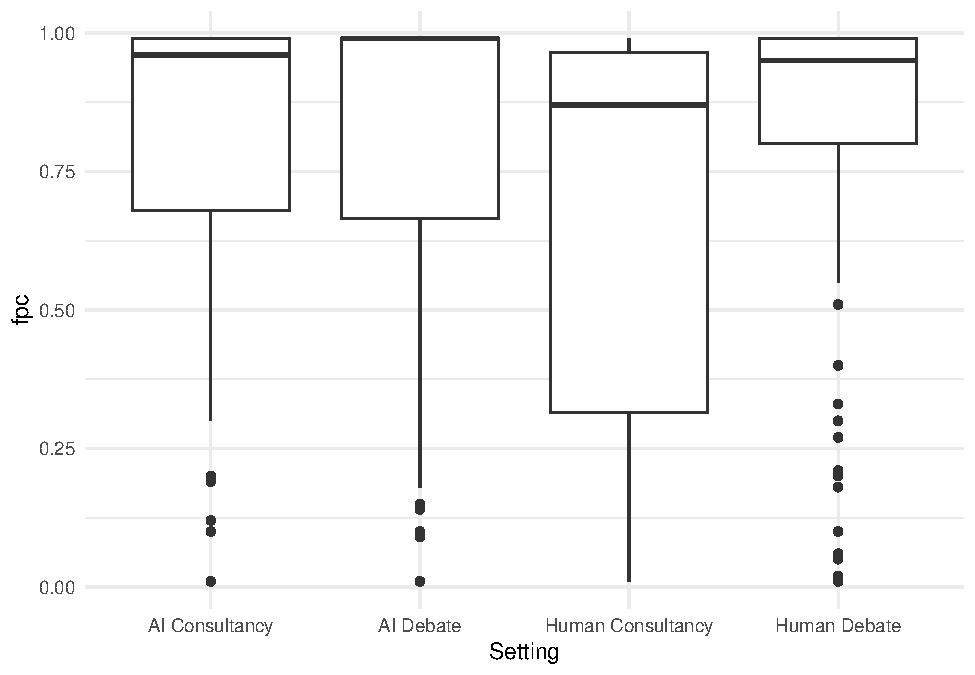
\includegraphics{debate-2309_files/figure-latex/final probability correct-1.pdf}

\begin{Shaded}
\begin{Highlighting}[]
\NormalTok{judgments\_online }\SpecialCharTok{\%\textgreater{}\%}
  \FunctionTok{group\_by}\NormalTok{(Final\_Setting) }\SpecialCharTok{\%\textgreater{}\%} \FunctionTok{summarise}\NormalTok{(}\AttributeTok{fpcmed =} \FunctionTok{median}\NormalTok{(fpc),}
                                                           \AttributeTok{fpcmean =} \FunctionTok{mean}\NormalTok{(Final\_Accuracy)) }\SpecialCharTok{\%\textgreater{}\%}
  \FunctionTok{ggplot}\NormalTok{() }\SpecialCharTok{+}
  \FunctionTok{geom\_boxplot}\NormalTok{(}\FunctionTok{aes}\NormalTok{(}\AttributeTok{x =}\NormalTok{ Final\_Setting, }\AttributeTok{y =}\NormalTok{ fpcmean)) }\SpecialCharTok{+}
  \FunctionTok{labs}\NormalTok{(}\AttributeTok{y =} \StringTok{"acc"}\NormalTok{, }\AttributeTok{x =} \StringTok{"Setting"}\NormalTok{)}\SpecialCharTok{+}
  \FunctionTok{theme\_minimal}\NormalTok{()}
\end{Highlighting}
\end{Shaded}

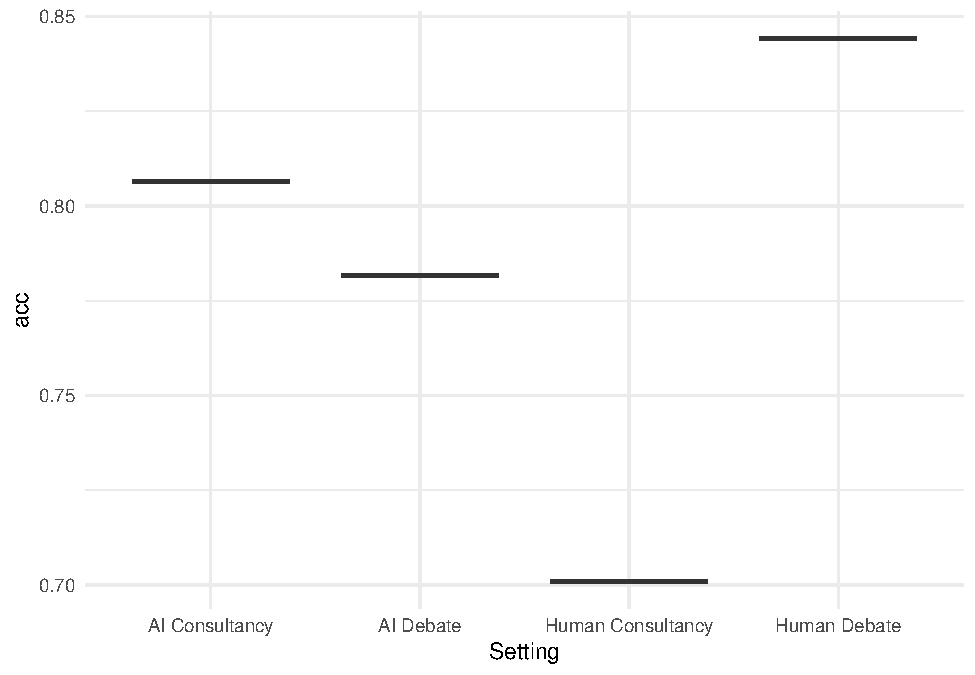
\includegraphics{debate-2309_files/figure-latex/final probability correct-2.pdf}

\begin{Shaded}
\begin{Highlighting}[]
\NormalTok{consultancy\_design }\OtherTok{\textless{}{-}} \FunctionTok{svydesign}\NormalTok{(}\AttributeTok{ids =} \SpecialCharTok{\textasciitilde{}}\DecValTok{1}\NormalTok{, }\AttributeTok{data =} \FunctionTok{subset}\NormalTok{(judgments\_online, }\StringTok{\textasciigrave{}}\AttributeTok{Consultancy Sample}\StringTok{\textasciigrave{}} \SpecialCharTok{==} \ConstantTok{TRUE} \SpecialCharTok{|} \SpecialCharTok{!}\FunctionTok{grepl}\NormalTok{(}\StringTok{"Consultancy"}\NormalTok{, Final\_Setting)), }\AttributeTok{weights =} \SpecialCharTok{\textasciitilde{}}\NormalTok{sampled\_consultancies\_all\_debates\_weights\_grouped\_setting)}



\NormalTok{human\_consultancy\_design }\OtherTok{\textless{}{-}} \FunctionTok{svydesign}\NormalTok{(}\AttributeTok{ids =} \SpecialCharTok{\textasciitilde{}}\DecValTok{1}\NormalTok{, }\AttributeTok{data =} \FunctionTok{subset}\NormalTok{(judgments\_online, }\StringTok{\textasciigrave{}}\AttributeTok{Human Consultancy Sample}\StringTok{\textasciigrave{}} \SpecialCharTok{==} \ConstantTok{TRUE} \SpecialCharTok{|} \SpecialCharTok{!}\FunctionTok{grepl}\NormalTok{(}\StringTok{"Consultancy"}\NormalTok{, Final\_Setting) }\SpecialCharTok{\&} \SpecialCharTok{!}\FunctionTok{grepl}\NormalTok{(}\StringTok{"AI"}\NormalTok{, Final\_Setting)), }\AttributeTok{weights =} \SpecialCharTok{\textasciitilde{}}\NormalTok{sampled\_consultancies\_all\_debates\_weights\_grouped\_setting)}


\FunctionTok{svyranktest}\NormalTok{(fpc}\SpecialCharTok{\textasciitilde{}}\NormalTok{Final\_Setting, human\_consultancy\_design)}
\end{Highlighting}
\end{Shaded}

\begin{verbatim}
## 
##  Design-based KruskalWallis test
## 
## data:  fpc ~ Final_Setting
## t = 2.4508, df = 235, p-value = 0.01499
## alternative hypothesis: true difference in mean rank score is not equal to 0
## sample estimates:
## difference in mean rank score 
##                     0.0969166
\end{verbatim}

\begin{Shaded}
\begin{Highlighting}[]
\NormalTok{judgments\_online }\SpecialCharTok{\%\textgreater{}\%} \FunctionTok{group\_by}\NormalTok{(Final\_Setting) }\SpecialCharTok{\%\textgreater{}\%} \FunctionTok{summarise}\NormalTok{(}\AttributeTok{fpcmed =} \FunctionTok{median}\NormalTok{(fpc),}
                                                           \AttributeTok{fpcmean =} \FunctionTok{mean}\NormalTok{(fpc))}
\end{Highlighting}
\end{Shaded}

\begin{verbatim}
## # A tibble: 4 x 3
##   Final_Setting     fpcmed fpcmean
##   <chr>              <dbl>   <dbl>
## 1 AI Consultancy      0.96   0.764
## 2 AI Debate           0.99   0.754
## 3 Human Consultancy   0.87   0.672
## 4 Human Debate        0.95   0.792
\end{verbatim}

\begin{Shaded}
\begin{Highlighting}[]
\FunctionTok{svyranktest}\NormalTok{(fpc}\SpecialCharTok{\textasciitilde{}}\NormalTok{Final\_Setting, consultancy\_design, }\AttributeTok{test =} \StringTok{"median"}\NormalTok{)}
\end{Highlighting}
\end{Shaded}

\begin{verbatim}
## 
##  Design-based median test
## 
## data:  fpc ~ Final_Setting
## df = 3, Chisq = 13.969, p-value = 0.003272
\end{verbatim}

\begin{Shaded}
\begin{Highlighting}[]
\FunctionTok{svyranktest}\NormalTok{(fpc}\SpecialCharTok{\textasciitilde{}}\NormalTok{Final\_Setting, consultancy\_design, }\AttributeTok{test =} \StringTok{"wilcoxon"}\NormalTok{)}
\end{Highlighting}
\end{Shaded}

\begin{verbatim}
## 
##  Design-based KruskalWallis test
## 
## data:  fpc ~ Final_Setting
## df = 3, Chisq = 12.446, p-value = 0.006514
\end{verbatim}

\begin{Shaded}
\begin{Highlighting}[]
\FunctionTok{svyranktest}\NormalTok{(fpc}\SpecialCharTok{\textasciitilde{}}\NormalTok{Final\_Setting, consultancy\_design, }\AttributeTok{test =} \StringTok{"vanderWaerden"}\NormalTok{)}
\end{Highlighting}
\end{Shaded}

\begin{verbatim}
## 
##  Design-based vanderWaerden test
## 
## data:  fpc ~ Final_Setting
## df = 3, Chisq = 9.8037, p-value = 0.02133
\end{verbatim}

\begin{Shaded}
\begin{Highlighting}[]
\FunctionTok{weighted\_mannwhitney}\NormalTok{(fpc }\SpecialCharTok{\textasciitilde{}}\NormalTok{ Final\_Setting }\SpecialCharTok{+}\NormalTok{ sampled\_consultancies\_all\_debates\_weights\_grouped\_setting, judgments\_online)}
\end{Highlighting}
\end{Shaded}

\begin{verbatim}
## Warning in summary.glm(glm.object): observations with zero weight not used for
## calculating dispersion
\end{verbatim}

\begin{verbatim}
## 
## # Weighted Kruskal-Wallis test
## 
##   comparison of fpc by Final_Setting
##   Chisq=3.00  df=12  p-value=0.006
\end{verbatim}

\begin{Shaded}
\begin{Highlighting}[]
\FunctionTok{weighted\_mannwhitney}\NormalTok{(fpc }\SpecialCharTok{\textasciitilde{}}\NormalTok{ Final\_Setting }\SpecialCharTok{+}\NormalTok{ sampled\_consultancies\_all\_debates\_weights\_grouped\_setting, judgments\_online)}
\end{Highlighting}
\end{Shaded}

\begin{verbatim}
## Warning in summary.glm(glm.object): observations with zero weight not used for
## calculating dispersion
\end{verbatim}

\begin{verbatim}
## 
## # Weighted Kruskal-Wallis test
## 
##   comparison of fpc by Final_Setting
##   Chisq=3.00  df=12  p-value=0.006
\end{verbatim}

\subsubsection{Logistic regression}\label{logistic-regression}

\begin{Shaded}
\begin{Highlighting}[]
\CommentTok{\#judgments\_online$Final\_Setting \textless{}{-} relevel(judgments\_online$Final\_Setting, ref = "Human Debate")}
\NormalTok{model1 }\OtherTok{\textless{}{-}} \FunctionTok{glm}\NormalTok{(Final\_Accuracy }\SpecialCharTok{\textasciitilde{}} \FunctionTok{relevel}\NormalTok{(}\FunctionTok{factor}\NormalTok{(Final\_Setting), }\StringTok{\textquotesingle{}Human Debate\textquotesingle{}}\NormalTok{), }\AttributeTok{family =} \StringTok{\textquotesingle{}binomial\textquotesingle{}}\NormalTok{, }\AttributeTok{data =}\NormalTok{ judgments\_online)}

\FunctionTok{summary}\NormalTok{(model1)}
\end{Highlighting}
\end{Shaded}

\begin{verbatim}
## 
## Call:
## glm(formula = Final_Accuracy ~ relevel(factor(Final_Setting), 
##     "Human Debate"), family = "binomial", data = judgments_online)
## 
## Coefficients:
##                                                                 Estimate
## (Intercept)                                                       1.6487
## relevel(factor(Final_Setting), "Human Debate")AI Consultancy     -0.2215
## relevel(factor(Final_Setting), "Human Debate")AI Debate          -0.3736
## relevel(factor(Final_Setting), "Human Debate")Human Consultancy  -0.7969
##                                                                 Std. Error
## (Intercept)                                                         0.2184
## relevel(factor(Final_Setting), "Human Debate")AI Consultancy        0.3414
## relevel(factor(Final_Setting), "Human Debate")AI Debate             0.3392
## relevel(factor(Final_Setting), "Human Debate")Human Consultancy     0.3038
##                                                                 z value
## (Intercept)                                                       7.549
## relevel(factor(Final_Setting), "Human Debate")AI Consultancy     -0.649
## relevel(factor(Final_Setting), "Human Debate")AI Debate          -1.102
## relevel(factor(Final_Setting), "Human Debate")Human Consultancy  -2.623
##                                                                           Pr(>|z|)
## (Intercept)                                                     0.0000000000000438
## relevel(factor(Final_Setting), "Human Debate")AI Consultancy               0.51644
## relevel(factor(Final_Setting), "Human Debate")AI Debate                    0.27067
## relevel(factor(Final_Setting), "Human Debate")Human Consultancy            0.00871
##                                                                    
## (Intercept)                                                     ***
## relevel(factor(Final_Setting), "Human Debate")AI Consultancy       
## relevel(factor(Final_Setting), "Human Debate")AI Debate            
## relevel(factor(Final_Setting), "Human Debate")Human Consultancy ** 
## ---
## Signif. codes:  0 '***' 0.001 '**' 0.01 '*' 0.05 '.' 0.1 ' ' 1
## 
## (Dispersion parameter for binomial family taken to be 1)
## 
##     Null deviance: 457.45  on 441  degrees of freedom
## Residual deviance: 450.23  on 438  degrees of freedom
## AIC: 458.23
## 
## Number of Fisher Scoring iterations: 4
\end{verbatim}

\begin{Shaded}
\begin{Highlighting}[]
\FunctionTok{table}\NormalTok{(model1}\SpecialCharTok{$}\NormalTok{fitted.values }\SpecialCharTok{\textgreater{}} \FloatTok{0.5}\NormalTok{) }
\end{Highlighting}
\end{Shaded}

\begin{verbatim}
## 
## TRUE 
##  442
\end{verbatim}

\begin{Shaded}
\begin{Highlighting}[]
\FunctionTok{table}\NormalTok{(judgments\_online}\SpecialCharTok{$}\NormalTok{Final\_Accuracy)}
\end{Highlighting}
\end{Shaded}

\begin{verbatim}
## 
## FALSE  TRUE 
##    94   348
\end{verbatim}

\begin{Shaded}
\begin{Highlighting}[]
\NormalTok{model2 }\OtherTok{\textless{}{-}} \FunctionTok{glm}\NormalTok{(Final\_Accuracy }\SpecialCharTok{\textasciitilde{}} \FunctionTok{relevel}\NormalTok{(}\FunctionTok{factor}\NormalTok{(Participant),}\StringTok{\textquotesingle{}Aliyaah Toussaint\textquotesingle{}}\NormalTok{) }\SpecialCharTok{+} \FunctionTok{relevel}\NormalTok{(}\FunctionTok{factor}\NormalTok{(Final\_Setting), }\StringTok{\textquotesingle{}Human Debate\textquotesingle{}}\NormalTok{), }\AttributeTok{family =} \StringTok{\textquotesingle{}binomial\textquotesingle{}}\NormalTok{, }\AttributeTok{data =}\NormalTok{ judgments\_online)}

\FunctionTok{summary}\NormalTok{(model2)}
\end{Highlighting}
\end{Shaded}

\begin{verbatim}
## 
## Call:
## glm(formula = Final_Accuracy ~ relevel(factor(Participant), "Aliyaah Toussaint") + 
##     relevel(factor(Final_Setting), "Human Debate"), family = "binomial", 
##     data = judgments_online)
## 
## Coefficients:
##                                                                       Estimate
## (Intercept)                                                            2.19432
## relevel(factor(Participant), "Aliyaah Toussaint")Adelle Fernando      -0.79600
## relevel(factor(Participant), "Aliyaah Toussaint")Anuj Jain            -0.89691
## relevel(factor(Participant), "Aliyaah Toussaint")David Rein           -0.43887
## relevel(factor(Participant), "Aliyaah Toussaint")Emmanuel Makinde    -17.76039
## relevel(factor(Participant), "Aliyaah Toussaint")Ethan Rosen          -0.24841
## relevel(factor(Participant), "Aliyaah Toussaint")Jackson Petty        -0.55820
## relevel(factor(Participant), "Aliyaah Toussaint")Jessica Li           -0.16347
## relevel(factor(Participant), "Aliyaah Toussaint")Julian Michael       -0.08063
## relevel(factor(Participant), "Aliyaah Toussaint")Julien Dirani        13.37175
## relevel(factor(Participant), "Aliyaah Toussaint")Max Layden           13.37175
## relevel(factor(Participant), "Aliyaah Toussaint")Noor Mirza-Rashid    -1.27803
## relevel(factor(Participant), "Aliyaah Toussaint")Reeya Kansra         -0.96379
## relevel(factor(Participant), "Aliyaah Toussaint")Salsabila Mahdi      -0.17942
## relevel(factor(Participant), "Aliyaah Toussaint")Sam Jin              -0.01031
## relevel(factor(Participant), "Aliyaah Toussaint")Sean Wang             0.17177
## relevel(factor(Participant), "Aliyaah Toussaint")Shlomo Kofman        -1.13135
## relevel(factor(Participant), "Aliyaah Toussaint")Shreeram Modi        -1.16733
## relevel(factor(Participant), "Aliyaah Toussaint")Vishakh Padmakumar   -0.40256
## relevel(factor(Final_Setting), "Human Debate")AI Consultancy          -0.27193
## relevel(factor(Final_Setting), "Human Debate")AI Debate               -0.42241
## relevel(factor(Final_Setting), "Human Debate")Human Consultancy       -0.74485
##                                                                     Std. Error
## (Intercept)                                                            0.49853
## relevel(factor(Participant), "Aliyaah Toussaint")Adelle Fernando       0.63661
## relevel(factor(Participant), "Aliyaah Toussaint")Anuj Jain             0.53893
## relevel(factor(Participant), "Aliyaah Toussaint")David Rein            0.77471
## relevel(factor(Participant), "Aliyaah Toussaint")Emmanuel Makinde   1455.39762
## relevel(factor(Participant), "Aliyaah Toussaint")Ethan Rosen           1.17957
## relevel(factor(Participant), "Aliyaah Toussaint")Jackson Petty         0.66085
## relevel(factor(Participant), "Aliyaah Toussaint")Jessica Li            0.64365
## relevel(factor(Participant), "Aliyaah Toussaint")Julian Michael        0.75783
## relevel(factor(Participant), "Aliyaah Toussaint")Julien Dirani      1029.12159
## relevel(factor(Participant), "Aliyaah Toussaint")Max Layden         1029.12159
## relevel(factor(Participant), "Aliyaah Toussaint")Noor Mirza-Rashid     0.97393
## relevel(factor(Participant), "Aliyaah Toussaint")Reeya Kansra          0.58143
## relevel(factor(Participant), "Aliyaah Toussaint")Salsabila Mahdi       0.90289
## relevel(factor(Participant), "Aliyaah Toussaint")Sam Jin               0.56587
## relevel(factor(Participant), "Aliyaah Toussaint")Sean Wang             0.67879
## relevel(factor(Participant), "Aliyaah Toussaint")Shlomo Kofman         0.50759
## relevel(factor(Participant), "Aliyaah Toussaint")Shreeram Modi         0.63420
## relevel(factor(Participant), "Aliyaah Toussaint")Vishakh Padmakumar    1.18962
## relevel(factor(Final_Setting), "Human Debate")AI Consultancy           0.39222
## relevel(factor(Final_Setting), "Human Debate")AI Debate                0.39204
## relevel(factor(Final_Setting), "Human Debate")Human Consultancy        0.36432
##                                                                     z value
## (Intercept)                                                           4.402
## relevel(factor(Participant), "Aliyaah Toussaint")Adelle Fernando     -1.250
## relevel(factor(Participant), "Aliyaah Toussaint")Anuj Jain           -1.664
## relevel(factor(Participant), "Aliyaah Toussaint")David Rein          -0.566
## relevel(factor(Participant), "Aliyaah Toussaint")Emmanuel Makinde    -0.012
## relevel(factor(Participant), "Aliyaah Toussaint")Ethan Rosen         -0.211
## relevel(factor(Participant), "Aliyaah Toussaint")Jackson Petty       -0.845
## relevel(factor(Participant), "Aliyaah Toussaint")Jessica Li          -0.254
## relevel(factor(Participant), "Aliyaah Toussaint")Julian Michael      -0.106
## relevel(factor(Participant), "Aliyaah Toussaint")Julien Dirani        0.013
## relevel(factor(Participant), "Aliyaah Toussaint")Max Layden           0.013
## relevel(factor(Participant), "Aliyaah Toussaint")Noor Mirza-Rashid   -1.312
## relevel(factor(Participant), "Aliyaah Toussaint")Reeya Kansra        -1.658
## relevel(factor(Participant), "Aliyaah Toussaint")Salsabila Mahdi     -0.199
## relevel(factor(Participant), "Aliyaah Toussaint")Sam Jin             -0.018
## relevel(factor(Participant), "Aliyaah Toussaint")Sean Wang            0.253
## relevel(factor(Participant), "Aliyaah Toussaint")Shlomo Kofman       -2.229
## relevel(factor(Participant), "Aliyaah Toussaint")Shreeram Modi       -1.841
## relevel(factor(Participant), "Aliyaah Toussaint")Vishakh Padmakumar  -0.338
## relevel(factor(Final_Setting), "Human Debate")AI Consultancy         -0.693
## relevel(factor(Final_Setting), "Human Debate")AI Debate              -1.077
## relevel(factor(Final_Setting), "Human Debate")Human Consultancy      -2.045
##                                                                      Pr(>|z|)
## (Intercept)                                                         0.0000107
## relevel(factor(Participant), "Aliyaah Toussaint")Adelle Fernando       0.2112
## relevel(factor(Participant), "Aliyaah Toussaint")Anuj Jain             0.0961
## relevel(factor(Participant), "Aliyaah Toussaint")David Rein            0.5711
## relevel(factor(Participant), "Aliyaah Toussaint")Emmanuel Makinde      0.9903
## relevel(factor(Participant), "Aliyaah Toussaint")Ethan Rosen           0.8332
## relevel(factor(Participant), "Aliyaah Toussaint")Jackson Petty         0.3983
## relevel(factor(Participant), "Aliyaah Toussaint")Jessica Li            0.7995
## relevel(factor(Participant), "Aliyaah Toussaint")Julian Michael        0.9153
## relevel(factor(Participant), "Aliyaah Toussaint")Julien Dirani         0.9896
## relevel(factor(Participant), "Aliyaah Toussaint")Max Layden            0.9896
## relevel(factor(Participant), "Aliyaah Toussaint")Noor Mirza-Rashid     0.1894
## relevel(factor(Participant), "Aliyaah Toussaint")Reeya Kansra          0.0974
## relevel(factor(Participant), "Aliyaah Toussaint")Salsabila Mahdi       0.8425
## relevel(factor(Participant), "Aliyaah Toussaint")Sam Jin               0.9855
## relevel(factor(Participant), "Aliyaah Toussaint")Sean Wang             0.8002
## relevel(factor(Participant), "Aliyaah Toussaint")Shlomo Kofman         0.0258
## relevel(factor(Participant), "Aliyaah Toussaint")Shreeram Modi         0.0657
## relevel(factor(Participant), "Aliyaah Toussaint")Vishakh Padmakumar    0.7351
## relevel(factor(Final_Setting), "Human Debate")AI Consultancy           0.4881
## relevel(factor(Final_Setting), "Human Debate")AI Debate                0.2813
## relevel(factor(Final_Setting), "Human Debate")Human Consultancy        0.0409
##                                                                        
## (Intercept)                                                         ***
## relevel(factor(Participant), "Aliyaah Toussaint")Adelle Fernando       
## relevel(factor(Participant), "Aliyaah Toussaint")Anuj Jain          .  
## relevel(factor(Participant), "Aliyaah Toussaint")David Rein            
## relevel(factor(Participant), "Aliyaah Toussaint")Emmanuel Makinde      
## relevel(factor(Participant), "Aliyaah Toussaint")Ethan Rosen           
## relevel(factor(Participant), "Aliyaah Toussaint")Jackson Petty         
## relevel(factor(Participant), "Aliyaah Toussaint")Jessica Li            
## relevel(factor(Participant), "Aliyaah Toussaint")Julian Michael        
## relevel(factor(Participant), "Aliyaah Toussaint")Julien Dirani         
## relevel(factor(Participant), "Aliyaah Toussaint")Max Layden            
## relevel(factor(Participant), "Aliyaah Toussaint")Noor Mirza-Rashid     
## relevel(factor(Participant), "Aliyaah Toussaint")Reeya Kansra       .  
## relevel(factor(Participant), "Aliyaah Toussaint")Salsabila Mahdi       
## relevel(factor(Participant), "Aliyaah Toussaint")Sam Jin               
## relevel(factor(Participant), "Aliyaah Toussaint")Sean Wang             
## relevel(factor(Participant), "Aliyaah Toussaint")Shlomo Kofman      *  
## relevel(factor(Participant), "Aliyaah Toussaint")Shreeram Modi      .  
## relevel(factor(Participant), "Aliyaah Toussaint")Vishakh Padmakumar    
## relevel(factor(Final_Setting), "Human Debate")AI Consultancy           
## relevel(factor(Final_Setting), "Human Debate")AI Debate                
## relevel(factor(Final_Setting), "Human Debate")Human Consultancy     *  
## ---
## Signif. codes:  0 '***' 0.001 '**' 0.01 '*' 0.05 '.' 0.1 ' ' 1
## 
## (Dispersion parameter for binomial family taken to be 1)
## 
##     Null deviance: 457.45  on 441  degrees of freedom
## Residual deviance: 429.05  on 420  degrees of freedom
## AIC: 473.05
## 
## Number of Fisher Scoring iterations: 14
\end{verbatim}

\subsubsection{LMER}\label{lmer}

\begin{Shaded}
\begin{Highlighting}[]
\NormalTok{random.intercept.model }\OtherTok{=} \FunctionTok{lmer}\NormalTok{(}\StringTok{\textasciigrave{}}\AttributeTok{Final probability correct}\StringTok{\textasciigrave{}} \SpecialCharTok{\textasciitilde{}}\NormalTok{ (}\DecValTok{1}\SpecialCharTok{|}\NormalTok{Final\_Setting), }
                              \AttributeTok{data =}\NormalTok{ judgments, }\AttributeTok{REML =} \ConstantTok{TRUE}\NormalTok{)}
\NormalTok{judgments}\SpecialCharTok{$}\NormalTok{random.intercept.preds }\OtherTok{=} \FunctionTok{predict}\NormalTok{(random.intercept.model)}
\FunctionTok{summary}\NormalTok{(random.intercept.model)}
\end{Highlighting}
\end{Shaded}

\begin{verbatim}
## Linear mixed model fit by REML. t-tests use Satterthwaite's method [
## lmerModLmerTest]
## Formula: `Final probability correct` ~ (1 | Final_Setting)
##    Data: judgments
## 
## REML criterion at convergence: 364
## 
## Scaled residuals: 
##     Min      1Q  Median      3Q     Max 
## -2.5652 -0.2013  0.5015  0.5654  0.9255 
## 
## Random effects:
##  Groups        Name        Variance Std.Dev.
##  Final_Setting (Intercept) 0.00272  0.05215 
##  Residual                  0.09799  0.31304 
## Number of obs: 686, groups:  Final_Setting, 4
## 
## Fixed effects:
##             Estimate Std. Error      df t value Pr(>|t|)    
## (Intercept)  0.75723    0.02948 3.33321   25.68  0.00006 ***
## ---
## Signif. codes:  0 '***' 0.001 '**' 0.01 '*' 0.05 '.' 0.1 ' ' 1
\end{verbatim}

\begin{Shaded}
\begin{Highlighting}[]
\FunctionTok{ranef}\NormalTok{(random.intercept.model)}
\end{Highlighting}
\end{Shaded}

\begin{verbatim}
## $Final_Setting
##                    (Intercept)
## AI Consultancy     0.002319435
## AI Debate         -0.001131440
## Human Consultancy -0.056960042
## Human Debate       0.055772047
## 
## with conditional variances for "Final_Setting"
\end{verbatim}

\begin{Shaded}
\begin{Highlighting}[]
\FunctionTok{ranova}\NormalTok{(random.intercept.model)}
\end{Highlighting}
\end{Shaded}

\begin{verbatim}
## ANOVA-like table for random-effects: Single term deletions
## 
## Model:
## `Final probability correct` ~ (1 | Final_Setting)
##                     npar  logLik    AIC    LRT Df Pr(>Chisq)   
## <none>                 3 -182.00 370.00                        
## (1 | Final_Setting)    2 -187.23 378.46 10.456  1   0.001222 **
## ---
## Signif. codes:  0 '***' 0.001 '**' 0.01 '*' 0.05 '.' 0.1 ' ' 1
\end{verbatim}

\begin{Shaded}
\begin{Highlighting}[]
\NormalTok{random.intercept.model }\OtherTok{=} \FunctionTok{lmer}\NormalTok{(}\StringTok{\textasciigrave{}}\AttributeTok{Final probability correct}\StringTok{\textasciigrave{}} \SpecialCharTok{\textasciitilde{}}\NormalTok{ (}\DecValTok{1}\SpecialCharTok{|}\NormalTok{Participant) }\SpecialCharTok{+}\NormalTok{ (}\DecValTok{1}\SpecialCharTok{|}\NormalTok{Final\_Setting), }
                              \AttributeTok{data =}\NormalTok{ judgments, }\AttributeTok{REML =} \ConstantTok{TRUE}\NormalTok{)}
\NormalTok{judgments}\SpecialCharTok{$}\NormalTok{random.intercept.preds }\OtherTok{=} \FunctionTok{predict}\NormalTok{(random.intercept.model)}
\FunctionTok{summary}\NormalTok{(random.intercept.model)}
\end{Highlighting}
\end{Shaded}

\begin{verbatim}
## Linear mixed model fit by REML. t-tests use Satterthwaite's method [
## lmerModLmerTest]
## Formula: `Final probability correct` ~ (1 | Participant) + (1 | Final_Setting)
##    Data: judgments
## 
## REML criterion at convergence: 357.9
## 
## Scaled residuals: 
##     Min      1Q  Median      3Q     Max 
## -2.7461 -0.1555  0.4368  0.5996  1.1083 
## 
## Random effects:
##  Groups        Name        Variance Std.Dev.
##  Participant   (Intercept) 0.002215 0.04707 
##  Final_Setting (Intercept) 0.002718 0.05213 
##  Residual                  0.095721 0.30939 
## Number of obs: 686, groups:  Participant, 19; Final_Setting, 4
## 
## Fixed effects:
##             Estimate Std. Error      df t value   Pr(>|t|)    
## (Intercept)  0.75549    0.03211 4.44845   23.52 0.00000772 ***
## ---
## Signif. codes:  0 '***' 0.001 '**' 0.01 '*' 0.05 '.' 0.1 ' ' 1
\end{verbatim}

\begin{Shaded}
\begin{Highlighting}[]
\FunctionTok{ranef}\NormalTok{(random.intercept.model)}
\end{Highlighting}
\end{Shaded}

\begin{verbatim}
## $Participant
##                      (Intercept)
## Adelle Fernando    -0.0231887667
## Aliyaah Toussaint   0.0445495902
## Anuj Jain          -0.0460548530
## David Rein          0.0107246587
## Emmanuel Makinde   -0.0115704647
## Ethan Rosen        -0.0171199427
## Jackson Petty      -0.0051104119
## Jessica Li         -0.0047621455
## Julian Michael      0.0348708056
## Julien Dirani      -0.0008138972
## Max Layden         -0.0038287458
## Noor Mirza-Rashid  -0.0117445230
## Reeya Kansra       -0.0261229696
## Salsabila Mahdi     0.0321800144
## Sam Jin             0.0480694982
## Sean Wang           0.0477306783
## Shlomo Kofman      -0.0519667486
## Shreeram Modi       0.0020512016
## Vishakh Padmakumar -0.0178929784
## 
## $Final_Setting
##                     (Intercept)
## AI Consultancy     0.0012586597
## AI Debate         -0.0009034629
## Human Consultancy -0.0564188188
## Human Debate       0.0560636219
## 
## with conditional variances for "Participant" "Final_Setting"
\end{verbatim}

\begin{Shaded}
\begin{Highlighting}[]
\FunctionTok{ranova}\NormalTok{(random.intercept.model)}
\end{Highlighting}
\end{Shaded}

\begin{verbatim}
## ANOVA-like table for random-effects: Single term deletions
## 
## Model:
## `Final probability correct` ~ (1 | Participant) + (1 | Final_Setting)
##                     npar  logLik   AIC    LRT Df Pr(>Chisq)   
## <none>                 4 -178.95 365.9                        
## (1 | Participant)      3 -182.00 370.0 6.0957  1   0.013551 * 
## (1 | Final_Setting)    3 -183.65 373.3 9.4004  1   0.002169 **
## ---
## Signif. codes:  0 '***' 0.001 '**' 0.01 '*' 0.05 '.' 0.1 ' ' 1
\end{verbatim}

\subsubsection{BRMS}\label{brms}

\begin{Shaded}
\begin{Highlighting}[]
\CommentTok{\#brm1 \textless{}{-} brm(data = judgments\_online,}
\CommentTok{\#             formula = as.numeric(Final\_Accuracy) | trials(2) \textasciitilde{} 1 + (1 | Final\_Setting),}
\CommentTok{\#             family = binomial("identity"),}
\CommentTok{\#             iter = 2000, warmup = 1000, chains = 4, cores = 4,}
\CommentTok{\#             control = list(adapt\_delta = .975, max\_treedepth = 20),}
\CommentTok{\#             seed = 190831)}
\CommentTok{\#plot(brm1)}
\end{Highlighting}
\end{Shaded}

\subsection{Efficiency}\label{efficiency}

\subsubsection{Quotes \%, caveats}\label{quotes-caveats}

\begin{Shaded}
\begin{Highlighting}[]
\NormalTok{characters }\OperatorTok{=}\NormalTok{ turns.merge(}
\NormalTok{        debates[[}\StringTok{"Room name"}\NormalTok{, }\StringTok{"Question"}\NormalTok{, }\StringTok{"Story length"}\NormalTok{,}
                 \StringTok{"Untimed annotator context"}\NormalTok{,}\StringTok{"Untimed annotator context bins"}\NormalTok{,}
                 \StringTok{"Setting"}\NormalTok{, }\StringTok{"Final\_Setting"}\NormalTok{, }\StringTok{"Final\_Accuracy"}\NormalTok{,}
                 \StringTok{"Is offline"}\NormalTok{]],}
\NormalTok{        how}\OperatorTok{=}\StringTok{"left"}\NormalTok{,}
\NormalTok{        on}\OperatorTok{=}\StringTok{"Room name"}\NormalTok{,}
\NormalTok{    )}



\CommentTok{\# Filtering for specific roles}
\NormalTok{characters }\OperatorTok{=}\NormalTok{ characters[characters[}\StringTok{\textquotesingle{}Role (honest/dishonest)\textquotesingle{}}\NormalTok{].isin([}\StringTok{\textquotesingle{}Honest debater\textquotesingle{}}\NormalTok{, }\StringTok{\textquotesingle{}Dishonest debater\textquotesingle{}}\NormalTok{])]}

\CommentTok{\# Extracting the spans}
\KeywordTok{def}\NormalTok{ extract\_spans(span\_str):}
    \CommentTok{"""Extract numerical spans from the given string."""}
    \ControlFlowTok{if}\NormalTok{ pd.isna(span\_str):}
        \ControlFlowTok{return}\NormalTok{ []}
\NormalTok{    spans }\OperatorTok{=}\NormalTok{ re.findall(}\VerbatimStringTok{r\textquotesingle{}\textless{}\textless{}(\textbackslash{}d+){-}(\textbackslash{}d+)\textgreater{}\textgreater{}\textquotesingle{}}\NormalTok{, span\_str)}
    \ControlFlowTok{return}\NormalTok{ [(}\BuiltInTok{int}\NormalTok{(start), }\BuiltInTok{int}\NormalTok{(end)) }\ControlFlowTok{for}\NormalTok{ start, end }\KeywordTok{in}\NormalTok{ spans]}

\CommentTok{\# Merging overlapping spans}
\KeywordTok{def}\NormalTok{ merge\_overlapping\_spans(span\_str):}
    \ControlFlowTok{if} \KeywordTok{not} \BuiltInTok{isinstance}\NormalTok{(span\_str, }\BuiltInTok{str}\NormalTok{):}
        \ControlFlowTok{return}\NormalTok{ span\_str}
\NormalTok{    spans }\OperatorTok{=}\NormalTok{ extract\_spans(span\_str)}
    \ControlFlowTok{if} \KeywordTok{not}\NormalTok{ spans:}
        \ControlFlowTok{return}\NormalTok{ span\_str}
\NormalTok{    spans.sort(key}\OperatorTok{=}\KeywordTok{lambda}\NormalTok{ x: x[}\DecValTok{0}\NormalTok{])}
\NormalTok{    merged }\OperatorTok{=}\NormalTok{ [spans[}\DecValTok{0}\NormalTok{]]}
    \ControlFlowTok{for}\NormalTok{ current }\KeywordTok{in}\NormalTok{ spans:}
\NormalTok{        previous }\OperatorTok{=}\NormalTok{ merged[}\OperatorTok{{-}}\DecValTok{1}\NormalTok{]}
        \ControlFlowTok{if}\NormalTok{ current[}\DecValTok{0}\NormalTok{] }\OperatorTok{\textless{}=}\NormalTok{ previous[}\DecValTok{1}\NormalTok{]:}
\NormalTok{            upper\_bound }\OperatorTok{=} \BuiltInTok{max}\NormalTok{(previous[}\DecValTok{1}\NormalTok{], current[}\DecValTok{1}\NormalTok{])}
\NormalTok{            merged[}\OperatorTok{{-}}\DecValTok{1}\NormalTok{] }\OperatorTok{=}\NormalTok{ (previous[}\DecValTok{0}\NormalTok{], upper\_bound)}
        \ControlFlowTok{else}\NormalTok{:}
\NormalTok{            merged.append(current)}
    \ControlFlowTok{return} \StringTok{\textquotesingle{} \textquotesingle{}}\NormalTok{.join(}\SpecialStringTok{f\textquotesingle{}\textless{}\textless{}}\SpecialCharTok{\{}\NormalTok{start}\SpecialCharTok{\}}\SpecialStringTok{{-}}\SpecialCharTok{\{}\NormalTok{end}\SpecialCharTok{\}}\SpecialStringTok{\textgreater{}\textgreater{}\textquotesingle{}} \ControlFlowTok{for}\NormalTok{ start, end }\KeywordTok{in}\NormalTok{ merged)}

\CommentTok{\# Aggregating function to concatenate quote spans}
\KeywordTok{def}\NormalTok{ custom\_join(series):}
    \ControlFlowTok{return} \StringTok{\textquotesingle{} \textquotesingle{}}\NormalTok{.join(}\BuiltInTok{filter}\NormalTok{(}\KeywordTok{lambda}\NormalTok{ x: }\BuiltInTok{isinstance}\NormalTok{(x, }\BuiltInTok{str}\NormalTok{), series))}

\CommentTok{\# Identify questions with more than one setting and filter out the characters dataframe}
\NormalTok{questions\_with\_multi\_settings }\OperatorTok{=}\NormalTok{ characters.groupby(}\StringTok{"Question"}\NormalTok{).}\BuiltInTok{filter}\NormalTok{(}\KeywordTok{lambda}\NormalTok{ x: }\BuiltInTok{len}\NormalTok{(x[}\StringTok{"Setting"}\NormalTok{].unique()) }\OperatorTok{\textgreater{}} \DecValTok{1}\NormalTok{)[}\StringTok{"Question"}\NormalTok{].unique()}
\NormalTok{filtered\_characters }\OperatorTok{=}\NormalTok{ characters[characters[}\StringTok{"Question"}\NormalTok{].isin(questions\_with\_multi\_settings)]}

\CommentTok{\# Aggregating data}
\NormalTok{aggregates }\OperatorTok{=}\NormalTok{ \{}
    \StringTok{\textquotesingle{}Quote length\textquotesingle{}}\NormalTok{: }\StringTok{\textquotesingle{}sum\textquotesingle{}}\NormalTok{,}
    \StringTok{\textquotesingle{}Story length\textquotesingle{}}\NormalTok{: }\StringTok{\textquotesingle{}mean\textquotesingle{}}\NormalTok{,}
    \StringTok{\textquotesingle{}Num previous judging rounds\textquotesingle{}}\NormalTok{: }\StringTok{\textquotesingle{}max\textquotesingle{}}\NormalTok{,}
    \StringTok{\textquotesingle{}Participant quote span\textquotesingle{}}\NormalTok{: custom\_join}
\NormalTok{\}}
\CommentTok{\# Grouping by \textquotesingle{}Room name\textquotesingle{} and aggregating}
\NormalTok{characters\_agg\_by\_room }\OperatorTok{=}\NormalTok{ filtered\_characters.groupby(}\StringTok{\textquotesingle{}Room name\textquotesingle{}}\NormalTok{).agg(aggregates).reset\_index()}

\CommentTok{\# Merging the aggregated results with the original data to reintroduce the desired columns}
\NormalTok{characters\_agg }\OperatorTok{=}\NormalTok{ characters\_agg\_by\_room.merge(}
\NormalTok{    filtered\_characters[[}\StringTok{\textquotesingle{}Room name\textquotesingle{}}\NormalTok{, }\StringTok{\textquotesingle{}Setting\textquotesingle{}}\NormalTok{, }\StringTok{\textquotesingle{}Final\_Setting\textquotesingle{}}\NormalTok{, }\StringTok{\textquotesingle{}Question\textquotesingle{}}\NormalTok{, }\StringTok{\textquotesingle{}Untimed annotator context bins\textquotesingle{}}\NormalTok{,}\StringTok{\textquotesingle{}Final\_Accuracy\textquotesingle{}}\NormalTok{]].drop\_duplicates(),}
\NormalTok{    on}\OperatorTok{=}\StringTok{\textquotesingle{}Room name\textquotesingle{}}
\NormalTok{)}

\CommentTok{\# Merge overlapping spans after the aggregation}
\NormalTok{characters\_agg[}\StringTok{"merged\_quote\_spans"}\NormalTok{] }\OperatorTok{=}\NormalTok{ characters\_agg[}\StringTok{"Participant quote span"}\NormalTok{].}\BuiltInTok{apply}\NormalTok{(merge\_overlapping\_spans)}

\CommentTok{\# Functions to compute and compare spans across settings}
\KeywordTok{def}\NormalTok{ extract\_numbers\_from\_span(span\_str):}
\NormalTok{    spans }\OperatorTok{=}\NormalTok{ extract\_spans(span\_str)}
\NormalTok{    numbers }\OperatorTok{=} \BuiltInTok{set}\NormalTok{()}
    \ControlFlowTok{for}\NormalTok{ start, end }\KeywordTok{in}\NormalTok{ spans:}
\NormalTok{        numbers.update(}\BuiltInTok{range}\NormalTok{(}\BuiltInTok{int}\NormalTok{(start), }\BuiltInTok{int}\NormalTok{(end)}\OperatorTok{+}\DecValTok{1}\NormalTok{))}
    \ControlFlowTok{return}\NormalTok{ numbers}

\KeywordTok{def}\NormalTok{ quote\_length(span\_str):}
\NormalTok{  spans }\OperatorTok{=}\NormalTok{ extract\_spans(span\_str)}
\NormalTok{  numbers }\OperatorTok{=} \BuiltInTok{set}\NormalTok{()}
  \ControlFlowTok{for}\NormalTok{ start, end }\KeywordTok{in}\NormalTok{ spans:}
\NormalTok{    numbers.update(}\BuiltInTok{range}\NormalTok{(}\BuiltInTok{int}\NormalTok{(start), }\BuiltInTok{int}\NormalTok{(end)))}
  \ControlFlowTok{return}\NormalTok{ numbers}

\NormalTok{characters\_agg[}\StringTok{"quote\_length"}\NormalTok{] }\OperatorTok{=}\NormalTok{ characters\_agg[}\StringTok{"Participant quote span"}\NormalTok{].}\BuiltInTok{apply}\NormalTok{(}\KeywordTok{lambda}\NormalTok{ row: }\BuiltInTok{len}\NormalTok{(quote\_length(row)))}
\CommentTok{\#characters\_agg["merged\_quote\_length"] = characters\_agg["Participant quote span"].apply(lambda row: len(quote\_length(row)))}
\CommentTok{\#print(characters\_agg["merged\_quote\_length"][1])}
\CommentTok{\#print((characters\_agg["merged\_quote\_length"]==characters\_agg["quote\_length"]).value\_counts())}

\CommentTok{\#print((characters\_agg[\textquotesingle{}quote\_length\textquotesingle{}].fillna(0)/characters\_agg[\textquotesingle{}Story length\textquotesingle{}].fillna(0)).describe())}


\KeywordTok{def}\NormalTok{ convert\_to\_span\_format(numbers):}
\NormalTok{    sorted\_numbers }\OperatorTok{=} \BuiltInTok{sorted}\NormalTok{(}\BuiltInTok{list}\NormalTok{(numbers))}
\NormalTok{    spans }\OperatorTok{=}\NormalTok{ []}
    \ControlFlowTok{if}\NormalTok{ sorted\_numbers:}
\NormalTok{        start }\OperatorTok{=}\NormalTok{ sorted\_numbers[}\DecValTok{0}\NormalTok{]}
\NormalTok{        end }\OperatorTok{=}\NormalTok{ sorted\_numbers[}\DecValTok{0}\NormalTok{]}
        \ControlFlowTok{for}\NormalTok{ num }\KeywordTok{in}\NormalTok{ sorted\_numbers[}\DecValTok{1}\NormalTok{:]:}
            \ControlFlowTok{if}\NormalTok{ num }\OperatorTok{==}\NormalTok{ end }\OperatorTok{+} \DecValTok{1}\NormalTok{:}
\NormalTok{                end }\OperatorTok{=}\NormalTok{ num}
            \ControlFlowTok{else}\NormalTok{:}
\NormalTok{                spans.append((start, end))}
\NormalTok{                start }\OperatorTok{=}\NormalTok{ end }\OperatorTok{=}\NormalTok{ num}
\NormalTok{        spans.append((start, end))}
    \ControlFlowTok{return} \StringTok{\textquotesingle{} \textquotesingle{}}\NormalTok{.join(}\SpecialStringTok{f\textquotesingle{}\textless{}\textless{}}\SpecialCharTok{\{}\NormalTok{start}\SpecialCharTok{\}}\SpecialStringTok{{-}}\SpecialCharTok{\{}\NormalTok{end}\SpecialCharTok{\}}\SpecialStringTok{\textgreater{}\textgreater{}\textquotesingle{}} \ControlFlowTok{for}\NormalTok{ start, end }\KeywordTok{in}\NormalTok{ spans)}

\KeywordTok{def}\NormalTok{ compute\_span\_differences(dataframe):}
\NormalTok{    differences }\OperatorTok{=}\NormalTok{ \{\}}
    \ControlFlowTok{for}\NormalTok{ question, group }\KeywordTok{in}\NormalTok{ dataframe.groupby(}\StringTok{"Question"}\NormalTok{):}
\NormalTok{        settings }\OperatorTok{=}\NormalTok{ group[}\StringTok{"Setting"}\NormalTok{].unique()}
        \ControlFlowTok{if} \BuiltInTok{len}\NormalTok{(settings) }\OperatorTok{\textgreater{}} \DecValTok{1}\NormalTok{:}
            \ControlFlowTok{for}\NormalTok{ i }\KeywordTok{in} \BuiltInTok{range}\NormalTok{(}\BuiltInTok{len}\NormalTok{(settings)):}
                \ControlFlowTok{for}\NormalTok{ j }\KeywordTok{in} \BuiltInTok{range}\NormalTok{(i}\OperatorTok{+}\DecValTok{1}\NormalTok{, }\BuiltInTok{len}\NormalTok{(settings)):}
\NormalTok{                    setting\_1 }\OperatorTok{=}\NormalTok{ settings[i]}
\NormalTok{                    setting\_2 }\OperatorTok{=}\NormalTok{ settings[j]}
\NormalTok{                    room\_1 }\OperatorTok{=}\NormalTok{ group[group[}\StringTok{"Setting"}\NormalTok{] }\OperatorTok{==}\NormalTok{ setting\_1][}\StringTok{"Room name"}\NormalTok{].values[}\DecValTok{0}\NormalTok{]}
\NormalTok{                    room\_2 }\OperatorTok{=}\NormalTok{ group[group[}\StringTok{"Setting"}\NormalTok{] }\OperatorTok{==}\NormalTok{ setting\_2][}\StringTok{"Room name"}\NormalTok{].values[}\DecValTok{0}\NormalTok{]}
\NormalTok{                    acc\_1 }\OperatorTok{=}\NormalTok{ group[group[}\StringTok{"Setting"}\NormalTok{] }\OperatorTok{==}\NormalTok{ setting\_1][}\StringTok{"Final\_Accuracy"}\NormalTok{].values[}\DecValTok{0}\NormalTok{]}
\NormalTok{                    acc\_2 }\OperatorTok{=}\NormalTok{ group[group[}\StringTok{"Setting"}\NormalTok{] }\OperatorTok{==}\NormalTok{ setting\_2][}\StringTok{"Final\_Accuracy"}\NormalTok{].values[}\DecValTok{0}\NormalTok{]}
\NormalTok{                    span\_str\_1 }\OperatorTok{=}\NormalTok{ group[group[}\StringTok{"Setting"}\NormalTok{] }\OperatorTok{==}\NormalTok{ setting\_1][}\StringTok{"merged\_quote\_spans"}\NormalTok{].values[}\DecValTok{0}\NormalTok{]}
\NormalTok{                    span\_str\_2 }\OperatorTok{=}\NormalTok{ group[group[}\StringTok{"Setting"}\NormalTok{] }\OperatorTok{==}\NormalTok{ setting\_2][}\StringTok{"merged\_quote\_spans"}\NormalTok{].values[}\DecValTok{0}\NormalTok{]}
\NormalTok{                    numbers\_1 }\OperatorTok{=}\NormalTok{ extract\_numbers\_from\_span(span\_str\_1)}
\NormalTok{                    numbers\_2 }\OperatorTok{=}\NormalTok{ extract\_numbers\_from\_span(span\_str\_2)}
\NormalTok{                    diff\_1 }\OperatorTok{=}\NormalTok{ numbers\_1 }\OperatorTok{{-}}\NormalTok{ numbers\_2}
\NormalTok{                    diff\_2 }\OperatorTok{=}\NormalTok{ numbers\_2 }\OperatorTok{{-}}\NormalTok{ numbers\_1}
\NormalTok{                    key }\OperatorTok{=}\NormalTok{ (question, setting\_1, room\_1, acc\_1, setting\_2, room\_2, acc\_2)}
\NormalTok{                    value }\OperatorTok{=}\NormalTok{ (convert\_to\_span\_format(diff\_1), convert\_to\_span\_format(diff\_2))}
\NormalTok{                    differences[key] }\OperatorTok{=}\NormalTok{ value}
    \ControlFlowTok{return}\NormalTok{ differences}

\NormalTok{span\_differences\_all }\OperatorTok{=}\NormalTok{ compute\_span\_differences(characters\_agg)}

\CommentTok{\#print(span\_differences\_all.keys())}
\CommentTok{\#for span in span\_differences\_all[(\textquotesingle{}Why were Jorgenson and Ganti not put to death?\textquotesingle{}, \textquotesingle{}Human Consultancy Dishonest\textquotesingle{}, \textquotesingle{}Human Consultancy Honest\textquotesingle{})]:}
\CommentTok{\#  print(len(quote\_length(span)))}
\end{Highlighting}
\end{Shaded}

\begin{Shaded}
\begin{Highlighting}[]
\NormalTok{split\_span\_differences\_with\_room }\OperatorTok{=}\NormalTok{ []}
\CommentTok{\# Iterate over the span differences}
\ControlFlowTok{for}\NormalTok{ (question, setting\_1, room\_1, acc\_1, setting\_2, room\_2, acc\_2), (diff\_1, diff\_2) }\KeywordTok{in}\NormalTok{ span\_differences\_all.items():}
\NormalTok{    split\_span\_differences\_with\_room.append((question, setting\_1, room\_1, acc\_1, setting\_2, room\_2, acc\_2, diff\_1))}
\NormalTok{    split\_span\_differences\_with\_room.append((question, setting\_2, room\_2, acc\_2, setting\_1, room\_1, acc\_1, diff\_2))}
    
\CommentTok{\# Convert the list to a DataFrame}
\NormalTok{split\_span\_df }\OperatorTok{=}\NormalTok{ pd.DataFrame(split\_span\_differences\_with\_room, columns}\OperatorTok{=}\NormalTok{[}\StringTok{\textquotesingle{}Question\textquotesingle{}}\NormalTok{, }\StringTok{\textquotesingle{}Setting 1\textquotesingle{}}\NormalTok{, }\StringTok{\textquotesingle{}Room 1\textquotesingle{}}\NormalTok{, }\StringTok{\textquotesingle{}Acc\_1\textquotesingle{}}\NormalTok{, }\StringTok{\textquotesingle{}Setting 2\textquotesingle{}}\NormalTok{, }\StringTok{\textquotesingle{}Room 2\textquotesingle{}}\NormalTok{, }\StringTok{\textquotesingle{}Acc\_2\textquotesingle{}}\NormalTok{, }\StringTok{\textquotesingle{}Span Difference\textquotesingle{}}\NormalTok{])}

\NormalTok{split\_span\_df[}\StringTok{"Span Difference Count"}\NormalTok{] }\OperatorTok{=}\NormalTok{ split\_span\_df[}\StringTok{"Span Difference"}\NormalTok{].}\BuiltInTok{apply}\NormalTok{(}\KeywordTok{lambda}\NormalTok{ x: }\BuiltInTok{len}\NormalTok{(quote\_length(x)))}
\NormalTok{split\_span\_df[}\StringTok{"Settings"}\NormalTok{] }\OperatorTok{=}\NormalTok{ split\_span\_df[}\StringTok{"Setting 1"}\NormalTok{] }\OperatorTok{+} \StringTok{" {-} "} \OperatorTok{+}\NormalTok{ split\_span\_df[}\StringTok{"Setting 2"}\NormalTok{]}


\CommentTok{\# Group by the new \textquotesingle{}Settings\textquotesingle{} column and compute aggregated counts and average of \textquotesingle{}Span Difference Count\textquotesingle{}}
\NormalTok{grouped\_data }\OperatorTok{=}\NormalTok{ split\_span\_df.groupby(}\StringTok{"Settings"}\NormalTok{).agg(}
\NormalTok{    Count}\OperatorTok{=}\NormalTok{(}\StringTok{\textquotesingle{}Span Difference Count\textquotesingle{}}\NormalTok{, }\StringTok{\textquotesingle{}size\textquotesingle{}}\NormalTok{),}
\NormalTok{    Average\_Span\_Difference}\OperatorTok{=}\NormalTok{(}\StringTok{\textquotesingle{}Span Difference Count\textquotesingle{}}\NormalTok{, }\StringTok{\textquotesingle{}mean\textquotesingle{}}\NormalTok{)}
\NormalTok{).reset\_index()}

\NormalTok{grouped\_data}
\end{Highlighting}
\end{Shaded}

\begin{verbatim}
##                                              Settings  ...  Average_Span_Difference
## 0    AI Consultancy Dishonest - AI Consultancy Honest  ...               137.416667
## 1                AI Consultancy Dishonest - AI Debate  ...               141.500000
## 2   AI Consultancy Dishonest - Human Consultancy D...  ...               169.833333
## 3   AI Consultancy Dishonest - Human Consultancy H...  ...                96.384615
## 4             AI Consultancy Dishonest - Human Debate  ...               129.153846
## 5    AI Consultancy Honest - AI Consultancy Dishonest  ...               202.916667
## 6                   AI Consultancy Honest - AI Debate  ...               189.750000
## 7   AI Consultancy Honest - Human Consultancy Dish...  ...               211.333333
## 8    AI Consultancy Honest - Human Consultancy Honest  ...               177.416667
## 9                AI Consultancy Honest - Human Debate  ...               197.833333
## 10               AI Debate - AI Consultancy Dishonest  ...                85.083333
## 11                  AI Debate - AI Consultancy Honest  ...                65.500000
## 12            AI Debate - Human Consultancy Dishonest  ...                94.500000
## 13               AI Debate - Human Consultancy Honest  ...                78.000000
## 14                           AI Debate - Human Debate  ...                88.062500
## 15  Human Consultancy Dishonest - AI Consultancy D...  ...               340.166667
## 16  Human Consultancy Dishonest - AI Consultancy H...  ...               315.000000
## 17            Human Consultancy Dishonest - AI Debate  ...               404.750000
## 18  Human Consultancy Dishonest - Human Consultanc...  ...               334.815789
## 19         Human Consultancy Dishonest - Human Debate  ...               300.847826
## 20  Human Consultancy Honest - AI Consultancy Dish...  ...               280.692308
## 21   Human Consultancy Honest - AI Consultancy Honest  ...               293.333333
## 22               Human Consultancy Honest - AI Debate  ...               299.083333
## 23  Human Consultancy Honest - Human Consultancy D...  ...               272.763158
## 24            Human Consultancy Honest - Human Debate  ...               255.380952
## 25            Human Debate - AI Consultancy Dishonest  ...               179.153846
## 26               Human Debate - AI Consultancy Honest  ...               201.250000
## 27                           Human Debate - AI Debate  ...               188.625000
## 28         Human Debate - Human Consultancy Dishonest  ...               163.956522
## 29            Human Debate - Human Consultancy Honest  ...               147.880952
## 
## [30 rows x 3 columns]
\end{verbatim}

\begin{Shaded}
\begin{Highlighting}[]
\NormalTok{filtered\_df }\OperatorTok{=}\NormalTok{ split\_span\_df[}
\NormalTok{    (split\_span\_df[}\StringTok{"Setting 1"}\NormalTok{] }\OperatorTok{==} \StringTok{"Human Debate"}\NormalTok{) }\OperatorTok{\&}
\NormalTok{    ((split\_span\_df[}\StringTok{"Setting 2"}\NormalTok{] }\OperatorTok{==} \StringTok{"Human Consultancy Honest"}\NormalTok{) }\OperatorTok{|}\NormalTok{ (split\_span\_df[}\StringTok{"Setting 2"}\NormalTok{] }\OperatorTok{==} \StringTok{"Human Consultancy Dishonest"}\NormalTok{))}
\NormalTok{]}

\BuiltInTok{print}\NormalTok{(filtered\_df.groupby([}\StringTok{\textquotesingle{}Setting 2\textquotesingle{}}\NormalTok{,}\StringTok{\textquotesingle{}Acc\_1\textquotesingle{}}\NormalTok{,}\StringTok{\textquotesingle{}Acc\_2\textquotesingle{}}\NormalTok{])[}\StringTok{\textquotesingle{}Span Difference Count\textquotesingle{}}\NormalTok{].describe())}
\end{Highlighting}
\end{Shaded}

\begin{verbatim}
##                                          count        mean  ...     75%    max
## Setting 2                   Acc_1 Acc_2                     ...               
## Human Consultancy Dishonest False False    5.0  187.200000  ...  275.00  293.0
##                                   True     8.0  149.625000  ...  236.25  275.0
##                             True  False   16.0  148.687500  ...  182.00  358.0
##                                   True    17.0  178.235294  ...  233.00  526.0
## Human Consultancy Honest    False False    4.0  144.750000  ...  257.25  267.0
##                                   True    12.0  122.416667  ...  164.75  325.0
##                             True  False    4.0  197.000000  ...  224.25  273.0
##                                   True    22.0  153.409091  ...  195.00  394.0
## 
## [8 rows x 8 columns]
\end{verbatim}

\begin{Shaded}
\begin{Highlighting}[]
\CommentTok{\# Calculate the IQR and bounds for each group in \textquotesingle{}Setting 2\textquotesingle{}}
\NormalTok{grouped }\OperatorTok{=}\NormalTok{ filtered\_df.groupby(}\StringTok{\textquotesingle{}Setting 2\textquotesingle{}}\NormalTok{)[}\StringTok{\textquotesingle{}Span Difference Count\textquotesingle{}}\NormalTok{]}

\NormalTok{Q1 }\OperatorTok{=}\NormalTok{ grouped.quantile(}\FloatTok{0.25}\NormalTok{)}
\NormalTok{Q3 }\OperatorTok{=}\NormalTok{ grouped.quantile(}\FloatTok{0.75}\NormalTok{)}
\NormalTok{IQR }\OperatorTok{=}\NormalTok{ Q3 }\OperatorTok{{-}}\NormalTok{ Q1}

\NormalTok{lower\_bound }\OperatorTok{=}\NormalTok{ Q1 }\OperatorTok{{-}} \FloatTok{1.5} \OperatorTok{*}\NormalTok{ IQR}
\NormalTok{upper\_bound }\OperatorTok{=}\NormalTok{ Q3 }\OperatorTok{+} \FloatTok{1.5} \OperatorTok{*}\NormalTok{ IQR}

\CommentTok{\# Filter out the outliers based on the computed bounds}
\NormalTok{filtered\_no\_outliers }\OperatorTok{=}\NormalTok{ filtered\_df[}
\NormalTok{    (filtered\_df[}\StringTok{\textquotesingle{}Setting 2\textquotesingle{}}\NormalTok{].}\BuiltInTok{map}\NormalTok{(lower\_bound) }\OperatorTok{\textless{}=}\NormalTok{ filtered\_df[}\StringTok{\textquotesingle{}Span Difference Count\textquotesingle{}}\NormalTok{]) }\OperatorTok{\&}
\NormalTok{    (filtered\_df[}\StringTok{\textquotesingle{}Setting 2\textquotesingle{}}\NormalTok{].}\BuiltInTok{map}\NormalTok{(upper\_bound) }\OperatorTok{\textgreater{}=}\NormalTok{ filtered\_df[}\StringTok{\textquotesingle{}Span Difference Count\textquotesingle{}}\NormalTok{])}
\NormalTok{]}

\NormalTok{filtered\_no\_outliers}
\end{Highlighting}
\end{Shaded}

\begin{verbatim}
##                                               Question  ...                                    Settings
## 0    By the end of the passage. what can we underst...  ...     Human Debate - Human Consultancy Honest
## 2    By the end of the passage. what can we underst...  ...  Human Debate - Human Consultancy Dishonest
## 30   Did the questions Tremaine needed answers to g...  ...     Human Debate - Human Consultancy Honest
## 32   Did the questions Tremaine needed answers to g...  ...  Human Debate - Human Consultancy Dishonest
## 60   From the information the story provides, do yo...  ...     Human Debate - Human Consultancy Honest
## ..                                                 ...  ...                                         ...
## 510  Why was the main character daydreaming about b...  ...  Human Debate - Human Consultancy Dishonest
## 514            Why was the murderer trying to kill Bo?  ...     Human Debate - Human Consultancy Honest
## 516            Why was the murderer trying to kill Bo?  ...  Human Debate - Human Consultancy Dishonest
## 544     Why were Jorgenson and Ganti not put to death?  ...  Human Debate - Human Consultancy Dishonest
## 546     Why were Jorgenson and Ganti not put to death?  ...     Human Debate - Human Consultancy Honest
## 
## [87 rows x 10 columns]
\end{verbatim}

\begin{Shaded}
\begin{Highlighting}[]
\BuiltInTok{print}\NormalTok{(filtered\_no\_outliers.groupby([}\StringTok{\textquotesingle{}Setting 2\textquotesingle{}}\NormalTok{,}\StringTok{\textquotesingle{}Acc\_1\textquotesingle{}}\NormalTok{,}\StringTok{\textquotesingle{}Acc\_2\textquotesingle{}}\NormalTok{])[}\StringTok{\textquotesingle{}Span Difference Count\textquotesingle{}}\NormalTok{].describe())}
\end{Highlighting}
\end{Shaded}

\begin{verbatim}
##                                          count        mean  ...     75%    max
## Setting 2                   Acc_1 Acc_2                     ...               
## Human Consultancy Dishonest False False    5.0  187.200000  ...  275.00  293.0
##                                   True     8.0  149.625000  ...  236.25  275.0
##                             True  False   16.0  148.687500  ...  182.00  358.0
##                                   True    16.0  156.500000  ...  220.25  289.0
## Human Consultancy Honest    False False    4.0  144.750000  ...  257.25  267.0
##                                   True    12.0  122.416667  ...  164.75  325.0
##                             True  False    4.0  197.000000  ...  224.25  273.0
##                                   True    22.0  153.409091  ...  195.00  394.0
## 
## [8 rows x 8 columns]
\end{verbatim}

\begin{Shaded}
\begin{Highlighting}[]
\NormalTok{characters}\OtherTok{\textless{}{-}}\NormalTok{ py}\SpecialCharTok{$}\NormalTok{characters\_agg}
\NormalTok{span\_difference\_debate\_consultancies}\OtherTok{\textless{}{-}}\NormalTok{py}\SpecialCharTok{$}\NormalTok{filtered\_df}
\FunctionTok{ggplot}\NormalTok{(span\_difference\_debate\_consultancies) }\SpecialCharTok{+}
  \FunctionTok{geom\_boxplot}\NormalTok{(}\FunctionTok{aes}\NormalTok{(}\AttributeTok{x =} \StringTok{\textasciigrave{}}\AttributeTok{Setting 2}\StringTok{\textasciigrave{}}\NormalTok{, }\AttributeTok{y =} \StringTok{\textasciigrave{}}\AttributeTok{Span Difference Count}\StringTok{\textasciigrave{}}\NormalTok{))}
\end{Highlighting}
\end{Shaded}

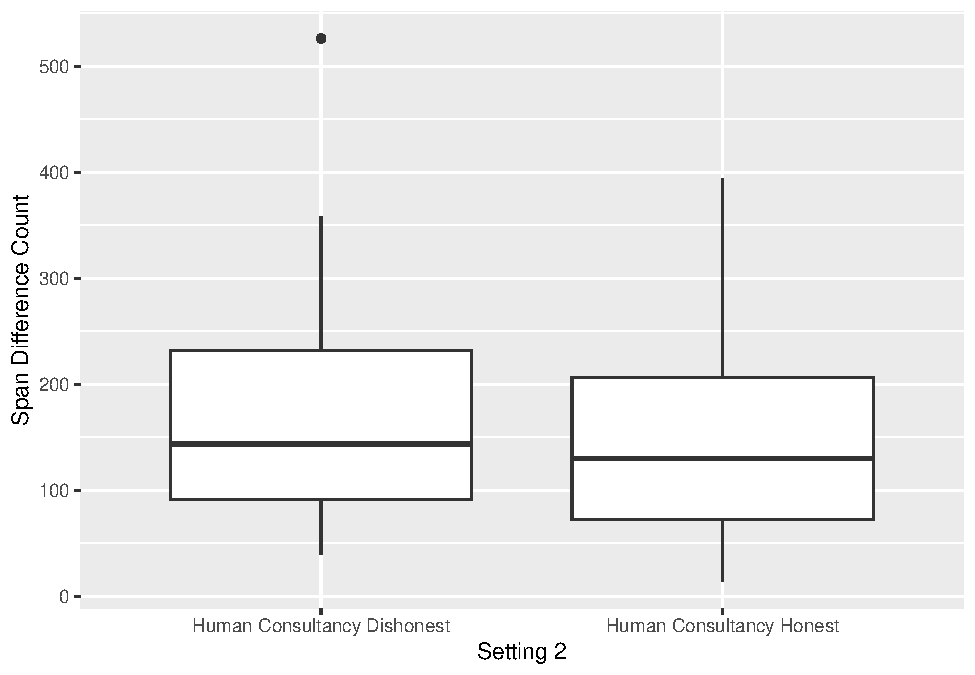
\includegraphics[width=1\linewidth]{debate-2309_files/figure-latex/quote_length graph-1}

\begin{Shaded}
\begin{Highlighting}[]
\NormalTok{filtered\_outliers }\OtherTok{\textless{}{-}}\NormalTok{ characters }\SpecialCharTok{\%\textgreater{}\%}
  \FunctionTok{group\_by}\NormalTok{(Final\_Setting) }\SpecialCharTok{\%\textgreater{}\%}
  \FunctionTok{mutate}\NormalTok{(}\AttributeTok{Q1 =} \FunctionTok{quantile}\NormalTok{(quote\_length, }\FloatTok{0.25}\NormalTok{),}
         \AttributeTok{Q3 =} \FunctionTok{quantile}\NormalTok{(quote\_length, }\FloatTok{0.75}\NormalTok{),}
         \AttributeTok{IQR =}\NormalTok{ Q3 }\SpecialCharTok{{-}}\NormalTok{ Q1,}
         \AttributeTok{lower\_bound =}\NormalTok{ Q1 }\SpecialCharTok{{-}} \FloatTok{1.5} \SpecialCharTok{*}\NormalTok{ IQR,}
         \AttributeTok{upper\_bound =}\NormalTok{ Q3 }\SpecialCharTok{+} \FloatTok{1.5} \SpecialCharTok{*}\NormalTok{ IQR)}

\FunctionTok{ggplot}\NormalTok{(characters) }\SpecialCharTok{+}
  \FunctionTok{geom\_boxplot}\NormalTok{(}\FunctionTok{aes}\NormalTok{(}\AttributeTok{x =}\NormalTok{ Final\_Setting, }\AttributeTok{y =} \StringTok{\textasciigrave{}}\AttributeTok{Quote length}\StringTok{\textasciigrave{}}\NormalTok{)) }\SpecialCharTok{+}
  \FunctionTok{labs}\NormalTok{(}\AttributeTok{y =} \StringTok{"Total Quote Length (characters)"}\NormalTok{)}\SpecialCharTok{+}
  \FunctionTok{theme\_minimal}\NormalTok{()}
\end{Highlighting}
\end{Shaded}

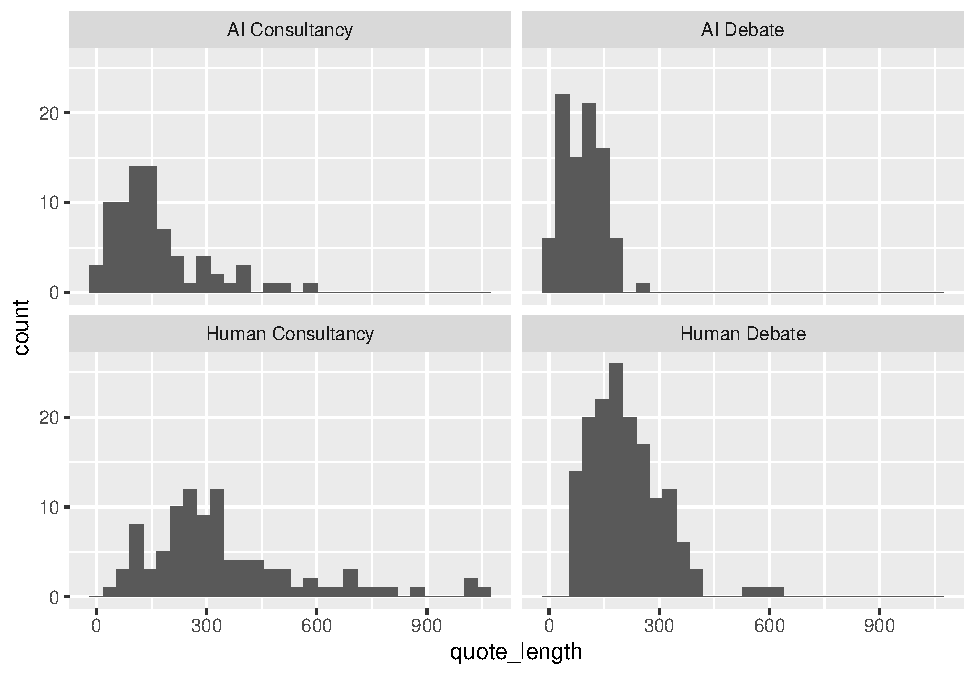
\includegraphics[width=1\linewidth]{debate-2309_files/figure-latex/quote_length graph-2}

\begin{Shaded}
\begin{Highlighting}[]
\NormalTok{filtered }\OtherTok{\textless{}{-}}\NormalTok{ characters }\SpecialCharTok{\%\textgreater{}\%}
  \FunctionTok{group\_by}\NormalTok{(Final\_Setting) }\SpecialCharTok{\%\textgreater{}\%}
  \FunctionTok{mutate}\NormalTok{(}\AttributeTok{Q1 =} \FunctionTok{quantile}\NormalTok{(quote\_length, }\FloatTok{0.25}\NormalTok{),}
         \AttributeTok{Q3 =} \FunctionTok{quantile}\NormalTok{(quote\_length, }\FloatTok{0.75}\NormalTok{),}
         \AttributeTok{IQR =}\NormalTok{ Q3 }\SpecialCharTok{{-}}\NormalTok{ Q1,}
         \AttributeTok{lower\_bound =}\NormalTok{ Q1 }\SpecialCharTok{{-}} \FloatTok{1.5} \SpecialCharTok{*}\NormalTok{ IQR,}
         \AttributeTok{upper\_bound =}\NormalTok{ Q3 }\SpecialCharTok{+} \FloatTok{1.5} \SpecialCharTok{*}\NormalTok{ IQR) }\SpecialCharTok{\%\textgreater{}\%}
  \FunctionTok{filter}\NormalTok{(quote\_length }\SpecialCharTok{\textgreater{}} \DecValTok{0} \SpecialCharTok{\&}\NormalTok{ quote\_length }\SpecialCharTok{\textless{}} \DecValTok{750}\NormalTok{) }\SpecialCharTok{\%\textgreater{}\%}
  \FunctionTok{select}\NormalTok{(}\SpecialCharTok{{-}}\NormalTok{Q1, }\SpecialCharTok{{-}}\NormalTok{Q3, }\SpecialCharTok{{-}}\NormalTok{IQR, }\SpecialCharTok{{-}}\NormalTok{lower\_bound, }\SpecialCharTok{{-}}\NormalTok{upper\_bound) }
\NormalTok{filtered }\SpecialCharTok{\%\textgreater{}\%}
  \FunctionTok{ggplot}\NormalTok{() }\SpecialCharTok{+}
  \FunctionTok{geom\_boxplot}\NormalTok{(}\FunctionTok{aes}\NormalTok{(}\AttributeTok{x =}\NormalTok{ Final\_Setting, }\AttributeTok{y =}\NormalTok{ quote\_length)) }\SpecialCharTok{+}
  \FunctionTok{labs}\NormalTok{(}\AttributeTok{y =} \StringTok{"Total Quote Length in a Debate/Consultancy (unique tokens)"}\NormalTok{, }\AttributeTok{x =} \StringTok{"Setting"}\NormalTok{)}\SpecialCharTok{+}
  \FunctionTok{theme\_minimal}\NormalTok{()}
\end{Highlighting}
\end{Shaded}

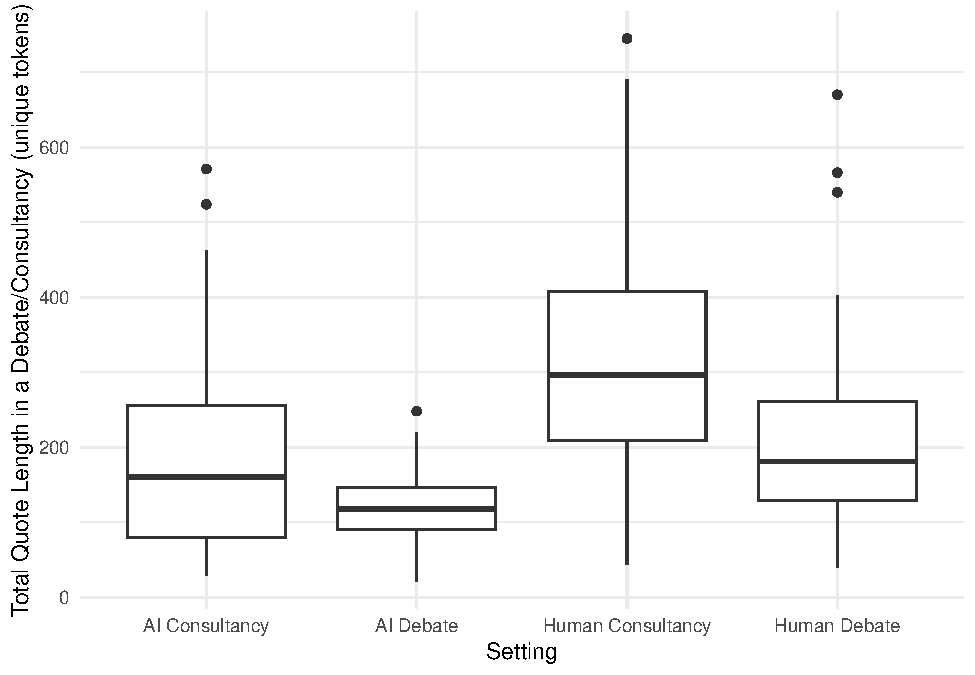
\includegraphics[width=1\linewidth]{debate-2309_files/figure-latex/quote_length graph-3}

\begin{Shaded}
\begin{Highlighting}[]
\NormalTok{characters }\SpecialCharTok{\%\textgreater{}\%}
  \FunctionTok{ggplot}\NormalTok{() }\SpecialCharTok{+}
  \FunctionTok{geom\_boxplot}\NormalTok{(}\FunctionTok{aes}\NormalTok{(}\AttributeTok{x =}\NormalTok{ Final\_Setting, }\AttributeTok{y =}\NormalTok{ quote\_length)) }\SpecialCharTok{+}
  \FunctionTok{labs}\NormalTok{(}\AttributeTok{y =} \StringTok{"Total Quote Length in a Debate/Consultancy (unique tokens)"}\NormalTok{, }\AttributeTok{x =} \StringTok{"Setting"}\NormalTok{)}\SpecialCharTok{+}
  \FunctionTok{theme\_minimal}\NormalTok{()}
\end{Highlighting}
\end{Shaded}

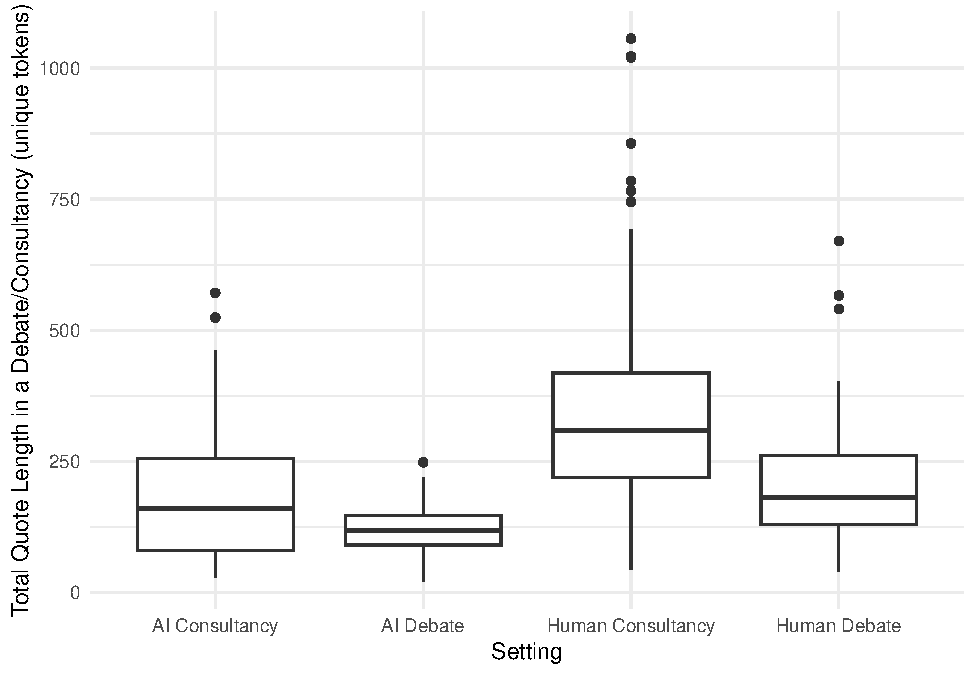
\includegraphics[width=1\linewidth]{debate-2309_files/figure-latex/quote_length graph-4}

\begin{Shaded}
\begin{Highlighting}[]
\FunctionTok{pairwise.t.test}\NormalTok{(filtered}\SpecialCharTok{$}\NormalTok{quote\_length, filtered}\SpecialCharTok{$}\NormalTok{Final\_Setting)}
\end{Highlighting}
\end{Shaded}

\begin{verbatim}
## 
##  Pairwise comparisons using t tests with pooled SD 
## 
## data:  filtered$quote_length and filtered$Final_Setting 
## 
##                   AI Consultancy AI Debate      Human Consultancy
## AI Debate         0.04290        -              -                
## Human Consultancy 0.00017        0.000000000018 -                
## Human Debate      0.80222        0.00443        0.000000019213   
## 
## P value adjustment method: holm
\end{verbatim}

\begin{Shaded}
\begin{Highlighting}[]
\NormalTok{filtered }\SpecialCharTok{\%\textgreater{}\%} \FunctionTok{group\_by}\NormalTok{(Final\_Setting) }\SpecialCharTok{\%\textgreater{}\%} \FunctionTok{summarise}\NormalTok{(}\AttributeTok{avground =} \FunctionTok{median}\NormalTok{(quote\_length))}
\end{Highlighting}
\end{Shaded}

\begin{verbatim}
## # A tibble: 4 x 2
##   Final_Setting     avground
##   <chr>                <dbl>
## 1 AI Consultancy        160 
## 2 AI Debate             118.
## 3 Human Consultancy     296 
## 4 Human Debate          181
\end{verbatim}

\begin{Shaded}
\begin{Highlighting}[]
\NormalTok{characters }\SpecialCharTok{\%\textgreater{}\%} \FunctionTok{group\_by}\NormalTok{(Final\_Setting) }\SpecialCharTok{\%\textgreater{}\%} \FunctionTok{summarise}\NormalTok{(}\AttributeTok{avground =} \FunctionTok{median}\NormalTok{(quote\_length))}
\end{Highlighting}
\end{Shaded}

\begin{verbatim}
## # A tibble: 4 x 2
##   Final_Setting     avground
##   <chr>                <dbl>
## 1 AI Consultancy        160 
## 2 AI Debate             118.
## 3 Human Consultancy     309 
## 4 Human Debate          181
\end{verbatim}

\begin{Shaded}
\begin{Highlighting}[]
\NormalTok{characters }\OtherTok{\textless{}{-}}\NormalTok{ characters }\SpecialCharTok{\%\textgreater{}\%}
  \FunctionTok{group\_by}\NormalTok{(}\StringTok{\textasciigrave{}}\AttributeTok{Room name}\StringTok{\textasciigrave{}}\NormalTok{,) }\SpecialCharTok{\%\textgreater{}\%}
  \FunctionTok{mutate}\NormalTok{(}\StringTok{\textasciigrave{}}\AttributeTok{Max judge rounds by room}\StringTok{\textasciigrave{}} \OtherTok{=} \FunctionTok{max}\NormalTok{(}\StringTok{\textasciigrave{}}\AttributeTok{Num previous judging rounds}\StringTok{\textasciigrave{}}\NormalTok{, }\AttributeTok{na.rm =} \ConstantTok{TRUE}\NormalTok{)) }\SpecialCharTok{\%\textgreater{}\%}
  \FunctionTok{ungroup}\NormalTok{()}
\FunctionTok{ggplot}\NormalTok{(characters) }\SpecialCharTok{+}
  \FunctionTok{geom\_boxplot}\NormalTok{(}\FunctionTok{aes}\NormalTok{(}\AttributeTok{x =}\NormalTok{ Final\_Setting, }\AttributeTok{y =} \StringTok{\textasciigrave{}}\AttributeTok{Max judge rounds by room}\StringTok{\textasciigrave{}}\NormalTok{)) }\SpecialCharTok{+}
  \FunctionTok{labs}\NormalTok{(}\AttributeTok{y =} \StringTok{\textquotesingle{}Max Judging Rounds\textquotesingle{}}\NormalTok{) }\SpecialCharTok{+}
  \FunctionTok{theme\_minimal}\NormalTok{() }
\end{Highlighting}
\end{Shaded}

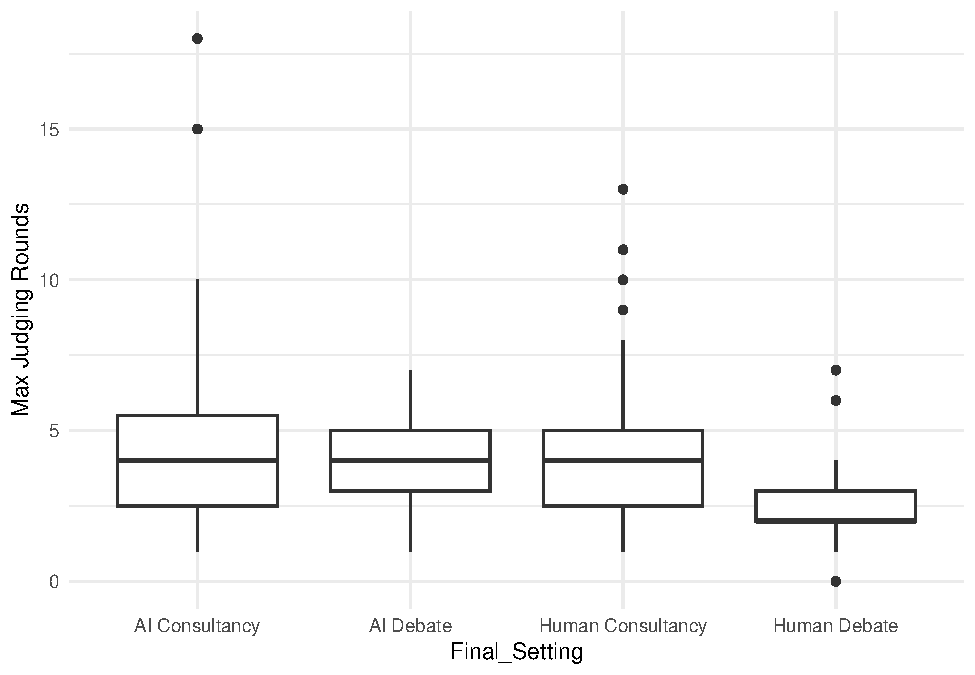
\includegraphics[width=1\linewidth]{debate-2309_files/figure-latex/rounds graph-1}

\begin{Shaded}
\begin{Highlighting}[]
\FunctionTok{pairwise.t.test}\NormalTok{(characters}\SpecialCharTok{$}\StringTok{\textasciigrave{}}\AttributeTok{Max judge rounds by room}\StringTok{\textasciigrave{}}\NormalTok{, characters}\SpecialCharTok{$}\NormalTok{Final\_Setting)}
\end{Highlighting}
\end{Shaded}

\begin{verbatim}
## 
##  Pairwise comparisons using t tests with pooled SD 
## 
## data:  characters$`Max judge rounds by room` and characters$Final_Setting 
## 
##                   AI Consultancy AI Debate Human Consultancy
## AI Debate         0.137          -         -                
## Human Consultancy 0.055          0.914     -                
## Human Debate      0.0000003      0.002     0.0000020        
## 
## P value adjustment method: holm
\end{verbatim}

\begin{Shaded}
\begin{Highlighting}[]
\NormalTok{filtered }\OtherTok{\textless{}{-}}\NormalTok{ characters }\SpecialCharTok{\%\textgreater{}\%}
  \FunctionTok{group\_by}\NormalTok{(Final\_Setting) }\SpecialCharTok{\%\textgreater{}\%}
  \FunctionTok{mutate}\NormalTok{(}\AttributeTok{Q1 =} \FunctionTok{quantile}\NormalTok{(}\StringTok{\textasciigrave{}}\AttributeTok{Max judge rounds by room}\StringTok{\textasciigrave{}}\NormalTok{, }\FloatTok{0.25}\NormalTok{),}
         \AttributeTok{Q3 =} \FunctionTok{quantile}\NormalTok{(}\StringTok{\textasciigrave{}}\AttributeTok{Max judge rounds by room}\StringTok{\textasciigrave{}}\NormalTok{, }\FloatTok{0.75}\NormalTok{),}
         \AttributeTok{IQR =}\NormalTok{ Q3 }\SpecialCharTok{{-}}\NormalTok{ Q1,}
         \AttributeTok{lower\_bound =}\NormalTok{ Q1 }\SpecialCharTok{{-}} \FloatTok{1.5} \SpecialCharTok{*}\NormalTok{ IQR,}
         \AttributeTok{upper\_bound =}\NormalTok{ Q3 }\SpecialCharTok{+} \FloatTok{1.5} \SpecialCharTok{*}\NormalTok{ IQR) }\SpecialCharTok{\%\textgreater{}\%}
  \FunctionTok{filter}\NormalTok{(}\StringTok{\textasciigrave{}}\AttributeTok{Max judge rounds by room}\StringTok{\textasciigrave{}} \SpecialCharTok{\textgreater{}=}\NormalTok{ lower\_bound }\SpecialCharTok{\&} \StringTok{\textasciigrave{}}\AttributeTok{Max judge rounds by room}\StringTok{\textasciigrave{}} \SpecialCharTok{\textless{}=}\NormalTok{ upper\_bound) }\SpecialCharTok{\%\textgreater{}\%}
  \FunctionTok{select}\NormalTok{(}\SpecialCharTok{{-}}\NormalTok{Q1, }\SpecialCharTok{{-}}\NormalTok{Q3, }\SpecialCharTok{{-}}\NormalTok{IQR, }\SpecialCharTok{{-}}\NormalTok{lower\_bound, }\SpecialCharTok{{-}}\NormalTok{upper\_bound)}
\NormalTok{filtered }\SpecialCharTok{\%\textgreater{}\%}
  \FunctionTok{ggplot}\NormalTok{() }\SpecialCharTok{+}
  \FunctionTok{geom\_boxplot}\NormalTok{(}\FunctionTok{aes}\NormalTok{(}\AttributeTok{x =}\NormalTok{ Final\_Setting, }\AttributeTok{y =} \StringTok{\textasciigrave{}}\AttributeTok{Max judge rounds by room}\StringTok{\textasciigrave{}}\NormalTok{), }\AttributeTok{outlier.shape =} \ConstantTok{NA}\NormalTok{) }\SpecialCharTok{+}
  \FunctionTok{labs}\NormalTok{(}\AttributeTok{y =} \StringTok{"Rounds"}\NormalTok{, }\AttributeTok{x =} \StringTok{"Setting"}\NormalTok{)}\SpecialCharTok{+}
  \FunctionTok{theme\_minimal}\NormalTok{()}
\end{Highlighting}
\end{Shaded}

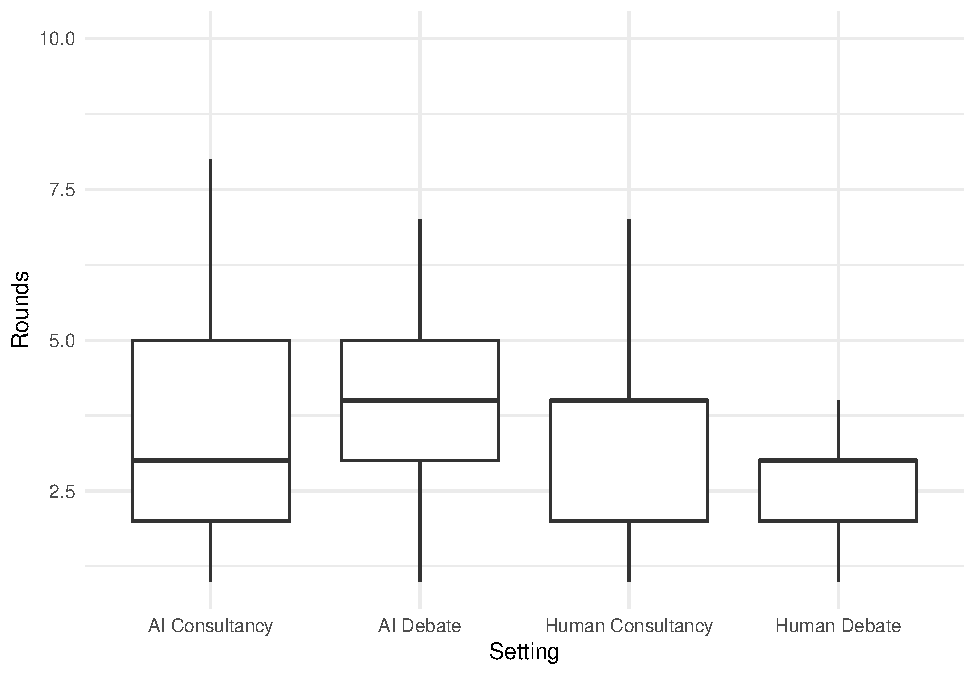
\includegraphics[width=1\linewidth]{debate-2309_files/figure-latex/rounds graph-2}

\begin{Shaded}
\begin{Highlighting}[]
\NormalTok{characters }\SpecialCharTok{\%\textgreater{}\%}
  \FunctionTok{ggplot}\NormalTok{() }\SpecialCharTok{+}
  \FunctionTok{geom\_boxplot}\NormalTok{(}\FunctionTok{aes}\NormalTok{(}\AttributeTok{x =}\NormalTok{ Final\_Setting, }\AttributeTok{y =} \StringTok{\textasciigrave{}}\AttributeTok{Max judge rounds by room}\StringTok{\textasciigrave{}}\NormalTok{)) }\SpecialCharTok{+}
  \FunctionTok{labs}\NormalTok{(}\AttributeTok{y =} \StringTok{"Rounds"}\NormalTok{, }\AttributeTok{x =} \StringTok{"Setting"}\NormalTok{)}\SpecialCharTok{+}
  \FunctionTok{theme\_minimal}\NormalTok{()}
\end{Highlighting}
\end{Shaded}

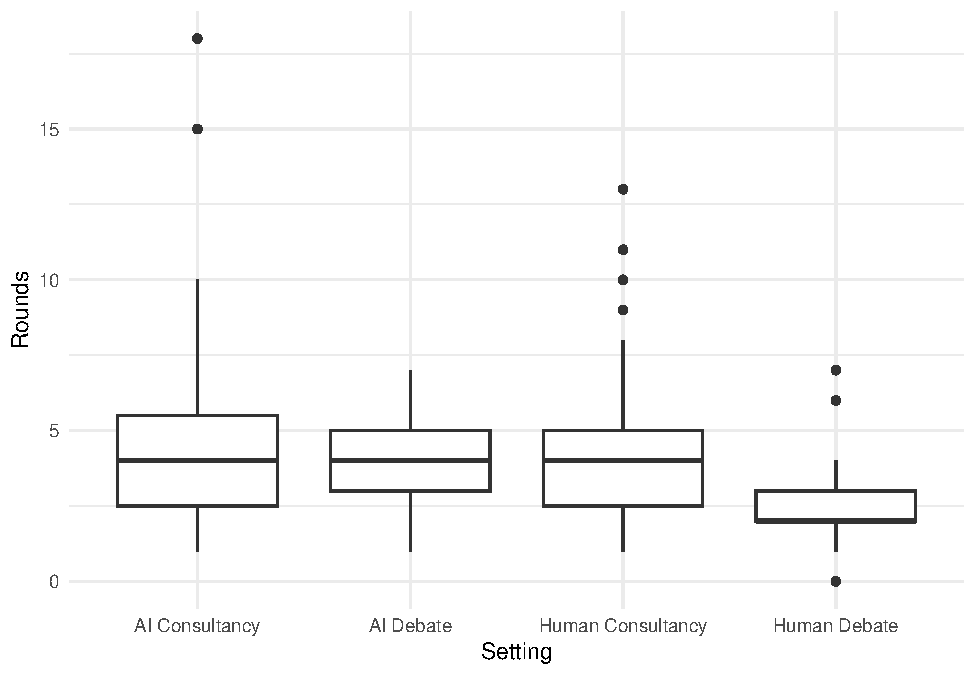
\includegraphics[width=1\linewidth]{debate-2309_files/figure-latex/rounds graph-3}

\begin{Shaded}
\begin{Highlighting}[]
\FunctionTok{pairwise.t.test}\NormalTok{(filtered}\SpecialCharTok{$}\NormalTok{quote\_length, filtered}\SpecialCharTok{$}\NormalTok{Final\_Setting)}
\end{Highlighting}
\end{Shaded}

\begin{verbatim}
## 
##  Pairwise comparisons using t tests with pooled SD 
## 
## data:  filtered$quote_length and filtered$Final_Setting 
## 
##                   AI Consultancy   AI Debate        Human Consultancy
## AI Debate         0.192            -                -                
## Human Consultancy 0.00000150627713 0.00000000000097 -                
## Human Debate      0.560            0.018            0.00000000003675 
## 
## P value adjustment method: holm
\end{verbatim}

\begin{Shaded}
\begin{Highlighting}[]
\NormalTok{filtered }\SpecialCharTok{\%\textgreater{}\%} \FunctionTok{group\_by}\NormalTok{(Final\_Setting) }\SpecialCharTok{\%\textgreater{}\%} \FunctionTok{summarise}\NormalTok{(}\AttributeTok{avground =} \FunctionTok{mean}\NormalTok{(}\StringTok{\textasciigrave{}}\AttributeTok{Max judge rounds by room}\StringTok{\textasciigrave{}}\NormalTok{))}
\end{Highlighting}
\end{Shaded}

\begin{verbatim}
## # A tibble: 4 x 2
##   Final_Setting     avground
##   <chr>                <dbl>
## 1 AI Consultancy        4.24
## 2 AI Debate             4.07
## 3 Human Consultancy     3.61
## 4 Human Debate          2.52
\end{verbatim}

\subsubsection{Length of debates,
stratified}\label{length-of-debates-stratified}

\begin{Shaded}
\begin{Highlighting}[]
\NormalTok{per\_turn }\OperatorTok{=}\NormalTok{ turns.merge(}
\NormalTok{        debates[[}\StringTok{"Room name"}\NormalTok{, }\StringTok{"Honest debater"}\NormalTok{, }\StringTok{"Dishonest debater"}\NormalTok{, }\StringTok{"Question"}\NormalTok{, }\StringTok{"Article ID"}\NormalTok{,}
                 \StringTok{"Speed annotator accuracy"}\NormalTok{,}\StringTok{"Untimed annotator context"}\NormalTok{,}\StringTok{"Untimed annotator context bins"}\NormalTok{,}\StringTok{"Is offline"}\NormalTok{,}\StringTok{"Final\_Setting"}\NormalTok{, }\StringTok{"Setting"}\NormalTok{,}\StringTok{"Final\_Accuracy"}\NormalTok{]],}
\NormalTok{        how}\OperatorTok{=}\StringTok{"left"}\NormalTok{,}
\NormalTok{        on}\OperatorTok{=}\StringTok{"Room name"}\NormalTok{,}
\NormalTok{    )}

\BuiltInTok{print}\NormalTok{(per\_turn.groupby(}\StringTok{\textquotesingle{}Final\_Setting\textquotesingle{}}\NormalTok{)[}\StringTok{\textquotesingle{}Num previous judging rounds\textquotesingle{}}\NormalTok{].mean())}
\end{Highlighting}
\end{Shaded}

\begin{verbatim}
## Final_Setting
## AI Consultancy       4.173252
## AI Debate            2.986231
## Human Consultancy    2.759310
## Human Debate         1.475072
## Name: Num previous judging rounds, dtype: float64
\end{verbatim}

\begin{Shaded}
\begin{Highlighting}[]
\CommentTok{\# Calculate the IQR and bounds for each group in \textquotesingle{}Setting 2\textquotesingle{}}
\NormalTok{grouped }\OperatorTok{=}\NormalTok{ per\_turn.groupby(}\StringTok{\textquotesingle{}Setting\textquotesingle{}}\NormalTok{)[}\StringTok{\textquotesingle{}Num previous judging rounds\textquotesingle{}}\NormalTok{]}

\NormalTok{Q1 }\OperatorTok{=}\NormalTok{ grouped.quantile(}\FloatTok{0.25}\NormalTok{)}
\NormalTok{Q3 }\OperatorTok{=}\NormalTok{ grouped.quantile(}\FloatTok{0.75}\NormalTok{)}
\NormalTok{IQR }\OperatorTok{=}\NormalTok{ Q3 }\OperatorTok{{-}}\NormalTok{ Q1}

\NormalTok{lower\_bound }\OperatorTok{=}\NormalTok{ Q1 }\OperatorTok{{-}} \FloatTok{1.5} \OperatorTok{*}\NormalTok{ IQR}
\NormalTok{upper\_bound }\OperatorTok{=}\NormalTok{ Q3 }\OperatorTok{+} \FloatTok{1.5} \OperatorTok{*}\NormalTok{ IQR}

\CommentTok{\# Filter out the outliers based on the computed bounds}
\NormalTok{filtered\_no\_outliers }\OperatorTok{=}\NormalTok{ per\_turn[}
\NormalTok{    (per\_turn[}\StringTok{\textquotesingle{}Setting\textquotesingle{}}\NormalTok{].}\BuiltInTok{map}\NormalTok{(lower\_bound) }\OperatorTok{\textless{}=}\NormalTok{ per\_turn[}\StringTok{\textquotesingle{}Num previous judging rounds\textquotesingle{}}\NormalTok{]) }\OperatorTok{\&}
\NormalTok{    (per\_turn[}\StringTok{\textquotesingle{}Setting\textquotesingle{}}\NormalTok{].}\BuiltInTok{map}\NormalTok{(upper\_bound) }\OperatorTok{\textgreater{}=}\NormalTok{ per\_turn[}\StringTok{\textquotesingle{}Num previous judging rounds\textquotesingle{}}\NormalTok{])}
\NormalTok{]}

\NormalTok{filtered\_no\_outliers}
\end{Highlighting}
\end{Shaded}

\begin{verbatim}
##                            Room name  ...  Final_Accuracy
## 0                         ambition-8  ...            True
## 1                         ambition-8  ...            True
## 2                         ambition-8  ...            True
## 3                         ambition-8  ...            True
## 4                         ambition-8  ...            True
## ...                              ...  ...             ...
## 6013                   break-a-leg-3  ...            True
## 6014                   break-a-leg-3  ...            True
## 6015  the-absurdity-of-family-love-2  ...            True
## 6016  the-absurdity-of-family-love-2  ...            True
## 6017  the-absurdity-of-family-love-2  ...            True
## 
## [5875 rows x 27 columns]
\end{verbatim}

\begin{Shaded}
\begin{Highlighting}[]
\ControlFlowTok{for}\NormalTok{ setting }\KeywordTok{in}\NormalTok{ filtered\_no\_outliers[}\StringTok{\textquotesingle{}Setting\textquotesingle{}}\NormalTok{].unique():}
\NormalTok{  per\_turn\_setting }\OperatorTok{=}\NormalTok{ filtered\_no\_outliers[filtered\_no\_outliers[}\StringTok{\textquotesingle{}Setting\textquotesingle{}}\NormalTok{]}\OperatorTok{==}\NormalTok{setting]}
  \BuiltInTok{print}\NormalTok{(setting)}
  \CommentTok{\# Calculate the maximum \textquotesingle{}Num previous judging rounds\textquotesingle{} for each combination of \textquotesingle{}Room name\textquotesingle{} and \textquotesingle{}Participant\textquotesingle{}}
\NormalTok{  per\_turn\_setting[}\StringTok{\textquotesingle{}Max judge rounds by room\textquotesingle{}}\NormalTok{] }\OperatorTok{=}\NormalTok{ per\_turn\_setting.groupby([}\StringTok{\textquotesingle{}Room name\textquotesingle{}}\NormalTok{, }\StringTok{\textquotesingle{}Participant\textquotesingle{}}\NormalTok{])[}\StringTok{\textquotesingle{}Num previous judging rounds\textquotesingle{}}\NormalTok{].transform(}\StringTok{\textquotesingle{}max\textquotesingle{}}\NormalTok{)}
  \CommentTok{\#\# Just based on the number of rounds}
  
  \ControlFlowTok{for}\NormalTok{ i }\KeywordTok{in} \BuiltInTok{range}\NormalTok{(}\DecValTok{1}\NormalTok{, per\_turn\_setting[}\StringTok{\textquotesingle{}Max judge rounds by room\textquotesingle{}}\NormalTok{].}\BuiltInTok{max}\NormalTok{() }\OperatorTok{+} \DecValTok{1}\NormalTok{):}
\NormalTok{      max\_rounds }\OperatorTok{=}\NormalTok{ per\_turn\_setting[(per\_turn\_setting[}\StringTok{\textquotesingle{}Max judge rounds by room\textquotesingle{}}\NormalTok{] }\OperatorTok{==}\NormalTok{ i) }\OperatorTok{\&}\NormalTok{ (per\_turn\_setting[}\StringTok{\textquotesingle{}Untimed annotator context\textquotesingle{}}\NormalTok{] }\OperatorTok{\textgreater{}} \DecValTok{0}\NormalTok{)]}
      \BuiltInTok{print}\NormalTok{(}\BuiltInTok{len}\NormalTok{(max\_rounds))}
      \CommentTok{\# Group by \textquotesingle{}Num previous judging rounds\textquotesingle{} and calculate the mean of \textquotesingle{}Probability correct\textquotesingle{}}
\NormalTok{      average\_pc\_per\_round }\OperatorTok{=}\NormalTok{ max\_rounds.groupby(}\StringTok{\textquotesingle{}Num previous judging rounds\textquotesingle{}}\NormalTok{)[}\StringTok{\textquotesingle{}Probability correct\textquotesingle{}}\NormalTok{].mean()}
  
      \CommentTok{\# Create a new DataFrame with \textquotesingle{}Num previous judging rounds\textquotesingle{} and \textquotesingle{}Average pc per round\textquotesingle{}}
\NormalTok{      probability\_correct\_round }\OperatorTok{=}\NormalTok{ pd.DataFrame(\{}\StringTok{\textquotesingle{}Num previous judging rounds\textquotesingle{}}\NormalTok{: average\_pc\_per\_round.index,}
                                                \StringTok{\textquotesingle{}Average pc per round\textquotesingle{}}\NormalTok{: average\_pc\_per\_round.values\})}
  
      \CommentTok{\# Plotting the data with label for the line}
\NormalTok{      plt.plot(probability\_correct\_round[}\StringTok{\textquotesingle{}Num previous judging rounds\textquotesingle{}}\NormalTok{], probability\_correct\_round[}\StringTok{\textquotesingle{}Average pc per round\textquotesingle{}}\NormalTok{], label}\OperatorTok{=}\SpecialStringTok{f"Max Rounds: }\SpecialCharTok{\{}\NormalTok{i}\SpecialCharTok{\}}\SpecialStringTok{"}\NormalTok{)}
  
\NormalTok{  plt.title(}\SpecialStringTok{f"Probability Correct for Setting: }\SpecialCharTok{\{}\NormalTok{setting}\SpecialCharTok{\}}\SpecialStringTok{"}\NormalTok{) }
\NormalTok{  plt.xlabel(}\StringTok{\textquotesingle{}Num previous judging rounds\textquotesingle{}}\NormalTok{)}
\NormalTok{  plt.ylabel(}\StringTok{\textquotesingle{}Average pc per round\textquotesingle{}}\NormalTok{)}
\NormalTok{  plt.legend()}
\NormalTok{  plt.show()}
\end{Highlighting}
\end{Shaded}

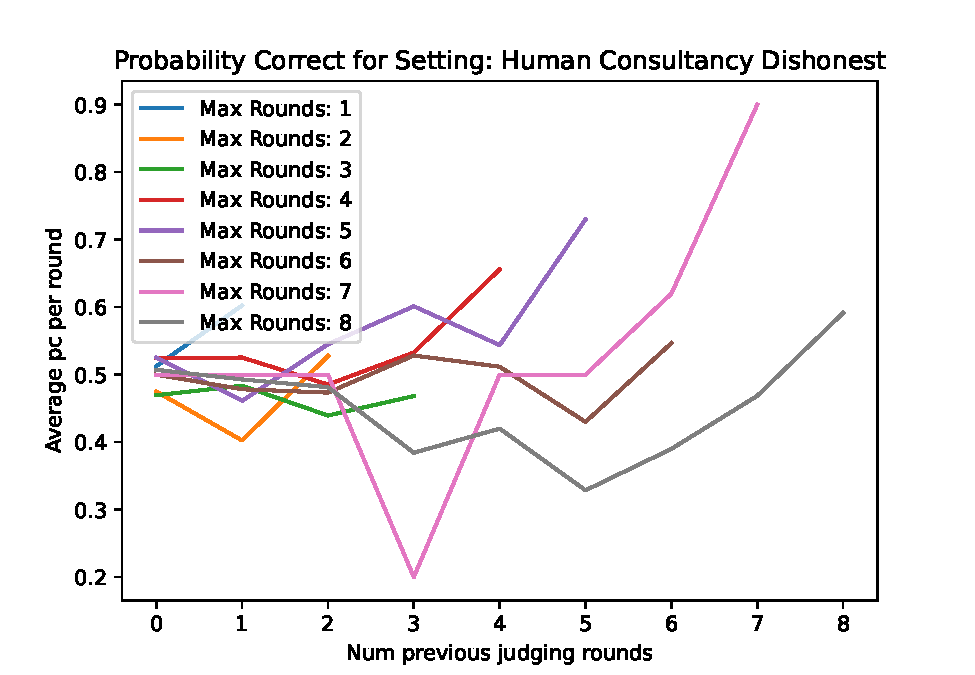
\includegraphics[width=1\linewidth]{debate-2309_files/figure-latex/strat-1}
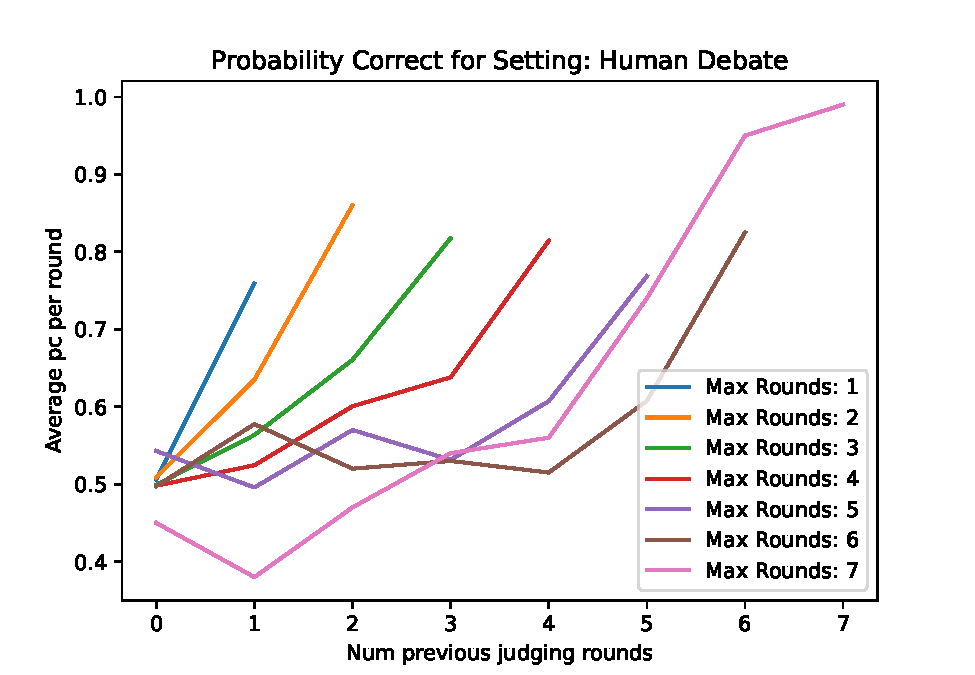
\includegraphics[width=1\linewidth]{debate-2309_files/figure-latex/strat-2}
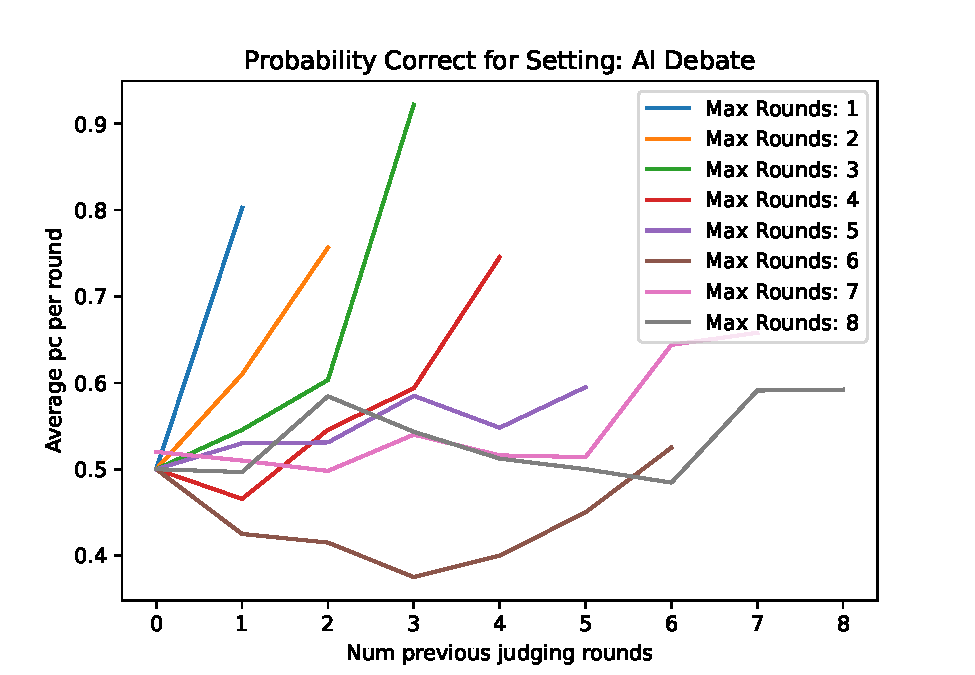
\includegraphics[width=1\linewidth]{debate-2309_files/figure-latex/strat-3}
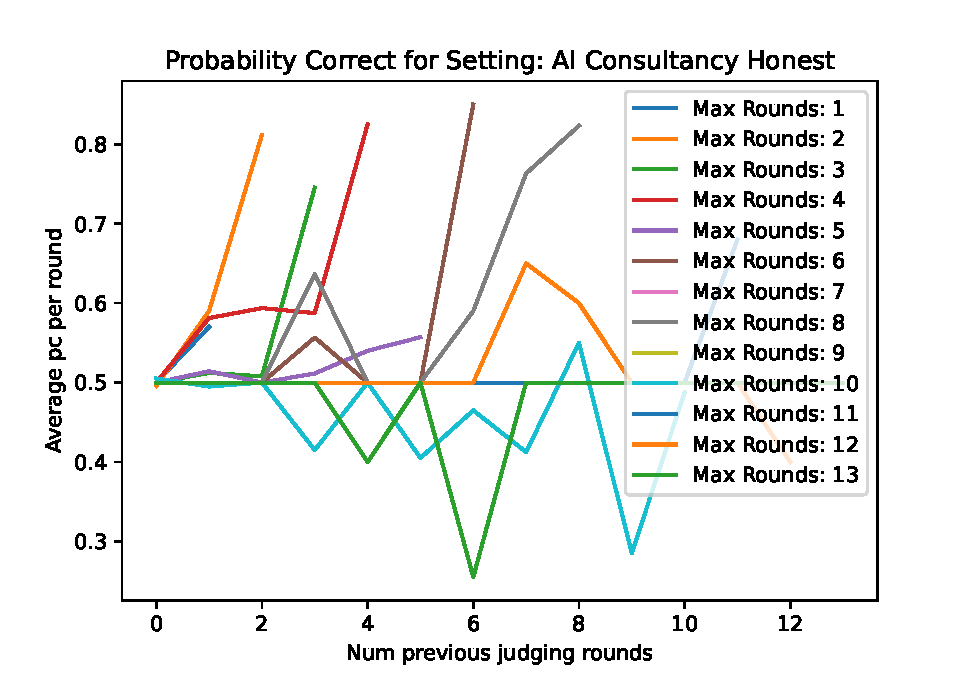
\includegraphics[width=1\linewidth]{debate-2309_files/figure-latex/strat-4}
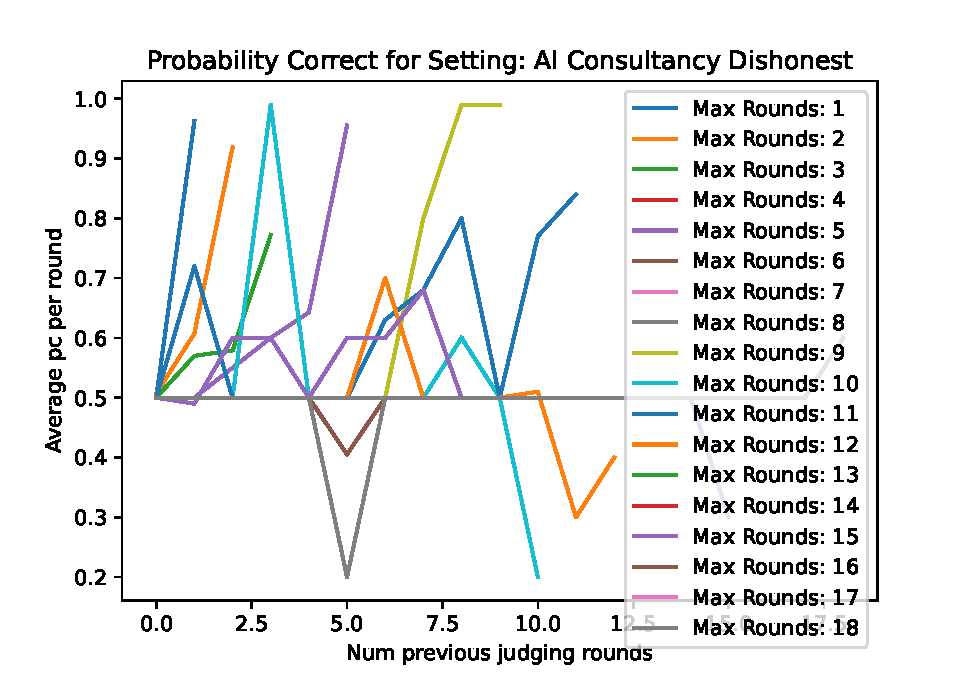
\includegraphics[width=1\linewidth]{debate-2309_files/figure-latex/strat-5}
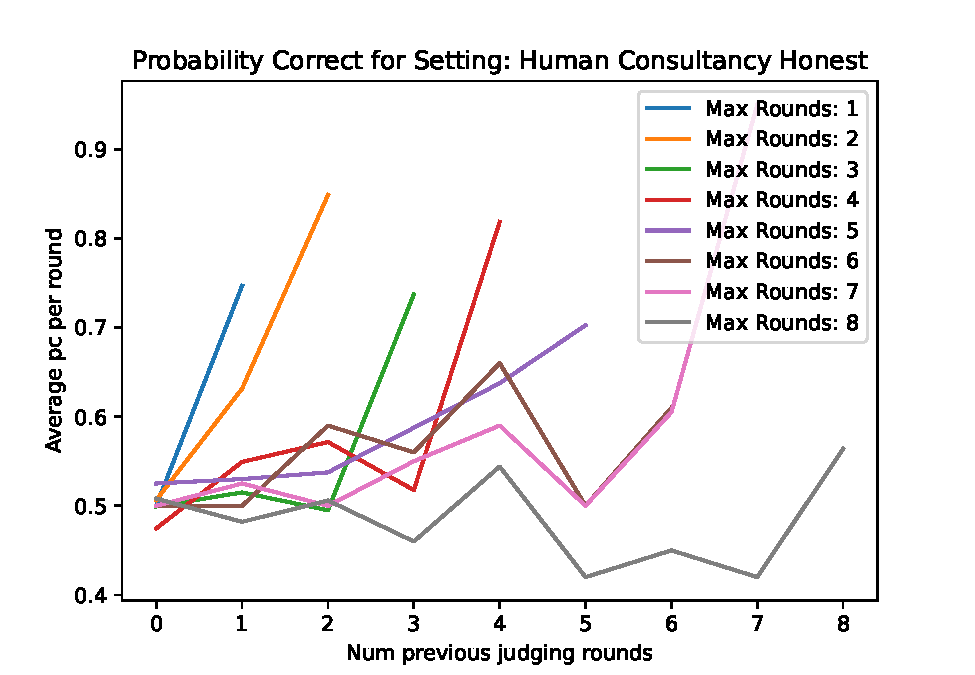
\includegraphics[width=1\linewidth]{debate-2309_files/figure-latex/strat-6}

\begin{Shaded}
\begin{Highlighting}[]
\NormalTok{strat }\OtherTok{\textless{}{-}}\NormalTok{ py}\SpecialCharTok{$}\NormalTok{per\_turn}
\NormalTok{strat }\OtherTok{\textless{}{-}}\NormalTok{ strat }\SpecialCharTok{\%\textgreater{}\%}
  \FunctionTok{group\_by}\NormalTok{(}\StringTok{\textasciigrave{}}\AttributeTok{Room name}\StringTok{\textasciigrave{}}\NormalTok{, Participant) }\SpecialCharTok{\%\textgreater{}\%}
  \FunctionTok{mutate}\NormalTok{(}\StringTok{\textasciigrave{}}\AttributeTok{Max judge rounds by room}\StringTok{\textasciigrave{}} \OtherTok{=} \FunctionTok{max}\NormalTok{(}\StringTok{\textasciigrave{}}\AttributeTok{Num previous judging rounds}\StringTok{\textasciigrave{}}\NormalTok{, }\AttributeTok{na.rm =} \ConstantTok{TRUE}\NormalTok{)) }\SpecialCharTok{\%\textgreater{}\%}
  \FunctionTok{ungroup}\NormalTok{()}
\NormalTok{strat }\OtherTok{\textless{}{-}}\NormalTok{ strat }\SpecialCharTok{\%\textgreater{}\%}
  \FunctionTok{mutate}\NormalTok{(}\StringTok{\textasciigrave{}}\AttributeTok{Max judge rounds bin}\StringTok{\textasciigrave{}} \OtherTok{=} \FunctionTok{cut}\NormalTok{(}\StringTok{\textasciigrave{}}\AttributeTok{Max judge rounds by room}\StringTok{\textasciigrave{}}\NormalTok{, }
                                      \AttributeTok{breaks =} \FunctionTok{seq}\NormalTok{(}\DecValTok{0}\NormalTok{, }\FunctionTok{max}\NormalTok{(}\StringTok{\textasciigrave{}}\AttributeTok{Max judge rounds by room}\StringTok{\textasciigrave{}}\NormalTok{, }\AttributeTok{na.rm =} \ConstantTok{TRUE}\NormalTok{) }\SpecialCharTok{+} \DecValTok{3}\NormalTok{, }\AttributeTok{by =} \DecValTok{3}\NormalTok{), }
                                      \AttributeTok{labels =} \ConstantTok{FALSE}\NormalTok{, }
                                      \AttributeTok{include.lowest =} \ConstantTok{TRUE}\NormalTok{, }
                                      \AttributeTok{right =} \ConstantTok{FALSE}\NormalTok{))}

\CommentTok{\# Plot using ggplot2}
\NormalTok{strat }\SpecialCharTok{\%\textgreater{}\%}
  \FunctionTok{group\_by}\NormalTok{(Setting, }\StringTok{\textasciigrave{}}\AttributeTok{Num previous judging rounds}\StringTok{\textasciigrave{}}\NormalTok{, }\StringTok{\textasciigrave{}}\AttributeTok{Max judge rounds bin}\StringTok{\textasciigrave{}}\NormalTok{) }\SpecialCharTok{\%\textgreater{}\%}
  \FunctionTok{summarize}\NormalTok{(}
    \StringTok{\textasciigrave{}}\AttributeTok{Average Probability Correct}\StringTok{\textasciigrave{}} \OtherTok{=} \FunctionTok{mean}\NormalTok{(}\StringTok{\textasciigrave{}}\AttributeTok{Probability correct}\StringTok{\textasciigrave{}}\NormalTok{, }\AttributeTok{na.rm =} \ConstantTok{TRUE}\NormalTok{),}
    \AttributeTok{n =} \FunctionTok{n}\NormalTok{(),}
    \AttributeTok{se =} \FunctionTok{sqrt}\NormalTok{(}\StringTok{\textasciigrave{}}\AttributeTok{Average Probability Correct}\StringTok{\textasciigrave{}} \SpecialCharTok{*}\NormalTok{ (}\DecValTok{1} \SpecialCharTok{{-}} \StringTok{\textasciigrave{}}\AttributeTok{Average Probability Correct}\StringTok{\textasciigrave{}}\NormalTok{) }\SpecialCharTok{/}\NormalTok{ n)}
\NormalTok{  ) }\SpecialCharTok{\%\textgreater{}\%}
  \FunctionTok{mutate}\NormalTok{(}
    \AttributeTok{lower\_ci =} \StringTok{\textasciigrave{}}\AttributeTok{Average Probability Correct}\StringTok{\textasciigrave{}} \SpecialCharTok{{-}} \FloatTok{1.96} \SpecialCharTok{*}\NormalTok{ se,}
    \AttributeTok{upper\_ci =} \StringTok{\textasciigrave{}}\AttributeTok{Average Probability Correct}\StringTok{\textasciigrave{}} \SpecialCharTok{+} \FloatTok{1.96} \SpecialCharTok{*}\NormalTok{ se}
\NormalTok{  ) }\SpecialCharTok{\%\textgreater{}\%}
  \FunctionTok{ggplot}\NormalTok{(}\FunctionTok{aes}\NormalTok{(}\AttributeTok{x =} \StringTok{\textasciigrave{}}\AttributeTok{Num previous judging rounds}\StringTok{\textasciigrave{}}\NormalTok{, }\AttributeTok{y =} \StringTok{\textasciigrave{}}\AttributeTok{Average Probability Correct}\StringTok{\textasciigrave{}}\NormalTok{, }\AttributeTok{col =} \FunctionTok{as.factor}\NormalTok{(}\StringTok{\textasciigrave{}}\AttributeTok{Max judge rounds bin}\StringTok{\textasciigrave{}}\NormalTok{))) }\SpecialCharTok{+}
  \FunctionTok{geom\_ribbon}\NormalTok{(}\FunctionTok{aes}\NormalTok{(}\AttributeTok{ymin =}\NormalTok{ lower\_ci, }\AttributeTok{ymax =}\NormalTok{ upper\_ci, }\AttributeTok{fill =} \FunctionTok{as.factor}\NormalTok{(}\StringTok{\textasciigrave{}}\AttributeTok{Max judge rounds bin}\StringTok{\textasciigrave{}}\NormalTok{), }\AttributeTok{group =} \FunctionTok{as.factor}\NormalTok{(}\StringTok{\textasciigrave{}}\AttributeTok{Max judge rounds bin}\StringTok{\textasciigrave{}}\NormalTok{), }\AttributeTok{color =} \ConstantTok{NULL}\NormalTok{), }\AttributeTok{alpha =} \FloatTok{0.15}\NormalTok{) }\SpecialCharTok{+}
  \FunctionTok{labs}\NormalTok{(}\AttributeTok{title =} \StringTok{"Average Probability Correct Each Round, }\SpecialCharTok{\textbackslash{}n}\StringTok{stratified by Max Round Binned"}\NormalTok{,}
       \AttributeTok{x =} \StringTok{"Round"}\NormalTok{, }
       \AttributeTok{y =} \StringTok{"Average Intermediate Probability Correct"}\NormalTok{) }\SpecialCharTok{+}
  \FunctionTok{geom\_line}\NormalTok{() }\SpecialCharTok{+}
  \FunctionTok{facet\_wrap}\NormalTok{(}\SpecialCharTok{\textasciitilde{}}\NormalTok{Setting) }\SpecialCharTok{+}
  \FunctionTok{theme\_bw}\NormalTok{() }\SpecialCharTok{+}
  \FunctionTok{theme}\NormalTok{(}\AttributeTok{legend.position =} \StringTok{"none"}\NormalTok{)}
\end{Highlighting}
\end{Shaded}

\begin{verbatim}
## `summarise()` has grouped output by 'Setting', 'Num previous judging rounds'.
## You can override using the `.groups` argument.
\end{verbatim}

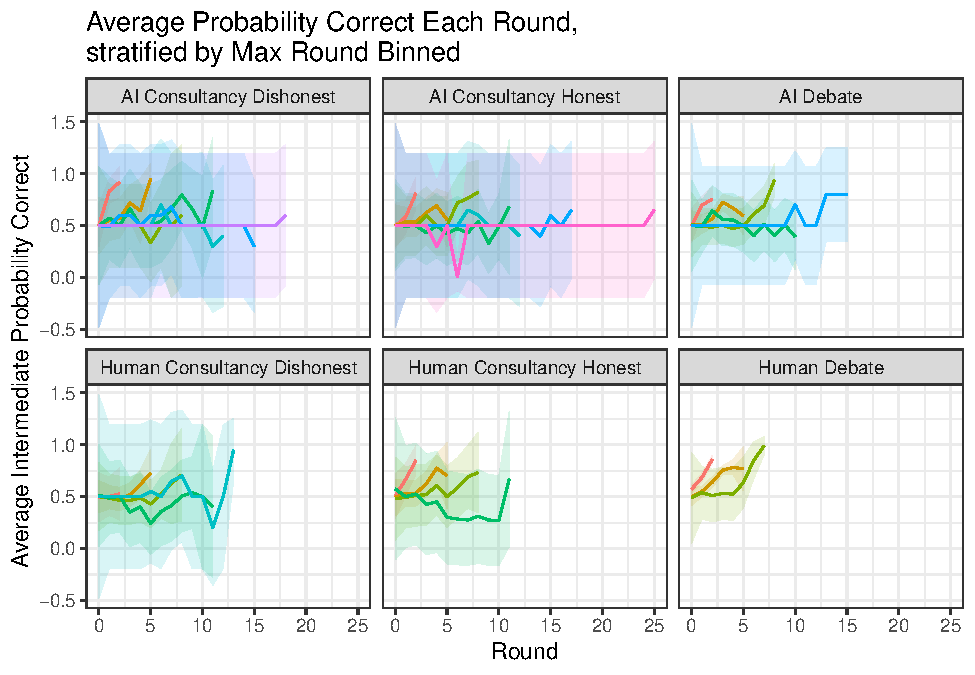
\includegraphics{debate-2309_files/figure-latex/strat ggplot-13.pdf}

\begin{Shaded}
\begin{Highlighting}[]
\NormalTok{strat }\SpecialCharTok{\%\textgreater{}\%}
  \FunctionTok{group\_by}\NormalTok{(Setting, }\StringTok{\textasciigrave{}}\AttributeTok{Num previous judging rounds}\StringTok{\textasciigrave{}}\NormalTok{, }\StringTok{\textasciigrave{}}\AttributeTok{Max judge rounds by room}\StringTok{\textasciigrave{}}\NormalTok{) }\SpecialCharTok{\%\textgreater{}\%}
  \FunctionTok{summarize}\NormalTok{(}\StringTok{\textasciigrave{}}\AttributeTok{Average Probability Correct}\StringTok{\textasciigrave{}} \OtherTok{=} \FunctionTok{mean}\NormalTok{(}\StringTok{\textasciigrave{}}\AttributeTok{Probability correct}\StringTok{\textasciigrave{}}\NormalTok{, }\AttributeTok{na.rm =} \ConstantTok{TRUE}\NormalTok{)) }\SpecialCharTok{\%\textgreater{}\%}
  \FunctionTok{mutate}\NormalTok{(}\AttributeTok{Completion =} \StringTok{\textasciigrave{}}\AttributeTok{Num previous judging rounds}\StringTok{\textasciigrave{}} \SpecialCharTok{/} \StringTok{\textasciigrave{}}\AttributeTok{Max judge rounds by room}\StringTok{\textasciigrave{}}\NormalTok{) }\SpecialCharTok{\%\textgreater{}\%}
  \FunctionTok{ggplot}\NormalTok{(}\FunctionTok{aes}\NormalTok{(}\AttributeTok{x =}\NormalTok{ Completion, }\AttributeTok{y =} \StringTok{\textasciigrave{}}\AttributeTok{Average Probability Correct}\StringTok{\textasciigrave{}}\NormalTok{, }\AttributeTok{col =} \FunctionTok{as.factor}\NormalTok{(}\StringTok{\textasciigrave{}}\AttributeTok{Max judge rounds by room}\StringTok{\textasciigrave{}}\NormalTok{), }\AttributeTok{group =} \FunctionTok{as.factor}\NormalTok{(}\StringTok{\textasciigrave{}}\AttributeTok{Max judge rounds by room}\StringTok{\textasciigrave{}}\NormalTok{))) }\SpecialCharTok{+}
  \FunctionTok{geom\_line}\NormalTok{() }\SpecialCharTok{+}
  \FunctionTok{labs}\NormalTok{(}\AttributeTok{title =} \StringTok{"Average Probability Correct by Percentage of Completion"}\NormalTok{,}
       \AttributeTok{x =} \StringTok{"Percentage of Completion"}\NormalTok{, }
       \AttributeTok{y =} \StringTok{"Average Probability Correct"}\NormalTok{) }\SpecialCharTok{+}
  \FunctionTok{facet\_wrap}\NormalTok{(}\SpecialCharTok{\textasciitilde{}}\NormalTok{Setting) }\SpecialCharTok{+}
  \FunctionTok{theme\_minimal}\NormalTok{() }\SpecialCharTok{+}
  \FunctionTok{theme}\NormalTok{(}\AttributeTok{legend.position =} \StringTok{"none"}\NormalTok{)}
\end{Highlighting}
\end{Shaded}

\begin{verbatim}
## `summarise()` has grouped output by 'Setting', 'Num previous judging rounds'.
## You can override using the `.groups` argument.
\end{verbatim}

\begin{verbatim}
## Warning: Removed 10 rows containing missing values (`geom_line()`).
\end{verbatim}

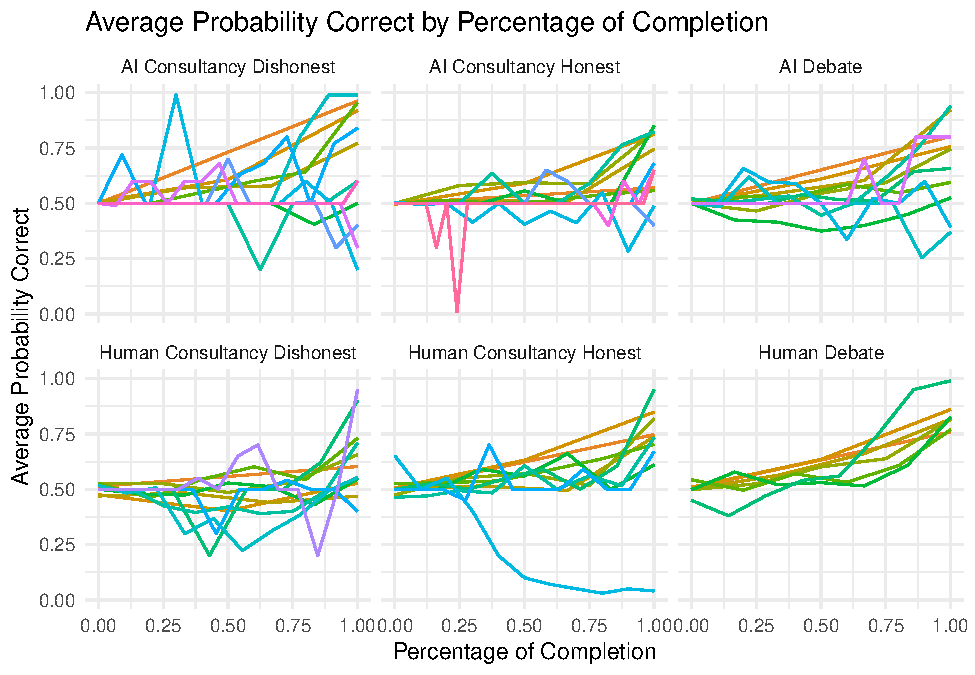
\includegraphics{debate-2309_files/figure-latex/strat ggplot-14.pdf}

\subsubsection{Time (offline judging..?)}\label{time-offline-judging..}

\begin{Shaded}
\begin{Highlighting}[]
\CommentTok{\# Convert to datetime}
\NormalTok{judgments[}\StringTok{"Offline judging start time"}\NormalTok{] }\OperatorTok{=}\NormalTok{ pd.to\_datetime(judgments[}\StringTok{"Offline judging start time"}\NormalTok{], unit}\OperatorTok{=}\StringTok{"ms"}\NormalTok{)}
\NormalTok{judgments[}\StringTok{"Offline judging end time"}\NormalTok{] }\OperatorTok{=}\NormalTok{ pd.to\_datetime(judgments[}\StringTok{"Offline judging end time"}\NormalTok{], unit}\OperatorTok{=}\StringTok{"ms"}\NormalTok{)}

\CommentTok{\# Calculate offline judging time in minutes}
\NormalTok{judgments[}\StringTok{"Offline judging time"}\NormalTok{] }\OperatorTok{=}\NormalTok{ (judgments[}\StringTok{"Offline judging end time"}\NormalTok{] }\OperatorTok{{-}}\NormalTok{ judgments[}\StringTok{"Offline judging start time"}\NormalTok{]).dt.total\_seconds() }\OperatorTok{/} \DecValTok{60}


\BuiltInTok{print}\NormalTok{(}\SpecialStringTok{f"Number of offline judgments on consultancies:}\CharTok{\textbackslash{}n}\SpecialCharTok{\{}\NormalTok{judgments[judgments[}\StringTok{\textquotesingle{}Setting\textquotesingle{}}\NormalTok{].}\BuiltInTok{str}\NormalTok{.contains(}\StringTok{\textquotesingle{}Consultancy\textquotesingle{}}\NormalTok{)][}\StringTok{\textquotesingle{}Offline judging time\textquotesingle{}}\NormalTok{]}\SpecialCharTok{.}\NormalTok{dropna()}\SpecialCharTok{.}\NormalTok{describe()}\SpecialCharTok{\}}\CharTok{\textbackslash{}n}\SpecialStringTok{Only 13..."}\NormalTok{)}
\end{Highlighting}
\end{Shaded}

\begin{verbatim}
## Number of offline judgments on consultancies:
## count      13.000000
## mean      447.514203
## std      1236.792144
## min         1.169167
## 25%         1.836600
## 50%         5.664767
## 75%        13.967783
## max      4369.697933
## Name: Offline judging time, dtype: float64
## Only 13...
\end{verbatim}

\begin{Shaded}
\begin{Highlighting}[]
\CommentTok{\# Filter out rows with NaT values}
\NormalTok{valid\_judging\_time }\OperatorTok{=}\NormalTok{ judgments[}\StringTok{"Offline judging time"}\NormalTok{].dropna()}

\CommentTok{\# Calculate summary statistics}
\NormalTok{summary\_stats }\OperatorTok{=}\NormalTok{ valid\_judging\_time.describe()}
\BuiltInTok{print}\NormalTok{(summary\_stats)}
\end{Highlighting}
\end{Shaded}

\begin{verbatim}
## count      203.000000
## mean       255.826710
## std       1372.208730
## min          0.667467
## 25%          2.867950
## 50%          5.176250
## 75%         10.295583
## max      14202.493917
## Name: Offline judging time, dtype: float64
\end{verbatim}

\begin{Shaded}
\begin{Highlighting}[]
\CommentTok{\# Filter judgments with offline judging time above 65 minutes}
\NormalTok{filtered\_judgments }\OperatorTok{=}\NormalTok{ judgments[(judgments[}\StringTok{"Offline judging time"}\NormalTok{] }\OperatorTok{\textless{}} \DecValTok{65}\NormalTok{) }\OperatorTok{\&}\NormalTok{ (judgments[}\StringTok{"Untimed annotator context"}\NormalTok{] }\OperatorTok{\textgreater{}} \DecValTok{0}\NormalTok{)]}

\CommentTok{\# Print filtered judgments}
\CommentTok{\# print("Filtered judgments with offline judging time above 65 minutes:")}
\BuiltInTok{print}\NormalTok{(filtered\_judgments[}\StringTok{\textquotesingle{}Offline judging time\textquotesingle{}}\NormalTok{].describe())}
\end{Highlighting}
\end{Shaded}

\begin{verbatim}
## count    193.000000
## mean       8.013787
## std        9.410150
## min        0.667467
## 25%        2.850450
## 50%        5.107450
## 75%        8.716300
## max       64.173267
## Name: Offline judging time, dtype: float64
\end{verbatim}

\begin{Shaded}
\begin{Highlighting}[]
\CommentTok{\# Create the histogram}
\NormalTok{plt.hist(filtered\_judgments[}\StringTok{\textquotesingle{}Offline judging time\textquotesingle{}}\NormalTok{], bins}\OperatorTok{=}\DecValTok{10}\NormalTok{)}

\CommentTok{\# Set labels and title}
\NormalTok{plt.xlabel(}\StringTok{"Offline Judging Time (minutes)"}\NormalTok{)}
\NormalTok{plt.ylabel(}\StringTok{"Frequency"}\NormalTok{)}
\NormalTok{plt.title(}\StringTok{"Histogram of Offline Judging Time"}\NormalTok{)}

\CommentTok{\# Display the histogram}
\NormalTok{plt.show()}
\end{Highlighting}
\end{Shaded}

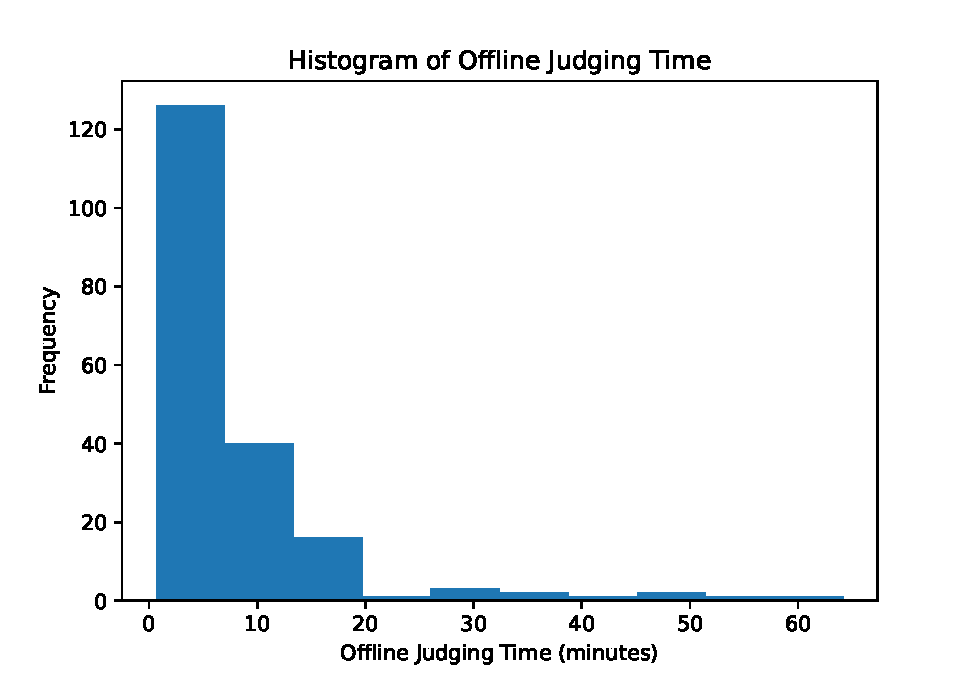
\includegraphics{debate-2309_files/figure-latex/TODO offline judging-1.pdf}

\begin{Shaded}
\begin{Highlighting}[]

\NormalTok{aggregates }\OperatorTok{=}\NormalTok{ \{}
    \StringTok{\textquotesingle{}Final probability correct\textquotesingle{}}\NormalTok{: }\StringTok{\textquotesingle{}mean\textquotesingle{}}\NormalTok{,}
    \StringTok{\textquotesingle{}Untimed annotator context\textquotesingle{}}\NormalTok{: }\StringTok{\textquotesingle{}mean\textquotesingle{}}
\NormalTok{\}}
\NormalTok{filtered\_judgments }\OperatorTok{=}\NormalTok{ filtered\_judgments.groupby(}\StringTok{\textquotesingle{}Offline judging time\textquotesingle{}}\NormalTok{).agg(aggregates).reset\_index()}
\end{Highlighting}
\end{Shaded}

\section{Analysis}\label{analysis}

\subsection{Question Difficulty}\label{question-difficulty}

confounder rounds, quotes

\begin{Shaded}
\begin{Highlighting}[]
\NormalTok{judgments[}\StringTok{"Number of judge continues bins"}\NormalTok{] }\OperatorTok{=}\NormalTok{ pd.cut(}
\NormalTok{    judgments[}\StringTok{"Number of judge continues"}\NormalTok{], }
\NormalTok{    bins}\OperatorTok{=}\NormalTok{[}\DecValTok{0}\NormalTok{, }\DecValTok{3}\NormalTok{, }\DecValTok{6}\NormalTok{, }\DecValTok{9}\NormalTok{, }\BuiltInTok{float}\NormalTok{(}\StringTok{\textquotesingle{}inf\textquotesingle{}}\NormalTok{)],  }\CommentTok{\# bin edges}
\NormalTok{    labels}\OperatorTok{=}\NormalTok{[}\StringTok{\textquotesingle{}1{-}3\textquotesingle{}}\NormalTok{, }\StringTok{\textquotesingle{}4{-}6\textquotesingle{}}\NormalTok{, }\StringTok{\textquotesingle{}7{-}9\textquotesingle{}}\NormalTok{, }\StringTok{\textquotesingle{}10+\textquotesingle{}}\NormalTok{],  }\CommentTok{\# labels for the resulting bins}
\NormalTok{    right}\OperatorTok{=}\VariableTok{True}  \CommentTok{\# includes the right edge of the bin}
\NormalTok{)}
\NormalTok{aggregated\_df }\OperatorTok{=}\NormalTok{ judgments.groupby([}\StringTok{"Setting"}\NormalTok{, }\StringTok{"Number of judge continues bins"}\NormalTok{])[}\StringTok{"Final\_Accuracy"}\NormalTok{].agg(}
\NormalTok{    Proportion\_True}\OperatorTok{=}\KeywordTok{lambda}\NormalTok{ x: x.mean(),}
\NormalTok{    Total\_Count}\OperatorTok{=}\StringTok{"size"}
\NormalTok{).reset\_index()}
\end{Highlighting}
\end{Shaded}

\begin{verbatim}
## <string>:1: FutureWarning: The default of observed=False is deprecated and will be changed to True in a future version of pandas. Pass observed=False to retain current behavior or observed=True to adopt the future default and silence this warning.
\end{verbatim}

\begin{Shaded}
\begin{Highlighting}[]
\NormalTok{pd.set\_option(}\StringTok{\textquotesingle{}display.max\_columns\textquotesingle{}}\NormalTok{, }\VariableTok{None}\NormalTok{)}
\BuiltInTok{print}\NormalTok{(aggregated\_df)}
\end{Highlighting}
\end{Shaded}

\begin{verbatim}
##                         Setting Number of judge continues bins  \
## 0      AI Consultancy Dishonest                            1-3   
## 1      AI Consultancy Dishonest                            4-6   
## 2      AI Consultancy Dishonest                            7-9   
## 3      AI Consultancy Dishonest                            10+   
## 4         AI Consultancy Honest                            1-3   
## 5         AI Consultancy Honest                            4-6   
## 6         AI Consultancy Honest                            7-9   
## 7         AI Consultancy Honest                            10+   
## 8                     AI Debate                            1-3   
## 9                     AI Debate                            4-6   
## 10                    AI Debate                            7-9   
## 11                    AI Debate                            10+   
## 12  Human Consultancy Dishonest                            1-3   
## 13  Human Consultancy Dishonest                            4-6   
## 14  Human Consultancy Dishonest                            7-9   
## 15  Human Consultancy Dishonest                            10+   
## 16     Human Consultancy Honest                            1-3   
## 17     Human Consultancy Honest                            4-6   
## 18     Human Consultancy Honest                            7-9   
## 19     Human Consultancy Honest                            10+   
## 20                 Human Debate                            1-3   
## 21                 Human Debate                            4-6   
## 22                 Human Debate                            7-9   
## 23                 Human Debate                            10+   
## 
##     Proportion_True  Total_Count  
## 0          0.962963           27  
## 1          0.833333            6  
## 2          1.000000            2  
## 3          0.400000            5  
## 4          0.740741           27  
## 5          0.777778           18  
## 6          1.000000            3  
## 7          0.625000            8  
## 8          0.843137           51  
## 9          0.740741           27  
## 10         0.700000           10  
## 11         0.500000            4  
## 12         0.483871           31  
## 13         0.655172           29  
## 14         0.833333            6  
## 15         0.500000            2  
## 16         0.928571           28  
## 17         0.833333           18  
## 18         1.000000            5  
## 19         0.500000            2  
## 20         0.871069          318  
## 21         0.859649           57  
## 22         1.000000            1  
## 23              NaN            0
\end{verbatim}

\begin{Shaded}
\begin{Highlighting}[]
\NormalTok{pd.reset\_option(}\StringTok{\textquotesingle{}display.max\_columns\textquotesingle{}}\NormalTok{)}

\NormalTok{total\_counts\_for\_setting }\OperatorTok{=}\NormalTok{ judgments.groupby(}\StringTok{\textquotesingle{}Final\_Setting\textquotesingle{}}\NormalTok{).size()}
\NormalTok{result }\OperatorTok{=}\NormalTok{ judgments.groupby([}\StringTok{"Final\_Setting"}\NormalTok{, }\StringTok{"Untimed annotator context bins"}\NormalTok{, }\StringTok{"Number of judge continues bins"}\NormalTok{]).agg(}
\NormalTok{    Proportion\_True}\OperatorTok{=}\NormalTok{pd.NamedAgg(column}\OperatorTok{=}\StringTok{\textquotesingle{}Final\_Accuracy\textquotesingle{}}\NormalTok{, aggfunc}\OperatorTok{=}\KeywordTok{lambda}\NormalTok{ x: x.mean()),}
\NormalTok{    Context\_Count}\OperatorTok{=}\NormalTok{pd.NamedAgg(column}\OperatorTok{=}\StringTok{\textquotesingle{}Final\_Accuracy\textquotesingle{}}\NormalTok{, aggfunc}\OperatorTok{=}\StringTok{\textquotesingle{}size\textquotesingle{}}\NormalTok{),}
\NormalTok{    Proportion\_Context}\OperatorTok{=}\NormalTok{pd.NamedAgg(column}\OperatorTok{=}\StringTok{\textquotesingle{}Final\_Setting\textquotesingle{}}\NormalTok{, aggfunc}\OperatorTok{=}\KeywordTok{lambda}\NormalTok{ x: }\BuiltInTok{len}\NormalTok{(x) }\OperatorTok{/}\NormalTok{ total\_counts\_for\_setting[x.mode()])}
\NormalTok{).reset\_index()}
\end{Highlighting}
\end{Shaded}

\begin{verbatim}
## <string>:1: FutureWarning: The default of observed=False is deprecated and will be changed to True in a future version of pandas. Pass observed=False to retain current behavior or observed=True to adopt the future default and silence this warning.
\end{verbatim}

\begin{Shaded}
\begin{Highlighting}[]
\BuiltInTok{print}\NormalTok{(}\SpecialStringTok{f\textquotesingle{}Is it number of rounds (meaning more evidence) that confounds the consultancy accuracy?:}\CharTok{\textbackslash{}n}\SpecialCharTok{\{}\NormalTok{result}\SpecialCharTok{\}}\SpecialStringTok{\textquotesingle{}}\NormalTok{)}
\end{Highlighting}
\end{Shaded}

\begin{verbatim}
## Is it number of rounds (meaning more evidence) that confounds the consultancy accuracy?:
##      Final_Setting  ... Proportion_Context
## 0   AI Consultancy  ...                NaN
## 1   AI Consultancy  ...           0.010417
## 2   AI Consultancy  ...                NaN
## 3   AI Consultancy  ...                NaN
## 4   AI Consultancy  ...           0.291667
## ..             ...  ...                ...
## 59    Human Debate  ...                NaN
## 60    Human Debate  ...           0.076923
## 61    Human Debate  ...           0.018568
## 62    Human Debate  ...                NaN
## 63    Human Debate  ...                NaN
## 
## [64 rows x 6 columns]
\end{verbatim}

\begin{Shaded}
\begin{Highlighting}[]
\NormalTok{judgments}\SpecialCharTok{$}\StringTok{\textasciigrave{}}\AttributeTok{Untimed annotator context bins}\StringTok{\textasciigrave{}} \OtherTok{\textless{}{-}} \FunctionTok{as.factor}\NormalTok{(judgments}\SpecialCharTok{$}\StringTok{\textasciigrave{}}\AttributeTok{Untimed annotator context bins}\StringTok{\textasciigrave{}}\NormalTok{)}

\NormalTok{bootstrap\_mean }\OtherTok{\textless{}{-}} \ControlFlowTok{function}\NormalTok{(data, indices) \{}
  \FunctionTok{return}\NormalTok{(}\FunctionTok{mean}\NormalTok{(data[indices], }\AttributeTok{na.rm =} \ConstantTok{TRUE}\NormalTok{))}
\NormalTok{\}}

\NormalTok{judgments\_online }\SpecialCharTok{\%\textgreater{}\%}
  \FunctionTok{group\_by}\NormalTok{(}\StringTok{\textasciigrave{}}\AttributeTok{Untimed annotator context bins}\StringTok{\textasciigrave{}}\NormalTok{, Final\_Setting) }\SpecialCharTok{\%\textgreater{}\%}
  \FunctionTok{do}\NormalTok{(\{}
\NormalTok{    boot\_result }\OtherTok{\textless{}{-}} \FunctionTok{boot}\NormalTok{(}\AttributeTok{data =}\NormalTok{ .}\SpecialCharTok{$}\NormalTok{Final\_Accuracy, }\AttributeTok{statistic =}\NormalTok{ bootstrap\_mean, }\AttributeTok{R =} \DecValTok{1000}\NormalTok{)}
    \FunctionTok{data.frame}\NormalTok{(}
      \AttributeTok{mean\_accuracy =} \FunctionTok{mean}\NormalTok{(boot\_result}\SpecialCharTok{$}\NormalTok{t, }\AttributeTok{na.rm =} \ConstantTok{TRUE}\NormalTok{),}
      \AttributeTok{lower\_ci =} \FunctionTok{quantile}\NormalTok{(boot\_result}\SpecialCharTok{$}\NormalTok{t, }\FloatTok{0.025}\NormalTok{),}
      \AttributeTok{upper\_ci =} \FunctionTok{quantile}\NormalTok{(boot\_result}\SpecialCharTok{$}\NormalTok{t, }\FloatTok{0.975}\NormalTok{)}
\NormalTok{    )}
\NormalTok{  \}) }\SpecialCharTok{\%\textgreater{}\%}
  \FunctionTok{ggplot}\NormalTok{(}\FunctionTok{aes}\NormalTok{(}\AttributeTok{x =} \StringTok{\textasciigrave{}}\AttributeTok{Untimed annotator context bins}\StringTok{\textasciigrave{}}\NormalTok{, }\AttributeTok{y =}\NormalTok{ mean\_accuracy, }\AttributeTok{color =}\NormalTok{ Final\_Setting, }\AttributeTok{group =}\NormalTok{ Final\_Setting)) }\SpecialCharTok{+}
  \FunctionTok{geom\_line}\NormalTok{() }\SpecialCharTok{+}
  \FunctionTok{geom\_ribbon}\NormalTok{(}\FunctionTok{aes}\NormalTok{(}\AttributeTok{ymin =}\NormalTok{ lower\_ci, }\AttributeTok{ymax =}\NormalTok{ upper\_ci, }\AttributeTok{fill =}\NormalTok{ Final\_Setting, }\AttributeTok{color =} \ConstantTok{NULL}\NormalTok{), }\AttributeTok{alpha =} \FloatTok{0.25}\NormalTok{) }\SpecialCharTok{+}
  \FunctionTok{labs}\NormalTok{(}\AttributeTok{y =} \StringTok{"Average Final Accuracy"}\NormalTok{, }\AttributeTok{x =} \StringTok{"Untimed Annotator Context"}\NormalTok{) }\SpecialCharTok{+}
  \FunctionTok{theme\_minimal}\NormalTok{() }\SpecialCharTok{+}
  \FunctionTok{facet\_wrap}\NormalTok{(}\SpecialCharTok{\textasciitilde{}}\NormalTok{ Final\_Setting)}
\end{Highlighting}
\end{Shaded}

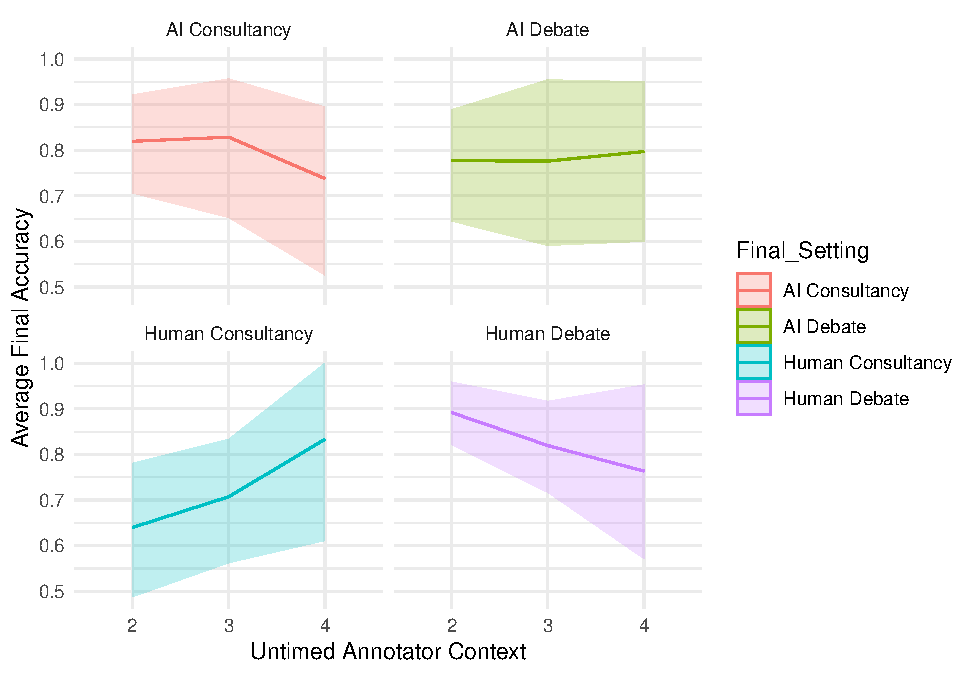
\includegraphics[width=1\linewidth]{debate-2309_files/figure-latex/Accuracy by Context Graph-3}

\subsection{Judge Skill}\label{judge-skill}

\subsubsection{Judge ``Experience''}\label{judge-experience}

\begin{Shaded}
\begin{Highlighting}[]
\NormalTok{judgments\_online }\SpecialCharTok{\%\textgreater{}\%} 
  \FunctionTok{group\_by}\NormalTok{(Final\_Setting, Participant) }\SpecialCharTok{\%\textgreater{}\%}
  \FunctionTok{arrange}\NormalTok{(}\StringTok{\textasciigrave{}}\AttributeTok{End time}\StringTok{\textasciigrave{}}\NormalTok{) }\SpecialCharTok{\%\textgreater{}\%}
  \FunctionTok{mutate}\NormalTok{(}\AttributeTok{count=}\FunctionTok{row\_number}\NormalTok{()) }\SpecialCharTok{\%\textgreater{}\%} 
  \FunctionTok{group\_by}\NormalTok{(Final\_Setting, count) }\SpecialCharTok{\%\textgreater{}\%}
  \FunctionTok{do}\NormalTok{(\{}
\NormalTok{    boot\_result }\OtherTok{\textless{}{-}} \FunctionTok{boot}\NormalTok{(}\AttributeTok{data =}\NormalTok{ .}\SpecialCharTok{$}\NormalTok{Final\_Accuracy, }\AttributeTok{statistic =}\NormalTok{ bootstrap\_mean, }\AttributeTok{R =} \DecValTok{1000}\NormalTok{)}
    \FunctionTok{data.frame}\NormalTok{(}
      \AttributeTok{mean\_accuracy =} \FunctionTok{mean}\NormalTok{(boot\_result}\SpecialCharTok{$}\NormalTok{t, }\AttributeTok{na.rm =} \ConstantTok{TRUE}\NormalTok{),}
      \AttributeTok{lower\_ci =} \FunctionTok{quantile}\NormalTok{(boot\_result}\SpecialCharTok{$}\NormalTok{t, }\FloatTok{0.025}\NormalTok{, }\AttributeTok{na.rm =} \ConstantTok{TRUE}\NormalTok{),}
      \AttributeTok{upper\_ci =} \FunctionTok{quantile}\NormalTok{(boot\_result}\SpecialCharTok{$}\NormalTok{t, }\FloatTok{0.975}\NormalTok{, }\AttributeTok{na.rm =} \ConstantTok{TRUE}\NormalTok{)}
\NormalTok{    )}
\NormalTok{  \}) }\SpecialCharTok{\%\textgreater{}\%}
  \FunctionTok{ggplot}\NormalTok{(}\FunctionTok{aes}\NormalTok{(}\AttributeTok{x =}\NormalTok{ count, }\AttributeTok{y =}\NormalTok{ mean\_accuracy, }\AttributeTok{color =}\NormalTok{ Final\_Setting, }\AttributeTok{group =}\NormalTok{ Final\_Setting)) }\SpecialCharTok{+}
  \FunctionTok{geom\_line}\NormalTok{() }\SpecialCharTok{+}
  \FunctionTok{geom\_ribbon}\NormalTok{(}\FunctionTok{aes}\NormalTok{(}\AttributeTok{ymin =}\NormalTok{ lower\_ci, }\AttributeTok{ymax =}\NormalTok{ upper\_ci, }\AttributeTok{fill =}\NormalTok{ Final\_Setting, }\AttributeTok{color =} \ConstantTok{NULL}\NormalTok{), }\AttributeTok{alpha =} \FloatTok{0.25}\NormalTok{) }\SpecialCharTok{+}
  \FunctionTok{labs}\NormalTok{(}\AttributeTok{y =} \StringTok{"Average Final Accuracy"}\NormalTok{, }\AttributeTok{x =} \StringTok{"Judging Counts"}\NormalTok{) }\SpecialCharTok{+}
  \FunctionTok{theme\_minimal}\NormalTok{() }\SpecialCharTok{+}
  \FunctionTok{facet\_wrap}\NormalTok{(}\SpecialCharTok{\textasciitilde{}}\NormalTok{ Final\_Setting)}
\end{Highlighting}
\end{Shaded}

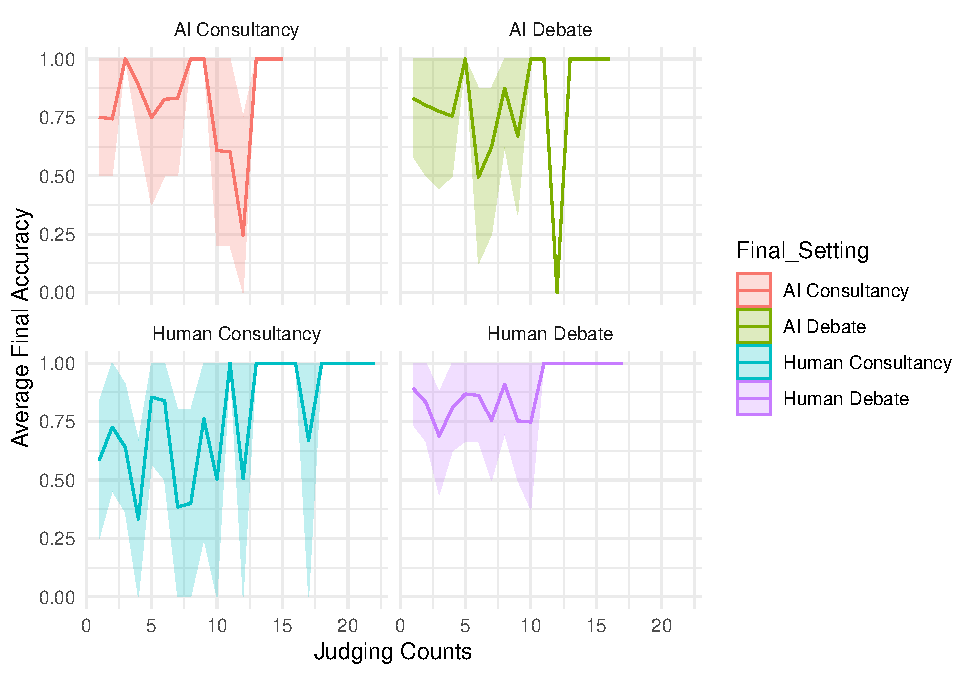
\includegraphics[width=1\linewidth]{debate-2309_files/figure-latex/unnamed-chunk-2-1}

\begin{Shaded}
\begin{Highlighting}[]
\FunctionTok{subset}\NormalTok{(judgments\_online, judgments\_online[}\StringTok{\textquotesingle{}Setting\textquotesingle{}}\NormalTok{] }\SpecialCharTok{==} \StringTok{\textquotesingle{}Human Debate\textquotesingle{}}\NormalTok{) }\SpecialCharTok{\%\textgreater{}\%} 
  \FunctionTok{group\_by}\NormalTok{(}\StringTok{\textasciigrave{}}\AttributeTok{Untimed annotator context bins}\StringTok{\textasciigrave{}}\NormalTok{, Participant) }\SpecialCharTok{\%\textgreater{}\%}
  \FunctionTok{arrange}\NormalTok{(}\StringTok{\textasciigrave{}}\AttributeTok{End time}\StringTok{\textasciigrave{}}\NormalTok{) }\SpecialCharTok{\%\textgreater{}\%}
  \FunctionTok{mutate}\NormalTok{(}\AttributeTok{count=}\FunctionTok{row\_number}\NormalTok{()) }\SpecialCharTok{\%\textgreater{}\%} 
  \FunctionTok{group\_by}\NormalTok{(}\StringTok{\textasciigrave{}}\AttributeTok{Untimed annotator context bins}\StringTok{\textasciigrave{}}\NormalTok{, count) }\SpecialCharTok{\%\textgreater{}\%}
  \FunctionTok{do}\NormalTok{(\{}
\NormalTok{    boot\_result }\OtherTok{\textless{}{-}} \FunctionTok{boot}\NormalTok{(}\AttributeTok{data =}\NormalTok{ .}\SpecialCharTok{$}\NormalTok{Final\_Accuracy, }\AttributeTok{statistic =}\NormalTok{ bootstrap\_mean, }\AttributeTok{R =} \DecValTok{1000}\NormalTok{)}
    \FunctionTok{data.frame}\NormalTok{(}
      \AttributeTok{mean\_accuracy =} \FunctionTok{mean}\NormalTok{(boot\_result}\SpecialCharTok{$}\NormalTok{t, }\AttributeTok{na.rm =} \ConstantTok{TRUE}\NormalTok{),}
      \AttributeTok{lower\_ci =} \FunctionTok{quantile}\NormalTok{(boot\_result}\SpecialCharTok{$}\NormalTok{t, }\FloatTok{0.025}\NormalTok{, }\AttributeTok{na.rm =} \ConstantTok{TRUE}\NormalTok{),}
      \AttributeTok{upper\_ci =} \FunctionTok{quantile}\NormalTok{(boot\_result}\SpecialCharTok{$}\NormalTok{t, }\FloatTok{0.975}\NormalTok{, }\AttributeTok{na.rm =} \ConstantTok{TRUE}\NormalTok{)}
\NormalTok{    )}
\NormalTok{  \}) }\SpecialCharTok{\%\textgreater{}\%}
  \FunctionTok{ggplot}\NormalTok{(}\FunctionTok{aes}\NormalTok{(}\AttributeTok{x =}\NormalTok{ count, }\AttributeTok{y =}\NormalTok{ mean\_accuracy, }\AttributeTok{color =} \StringTok{\textasciigrave{}}\AttributeTok{Untimed annotator context bins}\StringTok{\textasciigrave{}}\NormalTok{, }\AttributeTok{group =} \StringTok{\textasciigrave{}}\AttributeTok{Untimed annotator context bins}\StringTok{\textasciigrave{}}\NormalTok{)) }\SpecialCharTok{+}
  \FunctionTok{geom\_line}\NormalTok{() }\SpecialCharTok{+}
  \FunctionTok{geom\_ribbon}\NormalTok{(}\FunctionTok{aes}\NormalTok{(}\AttributeTok{ymin =}\NormalTok{ lower\_ci, }\AttributeTok{ymax =}\NormalTok{ upper\_ci, }\AttributeTok{fill =} \StringTok{\textasciigrave{}}\AttributeTok{Untimed annotator context bins}\StringTok{\textasciigrave{}}\NormalTok{, }\AttributeTok{color =} \ConstantTok{NULL}\NormalTok{), }\AttributeTok{alpha =} \FloatTok{0.25}\NormalTok{) }\SpecialCharTok{+}
  \FunctionTok{labs}\NormalTok{(}\AttributeTok{y =} \StringTok{"Average Final Accuracy"}\NormalTok{, }\AttributeTok{x =} \StringTok{"Judging Counts"}\NormalTok{) }\SpecialCharTok{+}
  \FunctionTok{theme\_minimal}\NormalTok{() }\SpecialCharTok{+}
  \FunctionTok{facet\_wrap}\NormalTok{(}\SpecialCharTok{\textasciitilde{}} \StringTok{\textasciigrave{}}\AttributeTok{Untimed annotator context bins}\StringTok{\textasciigrave{}}\NormalTok{)}
\end{Highlighting}
\end{Shaded}

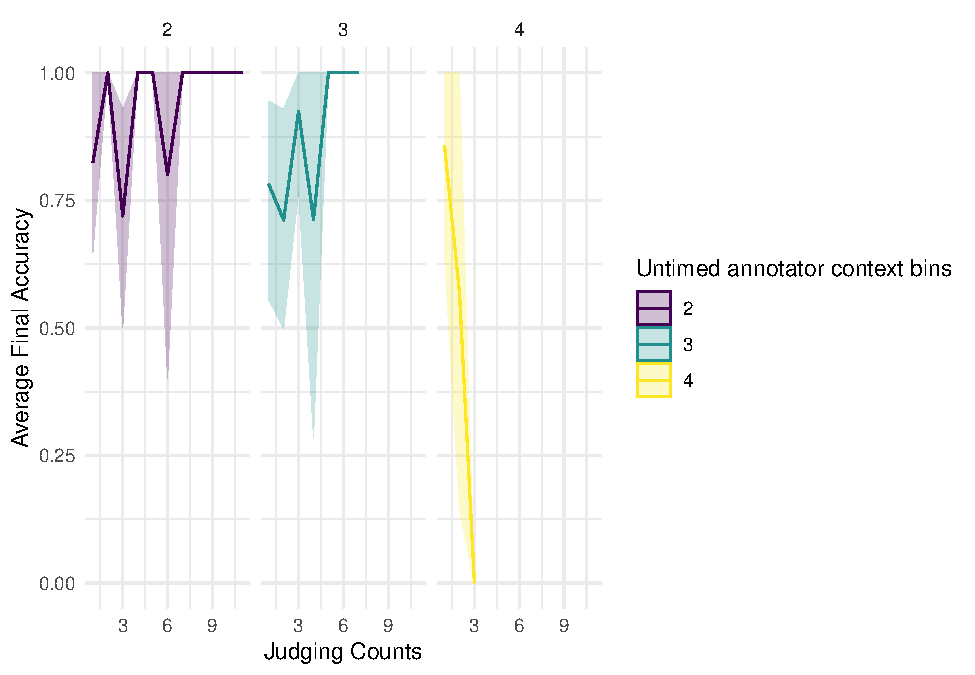
\includegraphics[width=1\linewidth]{debate-2309_files/figure-latex/unnamed-chunk-2-2}

\subsubsection{Calibration}\label{calibration}

S: (1) debaters didnt learn calibration -\textgreater{} calibration over
time? S: (2) dishonest debater tricks

\begin{Shaded}
\begin{Highlighting}[]
\FunctionTok{library}\NormalTok{(ggplot2)}
\FunctionTok{library}\NormalTok{(dplyr)}

\NormalTok{correctColor }\OtherTok{=} \StringTok{"\#008000"}
\NormalTok{incorrectColor }\OtherTok{=} \StringTok{"\#DC143C"}

\CommentTok{\# Segregate confidently correct and confidently wrong}
\NormalTok{judgments\_online}\SpecialCharTok{$}\NormalTok{confidence\_label }\OtherTok{\textless{}{-}} \FunctionTok{case\_when}\NormalTok{(}
\NormalTok{  judgments\_online}\SpecialCharTok{$}\StringTok{\textasciigrave{}}\AttributeTok{Final probability correct}\StringTok{\textasciigrave{}} \SpecialCharTok{\textgreater{}} \FloatTok{0.95} \SpecialCharTok{\textasciitilde{}} \StringTok{"Confidently Correct"}\NormalTok{,}
\NormalTok{  judgments\_online}\SpecialCharTok{$}\StringTok{\textasciigrave{}}\AttributeTok{Final probability correct}\StringTok{\textasciigrave{}} \SpecialCharTok{\textless{}} \FloatTok{0.05} \SpecialCharTok{\textasciitilde{}} \StringTok{"Confidently Wrong"}\NormalTok{,}
  \ConstantTok{TRUE} \SpecialCharTok{\textasciitilde{}} \StringTok{"Neutral"}
\NormalTok{)}

\CommentTok{\# Filter out only the rows with confidently correct and confidently wrong labels}
\NormalTok{filtered\_data }\OtherTok{\textless{}{-}}\NormalTok{ judgments\_online }\SpecialCharTok{\%\textgreater{}\%}
  \FunctionTok{filter}\NormalTok{(confidence\_label }\SpecialCharTok{!=} \StringTok{"Neutral"}\NormalTok{)}

\CommentTok{\# Count the occurrences for each setting and confidence label}
\NormalTok{count\_data }\OtherTok{\textless{}{-}}\NormalTok{ filtered\_data }\SpecialCharTok{\%\textgreater{}\%}
  \FunctionTok{group\_by}\NormalTok{(}\StringTok{\textasciigrave{}}\AttributeTok{Final\_Setting}\StringTok{\textasciigrave{}}\NormalTok{, confidence\_label) }\SpecialCharTok{\%\textgreater{}\%}
  \FunctionTok{summarise}\NormalTok{(}\AttributeTok{count =} \FunctionTok{n}\NormalTok{())}
\end{Highlighting}
\end{Shaded}

\begin{verbatim}
## `summarise()` has grouped output by 'Final_Setting'. You can override using the
## `.groups` argument.
\end{verbatim}

\begin{Shaded}
\begin{Highlighting}[]
\CommentTok{\# Plot}
\FunctionTok{ggplot}\NormalTok{(count\_data, }\FunctionTok{aes}\NormalTok{(}\AttributeTok{x =} \StringTok{\textasciigrave{}}\AttributeTok{Final\_Setting}\StringTok{\textasciigrave{}}\NormalTok{, }\AttributeTok{y =}\NormalTok{ count, }\AttributeTok{fill =}\NormalTok{ confidence\_label)) }\SpecialCharTok{+}
  \FunctionTok{geom\_bar}\NormalTok{(}\AttributeTok{stat =} \StringTok{"identity"}\NormalTok{, }\AttributeTok{position =} \StringTok{"dodge"}\NormalTok{) }\SpecialCharTok{+}
  \FunctionTok{scale\_fill\_manual}\NormalTok{(}\AttributeTok{values =} \FunctionTok{c}\NormalTok{(}\StringTok{"Confidently Correct"} \OtherTok{=}\NormalTok{ correctColor, }\StringTok{"Confidently Wrong"} \OtherTok{=}\NormalTok{ incorrectColor)) }\SpecialCharTok{+}
  \FunctionTok{labs}\NormalTok{(}\AttributeTok{title =} \StringTok{"Confident Mistakes and Correct by Setting"}\NormalTok{, }\AttributeTok{y =} \StringTok{"Count"}\NormalTok{, }\AttributeTok{x =} \StringTok{"Setting"}\NormalTok{) }\SpecialCharTok{+}
  \FunctionTok{theme\_minimal}\NormalTok{()}
\end{Highlighting}
\end{Shaded}

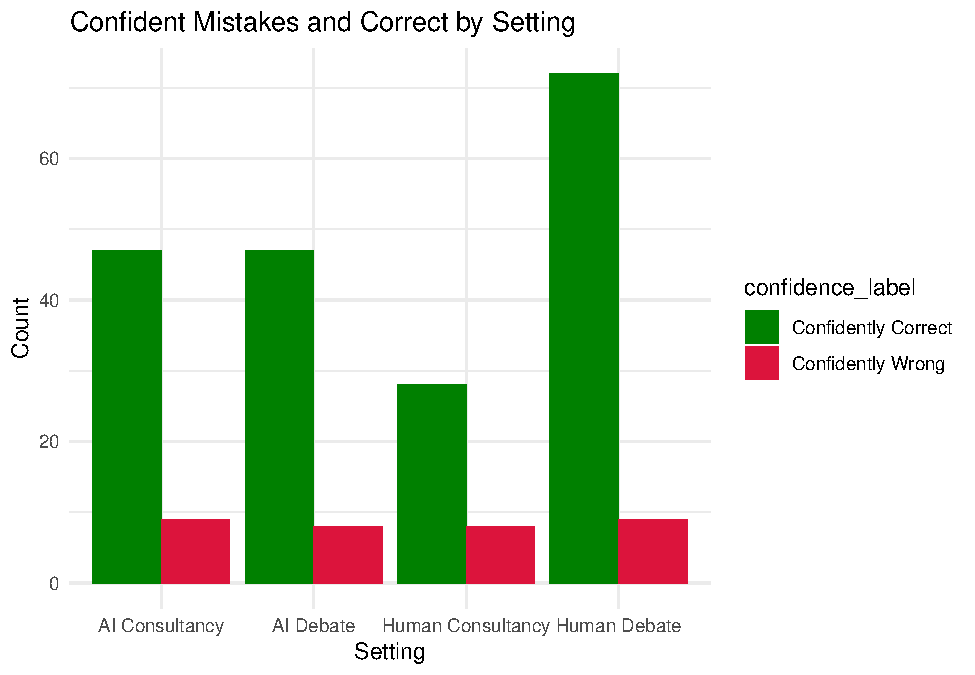
\includegraphics{debate-2309_files/figure-latex/confident mistakes-1.pdf}

\begin{Shaded}
\begin{Highlighting}[]
\CommentTok{\# Calculate the color value for each row}
\NormalTok{judgments\_online}\SpecialCharTok{$}\NormalTok{color\_value }\OtherTok{\textless{}{-}} \FunctionTok{log2}\NormalTok{(judgments\_online}\SpecialCharTok{$}\StringTok{\textasciigrave{}}\AttributeTok{Final probability correct}\StringTok{\textasciigrave{}}\NormalTok{) }\SpecialCharTok{{-}}\NormalTok{ (}\FloatTok{0.05} \SpecialCharTok{*}\NormalTok{ judgments\_online}\SpecialCharTok{$}\StringTok{\textasciigrave{}}\AttributeTok{Number of judge continues}\StringTok{\textasciigrave{}}\NormalTok{)}

\CommentTok{\# Count the occurrences for each setting and \textquotesingle{}Final probability correct\textquotesingle{} value}
\NormalTok{count\_data }\OtherTok{\textless{}{-}}\NormalTok{ judgments\_online }\SpecialCharTok{\%\textgreater{}\%}
  \FunctionTok{group\_by}\NormalTok{(}\StringTok{\textasciigrave{}}\AttributeTok{Final\_Setting}\StringTok{\textasciigrave{}}\NormalTok{, }\StringTok{\textasciigrave{}}\AttributeTok{Final probability correct}\StringTok{\textasciigrave{}}\NormalTok{, color\_value) }\SpecialCharTok{\%\textgreater{}\%}
  \FunctionTok{summarise}\NormalTok{(}\AttributeTok{count =} \FunctionTok{n}\NormalTok{())}
\end{Highlighting}
\end{Shaded}

\begin{verbatim}
## `summarise()` has grouped output by 'Final_Setting', 'Final probability
## correct'. You can override using the `.groups` argument.
\end{verbatim}

\begin{Shaded}
\begin{Highlighting}[]
\CommentTok{\# Plot}
\FunctionTok{ggplot}\NormalTok{(count\_data, }\FunctionTok{aes}\NormalTok{(}\AttributeTok{x =} \StringTok{\textasciigrave{}}\AttributeTok{Final\_Setting}\StringTok{\textasciigrave{}}\NormalTok{, }\AttributeTok{y =}\NormalTok{ count, }\AttributeTok{fill =}\NormalTok{ color\_value, }\AttributeTok{group =} \StringTok{\textasciigrave{}}\AttributeTok{Final probability correct}\StringTok{\textasciigrave{}}\NormalTok{)) }\SpecialCharTok{+}
  \FunctionTok{geom\_bar}\NormalTok{(}\AttributeTok{stat =} \StringTok{"identity"}\NormalTok{, }\AttributeTok{position =} \StringTok{"stack"}\NormalTok{) }\SpecialCharTok{+}
  \FunctionTok{scale\_fill\_gradient}\NormalTok{(}\AttributeTok{low =} \StringTok{"\#DC143C"}\NormalTok{, }\AttributeTok{high =} \StringTok{"\#008000"}\NormalTok{) }\SpecialCharTok{+}  \CommentTok{\# Adjust as needed}
  \FunctionTok{labs}\NormalTok{(}\AttributeTok{title =} \StringTok{"Distribution of Final Probabilities by Setting"}\NormalTok{, }\AttributeTok{y =} \StringTok{"Count"}\NormalTok{, }\AttributeTok{x =} \StringTok{"Setting"}\NormalTok{) }\SpecialCharTok{+}
  \FunctionTok{theme\_minimal}\NormalTok{()}
\end{Highlighting}
\end{Shaded}

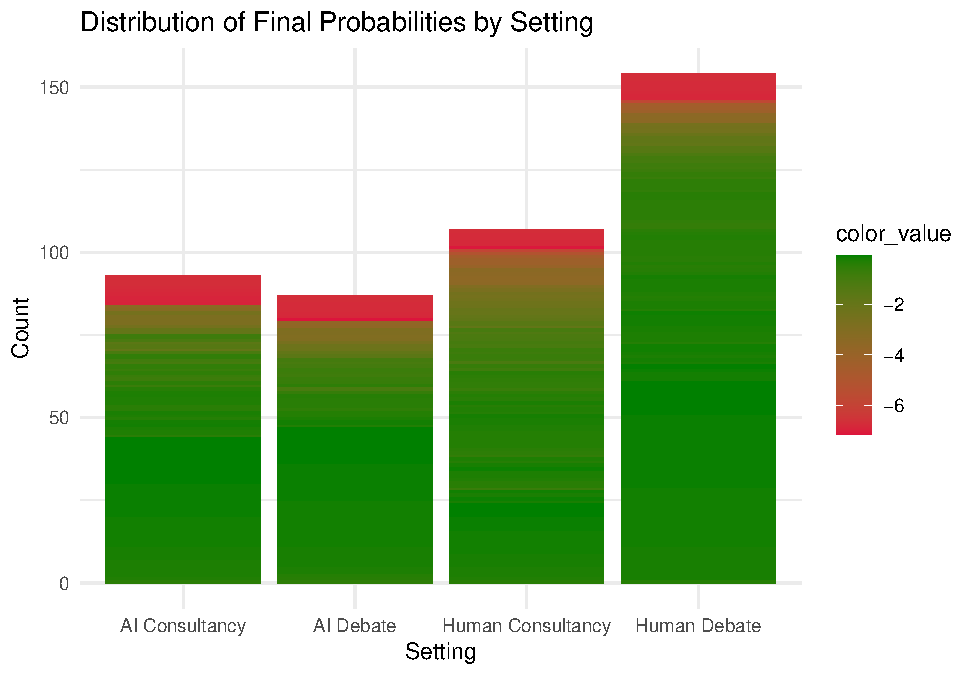
\includegraphics{debate-2309_files/figure-latex/confident mistakes-2.pdf}

\begin{Shaded}
\begin{Highlighting}[]
\ImportTok{import}\NormalTok{ pandas }\ImportTok{as}\NormalTok{ pd}
\ImportTok{import}\NormalTok{ numpy }\ImportTok{as}\NormalTok{ np}
\ImportTok{import}\NormalTok{ matplotlib.pyplot }\ImportTok{as}\NormalTok{ plt}
\ImportTok{from}\NormalTok{ sklearn.calibration }\ImportTok{import}\NormalTok{ calibration\_curve}

\KeywordTok{def}\NormalTok{ calibration\_plot(df, setting\_name, ax}\OperatorTok{=}\VariableTok{None}\NormalTok{):}
\NormalTok{    df[}\StringTok{\textquotesingle{}outcome\textquotesingle{}}\NormalTok{] }\OperatorTok{=}\NormalTok{ pd.Series(df[}\StringTok{\textquotesingle{}Final probability correct\textquotesingle{}}\NormalTok{] }\OperatorTok{\textgreater{}} \FloatTok{0.5}\NormalTok{, dtype}\OperatorTok{=}\BuiltInTok{int}\NormalTok{)}
\NormalTok{    df[}\StringTok{\textquotesingle{}confidence\textquotesingle{}}\NormalTok{] }\OperatorTok{=}\NormalTok{ df[}\StringTok{\textquotesingle{}Final probability correct\textquotesingle{}}\NormalTok{].}\BuiltInTok{apply}\NormalTok{(}\KeywordTok{lambda}\NormalTok{ x: x }\ControlFlowTok{if}\NormalTok{ x }\OperatorTok{\textgreater{}} \FloatTok{0.5} \ControlFlowTok{else} \DecValTok{1} \OperatorTok{{-}}\NormalTok{ x)}
\NormalTok{    df[}\StringTok{\textquotesingle{}bins\textquotesingle{}}\NormalTok{] }\OperatorTok{=}\NormalTok{ pd.cut(df[}\StringTok{\textquotesingle{}confidence\textquotesingle{}}\NormalTok{], [}\FloatTok{0.5}\NormalTok{, }\FloatTok{0.6}\NormalTok{, }\FloatTok{0.7}\NormalTok{, }\FloatTok{0.8}\NormalTok{, }\FloatTok{0.9}\NormalTok{, }\FloatTok{0.95}\NormalTok{, }\FloatTok{0.99}\NormalTok{])}
    \CommentTok{\# Group by bins and calculate the mean outcome}
\NormalTok{    df\_grouped }\OperatorTok{=}\NormalTok{ df.groupby(}\StringTok{\textquotesingle{}bins\textquotesingle{}}\NormalTok{)[}\StringTok{\textquotesingle{}outcome\textquotesingle{}}\NormalTok{].mean().reset\_index()}
    \CommentTok{\# Compute standard error in each bin}
\NormalTok{    std\_error }\OperatorTok{=}\NormalTok{ df.groupby(}\StringTok{\textquotesingle{}bins\textquotesingle{}}\NormalTok{)[}\StringTok{\textquotesingle{}outcome\textquotesingle{}}\NormalTok{].}\BuiltInTok{apply}\NormalTok{(}\KeywordTok{lambda}\NormalTok{ x: x.std() }\OperatorTok{/}\NormalTok{ np.sqrt(}\BuiltInTok{len}\NormalTok{(x)) }\ControlFlowTok{if} \BuiltInTok{len}\NormalTok{(x) }\OperatorTok{\textgreater{}} \DecValTok{1} \ControlFlowTok{else} \DecValTok{0}\NormalTok{)}
\NormalTok{    df\_grouped[}\StringTok{\textquotesingle{}std\_error\textquotesingle{}}\NormalTok{] }\OperatorTok{=}\NormalTok{ df[}\StringTok{\textquotesingle{}bins\textquotesingle{}}\NormalTok{].cat.categories.}\BuiltInTok{map}\NormalTok{(std\_error)}
    \ControlFlowTok{if}\NormalTok{ ax }\KeywordTok{is} \VariableTok{None}\NormalTok{:}
\NormalTok{        plt.rcParams.update(\{}\StringTok{\textquotesingle{}font.size\textquotesingle{}}\NormalTok{: }\DecValTok{16}\NormalTok{\})}
\NormalTok{        fig, ax }\OperatorTok{=}\NormalTok{ plt.subplots(figsize}\OperatorTok{=}\NormalTok{(}\DecValTok{8}\NormalTok{, }\DecValTok{6}\NormalTok{))}
    \CommentTok{\# Plot the calibration curve with error bars}
\NormalTok{    ax.plot(df\_grouped[}\StringTok{\textquotesingle{}bins\textquotesingle{}}\NormalTok{].}\BuiltInTok{apply}\NormalTok{(}\KeywordTok{lambda}\NormalTok{ x: x.mid), df\_grouped[}\StringTok{\textquotesingle{}outcome\textquotesingle{}}\NormalTok{], marker}\OperatorTok{=}\StringTok{\textquotesingle{}o\textquotesingle{}}\NormalTok{, linewidth}\OperatorTok{=}\DecValTok{2}\NormalTok{, label}\OperatorTok{=}\StringTok{\textquotesingle{}Calibration Curve\textquotesingle{}}\NormalTok{)}
\NormalTok{    ax.errorbar(df\_grouped[}\StringTok{\textquotesingle{}bins\textquotesingle{}}\NormalTok{].}\BuiltInTok{apply}\NormalTok{(}\KeywordTok{lambda}\NormalTok{ x: x.mid), df\_grouped[}\StringTok{\textquotesingle{}outcome\textquotesingle{}}\NormalTok{], yerr}\OperatorTok{=}\NormalTok{df\_grouped[}\StringTok{\textquotesingle{}std\_error\textquotesingle{}}\NormalTok{], fmt}\OperatorTok{=}\StringTok{\textquotesingle{}o\textquotesingle{}}\NormalTok{, capsize}\OperatorTok{=}\DecValTok{5}\NormalTok{, linewidth}\OperatorTok{=}\DecValTok{2}\NormalTok{, label}\OperatorTok{=}\StringTok{\textquotesingle{}Error Bars\textquotesingle{}}\NormalTok{)}
\NormalTok{    ax.set\_xlabel(}\StringTok{\textquotesingle{}Final judge probability\textquotesingle{}}\NormalTok{)}
\NormalTok{    ax.set\_ylabel(}\StringTok{\textquotesingle{}Accuracy\textquotesingle{}}\NormalTok{)}
\NormalTok{    ax.set\_title(}\SpecialStringTok{f\textquotesingle{}Judge calibration for }\SpecialCharTok{\{}\NormalTok{setting\_name}\SpecialCharTok{\}}\SpecialStringTok{\textquotesingle{}}\NormalTok{)}
\NormalTok{    ax.plot([}\FloatTok{0.5}\NormalTok{, }\DecValTok{1}\NormalTok{], [}\FloatTok{0.5}\NormalTok{, }\DecValTok{1}\NormalTok{], linestyle}\OperatorTok{=}\StringTok{\textquotesingle{}{-}{-}\textquotesingle{}}\NormalTok{, color}\OperatorTok{=}\StringTok{\textquotesingle{}gray\textquotesingle{}}\NormalTok{, label}\OperatorTok{=}\StringTok{\textquotesingle{}Perfect Calibration\textquotesingle{}}\NormalTok{)}
\NormalTok{    ax.grid(}\VariableTok{True}\NormalTok{)}
\NormalTok{    ax.legend()}
    \CommentTok{\# Calculate ECE}
\NormalTok{    actual\_labels }\OperatorTok{=}\NormalTok{ df[}\StringTok{\textquotesingle{}outcome\textquotesingle{}}\NormalTok{].values}
\NormalTok{    predicted\_probs }\OperatorTok{=}\NormalTok{ df[}\StringTok{\textquotesingle{}Final probability correct\textquotesingle{}}\NormalTok{].values}
\NormalTok{    prob\_true, prob\_pred }\OperatorTok{=}\NormalTok{ calibration\_curve(actual\_labels, predicted\_probs, n\_bins}\OperatorTok{=}\DecValTok{10}\NormalTok{)}
\NormalTok{    ece }\OperatorTok{=}\NormalTok{ np.mean(np.}\BuiltInTok{abs}\NormalTok{(prob\_pred }\OperatorTok{{-}}\NormalTok{ prob\_true) }\OperatorTok{*}\NormalTok{ (prob\_true.size }\OperatorTok{/} \BuiltInTok{len}\NormalTok{(actual\_labels)))}
    \CommentTok{\# Print ECE}
    \BuiltInTok{print}\NormalTok{(}\SpecialStringTok{f"Expected Calibration Error (ECE) for }\SpecialCharTok{\{}\NormalTok{setting\_name}\SpecialCharTok{\}}\SpecialStringTok{: }\SpecialCharTok{\{}\NormalTok{ece}\SpecialCharTok{:.4f\}}\SpecialStringTok{"}\NormalTok{)}
\NormalTok{    plt.show()}
\NormalTok{    plt.rcParams.update(\{}\StringTok{\textquotesingle{}font.size\textquotesingle{}}\NormalTok{: plt.rcParamsDefault[}\StringTok{\textquotesingle{}font.size\textquotesingle{}}\NormalTok{]\})}

\CommentTok{\# Loop through each unique setting and create a calibration plot}
\ControlFlowTok{for}\NormalTok{ setting }\KeywordTok{in}\NormalTok{ judgments\_online[}\StringTok{\textquotesingle{}Final\_Setting\textquotesingle{}}\NormalTok{].unique():}
\NormalTok{    setting\_df }\OperatorTok{=}\NormalTok{ judgments\_online[judgments[}\StringTok{\textquotesingle{}Final\_Setting\textquotesingle{}}\NormalTok{] }\OperatorTok{==}\NormalTok{ setting].copy()}
\NormalTok{    calibration\_plot(setting\_df, setting)}
\end{Highlighting}
\end{Shaded}

\begin{verbatim}
## Expected Calibration Error (ECE) for AI Consultancy: 0.0213
## Expected Calibration Error (ECE) for Human Debate: 0.0152
## Expected Calibration Error (ECE) for AI Debate: 0.0268
## Expected Calibration Error (ECE) for Human Consultancy: 0.0220
## 
## <string>:4: UserWarning: Boolean Series key will be reindexed to match DataFrame index.
## <string>:7: FutureWarning: The default of observed=False is deprecated and will be changed to True in a future version of pandas. Pass observed=False to retain current behavior or observed=True to adopt the future default and silence this warning.
## <string>:9: FutureWarning: The default of observed=False is deprecated and will be changed to True in a future version of pandas. Pass observed=False to retain current behavior or observed=True to adopt the future default and silence this warning.
## <string>:4: UserWarning: Boolean Series key will be reindexed to match DataFrame index.
## <string>:7: FutureWarning: The default of observed=False is deprecated and will be changed to True in a future version of pandas. Pass observed=False to retain current behavior or observed=True to adopt the future default and silence this warning.
## <string>:9: FutureWarning: The default of observed=False is deprecated and will be changed to True in a future version of pandas. Pass observed=False to retain current behavior or observed=True to adopt the future default and silence this warning.
## <string>:4: UserWarning: Boolean Series key will be reindexed to match DataFrame index.
## <string>:7: FutureWarning: The default of observed=False is deprecated and will be changed to True in a future version of pandas. Pass observed=False to retain current behavior or observed=True to adopt the future default and silence this warning.
## <string>:9: FutureWarning: The default of observed=False is deprecated and will be changed to True in a future version of pandas. Pass observed=False to retain current behavior or observed=True to adopt the future default and silence this warning.
## <string>:4: UserWarning: Boolean Series key will be reindexed to match DataFrame index.
## <string>:7: FutureWarning: The default of observed=False is deprecated and will be changed to True in a future version of pandas. Pass observed=False to retain current behavior or observed=True to adopt the future default and silence this warning.
## <string>:9: FutureWarning: The default of observed=False is deprecated and will be changed to True in a future version of pandas. Pass observed=False to retain current behavior or observed=True to adopt the future default and silence this warning.
\end{verbatim}

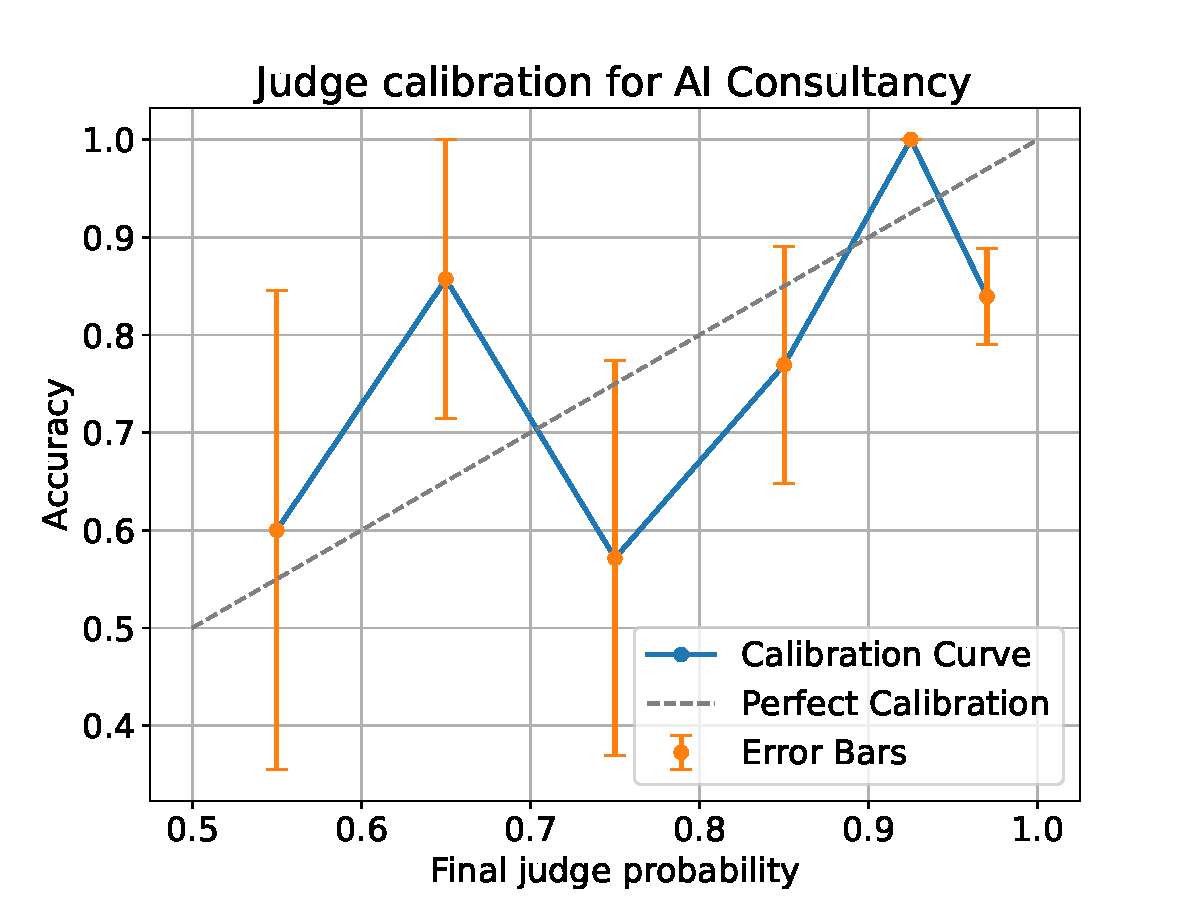
\includegraphics[width=1\linewidth]{debate-2309_files/figure-latex/calibration-1}
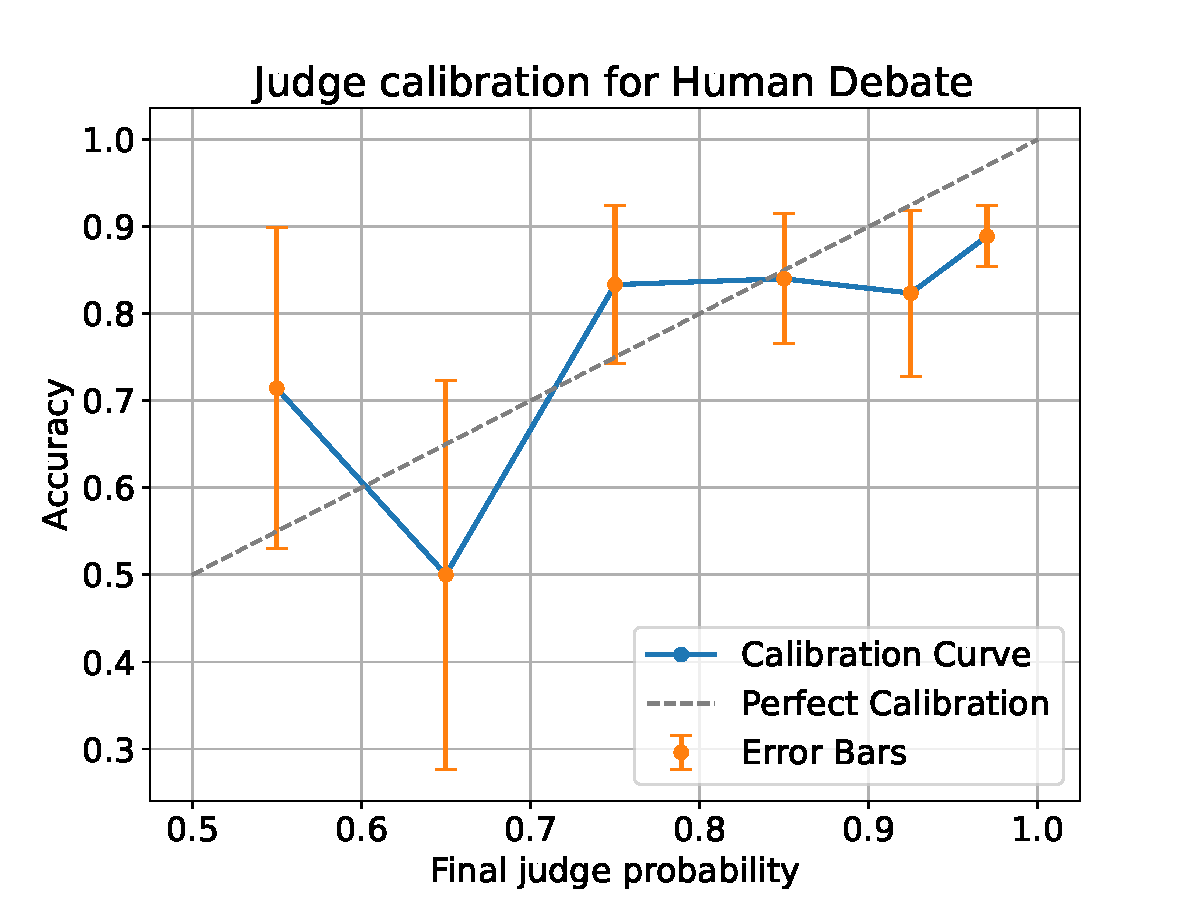
\includegraphics[width=1\linewidth]{debate-2309_files/figure-latex/calibration-2}
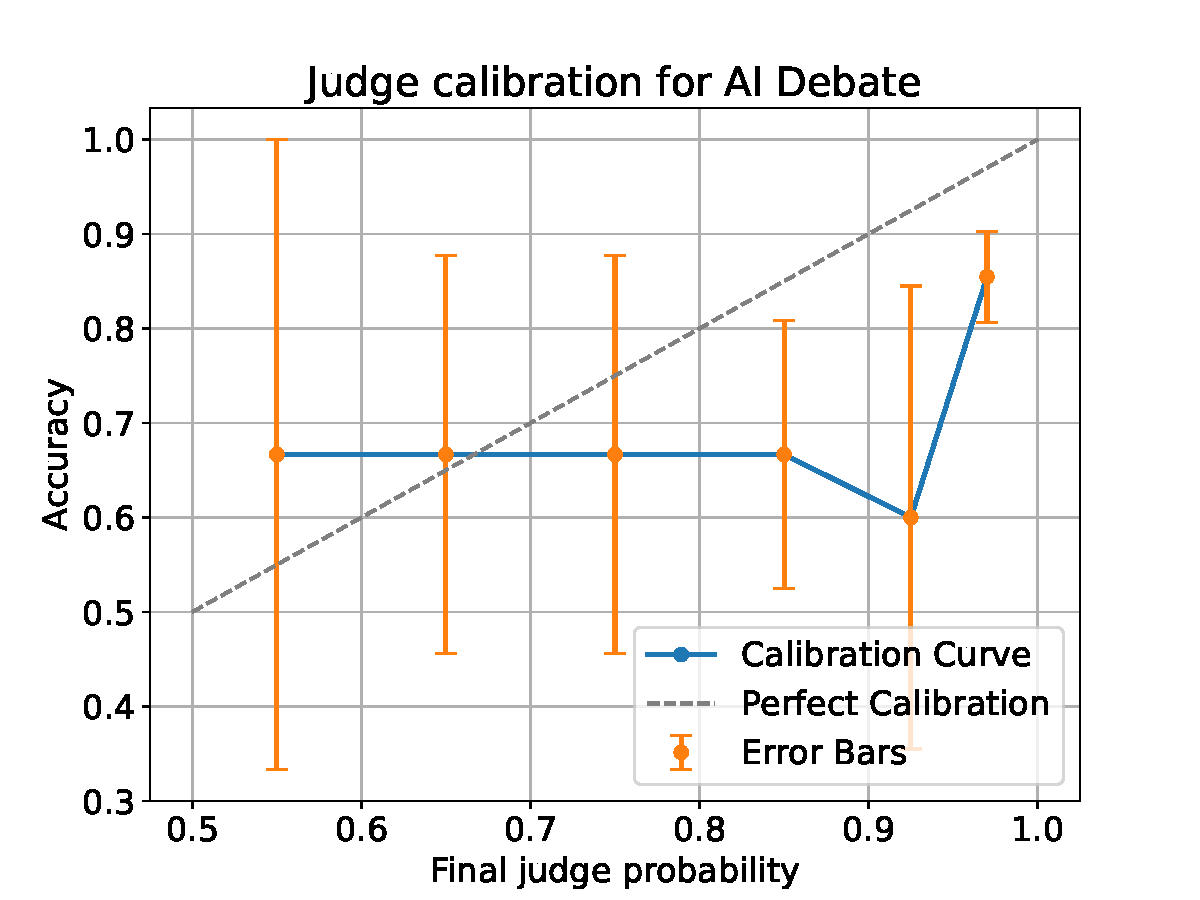
\includegraphics[width=1\linewidth]{debate-2309_files/figure-latex/calibration-3}
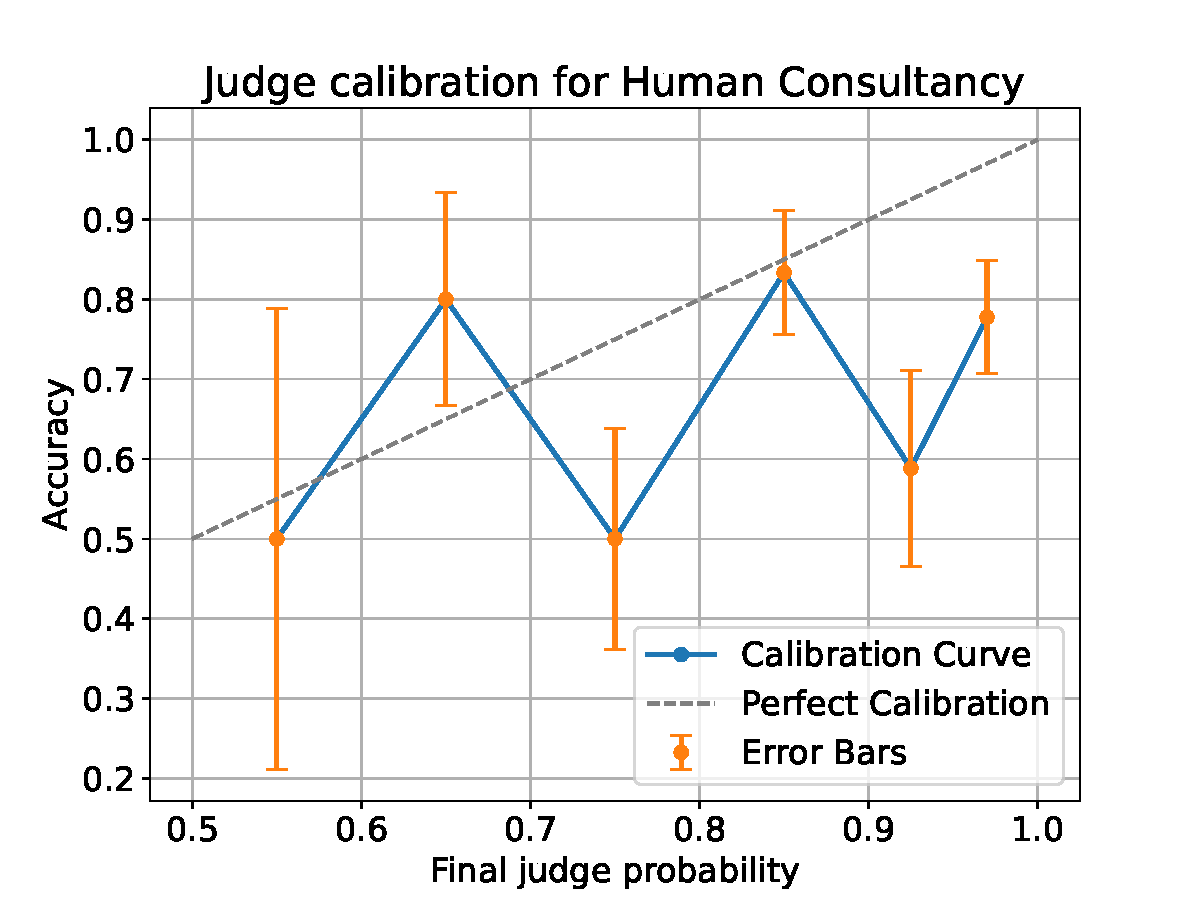
\includegraphics[width=1\linewidth]{debate-2309_files/figure-latex/calibration-4}

\subsubsection{Judge Involvement}\label{judge-involvement}

\subsubsection{Judge Mistakes}\label{judge-mistakes}

\subsection{Debater Skill}\label{debater-skill}

\begin{Shaded}
\begin{Highlighting}[]
\NormalTok{random.intercept.model }\OtherTok{=} \FunctionTok{lmer}\NormalTok{(}\StringTok{\textasciigrave{}}\AttributeTok{Final probability correct}\StringTok{\textasciigrave{}} \SpecialCharTok{\textasciitilde{}}\NormalTok{  (}\DecValTok{1}\SpecialCharTok{|}\NormalTok{Final\_Setting), }
                              \AttributeTok{data =}\NormalTok{ judgments, }\AttributeTok{REML =} \ConstantTok{TRUE}\NormalTok{)}

\NormalTok{judgments}\SpecialCharTok{$}\NormalTok{random.intercept.preds }\OtherTok{=} \FunctionTok{predict}\NormalTok{(random.intercept.model)}

\FunctionTok{colnames}\NormalTok{(judgments)}
\end{Highlighting}
\end{Shaded}

\begin{verbatim}
##  [1] "Participant"                            
##  [2] "base_room_name"                         
##  [3] "Room name"                              
##  [4] "Room start time"                        
##  [5] "Role"                                   
##  [6] "Is turn"                                
##  [7] "Is over"                                
##  [8] "Number of judge continues"              
##  [9] "Final probability correct"              
## [10] "Offline judging start time"             
## [11] "Offline judging end time"               
## [12] "other"                                  
## [13] "factual informativeness (comparative).1"
## [14] "factual informativeness (comparative).2"
## [15] "facts versus semantics (single)"        
## [16] "factual accuracy (single)"              
## [17] "clarity.1"                              
## [18] "clarity.2"                              
## [19] "factual accuracy.1"                     
## [20] "factual accuracy.2"                     
## [21] "judge reasoning"                        
## [22] "reason for outcome"                     
## [23] "protocol"                               
## [24] "evidence use.1"                         
## [25] "evidence use.2"                         
## [26] "evidence in story.1"                    
## [27] "evidence in story.2"                    
## [28] "other factors"                          
## [29] "judge adaptation (single)"              
## [30] "evidence in debate.1"                   
## [31] "evidence in debate.2"                   
## [32] "interface"                              
## [33] "evidence in debate (single)"            
## [34] "facts versus semantics.1"               
## [35] "facts versus semantics.2"               
## [36] "clash.1"                                
## [37] "clash.2"                                
## [38] "identity guesses.Judge"                 
## [39] "identity guesses.Debater A"             
## [40] "identity guesses.Debater B"             
## [41] "judge adaptation.1"                     
## [42] "judge adaptation.2"                     
## [43] "subjective correctness"                 
## [44] "evidence use (single)"                  
## [45] "factual informativeness (total)"        
## [46] "judge strategies"                       
## [47] "clarity (single)"                       
## [48] "Debater A"                              
## [49] "Debater B"                              
## [50] "Honest debater"                         
## [51] "Dishonest debater"                      
## [52] "Is single debater"                      
## [53] "Has honest debater"                     
## [54] "Final_Setting"                          
## [55] "Setting"                                
## [56] "Question"                               
## [57] "Article ID"                             
## [58] "Speed annotator accuracy bins"          
## [59] "Untimed annotator context bins"         
## [60] "Speed annotator accuracy"               
## [61] "Untimed annotator context"              
## [62] "Is offline"                             
## [63] "End time"                               
## [64] "Last modified time"                     
## [65] "Final_Accuracy"                         
## [66] "random.intercept.preds"
\end{verbatim}

\begin{Shaded}
\begin{Highlighting}[]
\NormalTok{dishonest }\OtherTok{\textless{}{-}}\NormalTok{ judgments[}\SpecialCharTok{!}\FunctionTok{is.na}\NormalTok{(judgments}\SpecialCharTok{$}\StringTok{\textasciigrave{}}\AttributeTok{Dishonest debater}\StringTok{\textasciigrave{}}\NormalTok{), ]}
\NormalTok{model3 }\OtherTok{\textless{}{-}} \FunctionTok{glm}\NormalTok{(Final\_Accuracy }\SpecialCharTok{\textasciitilde{}} \FunctionTok{relevel}\NormalTok{(}\FunctionTok{factor}\NormalTok{(}\StringTok{\textasciigrave{}}\AttributeTok{Dishonest debater}\StringTok{\textasciigrave{}}\NormalTok{), }\StringTok{\textquotesingle{}Shlomo Kofman\textquotesingle{}}\NormalTok{) }\SpecialCharTok{+} \FunctionTok{relevel}\NormalTok{(}\FunctionTok{factor}\NormalTok{(Final\_Setting), }\StringTok{\textquotesingle{}Human Debate\textquotesingle{}}\NormalTok{), }\AttributeTok{family =} \StringTok{\textquotesingle{}binomial\textquotesingle{}}\NormalTok{, }\AttributeTok{data =}\NormalTok{ judgments[}\SpecialCharTok{!}\FunctionTok{is.na}\NormalTok{(judgments}\SpecialCharTok{$}\StringTok{\textasciigrave{}}\AttributeTok{Dishonest debater}\StringTok{\textasciigrave{}}\NormalTok{), ])}
\FunctionTok{summary}\NormalTok{(model3)}
\end{Highlighting}
\end{Shaded}

\begin{verbatim}
## 
## Call:
## glm(formula = Final_Accuracy ~ relevel(factor(`Dishonest debater`), 
##     "Shlomo Kofman") + relevel(factor(Final_Setting), "Human Debate"), 
##     family = "binomial", data = judgments[!is.na(judgments$`Dishonest debater`), 
##         ])
## 
## Coefficients: (1 not defined because of singularities)
##                                                                           Estimate
## (Intercept)                                                                0.52739
## relevel(factor(`Dishonest debater`), "Shlomo Kofman")Adelle Fernando       0.95584
## relevel(factor(`Dishonest debater`), "Shlomo Kofman")Aliyaah Toussaint     2.41514
## relevel(factor(`Dishonest debater`), "Shlomo Kofman")Anuj Jain             1.47707
## relevel(factor(`Dishonest debater`), "Shlomo Kofman")David Rein            1.41852
## relevel(factor(`Dishonest debater`), "Shlomo Kofman")Emmanuel Makinde     17.03868
## relevel(factor(`Dishonest debater`), "Shlomo Kofman")Ethan Rosen           1.45361
## relevel(factor(`Dishonest debater`), "Shlomo Kofman")GPT-4                 0.75355
## relevel(factor(`Dishonest debater`), "Shlomo Kofman")Jackson Petty         2.08187
## relevel(factor(`Dishonest debater`), "Shlomo Kofman")Jessica Li            0.53268
## relevel(factor(`Dishonest debater`), "Shlomo Kofman")Julian Michael        2.41705
## relevel(factor(`Dishonest debater`), "Shlomo Kofman")Julien Dirani         1.55205
## relevel(factor(`Dishonest debater`), "Shlomo Kofman")Max Layden           17.03868
## relevel(factor(`Dishonest debater`), "Shlomo Kofman")Noor Mirza-Rashid    -0.05738
## relevel(factor(`Dishonest debater`), "Shlomo Kofman")Reeya Kansra          1.44916
## relevel(factor(`Dishonest debater`), "Shlomo Kofman")Salsabila Mahdi       1.47874
## relevel(factor(`Dishonest debater`), "Shlomo Kofman")Sam Jin               1.30012
## relevel(factor(`Dishonest debater`), "Shlomo Kofman")Sean Wang             1.43988
## relevel(factor(`Dishonest debater`), "Shlomo Kofman")Shreeram Modi         1.45605
## relevel(factor(`Dishonest debater`), "Shlomo Kofman")Vishakh Padmakumar   17.03868
## relevel(factor(Final_Setting), "Human Debate")AI Consultancy               0.66498
## relevel(factor(Final_Setting), "Human Debate")AI Debate                         NA
## relevel(factor(Final_Setting), "Human Debate")Human Consultancy           -1.33091
##                                                                         Std. Error
## (Intercept)                                                                0.66115
## relevel(factor(`Dishonest debater`), "Shlomo Kofman")Adelle Fernando       0.73718
## relevel(factor(`Dishonest debater`), "Shlomo Kofman")Aliyaah Toussaint     1.23691
## relevel(factor(`Dishonest debater`), "Shlomo Kofman")Anuj Jain             0.84884
## relevel(factor(`Dishonest debater`), "Shlomo Kofman")David Rein            0.90447
## relevel(factor(`Dishonest debater`), "Shlomo Kofman")Emmanuel Makinde   2797.44202
## relevel(factor(`Dishonest debater`), "Shlomo Kofman")Ethan Rosen           0.84947
## relevel(factor(`Dishonest debater`), "Shlomo Kofman")GPT-4                 0.70782
## relevel(factor(`Dishonest debater`), "Shlomo Kofman")Jackson Petty         0.98698
## relevel(factor(`Dishonest debater`), "Shlomo Kofman")Jessica Li            0.74081
## relevel(factor(`Dishonest debater`), "Shlomo Kofman")Julian Michael        1.22055
## relevel(factor(`Dishonest debater`), "Shlomo Kofman")Julien Dirani         1.24985
## relevel(factor(`Dishonest debater`), "Shlomo Kofman")Max Layden         3956.18038
## relevel(factor(`Dishonest debater`), "Shlomo Kofman")Noor Mirza-Rashid     0.87300
## relevel(factor(`Dishonest debater`), "Shlomo Kofman")Reeya Kansra          0.90748
## relevel(factor(`Dishonest debater`), "Shlomo Kofman")Salsabila Mahdi       0.79085
## relevel(factor(`Dishonest debater`), "Shlomo Kofman")Sam Jin               0.93690
## relevel(factor(`Dishonest debater`), "Shlomo Kofman")Sean Wang             0.75579
## relevel(factor(`Dishonest debater`), "Shlomo Kofman")Shreeram Modi         0.75586
## relevel(factor(`Dishonest debater`), "Shlomo Kofman")Vishakh Padmakumar  863.30958
## relevel(factor(Final_Setting), "Human Debate")AI Consultancy               0.54080
## relevel(factor(Final_Setting), "Human Debate")AI Debate                         NA
## relevel(factor(Final_Setting), "Human Debate")Human Consultancy            0.32388
##                                                                         z value
## (Intercept)                                                               0.798
## relevel(factor(`Dishonest debater`), "Shlomo Kofman")Adelle Fernando      1.297
## relevel(factor(`Dishonest debater`), "Shlomo Kofman")Aliyaah Toussaint    1.953
## relevel(factor(`Dishonest debater`), "Shlomo Kofman")Anuj Jain            1.740
## relevel(factor(`Dishonest debater`), "Shlomo Kofman")David Rein           1.568
## relevel(factor(`Dishonest debater`), "Shlomo Kofman")Emmanuel Makinde     0.006
## relevel(factor(`Dishonest debater`), "Shlomo Kofman")Ethan Rosen          1.711
## relevel(factor(`Dishonest debater`), "Shlomo Kofman")GPT-4                1.065
## relevel(factor(`Dishonest debater`), "Shlomo Kofman")Jackson Petty        2.109
## relevel(factor(`Dishonest debater`), "Shlomo Kofman")Jessica Li           0.719
## relevel(factor(`Dishonest debater`), "Shlomo Kofman")Julian Michael       1.980
## relevel(factor(`Dishonest debater`), "Shlomo Kofman")Julien Dirani        1.242
## relevel(factor(`Dishonest debater`), "Shlomo Kofman")Max Layden           0.004
## relevel(factor(`Dishonest debater`), "Shlomo Kofman")Noor Mirza-Rashid   -0.066
## relevel(factor(`Dishonest debater`), "Shlomo Kofman")Reeya Kansra         1.597
## relevel(factor(`Dishonest debater`), "Shlomo Kofman")Salsabila Mahdi      1.870
## relevel(factor(`Dishonest debater`), "Shlomo Kofman")Sam Jin              1.388
## relevel(factor(`Dishonest debater`), "Shlomo Kofman")Sean Wang            1.905
## relevel(factor(`Dishonest debater`), "Shlomo Kofman")Shreeram Modi        1.926
## relevel(factor(`Dishonest debater`), "Shlomo Kofman")Vishakh Padmakumar   0.020
## relevel(factor(Final_Setting), "Human Debate")AI Consultancy              1.230
## relevel(factor(Final_Setting), "Human Debate")AI Debate                      NA
## relevel(factor(Final_Setting), "Human Debate")Human Consultancy          -4.109
##                                                                          Pr(>|z|)
## (Intercept)                                                                0.4251
## relevel(factor(`Dishonest debater`), "Shlomo Kofman")Adelle Fernando       0.1948
## relevel(factor(`Dishonest debater`), "Shlomo Kofman")Aliyaah Toussaint     0.0509
## relevel(factor(`Dishonest debater`), "Shlomo Kofman")Anuj Jain             0.0818
## relevel(factor(`Dishonest debater`), "Shlomo Kofman")David Rein            0.1168
## relevel(factor(`Dishonest debater`), "Shlomo Kofman")Emmanuel Makinde      0.9951
## relevel(factor(`Dishonest debater`), "Shlomo Kofman")Ethan Rosen           0.0870
## relevel(factor(`Dishonest debater`), "Shlomo Kofman")GPT-4                 0.2871
## relevel(factor(`Dishonest debater`), "Shlomo Kofman")Jackson Petty         0.0349
## relevel(factor(`Dishonest debater`), "Shlomo Kofman")Jessica Li            0.4721
## relevel(factor(`Dishonest debater`), "Shlomo Kofman")Julian Michael        0.0477
## relevel(factor(`Dishonest debater`), "Shlomo Kofman")Julien Dirani         0.2143
## relevel(factor(`Dishonest debater`), "Shlomo Kofman")Max Layden            0.9966
## relevel(factor(`Dishonest debater`), "Shlomo Kofman")Noor Mirza-Rashid     0.9476
## relevel(factor(`Dishonest debater`), "Shlomo Kofman")Reeya Kansra          0.1103
## relevel(factor(`Dishonest debater`), "Shlomo Kofman")Salsabila Mahdi       0.0615
## relevel(factor(`Dishonest debater`), "Shlomo Kofman")Sam Jin               0.1652
## relevel(factor(`Dishonest debater`), "Shlomo Kofman")Sean Wang             0.0568
## relevel(factor(`Dishonest debater`), "Shlomo Kofman")Shreeram Modi         0.0541
## relevel(factor(`Dishonest debater`), "Shlomo Kofman")Vishakh Padmakumar    0.9843
## relevel(factor(Final_Setting), "Human Debate")AI Consultancy               0.2188
## relevel(factor(Final_Setting), "Human Debate")AI Debate                        NA
## relevel(factor(Final_Setting), "Human Debate")Human Consultancy         0.0000397
##                                                                            
## (Intercept)                                                                
## relevel(factor(`Dishonest debater`), "Shlomo Kofman")Adelle Fernando       
## relevel(factor(`Dishonest debater`), "Shlomo Kofman")Aliyaah Toussaint  .  
## relevel(factor(`Dishonest debater`), "Shlomo Kofman")Anuj Jain          .  
## relevel(factor(`Dishonest debater`), "Shlomo Kofman")David Rein            
## relevel(factor(`Dishonest debater`), "Shlomo Kofman")Emmanuel Makinde      
## relevel(factor(`Dishonest debater`), "Shlomo Kofman")Ethan Rosen        .  
## relevel(factor(`Dishonest debater`), "Shlomo Kofman")GPT-4                 
## relevel(factor(`Dishonest debater`), "Shlomo Kofman")Jackson Petty      *  
## relevel(factor(`Dishonest debater`), "Shlomo Kofman")Jessica Li            
## relevel(factor(`Dishonest debater`), "Shlomo Kofman")Julian Michael     *  
## relevel(factor(`Dishonest debater`), "Shlomo Kofman")Julien Dirani         
## relevel(factor(`Dishonest debater`), "Shlomo Kofman")Max Layden            
## relevel(factor(`Dishonest debater`), "Shlomo Kofman")Noor Mirza-Rashid     
## relevel(factor(`Dishonest debater`), "Shlomo Kofman")Reeya Kansra          
## relevel(factor(`Dishonest debater`), "Shlomo Kofman")Salsabila Mahdi    .  
## relevel(factor(`Dishonest debater`), "Shlomo Kofman")Sam Jin               
## relevel(factor(`Dishonest debater`), "Shlomo Kofman")Sean Wang          .  
## relevel(factor(`Dishonest debater`), "Shlomo Kofman")Shreeram Modi      .  
## relevel(factor(`Dishonest debater`), "Shlomo Kofman")Vishakh Padmakumar    
## relevel(factor(Final_Setting), "Human Debate")AI Consultancy               
## relevel(factor(Final_Setting), "Human Debate")AI Debate                    
## relevel(factor(Final_Setting), "Human Debate")Human Consultancy         ***
## ---
## Signif. codes:  0 '***' 0.001 '**' 0.01 '*' 0.05 '.' 0.1 ' ' 1
## 
## (Dispersion parameter for binomial family taken to be 1)
## 
##     Null deviance: 541.37  on 576  degrees of freedom
## Residual deviance: 487.85  on 555  degrees of freedom
## AIC: 531.85
## 
## Number of Fisher Scoring iterations: 16
\end{verbatim}

\begin{Shaded}
\begin{Highlighting}[]
\NormalTok{result }\OtherTok{\textless{}{-}}\NormalTok{ judgments\_online }\SpecialCharTok{\%\textgreater{}\%}
  \FunctionTok{group\_by}\NormalTok{(}\StringTok{\textasciigrave{}}\AttributeTok{Dishonest debater}\StringTok{\textasciigrave{}}\NormalTok{) }\SpecialCharTok{\%\textgreater{}\%}
  \FunctionTok{summarize}\NormalTok{(}
    \AttributeTok{Win\_Rate =} \FunctionTok{sum}\NormalTok{(Final\_Accuracy }\SpecialCharTok{==} \StringTok{"FALSE"}\NormalTok{) }\SpecialCharTok{/} \FunctionTok{n}\NormalTok{()}
\NormalTok{  ) }\SpecialCharTok{\%\textgreater{}\%}
  \FunctionTok{ungroup}\NormalTok{() }\SpecialCharTok{\%\textgreater{}\%}
  \FunctionTok{arrange}\NormalTok{(}\FunctionTok{desc}\NormalTok{(Win\_Rate))}

\NormalTok{result}
\end{Highlighting}
\end{Shaded}

\begin{verbatim}
## # A tibble: 20 x 2
##    `Dishonest debater` Win_Rate
##    <chr>                  <dbl>
##  1 Shlomo Kofman         0.545 
##  2 Salsabila Mahdi       0.357 
##  3 Jessica Li            0.353 
##  4 Noor Mirza-Rashid     0.333 
##  5 Adelle Fernando       0.296 
##  6 Sean Wang             0.28  
##  7 Reeya Kansra          0.273 
##  8 Sam Jin               0.25  
##  9 Shreeram Modi         0.24  
## 10 GPT-4                 0.192 
## 11 <NA>                  0.184 
## 12 Anuj Jain             0.143 
## 13 Julian Michael        0.125 
## 14 Aliyaah Toussaint     0.111 
## 15 Ethan Rosen           0.0909
## 16 Jackson Petty         0.0769
## 17 David Rein            0     
## 18 Julien Dirani         0     
## 19 Max Layden            0     
## 20 Vishakh Padmakumar    0
\end{verbatim}

\begin{Shaded}
\begin{Highlighting}[]
\NormalTok{result1 }\OtherTok{\textless{}{-}}\NormalTok{ judgments\_online }\SpecialCharTok{\%\textgreater{}\%}
  \FunctionTok{group\_by}\NormalTok{(}\StringTok{\textasciigrave{}}\AttributeTok{Honest debater}\StringTok{\textasciigrave{}}\NormalTok{) }\SpecialCharTok{\%\textgreater{}\%}
  \FunctionTok{summarize}\NormalTok{(}
    \AttributeTok{Win\_Rate =} \FunctionTok{sum}\NormalTok{(Final\_Accuracy }\SpecialCharTok{==} \StringTok{"TRUE"}\NormalTok{) }\SpecialCharTok{/} \FunctionTok{n}\NormalTok{()}
\NormalTok{  ) }\SpecialCharTok{\%\textgreater{}\%}
  \FunctionTok{ungroup}\NormalTok{() }\SpecialCharTok{\%\textgreater{}\%}
  \FunctionTok{arrange}\NormalTok{(}\FunctionTok{desc}\NormalTok{(Win\_Rate))}

\NormalTok{result1}
\end{Highlighting}
\end{Shaded}

\begin{verbatim}
## # A tibble: 20 x 2
##    `Honest debater`   Win_Rate
##    <chr>                 <dbl>
##  1 Julian Michael        1    
##  2 Julien Dirani         1    
##  3 Noor Mirza-Rashid     1    
##  4 Sean Wang             0.96 
##  5 Jessica Li            0.923
##  6 Salsabila Mahdi       0.917
##  7 Adelle Fernando       0.905
##  8 Reeya Kansra          0.9  
##  9 Vishakh Padmakumar    0.857
## 10 Shlomo Kofman         0.833
## 11 Anuj Jain             0.8  
## 12 David Rein            0.8  
## 13 Shreeram Modi         0.8  
## 14 Ethan Rosen           0.786
## 15 GPT-4                 0.775
## 16 <NA>                  0.680
## 17 Jackson Petty         0.667
## 18 Sam Jin               0.667
## 19 Aliyaah Toussaint     0.625
## 20 Emmanuel Makinde      0
\end{verbatim}

\begin{Shaded}
\begin{Highlighting}[]
\CommentTok{\# Filter for high win rate debaters}
\NormalTok{high\_win\_rate\_debaters }\OtherTok{\textless{}{-}}\NormalTok{ result1 }\SpecialCharTok{\%\textgreater{}\%}
  \FunctionTok{filter}\NormalTok{(Win\_Rate }\SpecialCharTok{\textgreater{}} \FloatTok{0.90}\NormalTok{)  }\CommentTok{\# Set the threshold for high win rate}

\CommentTok{\# Filter original data for debates with \textquotesingle{}Debate\textquotesingle{} in Final\_Setting}
\NormalTok{filtered\_data }\OtherTok{\textless{}{-}}\NormalTok{ judgments\_online }\SpecialCharTok{\%\textgreater{}\%}
  \FunctionTok{filter}\NormalTok{(}\FunctionTok{grepl}\NormalTok{(}\StringTok{"Debate"}\NormalTok{, Final\_Setting)) }

\CommentTok{\# Find cases where high win rate debaters lost}
\NormalTok{cases\_high\_win\_rate\_lost }\OtherTok{\textless{}{-}}\NormalTok{ filtered\_data }\SpecialCharTok{\%\textgreater{}\%}
  \FunctionTok{filter}\NormalTok{(}\StringTok{\textasciigrave{}}\AttributeTok{Honest debater}\StringTok{\textasciigrave{}} \SpecialCharTok{\%in\%}\NormalTok{ high\_win\_rate\_debaters}\SpecialCharTok{$}\StringTok{\textasciigrave{}}\AttributeTok{Honest debater}\StringTok{\textasciigrave{}} \SpecialCharTok{\&}\NormalTok{ Final\_Accuracy }\SpecialCharTok{!=} \StringTok{"TRUE"}\NormalTok{)}

\NormalTok{cases\_high\_win\_rate\_lost}
\end{Highlighting}
\end{Shaded}

\begin{verbatim}
##     Participant          base_room_name                Room name
## 146   Anuj Jain          survival-type-          survival-type-5
## 214 Ethan Rosen the-great-nebraska-sea- the-great-nebraska-sea-0
## 289  Jessica Li                     rx-                     rx-1
##     Room start time  Role Is turn Is over Number of judge continues
## 146   1681159356736 Judge   FALSE    TRUE                         5
## 214   1683321454611 Judge   FALSE    TRUE                         2
## 289   1683298141840 Judge   FALSE    TRUE                         2
##     Final probability correct Offline judging start time
## 146                      0.33                        NaN
## 214                      0.01                        NaN
## 289                      0.01                        NaN
##     Offline judging end time other factual informativeness (comparative).1
## 146                      NaN  <NA>                                       4
## 214                      NaN  <NA>                                       1
## 289                      NaN  <NA>                                       4
##     factual informativeness (comparative).2 facts versus semantics (single)
## 146                                       4                             NaN
## 214                                       1                             NaN
## 289                                       2                             NaN
##     factual accuracy (single) clarity.1 clarity.2 factual accuracy.1
## 146                       NaN         3         3                NaN
## 214                       NaN         2         2                NaN
## 289                       NaN         4         1                NaN
##     factual accuracy.2 judge reasoning
## 146                NaN               3
## 214                NaN               1
## 289                NaN               4
##                                                                                       reason for outcome
## 146                                                                                               i suck
## 214 I thought "like" was over-technical compared to what these questions typically ask for. I was wrong.
## 289                             B's last arg was literally 2 sentences, and A's ev was very convincing. 
##     protocol evidence use.1 evidence use.2 evidence in story.1
## 146     <NA>            NaN            NaN                 NaN
## 214     <NA>            NaN            NaN                 NaN
## 289     <NA>            NaN            NaN                 NaN
##     evidence in story.2 other factors judge adaptation (single)
## 146                 NaN          <NA>                       NaN
## 214                 NaN          <NA>                       NaN
## 289                 NaN          <NA>                       NaN
##     evidence in debate.1 evidence in debate.2 interface
## 146                    2                    4      <NA>
## 214                    3                    2      <NA>
## 289                    4                    2      <NA>
##     evidence in debate (single) facts versus semantics.1
## 146                         NaN                        3
## 214                         NaN                        1
## 289                         NaN                        1
##     facts versus semantics.2 clash.1 clash.2 identity guesses.Judge
## 146                        3       3       3                   <NA>
## 214                        3       4       4                   <NA>
## 289                        3       4       2                   <NA>
##     identity guesses.Debater A identity guesses.Debater B judge adaptation.1
## 146                       <NA>                       <NA>                  3
## 214                       <NA>                       <NA>                  4
## 289                       <NA>                       <NA>                  4
##     judge adaptation.2 subjective correctness evidence use (single)
## 146                  3                    NaN                   NaN
## 214                  3                    NaN                   NaN
## 289                  2                    NaN                   NaN
##     factual informativeness (total) judge strategies clarity (single)
## 146                               3             <NA>              NaN
## 214                               1             <NA>              NaN
## 289                               3             <NA>              NaN
##           Debater A       Debater B  Honest debater Dishonest debater
## 146 Adelle Fernando     Ethan Rosen Adelle Fernando       Ethan Rosen
## 214 Salsabila Mahdi       Sean Wang       Sean Wang   Salsabila Mahdi
## 289    Reeya Kansra Adelle Fernando Adelle Fernando      Reeya Kansra
##     Is single debater Has honest debater Final_Setting      Setting
## 146             FALSE               TRUE  Human Debate Human Debate
## 214             FALSE               TRUE  Human Debate Human Debate
## 289             FALSE               TRUE  Human Debate Human Debate
##                                                                    Question
## 146 How did the planet of Niobe compare to others that Earth was exploring?
## 214                                            How is this article written?
## 289   What were the specialties of the Red and Green Doctors, respectively?
##     Article ID Speed annotator accuracy bins Untimed annotator context bins
## 146      51395                           0.2                              3
## 214      50893                           0.2                              3
## 289      60412                           0.2                              3
##     Speed annotator accuracy Untimed annotator context Is offline
## 146                0.1666667                  2.750000      FALSE
## 214                0.2000000                  3.333333      FALSE
## 289                0.2000000                  2.800000      FALSE
##                End time  Last modified time Final_Accuracy
## 146 2023-04-17 17:12:59 2023-04-28 12:29:25          FALSE
## 214 2023-05-08 17:14:28 2023-06-22 15:20:58          FALSE
## 289 2023-06-22 15:18:02 2023-06-22 15:18:02          FALSE
##     Human Consultancy Sample AI Consultancy Sample Human Debate Sample
## 146                    FALSE                 FALSE               FALSE
## 214                    FALSE                 FALSE                TRUE
## 289                    FALSE                 FALSE                TRUE
##     AI Debate Sample Sample Consultancy Sample initial_question_weights
## 146            FALSE  FALSE              FALSE                0.5000000
## 214            FALSE   TRUE              FALSE                0.2000000
## 289            FALSE   TRUE              FALSE                0.3333333
##     initial_question_weights_grouped_setting
## 146                                      0.5
## 214                                      0.5
## 289                                      0.5
##     sampled_consultancies_all_debates_weights
## 146                                 0.5000000
## 214                                 0.2500000
## 289                                 0.3333333
##     sampled_consultancies_all_debates_weights_grouped_setting
## 146                                                       0.5
## 214                                                       0.5
## 289                                                       0.5
##     sampled_consultancies_all_debates_weights_setting
## 146                                               0.5
## 214                                               0.5
## 289                                               0.5
##     sampled_consultancies_debates_weights_grouped_setting
## 146                                                     0
## 214                                                     1
## 289                                                     1
##     sampled_consultancies_debates_weights Final_Accuracy_char  fpc
## 146                             0.0000000                  NA 0.33
## 214                             0.3333333                  NA 0.01
## 289                             0.5000000                  NA 0.01
##      confidence_label color_value
## 146           Neutral   -1.849462
## 214 Confidently Wrong   -6.743856
## 289 Confidently Wrong   -6.743856
\end{verbatim}

\begin{Shaded}
\begin{Highlighting}[]
\CommentTok{\# Filter for high win rate debaters}
\NormalTok{high\_win\_rate\_debaters }\OtherTok{\textless{}{-}}\NormalTok{ result }\SpecialCharTok{\%\textgreater{}\%}
  \FunctionTok{filter}\NormalTok{(Win\_Rate }\SpecialCharTok{\textgreater{}} \FloatTok{0.20}\NormalTok{)  }\CommentTok{\# Set the threshold for high win rate}

\CommentTok{\# Filter original data for debates with \textquotesingle{}Debate\textquotesingle{} in Final\_Setting}
\NormalTok{filtered\_data }\OtherTok{\textless{}{-}}\NormalTok{ judgments\_online }\SpecialCharTok{\%\textgreater{}\%}
  \FunctionTok{filter}\NormalTok{(}\FunctionTok{grepl}\NormalTok{(}\StringTok{"Debate"}\NormalTok{, Final\_Setting)) }

\CommentTok{\# Find cases where high win rate debaters lost}
\NormalTok{cases\_high\_win\_rate\_lost }\OtherTok{\textless{}{-}}\NormalTok{ filtered\_data }\SpecialCharTok{\%\textgreater{}\%}
  \FunctionTok{filter}\NormalTok{(}\StringTok{\textasciigrave{}}\AttributeTok{Dishonest debater}\StringTok{\textasciigrave{}} \SpecialCharTok{\%in\%}\NormalTok{ high\_win\_rate\_debaters}\SpecialCharTok{$}\StringTok{\textasciigrave{}}\AttributeTok{Dishonest debater}\StringTok{\textasciigrave{}} \SpecialCharTok{\&}\NormalTok{ Final\_Accuracy }\SpecialCharTok{!=} \StringTok{"FALSE"}\NormalTok{)}

\NormalTok{cases\_high\_win\_rate\_lost}
\end{Highlighting}
\end{Shaded}

\begin{verbatim}
##            Participant                     base_room_name
## 21     Adelle Fernando                          monopoly-
## 43     Adelle Fernando                   tollivers-orbit-
## 78   Aliyaah Toussaint                                rx-
## 81   Aliyaah Toussaint               stranger-from-space-
## 91   Aliyaah Toussaint       the-long-remembered-thunder-
## 94   Aliyaah Toussaint    the-princess-and-the-physicist-
## 99   Aliyaah Toussaint               the-starsent-knaves-
## 113          Anuj Jain                       cosmic-yoyo-
## 136          Anuj Jain              out-of-the-iron-womb-
## 140          Anuj Jain                   planet-of-dread-
## 149          Anuj Jain             the-air-of-castor-oil-
## 177         David Rein                          monopoly-
## 179         David Rein           peggy-finds-the-theatre-
## 185         David Rein                stalemate-in-space-
## 186         David Rein               stranger-from-space-
## 191         David Rein            the-great-nebraska-sea-
## 202        Ethan Rosen                       cosmic-yoyo-
## 211        Ethan Rosen               stranger-from-space-
## 215        Ethan Rosen               the-man-who-was-six-
## 216        Ethan Rosen                 the-monster-maker-
## 219      Jackson Petty atom-mystery-young-atom-detective-
## 236      Jackson Petty                          muck-man-
## 240      Jackson Petty                                rx-
## 241      Jackson Petty                  silence-isdeadly-
## 254      Jackson Petty    the-princess-and-the-physicist-
## 270         Jessica Li                   doctor-universe-
## 276         Jessica Li              how-to-make-friends-1
## 290         Jessica Li                  silence-isdeadly-
## 306         Jessica Li    the-princess-and-the-physicist-
## 324     Julian Michael                          monopoly-
## 331     Julian Michael               stranger-from-space-
## 332     Julian Michael                     survival-type-
## 338     Julian Michael                 the-monster-maker-
## 342     Julian Michael        the-spicy-sound-of-success-
## 348      Julien Dirani               manners-and-customs-
## 356  Noor Mirza-Rashid                   doctor-universe-
## 366  Noor Mirza-Rashid                            volpla-
## 378       Reeya Kansra               how-to-make-friends-
## 387       Reeya Kansra                          muck-man-
## 401       Reeya Kansra                 the-monster-maker-
## 411    Salsabila Mahdi                       break-a-leg-
## 414    Salsabila Mahdi                       cosmic-yoyo-
## 421    Salsabila Mahdi               manners-and-customs-
## 424    Salsabila Mahdi                          muck-man-
## 425    Salsabila Mahdi                   planet-of-dread-
## 429    Salsabila Mahdi                  silence-isdeadly-
## 431    Salsabila Mahdi               stranger-from-space-
## 433    Salsabila Mahdi                the-happy-castaway-
## 436    Salsabila Mahdi              the-reluctant-heroes-
## 439    Salsabila Mahdi               the-starsent-knaves-
## 448            Sam Jin                coming-of-the-gods-
## 510            Sam Jin             venus-is-a-mans-world-
## 533          Sean Wang               lost-in-translation-
## 538          Sean Wang           peggy-finds-the-theatre-
## 544          Sean Wang                     survival-type-
## 550          Sean Wang                      the-cool-war-
## 561          Sean Wang                            volpla-
## 598      Shlomo Kofman              out-of-the-iron-womb-
## 602      Shlomo Kofman                pied-piper-of-mars-
## 606      Shlomo Kofman                                rx-
## 626      Shlomo Kofman                   the-starbusters-
## 637      Shreeram Modi                       cosmic-yoyo-
## 641      Shreeram Modi                     in-the-garden-
## 647      Shreeram Modi           peggy-finds-the-theatre-
## 648      Shreeram Modi          phone-me-in-central-park-
## 658      Shreeram Modi               the-man-who-was-six-
## 677 Vishakh Padmakumar                stalemate-in-space-
## 679 Vishakh Padmakumar             the-air-of-castor-oil-
## 680 Vishakh Padmakumar          the-desert-and-the-stars-
## 683 Vishakh Padmakumar                 the-monster-maker-
##                               Room name Room start time  Role Is turn Is over
## 21                           monopoly-1   1680552464768 Judge   FALSE    TRUE
## 43                    tollivers-orbit-1   1681765942714 Judge   FALSE    TRUE
## 78                                 rx-3   1683298141840 Judge   FALSE    TRUE
## 81                stranger-from-space-0   1683298716462 Judge   FALSE    TRUE
## 91        the-long-remembered-thunder-1   1689876270711 Judge   FALSE    TRUE
## 94     the-princess-and-the-physicist-4   1682112300045 Judge   FALSE    TRUE
## 99                the-starsent-knaves-2   1688757372245 Judge   FALSE    TRUE
## 113                       cosmic-yoyo-0   1681159027164 Judge   FALSE    TRUE
## 136              out-of-the-iron-womb-0   1689876275997 Judge   FALSE    TRUE
## 140                   planet-of-dread-2   1680829456935 Judge   FALSE    TRUE
## 149             the-air-of-castor-oil-5   1680552962919 Judge   FALSE    TRUE
## 177                          monopoly-2   1680552464768 Judge   FALSE    TRUE
## 179           peggy-finds-the-theatre-4   1682110072206 Judge   FALSE    TRUE
## 185                stalemate-in-space-0   1677532762430 Judge   FALSE    TRUE
## 186               stranger-from-space-4   1683298716462 Judge   FALSE    TRUE
## 191            the-great-nebraska-sea-1   1683321454611 Judge   FALSE    TRUE
## 202                       cosmic-yoyo-3   1681159027164 Judge   FALSE    TRUE
## 211               stranger-from-space-5   1683298716462 Judge   FALSE    TRUE
## 215               the-man-who-was-six-1   1676313105423 Judge   FALSE    TRUE
## 216                 the-monster-maker-4   1681159292566 Judge   FALSE    TRUE
## 219 atom-mystery-young-atom-detective-0   1689949095893 Judge   FALSE    TRUE
## 236                          muck-man-5   1687546720669 Judge   FALSE    TRUE
## 240                                rx-4   1683298141840 Judge   FALSE    TRUE
## 241                  silence-isdeadly-3   1688157095546 Judge   FALSE    TRUE
## 254    the-princess-and-the-physicist-0   1682112300045 Judge   FALSE    TRUE
## 270                   doctor-universe-0   1680206097221 Judge   FALSE    TRUE
## 276              how-to-make-friends-11   1681724583153 Judge   FALSE    TRUE
## 290                  silence-isdeadly-2   1688157095546 Judge   FALSE    TRUE
## 306    the-princess-and-the-physicist-2   1682112300045 Judge   FALSE    TRUE
## 324                          monopoly-0   1680552464768 Judge   FALSE    TRUE
## 331               stranger-from-space-1   1683298716462 Judge   FALSE    TRUE
## 332                     survival-type-4   1681159356736 Judge   FALSE    TRUE
## 338                 the-monster-maker-3   1681159292566 Judge   FALSE    TRUE
## 342        the-spicy-sound-of-success-4   1679607458871 Judge   FALSE    TRUE
## 348               manners-and-customs-1   1676043334730 Judge   FALSE    TRUE
## 356                   doctor-universe-5   1680206097221 Judge   FALSE    TRUE
## 366                            volpla-2   1680205817615 Judge   FALSE    TRUE
## 378               how-to-make-friends-0   1681724583153 Judge   FALSE    TRUE
## 387                          muck-man-7   1687546765239 Judge   FALSE    TRUE
## 401                 the-monster-maker-1   1681159292566 Judge   FALSE    TRUE
## 411                       break-a-leg-5   1682110823449 Judge   FALSE    TRUE
## 414                       cosmic-yoyo-2   1681159027164 Judge   FALSE    TRUE
## 421               manners-and-customs-0   1676043281654 Judge   FALSE    TRUE
## 424                          muck-man-4   1687546720669 Judge   FALSE    TRUE
## 425                   planet-of-dread-1   1680829456935 Judge   FALSE    TRUE
## 429                  silence-isdeadly-6   1688157095546 Judge   FALSE    TRUE
## 431               stranger-from-space-2   1683298716462 Judge   FALSE    TRUE
## 433                the-happy-castaway-2   1679606564549 Judge   FALSE    TRUE
## 436              the-reluctant-heroes-2   1682965111772 Judge   FALSE    TRUE
## 439               the-starsent-knaves-0   1688757372245 Judge   FALSE    TRUE
## 448                coming-of-the-gods-2   1689020073883 Judge   FALSE    TRUE
## 510             venus-is-a-mans-world-0   1691058680973 Judge   FALSE    TRUE
## 533               lost-in-translation-3   1678404069200 Judge   FALSE    TRUE
## 538           peggy-finds-the-theatre-0   1682090000149 Judge   FALSE    TRUE
## 544                     survival-type-0   1681159356736 Judge   FALSE    TRUE
## 550                      the-cool-war-0   1689949097911 Judge   FALSE    TRUE
## 561                            volpla-3   1680205817615 Judge   FALSE    TRUE
## 598              out-of-the-iron-womb-1   1689876275999 Judge   FALSE    TRUE
## 602                pied-piper-of-mars-8   1689278492513 Judge   FALSE    TRUE
## 606                                rx-5   1683298141840 Judge   FALSE    TRUE
## 626                   the-starbusters-3   1689371609880 Judge   FALSE    TRUE
## 637                       cosmic-yoyo-1   1681159027164 Judge   FALSE    TRUE
## 641                     in-the-garden-6   1680206043370 Judge   FALSE    TRUE
## 647           peggy-finds-the-theatre-2   1682090000149 Judge   FALSE    TRUE
## 648          phone-me-in-central-park-5   1678684819928 Judge   FALSE    TRUE
## 658               the-man-who-was-six-5   1676645924826 Judge   FALSE    TRUE
## 677                stalemate-in-space-2   1677792427135 Judge   FALSE    TRUE
## 679             the-air-of-castor-oil-4   1680552962919 Judge   FALSE    TRUE
## 680          the-desert-and-the-stars-2   1677792315334 Judge   FALSE    TRUE
## 683                 the-monster-maker-5   1681159292566 Judge   FALSE    TRUE
##     Number of judge continues Final probability correct
## 21                          4                      0.70
## 43                          2                      0.90
## 78                          1                      0.99
## 81                          4                      0.99
## 91                          3                      0.98
## 94                          4                      0.99
## 99                          4                      0.85
## 113                         4                      0.99
## 136                         4                      0.99
## 140                         2                      0.99
## 149                         3                      0.85
## 177                         3                      0.85
## 179                         4                      0.90
## 185                         2                      0.99
## 186                         4                      0.95
## 191                         3                      0.95
## 202                         2                      0.90
## 211                         2                      0.95
## 215                         2                      0.80
## 216                         2                      0.99
## 219                         6                      0.80
## 236                         7                      0.99
## 240                         3                      0.90
## 241                         3                      0.99
## 254                         4                      0.95
## 270                         2                      0.70
## 276                         2                      0.99
## 290                         1                      0.99
## 306                         2                      0.99
## 324                         3                      0.99
## 331                         2                      0.99
## 332                         2                      0.99
## 338                         3                      0.99
## 342                         4                      0.99
## 348                         3                      0.85
## 356                         4                      0.85
## 366                         3                      0.95
## 378                         3                      0.98
## 387                         4                      0.88
## 401                         2                      0.96
## 411                         2                      0.99
## 414                         2                      0.99
## 421                         3                      0.99
## 424                         3                      0.99
## 425                         3                      0.99
## 429                         4                      0.99
## 431                         2                      0.99
## 433                         3                      0.99
## 436                         4                      0.99
## 439                         6                      0.95
## 448                         3                      0.99
## 510                         3                      0.99
## 533                         2                      0.98
## 538                         2                      0.90
## 544                         1                      0.98
## 550                         3                      0.99
## 561                         2                      0.95
## 598                         1                      0.94
## 602                         4                      0.91
## 606                         4                      0.86
## 626                         3                      0.97
## 637                         4                      0.95
## 641                         2                      0.99
## 647                         1                      0.99
## 648                         2                      0.99
## 658                         3                      0.99
## 677                         3                      0.80
## 679                         2                      0.75
## 680                         3                      0.75
## 683                         5                      0.80
##     Offline judging start time Offline judging end time
## 21                         NaN                      NaN
## 43                         NaN                      NaN
## 78                         NaN                      NaN
## 81                         NaN                      NaN
## 91                         NaN                      NaN
## 94                         NaN                      NaN
## 99                         NaN                      NaN
## 113                        NaN                      NaN
## 136                        NaN                      NaN
## 140                        NaN                      NaN
## 149                        NaN                      NaN
## 177                        NaN                      NaN
## 179                        NaN                      NaN
## 185                        NaN                      NaN
## 186                        NaN                      NaN
## 191                        NaN                      NaN
## 202                        NaN                      NaN
## 211                        NaN                      NaN
## 215                        NaN                      NaN
## 216                        NaN                      NaN
## 219                        NaN                      NaN
## 236                        NaN                      NaN
## 240                        NaN                      NaN
## 241                        NaN                      NaN
## 254                        NaN                      NaN
## 270                        NaN                      NaN
## 276                        NaN                      NaN
## 290                        NaN                      NaN
## 306                        NaN                      NaN
## 324                        NaN                      NaN
## 331                        NaN                      NaN
## 332                        NaN                      NaN
## 338                        NaN                      NaN
## 342                        NaN                      NaN
## 348                        NaN                      NaN
## 356                        NaN                      NaN
## 366                        NaN                      NaN
## 378                        NaN                      NaN
## 387                        NaN                      NaN
## 401                        NaN                      NaN
## 411                        NaN                      NaN
## 414                        NaN                      NaN
## 421                        NaN                      NaN
## 424                        NaN                      NaN
## 425                        NaN                      NaN
## 429                        NaN                      NaN
## 431                        NaN                      NaN
## 433                        NaN                      NaN
## 436                        NaN                      NaN
## 439                        NaN                      NaN
## 448                        NaN                      NaN
## 510                        NaN                      NaN
## 533                        NaN                      NaN
## 538                        NaN                      NaN
## 544                        NaN                      NaN
## 550                        NaN                      NaN
## 561                        NaN                      NaN
## 598                        NaN                      NaN
## 602                        NaN                      NaN
## 606                        NaN                      NaN
## 626                        NaN                      NaN
## 637                        NaN                      NaN
## 641                        NaN                      NaN
## 647                        NaN                      NaN
## 648              1682713008576            1682713141741
## 658                        NaN                      NaN
## 677                        NaN                      NaN
## 679                        NaN                      NaN
## 680                        NaN                      NaN
## 683                        NaN                      NaN
##                                                                            other
## 21                                                                          <NA>
## 43                                                                          <NA>
## 78                                                                          <NA>
## 81                                                                          <NA>
## 91                                                                          <NA>
## 94                                                                          <NA>
## 99                                                                          <NA>
## 113                                                                         <NA>
## 136                                                                         <NA>
## 140                                                                         <NA>
## 149                                                                         <NA>
## 177                                                                         <NA>
## 179                                                                         <NA>
## 185                                                                         <NA>
## 186                                                                         <NA>
## 191                                                                         <NA>
## 202                                                                         <NA>
## 211                                                                         <NA>
## 215                                                                        nope.
## 216                                                                         <NA>
## 219                                                                         <NA>
## 236                                                                         <NA>
## 240                                                                         <NA>
## 241                                                                         <NA>
## 254                                                                         <NA>
## 270                                                                         <NA>
## 276                                                                         <NA>
## 290                                                                         <NA>
## 306                                                                         <NA>
## 324                                                                         <NA>
## 331                                                                         <NA>
## 332 Maybe I could have decided sooner, even. but first round is a lot to go for.
## 338                                                                         <NA>
## 342                                                                         <NA>
## 348                                                                         <NA>
## 356                                                                         <NA>
## 366                                                                         <NA>
## 378                                                                         <NA>
## 387                                                                         <NA>
## 401                                                                         <NA>
## 411                                                                         <NA>
## 414                                                                         <NA>
## 421                                                                         <NA>
## 424                                                                         <NA>
## 425                                                                         <NA>
## 429                                                                         <NA>
## 431                                                                         <NA>
## 433                                                                         <NA>
## 436                                                                         <NA>
## 439                                                                         <NA>
## 448                                                                         <NA>
## 510                                                                         <NA>
## 533                                                                         <NA>
## 538                                                                         <NA>
## 544                                                                         <NA>
## 550                                                                         <NA>
## 561                                                                         <NA>
## 598                                                                         <NA>
## 602                                                                         <NA>
## 606                                                                         <NA>
## 626                                                                         <NA>
## 637                                                                         <NA>
## 641                                                                         <NA>
## 647                                                                         <NA>
## 648                                                                         <NA>
## 658                                                                         <NA>
## 677                                                                         <NA>
## 679                                                                         <NA>
## 680                                                                         <NA>
## 683                                                                         <NA>
##     factual informativeness (comparative).1
## 21                                        2
## 43                                        2
## 78                                        3
## 81                                        3
## 91                                        1
## 94                                        4
## 99                                        1
## 113                                       2
## 136                                       4
## 140                                       4
## 149                                       1
## 177                                       3
## 179                                     NaN
## 185                                       2
## 186                                       1
## 191                                       1
## 202                                       3
## 211                                       4
## 215                                       3
## 216                                       2
## 219                                       3
## 236                                       3
## 240                                       3
## 241                                       4
## 254                                       3
## 270                                       2
## 276                                       2
## 290                                       2
## 306                                       1
## 324                                       2
## 331                                       2
## 332                                       1
## 338                                       1
## 342                                       3
## 348                                       4
## 356                                       2
## 366                                       1
## 378                                       4
## 387                                       3
## 401                                       4
## 411                                       3
## 414                                       3
## 421                                       1
## 424                                       3
## 425                                       2
## 429                                       3
## 431                                       3
## 433                                       3
## 436                                       3
## 439                                       3
## 448                                     NaN
## 510                                     NaN
## 533                                       3
## 538                                       4
## 544                                       2
## 550                                       3
## 561                                       3
## 598                                       4
## 602                                       2
## 606                                       2
## 626                                       2
## 637                                       3
## 641                                       3
## 647                                       3
## 648                                       1
## 658                                       2
## 677                                       2
## 679                                       2
## 680                                       2
## 683                                       0
##     factual informativeness (comparative).2 facts versus semantics (single)
## 21                                        2                             NaN
## 43                                        2                             NaN
## 78                                        4                             NaN
## 81                                        3                             NaN
## 91                                        3                             NaN
## 94                                        2                             NaN
## 99                                        3                             NaN
## 113                                       2                             NaN
## 136                                       3                             NaN
## 140                                       3                             NaN
## 149                                       3                             NaN
## 177                                       3                             NaN
## 179                                     NaN                             NaN
## 185                                       2                             NaN
## 186                                       1                             NaN
## 191                                       1                             NaN
## 202                                       4                             NaN
## 211                                       2                             NaN
## 215                                       2                             NaN
## 216                                       2                             NaN
## 219                                       3                             NaN
## 236                                       3                             NaN
## 240                                       3                             NaN
## 241                                       4                             NaN
## 254                                       3                             NaN
## 270                                       3                             NaN
## 276                                       3                             NaN
## 290                                       4                             NaN
## 306                                       0                             NaN
## 324                                       4                             NaN
## 331                                       3                             NaN
## 332                                       4                             NaN
## 338                                       4                             NaN
## 342                                       4                             NaN
## 348                                       4                             NaN
## 356                                       1                             NaN
## 366                                       2                             NaN
## 378                                       4                             NaN
## 387                                       4                             NaN
## 401                                       4                             NaN
## 411                                       3                             NaN
## 414                                       3                             NaN
## 421                                       3                             NaN
## 424                                       3                             NaN
## 425                                       2                             NaN
## 429                                       2                             NaN
## 431                                       3                             NaN
## 433                                       3                             NaN
## 436                                       3                             NaN
## 439                                       3                             NaN
## 448                                     NaN                             NaN
## 510                                     NaN                             NaN
## 533                                       2                             NaN
## 538                                       4                             NaN
## 544                                       2                             NaN
## 550                                       3                             NaN
## 561                                       3                             NaN
## 598                                       2                             NaN
## 602                                       2                             NaN
## 606                                       3                             NaN
## 626                                       4                             NaN
## 637                                       3                             NaN
## 641                                       1                             NaN
## 647                                       3                             NaN
## 648                                       3                             NaN
## 658                                       3                             NaN
## 677                                       2                             NaN
## 679                                       2                             NaN
## 680                                       1                             NaN
## 683                                       3                             NaN
##     factual accuracy (single) clarity.1 clarity.2 factual accuracy.1
## 21                        NaN         1         1                NaN
## 43                        NaN         2         3                NaN
## 78                        NaN         3         4                NaN
## 81                        NaN         3         3                NaN
## 91                        NaN         1         3                NaN
## 94                        NaN         2         4                NaN
## 99                        NaN         1         3                NaN
## 113                       NaN         2         2                NaN
## 136                       NaN         4         3                NaN
## 140                       NaN         3         3                NaN
## 149                       NaN         1         2                NaN
## 177                       NaN         2         2                NaN
## 179                       NaN       NaN       NaN                NaN
## 185                       NaN         3         4                NaN
## 186                       NaN         3         3                NaN
## 191                       NaN         2         2                NaN
## 202                       NaN         4         4                NaN
## 211                       NaN         4         1                NaN
## 215                       NaN         4         4                NaN
## 216                       NaN         4         4                NaN
## 219                       NaN         3         3                NaN
## 236                       NaN         2         3                NaN
## 240                       NaN         3         3                NaN
## 241                       NaN         4         4                NaN
## 254                       NaN         3         2                NaN
## 270                       NaN         4         4                NaN
## 276                       NaN         3         4                NaN
## 290                       NaN         3         4                NaN
## 306                       NaN         1         0                NaN
## 324                       NaN         0         3                NaN
## 331                       NaN         3         4                NaN
## 332                       NaN         3         4                NaN
## 338                       NaN         1         4                NaN
## 342                       NaN         1         2                NaN
## 348                       NaN         4         4                NaN
## 356                       NaN         1         1                NaN
## 366                       NaN         2         2                NaN
## 378                       NaN         4         4                NaN
## 387                       NaN         4         4                NaN
## 401                       NaN         4         4                NaN
## 411                       NaN         3         3                NaN
## 414                       NaN         3         3                NaN
## 421                       NaN         2         3                NaN
## 424                       NaN         3         3                NaN
## 425                       NaN         3         3                NaN
## 429                       NaN         3         3                NaN
## 431                       NaN         3         3                NaN
## 433                       NaN         3         3                NaN
## 436                       NaN         3         3                NaN
## 439                       NaN         3         3                NaN
## 448                       NaN       NaN       NaN                NaN
## 510                       NaN       NaN       NaN                NaN
## 533                       NaN         2         3                NaN
## 538                       NaN         4         4                NaN
## 544                       NaN         4         4                NaN
## 550                       NaN         4         4                NaN
## 561                       NaN         3         3                NaN
## 598                       NaN         1         4                NaN
## 602                       NaN         3         2                NaN
## 606                       NaN         2         3                NaN
## 626                       NaN         1         4                NaN
## 637                       NaN         2         2                NaN
## 641                       NaN         2         1                NaN
## 647                       NaN         3         3                NaN
## 648                       NaN         2         3                NaN
## 658                       NaN         2         2                NaN
## 677                       NaN         3         2                NaN
## 679                       NaN         3         2                NaN
## 680                       NaN         3         1                NaN
## 683                       NaN         0         3                NaN
##     factual accuracy.2 judge reasoning
## 21                 NaN               3
## 43                 NaN               3
## 78                 NaN               4
## 81                 NaN               3
## 91                 NaN               4
## 94                 NaN               4
## 99                 NaN               4
## 113                NaN               2
## 136                NaN               4
## 140                NaN               4
## 149                NaN               4
## 177                NaN               3
## 179                NaN             NaN
## 185                NaN               4
## 186                NaN               4
## 191                NaN               4
## 202                NaN               4
## 211                NaN               4
## 215                NaN               4
## 216                NaN               4
## 219                NaN               3
## 236                NaN               4
## 240                NaN               4
## 241                NaN               4
## 254                NaN               3
## 270                NaN               4
## 276                NaN               4
## 290                NaN               4
## 306                NaN               4
## 324                NaN               4
## 331                NaN               4
## 332                NaN               4
## 338                NaN               4
## 342                NaN               4
## 348                NaN               4
## 356                NaN               4
## 366                NaN               3
## 378                NaN               4
## 387                NaN               4
## 401                NaN               4
## 411                NaN               3
## 414                NaN               3
## 421                NaN             NaN
## 424                NaN               3
## 425                NaN               3
## 429                NaN               3
## 431                NaN               3
## 433                NaN               3
## 436                NaN               4
## 439                NaN               3
## 448                NaN             NaN
## 510                NaN             NaN
## 533                NaN               3
## 538                NaN               4
## 544                NaN               4
## 550                NaN               4
## 561                NaN               4
## 598                NaN               4
## 602                NaN               3
## 606                NaN               4
## 626                NaN               4
## 637                NaN               3
## 641                NaN               3
## 647                NaN               3
## 648                NaN               3
## 658                NaN               2
## 677                NaN               3
## 679                NaN               2
## 680                NaN               4
## 683                NaN               3
##                                                                                                                                                                                                                                                                                                                                                                                                                                                                                                                                                                                     reason for outcome
## 21                                                                                                                                                                                                                                                                                                                                      This was a tough question because it deals with a character's intent, which seemed to be given little textual support in the story. I voted A because I think the ev showing him fighting with rebels was more conclusive and I wasn't convinced he lost hope.
## 43                                                                                                                                                                                                                                                                                                                                                                                                                                                                                                                       A was quite defensive, and B was countering alot of their ev, so it went to B
## 78                                                                                                                                                                                                                                                                                                                                                                       I got it right because A never stated that Earth was the site of a pervious wartime hospital. If you look at the quotes B shows the rest of A's quotes. The evidence is for the recent events not previous wartime hospital. 
## 81                                                                                                                                                                                                                                                                                                                                                                                                                                                                          B characterized the character as delusional which made me think the character is crazy enough for A's answer to be true.\n
## 91                                                                                                                                                                                                                                                                                                                                                                             B does an amazing job showing that Ms.Caroll was not spiteful toward Mr.Bram. Also A seems confused about the story which leads me to believe that B is right because no one knows if Tremaine got his answer resolved.
## 94                                                                                                                                                                                                                                                                                                                                                                                                                                                                                                                        A failed to address my concerns in the end which made me confidently vote B.
## 99                                                                                                                                                                                                                                                                                                                                                                                                                                                                               I got the right answer because A gave up. B had clear strong evidence. A conceded that the vehicle was called a cage.
## 113                                                                                                                                                                                                                                                                                                                                                                                                                                                                                                                                                                                      B gave up LOL
## 136                                                                                                                                                                                                                                                                                                                                                                                                                                                                                                                                                 b struggled to give ev that answered key questions
## 140                                                                                                                                                                                                                                                                                                                                                                                                                                                          B provided a functionally true quote but then A cooked it up by giving the full context. Next speech A cooked by proving the second part.
## 149                                                                                                                                                                                                                                                                                                                                                                                                                                                                                                                       B uses lots of evidence and explains the story. A operates on just defense. 
## 177                                                                                                                                                                                                                                                                                                                                                                                                                           This was a weird/hard one, where I felt like the debaters didn't clash as much as they could have. Overall though I thought the evidence for A was a bit better than B. 
## 179                                                                                                                                                                                                                                                                                                                                                                                                                                                                                                                                                                                               <NA>
## 185                                                                                                                                                                                                                                                                                                                                                                                                                                                                             This was an easy debate, because there was basically no specific textual evidence for option A, the incorrect answer. 
## 186                                                                                                                                                                                                                                                                                                                                                                                                                                                                  Partially because the dishonest debater gave up after a while, and partially because there was a bit more evidence in favor of A.
## 191                                                                                                                                                                                                                                                                                                                                                                                                                                                                                             A was unable to explain why the article was written in the past tense if it's supposed to be a theory.
## 202                                                                                                                                                                                                                                                                                                                                                                                                                                                                                                                                                            B had better evidence that it was a fad
## 211                                                                                                                                                                                                                                                                                                                                                                                                                                                                                                                                           B failed to present evidence that addressed my concerns.
## 215                                                                                                                                                                                                                                                                                                                                                                                                                                                                                                   A cut out key context that said the only memory he had was C. That indicates to me that W is new
## 216                                                                                                                                                                                                                                                                                                                                                                                                                                                                                                                         A accidentally argued for B. In fairness, the question was weirdly worded.
## 219                                                                                                                                                                                                                                                                                                                                                                                                                                                                                                                                                    Honest had better ev and a more coherent story.
## 236                                                                                                                                                                                                                                                                                                                                                                                                                                                                                 The honest debater apparently had a dynamite quote that they didn't bring in until speech 7, but gosh was it good.
## 240                                                                                                                                                                                                                                                                                                                                                                                                                                                                                                                          Dishonest debater ended up making somewhat vague and unconvincing points.
## 241                                                                                                                                                                                                                                                                                                                                                                                                                                                                                                                                     Honest debater's quote in the second round was a clear winner.
## 254                                                                                                                                                                                                                                                                                                                                                                                                                                                                                                                                                               Dishonest debater avoided questions.
## 270                                                                                                                                                                                                                                                                                                                                                                                                                                                                                                                         B has more direct and clear ev, A's ev was mostly implicit/insubstantial. 
## 276                                                                                                                                                                                                                                                                                                                                                                                                                                                                                                                      B proves that mc does have access to a part needed to make the third person. 
## 290                                                                                                                                                                                                                                                                                                                                                                                                                                                                                                 B's ev is clear cut and explicit. B also helped me understand the context + the individuals more. 
## 306                                                                                                                                                                                                                                                                                                                                                                                                                                                                                       B's last speech was literally just please vote for me, and on principle that makes me not want to vote for B
## 324                                                                                                                                                                                                                                                                                                                           A's story was internally inconsistent, they didn't back up important claims with necessary evidence, and B eventually was able to provide enough evidence and context to back up their side. I tried to cajole the debaters, and it might have helped, but I'm not sure.
## 331                                                                                                                                                                                                                                                                                                                        A didn't have evidence for the critical part of their answer, A's story contradicted some of B's evidence in serious ways, A failed to meaningfully respond or produce evidence in the second round, and A failed to respond to any of my concerns. The decision was clear.
## 332                                                                                                                                                                                                                                                                                                                                                                                                                                                           A's case was weak and contained a bunch of lies, especially in the last round; B had a decent case and pointed out the lies effectively.
## 338                                                                                                                                                                                                                                                                                                                                                                                                                                                                                      A provided zero evidence for their side after the first argument, while B refuted well and provided evidence.
## 342                                                                                                                                                                                                                                                                                                                                                             A seemed to have misused a quote pretty badly, and B had some strong evidence of the circumstance (unrefuted by A) of Gavin changing his outlook over the course of the story. (It's also just a more plausible story arc regardless).
## 348                                                                                                                                                                                                                                                                                                                                                                                                                                    A mix of evidence coming from the honest debater vs. absence of evidence from dishonest debater + the dishonest debater was arguing over the semantics of the Q
## 356                                                                                                                                                                                                                                                                                                                                                                                                                                                                                                                                               rereading the evidence provided in quotes tab a lot 
## 366                                                                                                                                                                                                                                                                                                                                                                                                                                                                                                                                      Eventually got through all evidence and reconsidered quotes. 
## 378                             I think I continued the debate for an extra round just to see if anything would be revealed to me. Sometimes that's risky cause longer debates can make me more confused. However B also had more quotes and was able to produce evidence that expressed that Tom's relationship to manet was at best agreeable and I used a little bit of a logic because if this guy just sells him the plot device for the rest of the story then I'm guessing the rest of the story revolves around what he does with the device and Victor seems like a bigger character overall.
## 387                                                                                                                    I notived that A started to have shorter and less relevant speeches which made me more confident that I was picking the right answer. The only reason I wasn't fully confident at the end was because I made my own leaps and bounds as a judge in order to connect dots which I don't like to do because it should be up to the debater to convince me not my self. That being said B started off with more compelling ev in the beginning which already made me prefer them. 
## 401                                                                              Accidentally voted for the wrong team during the debate. I think I had to take a little direction from A just because B's final speech started to confuse me (as it should). When they brought the debate back to the question at hand B's argumentation started to make sense. However A had a lot more convincing and logical evidence which is why I ended up voting for them. I generally vote with a full 99/1 confidence for the winning team however a little bit of sway from B made me lower my percentage. 
## 411                                                                                                                                                                                                                                                                                                                                                                                                                                                                                                                                                 A was being semantic-y, B's answer was more direct
## 414                                                                                                                                                                                                                                                                                                                                                                                                                                                                                                                                                                                Clear text evidence
## 421                                                                                                                                                                                                                                                                                                                                                                                                                                                                                                           Debater A didn't respond well and stopped providing evidence or mind-changing reasoning.
## 424                                                                                                                                                                                                                                                                                                                                                                                                                                                                                                                                              Understanding the story, checking what facts lined up
## 425                                                                                                                                                                                                                                                                                                                                                                                                                                                                                                                B couldn't back that up with more, and A just obviously having that killed evidence
## 429                                                                                                                                                                                                                                                                                                                                                                                                                                                                                                                                  Kept pushing for the story & evidence, dishonest debater runs out
## 431                                                                                                                                                                                                                                                                                                                                                                                                                                                                                                          Evidence is clear, honest debater is responsive, dishonest debater has a shifty narrative
## 433                                                                                                                                                                                                                                                                                                                                                                                                                                                                                                                                                   Pushing for convincing evidence and/or reasoning
## 436                                                                                                                                                                                                                                                                                                                                                                                                                                                                                                                   Evidence, okay steering of the debate, debater responsiveness/not consistent/not
## 439                                                                                                                                                                                                                                                                                                                                                      this took a long time, i think the honest debater and i misunderstood each other. but i took more rounds. and eventually dishonest debater couldn't back up what i wanted with quotes - rereading the debate to realize this was also helpful
## 448                                                                                                                                                                                                                                                                                                                                                                                                                                                                                                                                                                                               <NA>
## 510                                                                                                                                                                                                                                                                                                                                                                                                                                                                                                                                                                                               <NA>
## 533                                                                                                                                                                                                                                                                                                                                                                                                                                                                                                                                                       The evidence was just way more in B's favor.
## 538                                                                                                                                                                                                                                                                                                                                                                                                                       Both debaters agreed on the overall story, it was kind of hard to argue that a fairly mundane experience of a girl bargaining w her parents was "highly excited" after that.
## 544                                                                                                                                                                                                                                                                                                                                                                                                                                                                                                                                                                                Quality of evidence
## 550                                                                                                                                                                                                                                                                                                                                                                                                                                                  I feel like the end twist is that Pashkov is using the cubans as scapegoats and also all of A's ev postdates B's and B hasn't contested any of it
## 561                                                                                                                                                                                                                                                                                                                                                                                                                                                                                                                                                                                Quality of evidence
## 598                                                                                                                                                                                                                                                                                                                                                                                                                                                                  A had zero context or EV for the story; B was super clear on proof, context and including the name of the story in thier argument
## 602                                                                                                                                                                                                                                                                                                                                                                                                                                                                                                                           A had a strong last round and provided the twist at the end of the story
## 606                                                                                                                                                                                                                                                                                                                                                                                                                                                                                                                                 B had more ev, was concise and clear and had quotes to support it.
## 626                                                                                                                                                                                                                                                                                                                                                                                                                                                                                                                   B had way more EV and A didn't provide me with plot points like I asked them too
## 637                                                                                                                                                                                                                                                                                                                                                                                                                                                                                                                                             B lost steam and didn't use the whole argument length.
## 641                                                                                                                                                                                                                                                                                                                                                                                                                                                                                                    I made an educated guess based on what behaviors are likely with honest and dishonest debaters.
## 647                                                                                                                                                                                                                                                                                                                                                                                                                                                                                                                                                            The question was worded in a weird way.
## 648                                                                                                                                                                                                                                                                                                                                                                                                                                                                                                                             There was clear evidence in B's favor and A couldn't provide evidence.
## 658                                                                                                                                                                                                                                                                                                                                                                                          This debate was incredibly confusing. However, in the end B directly responded to the points A made more while A kept just repeating the same arguments over and over again, which led me to side with B.
## 677                                                                                                                                                                                                                                                                                                                                                                    The debate reached a single contradiction which was resolved and conveyed to me that the dishonest debater was being dishonest. I didn't really think I understood the rest of the story but it helped me answer the question. 
## 679                                                                                                                                                                                                                                                                                                       It fit a common pattern where the incorrect answer is kind of a dumbed down version of the more complex but correct answer. I had earlier asked the dishonest debater to clap back against what would've been an extraordinary lie and they failed to do so, which made my decision easier. 
## 680                                                                                                                                                                                                                                                                                                                                                                                                                                                                                                           It was pretty clear after 3 rounds that the dishonest debater was clutching at strings. 
## 683 I think the factor which convinces me is that the evidence presented seems compelling that the monsters just could not be captured on film. B told me in the recap that the monsters were projections created by Gunther. That itself seems like distorting technology. I don't think there is much evidence that the camera 'malfunctioned' whereas c.3692 is quite clear.\nI'm honestly unsure about where to go with the guns, but the debate just seems to be frustrating me more at this point.\nI'm going with A, but I think A did not do a good job presenting a coherent argument at all.
##     protocol evidence use.1 evidence use.2 evidence in story.1
## 21      <NA>            NaN            NaN                 NaN
## 43      <NA>            NaN            NaN                 NaN
## 78      <NA>            NaN            NaN                 NaN
## 81      <NA>            NaN            NaN                 NaN
## 91      <NA>            NaN            NaN                 NaN
## 94      <NA>            NaN            NaN                 NaN
## 99      <NA>            NaN            NaN                 NaN
## 113     <NA>            NaN            NaN                 NaN
## 136     <NA>            NaN            NaN                 NaN
## 140     <NA>            NaN            NaN                 NaN
## 149     <NA>            NaN            NaN                 NaN
## 177     <NA>            NaN            NaN                 NaN
## 179     <NA>            NaN            NaN                 NaN
## 185     <NA>            NaN            NaN                 NaN
## 186     <NA>            NaN            NaN                 NaN
## 191     <NA>            NaN            NaN                 NaN
## 202     <NA>            NaN            NaN                 NaN
## 211     <NA>            NaN            NaN                 NaN
## 215    nope.            NaN            NaN                 NaN
## 216     <NA>            NaN            NaN                 NaN
## 219     <NA>            NaN            NaN                 NaN
## 236     <NA>            NaN            NaN                 NaN
## 240     <NA>            NaN            NaN                 NaN
## 241     <NA>            NaN            NaN                 NaN
## 254     <NA>            NaN            NaN                 NaN
## 270     <NA>            NaN            NaN                 NaN
## 276     <NA>            NaN            NaN                 NaN
## 290     <NA>            NaN            NaN                 NaN
## 306     <NA>            NaN            NaN                 NaN
## 324     <NA>            NaN            NaN                 NaN
## 331     <NA>            NaN            NaN                 NaN
## 332     <NA>            NaN            NaN                 NaN
## 338     <NA>            NaN            NaN                 NaN
## 342     <NA>            NaN            NaN                 NaN
## 348     <NA>            NaN            NaN                 NaN
## 356     <NA>            NaN            NaN                 NaN
## 366     <NA>            NaN            NaN                 NaN
## 378     <NA>            NaN            NaN                 NaN
## 387     <NA>            NaN            NaN                 NaN
## 401     <NA>            NaN            NaN                 NaN
## 411     <NA>            NaN            NaN                 NaN
## 414     <NA>            NaN            NaN                 NaN
## 421     <NA>            NaN            NaN                 NaN
## 424     <NA>            NaN            NaN                 NaN
## 425     <NA>            NaN            NaN                 NaN
## 429     <NA>            NaN            NaN                 NaN
## 431     <NA>            NaN            NaN                 NaN
## 433     <NA>            NaN            NaN                 NaN
## 436     <NA>            NaN            NaN                 NaN
## 439     <NA>            NaN            NaN                 NaN
## 448     <NA>            NaN            NaN                 NaN
## 510     <NA>            NaN            NaN                 NaN
## 533     <NA>            NaN            NaN                 NaN
## 538     <NA>            NaN            NaN                 NaN
## 544     <NA>            NaN            NaN                 NaN
## 550     <NA>            NaN            NaN                 NaN
## 561     <NA>            NaN            NaN                 NaN
## 598     <NA>            NaN            NaN                 NaN
## 602     <NA>            NaN            NaN                 NaN
## 606     <NA>            NaN            NaN                 NaN
## 626     <NA>            NaN            NaN                 NaN
## 637     <NA>            NaN            NaN                 NaN
## 641     <NA>            NaN            NaN                 NaN
## 647     <NA>            NaN            NaN                 NaN
## 648     <NA>            NaN            NaN                 NaN
## 658     <NA>            NaN            NaN                 NaN
## 677     <NA>            NaN            NaN                 NaN
## 679     <NA>            NaN            NaN                 NaN
## 680     <NA>            NaN            NaN                 NaN
## 683     <NA>            NaN            NaN                 NaN
##     evidence in story.2
## 21                  NaN
## 43                  NaN
## 78                  NaN
## 81                  NaN
## 91                  NaN
## 94                  NaN
## 99                  NaN
## 113                 NaN
## 136                 NaN
## 140                 NaN
## 149                 NaN
## 177                 NaN
## 179                 NaN
## 185                 NaN
## 186                 NaN
## 191                 NaN
## 202                 NaN
## 211                 NaN
## 215                 NaN
## 216                 NaN
## 219                 NaN
## 236                 NaN
## 240                 NaN
## 241                 NaN
## 254                 NaN
## 270                 NaN
## 276                 NaN
## 290                 NaN
## 306                 NaN
## 324                 NaN
## 331                 NaN
## 332                 NaN
## 338                 NaN
## 342                 NaN
## 348                 NaN
## 356                 NaN
## 366                 NaN
## 378                 NaN
## 387                 NaN
## 401                 NaN
## 411                 NaN
## 414                 NaN
## 421                 NaN
## 424                 NaN
## 425                 NaN
## 429                 NaN
## 431                 NaN
## 433                 NaN
## 436                 NaN
## 439                 NaN
## 448                 NaN
## 510                 NaN
## 533                 NaN
## 538                 NaN
## 544                 NaN
## 550                 NaN
## 561                 NaN
## 598                 NaN
## 602                 NaN
## 606                 NaN
## 626                 NaN
## 637                 NaN
## 641                 NaN
## 647                 NaN
## 648                 NaN
## 658                 NaN
## 677                 NaN
## 679                 NaN
## 680                 NaN
## 683                 NaN
##                                                                                                                                                                                        other factors
## 21                                                                                                                                                                                              <NA>
## 43                                                                                                                                                                                              <NA>
## 78                                                                                                                                                                                              <NA>
## 81                                                                                                                                                                                              <NA>
## 91                                                                                                                                                                                              <NA>
## 94                                                                                                                                                                                              <NA>
## 99                                                                                                                                                                                              <NA>
## 113                                                                                                                                                                                             <NA>
## 136                                                                                                                                                                                             <NA>
## 140                                                                                                                                                                                             <NA>
## 149                                                                                                                                                                                             <NA>
## 177                                                                                                                                                                                             <NA>
## 179                                                                                                                                                                                             <NA>
## 185                                                                                                                                                                                             <NA>
## 186                                                                                                                                                                                             <NA>
## 191                                                                                                                                                                                             <NA>
## 202                                                                                                                                                                                             <NA>
## 211                                                                                                                                                                                             <NA>
## 215                                                                                                                                                                                            Nope.
## 216                                                                                                                                                                                             <NA>
## 219                                                                                                                                                                                             <NA>
## 236                                                                                                                                                                                             <NA>
## 240                                                                                                                                                                                             <NA>
## 241                                                                                                                                                                                             <NA>
## 254                                                                                                                                                                                             <NA>
## 270                                                                                                                                                                                             <NA>
## 276                                                                                                                                                                                             <NA>
## 290                                                                                                                                                                                             <NA>
## 306                                                                                                                                                                                             <NA>
## 324                                                                                                                                                                                             <NA>
## 331                                                                                                                                                                                             <NA>
## 332                                                                                                                                                                                             <NA>
## 338                                                                                                                                                                                             <NA>
## 342                                                                                                                                                                                             <NA>
## 348                                                                                                                                                                                             <NA>
## 356                                                                                                                                                                                             <NA>
## 366                                                                                                                                                                                             <NA>
## 378                                                                                                                                                                                             <NA>
## 387                                                                                                                                                                                             <NA>
## 401                                                                                                                                                                                             <NA>
## 411                                                                                                                                                                                             <NA>
## 414                                                                                                                                                                                             <NA>
## 421                                                                                                                                                                                                ?
## 424                                                                                                                                                                                             <NA>
## 425                                                                                                                                                                                             <NA>
## 429                                                                                                                                                                                             <NA>
## 431                                                                                                                                                                                             <NA>
## 433                                                                                                                                                                                             <NA>
## 436                                                                                                                                                                                             <NA>
## 439                                                                                                                                                                                             <NA>
## 448                                                                                                                                                                                             <NA>
## 510                                                                                                                                                                                             <NA>
## 533                                                                                                                                                                                             <NA>
## 538                                                                                                                                                                                             <NA>
## 544                                                                                                                                                                                             <NA>
## 550                                                                                                                                                                                             <NA>
## 561                                                                                                                                                                                             <NA>
## 598                                                                                                                                                                                             <NA>
## 602                                                                                                                                                                                             <NA>
## 606                                                                                                                                                                                             <NA>
## 626                                                                                                                                                                                             <NA>
## 637                                                                                                                                                                                             <NA>
## 641                                                                                                                                                                                             <NA>
## 647                                                                                                                                                                                             <NA>
## 648                                                                                                                                                                                             <NA>
## 658                                                                                                                                                                                             <NA>
## 677                                                                                                                                                                                             <NA>
## 679 I definitely dropped the ball here and got back to judging the debate after a few weeks. I think my reasoning was fine but I would maybe have asked for another turn if I was doing this in sync
## 680                                               I sensed towards the end that the dishonest debater was getting a bit desperate, it influenced me to finish the debate and not take another turn. 
## 683                                                                                                                                                                                             <NA>
##     judge adaptation (single) evidence in debate.1 evidence in debate.2
## 21                        NaN                    2                    2
## 43                        NaN                    2                    3
## 78                        NaN                    1                    4
## 81                        NaN                    3                    3
## 91                        NaN                    2                    3
## 94                        NaN                    1                    3
## 99                        NaN                    1                    4
## 113                       NaN                    2                    2
## 136                       NaN                    4                    3
## 140                       NaN                    4                    3
## 149                       NaN                    2                    3
## 177                       NaN                    3                    2
## 179                       NaN                  NaN                  NaN
## 185                       NaN                    0                    3
## 186                       NaN                    3                    2
## 191                       NaN                    2                    3
## 202                       NaN                    3                    4
## 211                       NaN                    4                    0
## 215                       NaN                    4                    1
## 216                       NaN                    0                    4
## 219                       NaN                    3                    2
## 236                       NaN                    2                    4
## 240                       NaN                    4                    2
## 241                       NaN                    2                    4
## 254                       NaN                    3                    2
## 270                       NaN                    2                    4
## 276                       NaN                    2                    4
## 290                       NaN                    2                    4
## 306                       NaN                    2                    0
## 324                       NaN                    0                    3
## 331                       NaN                    1                    4
## 332                       NaN                    0                    3
## 338                       NaN                    0                    3
## 342                       NaN                    3                    4
## 348                       NaN                    2                    4
## 356                       NaN                    2                    1
## 366                       NaN                    1                    3
## 378                       NaN                    4                    4
## 387                       NaN                    2                    4
## 401                       NaN                    4                    4
## 411                       NaN                    3                    3
## 414                       NaN                    3                    2
## 421                       NaN                    1                    3
## 424                       NaN                    2                    3
## 425                       NaN                    3                    3
## 429                       NaN                    3                    3
## 431                       NaN                    4                    3
## 433                       NaN                    3                    2
## 436                       NaN                    3                    3
## 439                       NaN                    2                    3
## 448                       NaN                  NaN                  NaN
## 510                       NaN                  NaN                  NaN
## 533                       NaN                    3                    1
## 538                       NaN                    1                    4
## 544                       NaN                    0                    3
## 550                       NaN                    4                    3
## 561                       NaN                    2                    4
## 598                       NaN                    4                    2
## 602                       NaN                    2                    2
## 606                       NaN                    1                    4
## 626                       NaN                    1                    4
## 637                       NaN                    2                    2
## 641                       NaN                    3                    1
## 647                       NaN                    1                    3
## 648                       NaN                    2                    4
## 658                       NaN                    2                    2
## 677                       NaN                    4                    1
## 679                       NaN                    3                    1
## 680                       NaN                    3                    1
## 683                       NaN                    4                    2
##                                                              interface
## 21                                                                <NA>
## 43                                                                <NA>
## 78                                                                <NA>
## 81                                                                <NA>
## 91                                                                <NA>
## 94                                                                <NA>
## 99                                                                <NA>
## 113                                                               <NA>
## 136                                                               <NA>
## 140                                                               <NA>
## 149                                                               <NA>
## 177                                                               <NA>
## 179                                                               <NA>
## 185                 I accidentally entered the probabilities backwards
## 186                                                               <NA>
## 191                                                               <NA>
## 202                                                               <NA>
## 211                                                               <NA>
## 215                                            The interface is great!
## 216                                                               <NA>
## 219                                                               <NA>
## 236                                                               <NA>
## 240                                                               <NA>
## 241                                                               <NA>
## 254                                                               <NA>
## 270                                                               <NA>
## 276                                                               <NA>
## 290                                                               <NA>
## 306                                                               <NA>
## 324                                                               <NA>
## 331                                                               <NA>
## 332                                                               <NA>
## 338                                                               <NA>
## 342                                                               <NA>
## 348                                                               <NA>
## 356                                                               <NA>
## 366                                                               <NA>
## 378                                                               <NA>
## 387                                                               <NA>
## 401                                                               <NA>
## 411                                                               <NA>
## 414                                                               <NA>
## 421                                                               <NA>
## 424                                                               <NA>
## 425                                                               <NA>
## 429                                                               <NA>
## 431                                                               <NA>
## 433                                                               <NA>
## 436                                                               <NA>
## 439                                                               <NA>
## 448                                                               <NA>
## 510                                                               <NA>
## 533                                                               <NA>
## 538                                                               <NA>
## 544                                                               <NA>
## 550                                                               <NA>
## 561                                                               <NA>
## 598                                                               <NA>
## 602                                                               <NA>
## 606                                                               <NA>
## 626                                                               <NA>
## 637                                                               <NA>
## 641                                                               <NA>
## 647                                                               <NA>
## 648                                                               <NA>
## 658                                                               <NA>
## 677 Quote limits seemed to hamper both debaters? Unclear if they agree
## 679                                                               <NA>
## 680                                                               <NA>
## 683                                                               <NA>
##     evidence in debate (single) facts versus semantics.1
## 21                          NaN                        3
## 43                          NaN                        3
## 78                          NaN                        2
## 81                          NaN                        1
## 91                          NaN                        3
## 94                          NaN                        2
## 99                          NaN                        2
## 113                         NaN                        2
## 136                         NaN                        4
## 140                         NaN                        1
## 149                         NaN                        3
## 177                         NaN                        1
## 179                         NaN                      NaN
## 185                         NaN                        2
## 186                         NaN                        2
## 191                         NaN                        3
## 202                         NaN                        0
## 211                         NaN                        0
## 215                         NaN                        0
## 216                         NaN                        0
## 219                         NaN                        2
## 236                         NaN                        1
## 240                         NaN                        1
## 241                         NaN                        0
## 254                         NaN                        1
## 270                         NaN                        2
## 276                         NaN                        2
## 290                         NaN                        3
## 306                         NaN                        4
## 324                         NaN                        0
## 331                         NaN                        0
## 332                         NaN                        0
## 338                         NaN                        0
## 342                         NaN                        0
## 348                         NaN                        3
## 356                         NaN                        1
## 366                         NaN                        2
## 378                         NaN                        3
## 387                         NaN                        4
## 401                         NaN                        1
## 411                         NaN                        3
## 414                         NaN                        1
## 421                         NaN                        1
## 424                         NaN                        1
## 425                         NaN                        2
## 429                         NaN                        1
## 431                         NaN                        1
## 433                         NaN                        1
## 436                         NaN                        2
## 439                         NaN                        2
## 448                         NaN                      NaN
## 510                         NaN                      NaN
## 533                         NaN                        2
## 538                         NaN                        3
## 544                         NaN                        3
## 550                         NaN                        2
## 561                         NaN                        2
## 598                         NaN                        2
## 602                         NaN                        2
## 606                         NaN                        2
## 626                         NaN                        0
## 637                         NaN                        1
## 641                         NaN                        1
## 647                         NaN                        3
## 648                         NaN                        2
## 658                         NaN                        3
## 677                         NaN                        1
## 679                         NaN                        2
## 680                         NaN                        2
## 683                         NaN                        1
##     facts versus semantics.2 clash.1 clash.2 identity guesses.Judge
## 21                         3       1       2                   <NA>
## 43                         2       2       2                   <NA>
## 78                         1       1       4                   <NA>
## 81                         1       3       3                   <NA>
## 91                         1       0       3                   <NA>
## 94                         1       1       4                   <NA>
## 99                         3       1       3                   <NA>
## 113                        2       2       2                   <NA>
## 136                        3       4       3                   <NA>
## 140                        3       3       2                   <NA>
## 149                        1       2       2                   <NA>
## 177                        3       2       2                   <NA>
## 179                      NaN     NaN     NaN                   <NA>
## 185                        1       2       3                   <NA>
## 186                        1       4       2                   <NA>
## 191                        3       3       3                   <NA>
## 202                        0       3       4                   <NA>
## 211                        4       4       1                   <NA>
## 215                        1       3       2                   <NA>
## 216                        0       0       4                   <NA>
## 219                        2       3       2                   <NA>
## 236                        1       3       3                   <NA>
## 240                        1       4       3                   <NA>
## 241                        0       3       4                   <NA>
## 254                        3       3       2                   <NA>
## 270                        0       2       2                   <NA>
## 276                        0       2       4                   <NA>
## 290                        0       1       2                   <NA>
## 306                        3       1       0                   <NA>
## 324                        0       1       4                   <NA>
## 331                        0       1       4                   <NA>
## 332                        0       0       4                   <NA>
## 338                        0       0       4                   <NA>
## 342                        0       2       4                   <NA>
## 348                        1       4       4                   <NA>
## 356                        2       1       1                   <NA>
## 366                        1       2       3                   <NA>
## 378                        0       4       4                   <NA>
## 387                        4       4       4                   <NA>
## 401                        0       4       4                   <NA>
## 411                        2       3       3                   <NA>
## 414                        2       3       3                   <NA>
## 421                        1       2       3                   <NA>
## 424                        1       3       3                   <NA>
## 425                        2       3       3                   <NA>
## 429                        1       3       2                   <NA>
## 431                        2       3       2                   <NA>
## 433                        1       3       3                   <NA>
## 436                        2       3       3                   <NA>
## 439                        1       2       2                   <NA>
## 448                      NaN     NaN     NaN                   <NA>
## 510                      NaN     NaN     NaN                   <NA>
## 533                        1       3       3                   <NA>
## 538                        3       4       2                   <NA>
## 544                        0       0       0                   <NA>
## 550                        1       4       2                   <NA>
## 561                        0       4       4                   <NA>
## 598                        1       2       2                   <NA>
## 602                        2       3       3                   <NA>
## 606                        2       3       2                   <NA>
## 626                        0       0       4                   <NA>
## 637                        3       3       3                   <NA>
## 641                        3       2       0                   <NA>
## 647                        2       2       3                   <NA>
## 648                        1       2       4                   <NA>
## 658                        3       1       3                   <NA>
## 677                        3       4       2                   <NA>
## 679                        3       3       2                   <NA>
## 680                        3       4       2                   <NA>
## 683                        3       1       3                   <NA>
##     identity guesses.Debater A identity guesses.Debater B judge adaptation.1
## 21                        <NA>                       <NA>                  1
## 43                        <NA>                       <NA>                  2
## 78                        <NA>                       <NA>                  2
## 81                        <NA>                       <NA>                  3
## 91                        <NA>                       <NA>                  2
## 94                        <NA>                       <NA>                  1
## 99                        <NA>                       <NA>                  0
## 113                       <NA>                       <NA>                  2
## 136                       <NA>                       <NA>                  4
## 140                       <NA>                       <NA>                  3
## 149           Emmanuel Makinde                       <NA>                  1
## 177                       <NA>                       <NA>                  1
## 179                       <NA>                       <NA>                NaN
## 185                       <NA>                       <NA>                  2
## 186                       <NA>                       <NA>                  2
## 191                       <NA>                       <NA>                  4
## 202                       <NA>                       <NA>                  2
## 211                       <NA>                       <NA>                  4
## 215                       <NA>                       <NA>                  4
## 216                       <NA>                       <NA>                  2
## 219                       <NA>                       <NA>                  3
## 236                       <NA>                       <NA>                  3
## 240                       <NA>                       <NA>                  4
## 241                       <NA>                       <NA>                  2
## 254                       <NA>                       <NA>                  3
## 270                       <NA>                       <NA>                  3
## 276                       <NA>                       <NA>                  2
## 290                       <NA>                       <NA>                  2
## 306                       <NA>                       <NA>                  1
## 324               Reeya Kansra                  Sean Wang                  2
## 331               Reeya Kansra                  Sean Wang                  0
## 332                       <NA>                       <NA>                  4
## 338                       <NA>                       <NA>                  0
## 342                       <NA>                       <NA>                  2
## 348                       <NA>                       <NA>                  3
## 356                       <NA>                       <NA>                  2
## 366                       <NA>                       <NA>                  3
## 378                 Jessica Li            Adelle Fernando                  4
## 387              Julien Dirani                Ethan Rosen                  4
## 401           Emmanuel Makinde            Adelle Fernando                  4
## 411                       <NA>                       <NA>                  3
## 414                       <NA>                       <NA>                  2
## 421                       <NA>                       <NA>                  3
## 424              Shlomo Kofman                    Sam Jin                  3
## 425                 Jessica Li                  Anuj Jain                  3
## 429                 Jessica Li              Shreeram Modi                  3
## 431                       <NA>                       <NA>                  3
## 433                       <NA>                       <NA>                  3
## 436                       <NA>                       <NA>                  4
## 439                  Sean Wang               Reeya Kansra                  3
## 448                       <NA>                       <NA>                NaN
## 510                       <NA>                       <NA>                NaN
## 533                       <NA>                       <NA>                  2
## 538                       <NA>                       <NA>                  4
## 544                       <NA>                       <NA>                  2
## 550                       <NA>                       <NA>                  3
## 561                       <NA>                       <NA>                  3
## 598                       <NA>                       <NA>                  2
## 602                       <NA>                       <NA>                  3
## 606                       <NA>                       <NA>                  2
## 626                       <NA>                       <NA>                  0
## 637                       <NA>                       <NA>                  3
## 641                       <NA>                       <NA>                  2
## 647                       <NA>                       <NA>                  2
## 648                       <NA>                       <NA>                  1
## 658                       <NA>                       <NA>                  1
## 677                       <NA>                       <NA>                  4
## 679                       <NA>                       <NA>                  3
## 680                       <NA>                       <NA>                  4
## 683                       <NA>                       <NA>                  1
##     judge adaptation.2 subjective correctness evidence use (single)
## 21                   1                    NaN                   NaN
## 43                   3                    NaN                   NaN
## 78                   4                    NaN                   NaN
## 81                   3                    NaN                   NaN
## 91                   3                    NaN                   NaN
## 94                   4                    NaN                   NaN
## 99                   4                    NaN                   NaN
## 113                  2                    NaN                   NaN
## 136                  3                    NaN                   NaN
## 140                  2                    NaN                   NaN
## 149                  2                    NaN                   NaN
## 177                  1                    NaN                   NaN
## 179                NaN                    NaN                   NaN
## 185                  2                    NaN                   NaN
## 186                  2                    NaN                   NaN
## 191                  4                    NaN                   NaN
## 202                  4                    NaN                   NaN
## 211                  1                    NaN                   NaN
## 215                  4                    NaN                   NaN
## 216                  4                    NaN                   NaN
## 219                  2                    NaN                   NaN
## 236                  4                    NaN                   NaN
## 240                  2                    NaN                   NaN
## 241                  4                    NaN                   NaN
## 254                  1                    NaN                   NaN
## 270                  4                    NaN                   NaN
## 276                  4                    NaN                   NaN
## 290                  2                    NaN                   NaN
## 306                  0                    NaN                   NaN
## 324                  4                    NaN                   NaN
## 331                  4                    NaN                   NaN
## 332                  4                    NaN                   NaN
## 338                  4                    NaN                   NaN
## 342                  3                    NaN                   NaN
## 348                  3                    NaN                   NaN
## 356                  2                    NaN                   NaN
## 366                  3                    NaN                   NaN
## 378                  4                    NaN                   NaN
## 387                  4                    NaN                   NaN
## 401                  4                    NaN                   NaN
## 411                  3                    NaN                   NaN
## 414                  3                    NaN                   NaN
## 421                  4                    NaN                   NaN
## 424                  3                    NaN                   NaN
## 425                  3                    NaN                   NaN
## 429                  2                    NaN                   NaN
## 431                  3                    NaN                   NaN
## 433                  2                    NaN                   NaN
## 436                  3                    NaN                   NaN
## 439                  3                    NaN                   NaN
## 448                NaN                    NaN                   NaN
## 510                NaN                    NaN                   NaN
## 533                  3                    NaN                   NaN
## 538                  4                    NaN                   NaN
## 544                  2                    NaN                   NaN
## 550                  3                    NaN                   NaN
## 561                  3                    NaN                   NaN
## 598                  2                    NaN                   NaN
## 602                  3                    NaN                   NaN
## 606                  3                    NaN                   NaN
## 626                  4                    NaN                   NaN
## 637                  3                    NaN                   NaN
## 641                  1                    NaN                   NaN
## 647                  2                    NaN                   NaN
## 648                  4                    NaN                   NaN
## 658                  3                    NaN                   NaN
## 677                  1                    NaN                   NaN
## 679                  0                    NaN                   NaN
## 680                  2                    NaN                   NaN
## 683                  3                    NaN                   NaN
##     factual informativeness (total)
## 21                                1
## 43                                2
## 78                                3
## 81                                3
## 91                                3
## 94                                3
## 99                                3
## 113                               2
## 136                               4
## 140                               3
## 149                               3
## 177                               1
## 179                             NaN
## 185                               1
## 186                               1
## 191                               1
## 202                               4
## 211                               3
## 215                               2
## 216                               0
## 219                               3
## 236                               4
## 240                               4
## 241                               4
## 254                               3
## 270                               3
## 276                               4
## 290                               3
## 306                               0
## 324                               4
## 331                               3
## 332                               4
## 338                               3
## 342                               3
## 348                               3
## 356                               2
## 366                               2
## 378                               4
## 387                               4
## 401                               4
## 411                               3
## 414                               3
## 421                               3
## 424                               3
## 425                               3
## 429                               3
## 431                               3
## 433                               3
## 436                               4
## 439                               3
## 448                             NaN
## 510                             NaN
## 533                               3
## 538                               4
## 544                               0
## 550                               3
## 561                               4
## 598                               4
## 602                               3
## 606                               3
## 626                               4
## 637                               3
## 641                               2
## 647                               3
## 648                               3
## 658                               3
## 677                               1
## 679                               2
## 680                               3
## 683                               3
##                                                                                                                                                                                                                                                                                                                                        judge strategies
## 21                                                                                                                                                                                                                                                                                                                                                 <NA>
## 43                                                                                                                                                                                                                                                                                                                                                 <NA>
## 78                                                                                                                                                                                                                                                                                                                                                 <NA>
## 81                                                                                                                                                                                                                                                                                                                                                 <NA>
## 91                                                                                                                                                                                                                                                                                                                                                 <NA>
## 94                                                                                                                                                                                                                                                                                                                                                 <NA>
## 99                                                                                                                                                                                                                                                                                                                                                 <NA>
## 113                                                                                                                                                                                                                                                                                                                                                <NA>
## 136                                                                                                                                                                                                                                                                                                                                                <NA>
## 140                                                                                                                                                                                                                                                                                                                                                <NA>
## 149                                                                                                                                                                                                                                                                                                                                                <NA>
## 177                                                                                                                                                                                                                                                                                                                                                <NA>
## 179                                                                                                                                                                                                                                                                                                                                                <NA>
## 185                   I said this to debater A: Are there any other resources mentioned, or context that helps explain resources? I'm not convinced that a "key" is the kind of resource that the question-writer would refer to. Also, I don't think Terrans (I'm assuming they are humans or some living species) would be referred to as a resource.
## 186                                                                                                                                                                                                                                                                                                                                                <NA>
## 191                                                                                                                                                                                                                                                                                                                                                <NA>
## 202                                                                                                                                                                                                                                                                                                                                                <NA>
## 211                                                                                                                                                                                                                                                                                                                                                <NA>
## 215                                                                                                                                                                                                                                              I wanted clash on complexity vs. time. A gave new evidence, B repeated. I figured B was surface level.
## 216                                                                                                                                                                                                                                                                                                                                                <NA>
## 219                                                                                                                                                                                                                                                                                                                                                <NA>
## 236                                                                                                                                                                                                                                                                                                                                                <NA>
## 240                                                                                                                                                                                                                                                                                                                                                <NA>
## 241                                                                                                                                                                                                                                                                                                                                                <NA>
## 254                                                                                                                                                                                                                                                                                                                                                <NA>
## 270                                                                                                                                                  B, could you give evidence that the current political climate is restless?\nA, I understand how the Doctor is using the flames, but do you have direct proof that the show is meant to manipulate?
## 276                                                                                                                                                                                                                               I kind of pushed a semantic argument which the debaters didn't pick up, but it was largely irrelevant to the debate. 
## 290                                                                                                                                                                                                                                                                                                                                                <NA>
## 306                                                                                                                                                                                                                                                                                                                                                <NA>
## 324                                                                                                                                                                                                                                                                                                                                                <NA>
## 331                                                                                                                                                                                                                         I identified particular holes/burdens for A and posed them as questions, so A not having a response was more incriminating.
## 332                                                                                                                                                                                                                                                                                                                                                <NA>
## 338                                                                                                                                                                                                                                                                                                                                                <NA>
## 342                                                                                                                                                                                                                                                                                                                                                <NA>
## 348                                                                                                                                                                                                                                                                                                                                                <NA>
## 356                                                                                                                                                                                                                                                                                                                                                <NA>
## 366                                                                                                                                                                                                                                                                                                                                                <NA>
## 378                                                                                                                                                                                                                                                                                                                                                <NA>
## 387                                                                                                                                                                                                                                                                                                                                                <NA>
## 401                                                                                                                                                                                                                                                                                                                                                <NA>
## 411                                                                                                                                                                                                                                                                                                                                                <NA>
## 414                                                                                                                                                                                                                                                                                                                                                <NA>
## 421                                                                                                                                                                                                    Yes, I asked for more textual quotes & expanding evidence. I also asked them to clarify parts of their reasoning or what's going on in the story
## 424                                                                                                                                                                                                                                                                                                                                                <NA>
## 425                                                                                                                                                                                                                                                                                                                                                <NA>
## 429                                                                                                                                                                                                                                                                                                                                                <NA>
## 431                                                                                                                                                                                                                                                                                                                                                <NA>
## 433                                                                                                                                                                                                                                                                                                                                                <NA>
## 436                                                                                                                                                                                                                                                                                                                                                <NA>
## 439                                                                                                                                                                                                                                                                                                                                                <NA>
## 448                                                                                                                                                                                                                                                                                                                                                <NA>
## 510                                                                                                                                                                                                                                                                                                                                                <NA>
## 533                                                                                                                                                                                                                                                                                                                                                <NA>
## 538                                                                                                                                                                                                                                                                                                                                                <NA>
## 544                                                                                                                                                                                                                                                                                                                                                <NA>
## 550                                                                                                                                                                                                                                                                                                                                                <NA>
## 561                                                                                                                                                                                                                                                                                                                                                <NA>
## 598                                                                                                                                                                                                                                                                                                                                                <NA>
## 602                                                                                                                                                                                                                                                                                                                                                <NA>
## 606                                                                                                                                                                                                                                                                                                                                                <NA>
## 626                                                                                                                                                                                                                                                                                                                                                <NA>
## 637                                                                                                                                                                                                                                                                                                                                                <NA>
## 641                                                                                                                                                                                                                                                                                                                                                <NA>
## 647                                                                                                                                                                                                                                                                                                                                                <NA>
## 648                                                                                                                                                                                                                                                                                                                                                <NA>
## 658 Yes. I indicated particular pieces of evidence that both were missing and that would help me greatly in evaluating the debate. I told A to find quotes of the clothes being mentioned somewhere and also a direct comparison of the two's heights. I told B to try to find a quote that would show both Erica and Dan together before the accident.
## 677                                                                                                                                                                          Mainly I identified what seemed like an important contradiction between debaters and resolving that meant that I knew the answer. B tried to deflect without being clear. 
## 679                                                                                                                                                                                                                                                                                                                                                <NA>
## 680                                                                                                                                                                                                                                 Mostly understanding the semantics and evidence from both sides and confirming that I've understood them correctly.
## 683                                                                                                                                                                                                                                                                                                                                                <NA>
##     clarity (single)          Debater A          Debater B     Honest debater
## 21               NaN        Ethan Rosen          Sean Wang        Ethan Rosen
## 43               NaN         Jessica Li        Ethan Rosen        Ethan Rosen
## 78               NaN       Reeya Kansra     Julian Michael     Julian Michael
## 81               NaN      Shreeram Modi          Sean Wang      Shreeram Modi
## 91               NaN      Shlomo Kofman          Sean Wang          Sean Wang
## 94               NaN          Sean Wang          Anuj Jain          Anuj Jain
## 99               NaN    Adelle Fernando      Shreeram Modi      Shreeram Modi
## 113              NaN  Noor Mirza-Rashid          Sean Wang  Noor Mirza-Rashid
## 136              NaN      Shreeram Modi    Adelle Fernando      Shreeram Modi
## 140              NaN       Reeya Kansra         Jessica Li       Reeya Kansra
## 149              NaN    Salsabila Mahdi         Jessica Li         Jessica Li
## 177              NaN        Ethan Rosen       Reeya Kansra        Ethan Rosen
## 179              NaN       Reeya Kansra      Jackson Petty      Jackson Petty
## 185              NaN      Shreeram Modi        Ethan Rosen        Ethan Rosen
## 186              NaN      Shreeram Modi    Adelle Fernando      Shreeram Modi
## 191              NaN          Sean Wang    Salsabila Mahdi    Salsabila Mahdi
## 202              NaN    Adelle Fernando          Sean Wang          Sean Wang
## 211              NaN          Sean Wang      Shreeram Modi          Sean Wang
## 215              NaN         David Rein          Sean Wang         David Rein
## 216              NaN  Noor Mirza-Rashid      Shreeram Modi      Shreeram Modi
## 219              NaN          Anuj Jain            Sam Jin          Anuj Jain
## 236              NaN            Sam Jin      Shlomo Kofman      Shlomo Kofman
## 240              NaN    Adelle Fernando       Reeya Kansra    Adelle Fernando
## 241              NaN            Sam Jin          Anuj Jain          Anuj Jain
## 254              NaN          Anuj Jain       Reeya Kansra          Anuj Jain
## 270              NaN       Reeya Kansra          Anuj Jain          Anuj Jain
## 276              NaN    Adelle Fernando        Ethan Rosen        Ethan Rosen
## 290              NaN    Adelle Fernando            Sam Jin            Sam Jin
## 306              NaN          Anuj Jain          Sean Wang          Anuj Jain
## 324              NaN       Reeya Kansra          Sean Wang          Sean Wang
## 331              NaN      Shreeram Modi          Sean Wang          Sean Wang
## 332              NaN    Adelle Fernando        Ethan Rosen        Ethan Rosen
## 338              NaN      Shreeram Modi          Anuj Jain          Anuj Jain
## 342              NaN         Jessica Li          Anuj Jain          Anuj Jain
## 348              NaN          Sean Wang         Jessica Li         Jessica Li
## 356              NaN       Reeya Kansra      Shreeram Modi       Reeya Kansra
## 366              NaN      Shreeram Modi    Salsabila Mahdi    Salsabila Mahdi
## 378              NaN    Salsabila Mahdi        Ethan Rosen        Ethan Rosen
## 387              NaN            Sam Jin      Shlomo Kofman      Shlomo Kofman
## 401              NaN          Anuj Jain  Noor Mirza-Rashid          Anuj Jain
## 411              NaN          Sean Wang          Anuj Jain          Anuj Jain
## 414              NaN          Sean Wang    Adelle Fernando    Adelle Fernando
## 421              NaN      Shreeram Modi     Julian Michael     Julian Michael
## 424              NaN      Shlomo Kofman            Sam Jin            Sam Jin
## 425              NaN         Jessica Li      Shreeram Modi         Jessica Li
## 429              NaN            Sam Jin    Adelle Fernando            Sam Jin
## 431              NaN      Shreeram Modi    Adelle Fernando      Shreeram Modi
## 433              NaN  Aliyaah Toussaint    Adelle Fernando  Aliyaah Toussaint
## 436              NaN Vishakh Padmakumar      Shreeram Modi Vishakh Padmakumar
## 439              NaN            Sam Jin    Adelle Fernando    Adelle Fernando
## 448              NaN    Adelle Fernando         Jessica Li    Adelle Fernando
## 510              NaN          Anuj Jain      Shlomo Kofman          Anuj Jain
## 533              NaN      Shreeram Modi    Salsabila Mahdi    Salsabila Mahdi
## 538              NaN    Salsabila Mahdi Vishakh Padmakumar Vishakh Padmakumar
## 544              NaN    Adelle Fernando      Jackson Petty      Jackson Petty
## 550              NaN         Jessica Li      Shlomo Kofman         Jessica Li
## 561              NaN      Shreeram Modi  Aliyaah Toussaint  Aliyaah Toussaint
## 598              NaN      Shreeram Modi    Adelle Fernando    Adelle Fernando
## 602              NaN         Jessica Li          Sean Wang         Jessica Li
## 606              NaN    Adelle Fernando       Reeya Kansra       Reeya Kansra
## 626              NaN            Sam Jin    Adelle Fernando    Adelle Fernando
## 637              NaN          Sean Wang    Adelle Fernando          Sean Wang
## 641              NaN         David Rein         Jessica Li         David Rein
## 647              NaN    Salsabila Mahdi Vishakh Padmakumar Vishakh Padmakumar
## 648              NaN          Sean Wang        Ethan Rosen        Ethan Rosen
## 658              NaN          Sean Wang     Julian Michael     Julian Michael
## 677              NaN     Julian Michael         Jessica Li     Julian Michael
## 679              NaN         Jessica Li    Salsabila Mahdi    Salsabila Mahdi
## 680              NaN     Julian Michael    Salsabila Mahdi     Julian Michael
## 683              NaN          Anuj Jain      Shreeram Modi          Anuj Jain
##     Dishonest debater Is single debater Has honest debater Final_Setting
## 21          Sean Wang             FALSE               TRUE  Human Debate
## 43         Jessica Li             FALSE               TRUE  Human Debate
## 78       Reeya Kansra             FALSE               TRUE  Human Debate
## 81          Sean Wang             FALSE               TRUE  Human Debate
## 91      Shlomo Kofman             FALSE               TRUE  Human Debate
## 94          Sean Wang             FALSE               TRUE  Human Debate
## 99    Adelle Fernando             FALSE               TRUE  Human Debate
## 113         Sean Wang             FALSE               TRUE  Human Debate
## 136   Adelle Fernando             FALSE               TRUE  Human Debate
## 140        Jessica Li             FALSE               TRUE  Human Debate
## 149   Salsabila Mahdi             FALSE               TRUE  Human Debate
## 177      Reeya Kansra             FALSE               TRUE  Human Debate
## 179      Reeya Kansra             FALSE               TRUE  Human Debate
## 185     Shreeram Modi             FALSE               TRUE  Human Debate
## 186   Adelle Fernando             FALSE               TRUE  Human Debate
## 191         Sean Wang             FALSE               TRUE  Human Debate
## 202   Adelle Fernando             FALSE               TRUE  Human Debate
## 211     Shreeram Modi             FALSE               TRUE  Human Debate
## 215         Sean Wang             FALSE               TRUE  Human Debate
## 216 Noor Mirza-Rashid             FALSE               TRUE  Human Debate
## 219           Sam Jin             FALSE               TRUE  Human Debate
## 236           Sam Jin             FALSE               TRUE  Human Debate
## 240      Reeya Kansra             FALSE               TRUE  Human Debate
## 241           Sam Jin             FALSE               TRUE  Human Debate
## 254      Reeya Kansra             FALSE               TRUE  Human Debate
## 270      Reeya Kansra             FALSE               TRUE  Human Debate
## 276   Adelle Fernando             FALSE               TRUE  Human Debate
## 290   Adelle Fernando             FALSE               TRUE  Human Debate
## 306         Sean Wang             FALSE               TRUE  Human Debate
## 324      Reeya Kansra             FALSE               TRUE  Human Debate
## 331     Shreeram Modi             FALSE               TRUE  Human Debate
## 332   Adelle Fernando             FALSE               TRUE  Human Debate
## 338     Shreeram Modi             FALSE               TRUE  Human Debate
## 342        Jessica Li             FALSE               TRUE  Human Debate
## 348         Sean Wang             FALSE               TRUE  Human Debate
## 356     Shreeram Modi             FALSE               TRUE  Human Debate
## 366     Shreeram Modi             FALSE               TRUE  Human Debate
## 378   Salsabila Mahdi             FALSE               TRUE  Human Debate
## 387           Sam Jin             FALSE               TRUE  Human Debate
## 401 Noor Mirza-Rashid             FALSE               TRUE  Human Debate
## 411         Sean Wang             FALSE               TRUE  Human Debate
## 414         Sean Wang             FALSE               TRUE  Human Debate
## 421     Shreeram Modi             FALSE               TRUE  Human Debate
## 424     Shlomo Kofman             FALSE               TRUE  Human Debate
## 425     Shreeram Modi             FALSE               TRUE  Human Debate
## 429   Adelle Fernando             FALSE               TRUE  Human Debate
## 431   Adelle Fernando             FALSE               TRUE  Human Debate
## 433   Adelle Fernando             FALSE               TRUE  Human Debate
## 436     Shreeram Modi             FALSE               TRUE  Human Debate
## 439           Sam Jin             FALSE               TRUE  Human Debate
## 448        Jessica Li             FALSE               TRUE  Human Debate
## 510     Shlomo Kofman             FALSE               TRUE  Human Debate
## 533     Shreeram Modi             FALSE               TRUE  Human Debate
## 538   Salsabila Mahdi             FALSE               TRUE  Human Debate
## 544   Adelle Fernando             FALSE               TRUE  Human Debate
## 550     Shlomo Kofman             FALSE               TRUE  Human Debate
## 561     Shreeram Modi             FALSE               TRUE  Human Debate
## 598     Shreeram Modi             FALSE               TRUE  Human Debate
## 602         Sean Wang             FALSE               TRUE  Human Debate
## 606   Adelle Fernando             FALSE               TRUE  Human Debate
## 626           Sam Jin             FALSE               TRUE  Human Debate
## 637   Adelle Fernando             FALSE               TRUE  Human Debate
## 641        Jessica Li             FALSE               TRUE  Human Debate
## 647   Salsabila Mahdi             FALSE               TRUE  Human Debate
## 648         Sean Wang             FALSE               TRUE  Human Debate
## 658         Sean Wang             FALSE               TRUE  Human Debate
## 677        Jessica Li             FALSE               TRUE  Human Debate
## 679        Jessica Li             FALSE               TRUE  Human Debate
## 680   Salsabila Mahdi             FALSE               TRUE  Human Debate
## 683     Shreeram Modi             FALSE               TRUE  Human Debate
##          Setting
## 21  Human Debate
## 43  Human Debate
## 78  Human Debate
## 81  Human Debate
## 91  Human Debate
## 94  Human Debate
## 99  Human Debate
## 113 Human Debate
## 136 Human Debate
## 140 Human Debate
## 149 Human Debate
## 177 Human Debate
## 179 Human Debate
## 185 Human Debate
## 186 Human Debate
## 191 Human Debate
## 202 Human Debate
## 211 Human Debate
## 215 Human Debate
## 216 Human Debate
## 219 Human Debate
## 236 Human Debate
## 240 Human Debate
## 241 Human Debate
## 254 Human Debate
## 270 Human Debate
## 276 Human Debate
## 290 Human Debate
## 306 Human Debate
## 324 Human Debate
## 331 Human Debate
## 332 Human Debate
## 338 Human Debate
## 342 Human Debate
## 348 Human Debate
## 356 Human Debate
## 366 Human Debate
## 378 Human Debate
## 387 Human Debate
## 401 Human Debate
## 411 Human Debate
## 414 Human Debate
## 421 Human Debate
## 424 Human Debate
## 425 Human Debate
## 429 Human Debate
## 431 Human Debate
## 433 Human Debate
## 436 Human Debate
## 439 Human Debate
## 448 Human Debate
## 510 Human Debate
## 533 Human Debate
## 538 Human Debate
## 544 Human Debate
## 550 Human Debate
## 561 Human Debate
## 598 Human Debate
## 602 Human Debate
## 606 Human Debate
## 626 Human Debate
## 637 Human Debate
## 641 Human Debate
## 647 Human Debate
## 648 Human Debate
## 658 Human Debate
## 677 Human Debate
## 679 Human Debate
## 680 Human Debate
## 683 Human Debate
##                                                                                                                              Question
## 21                                                                                           Which is the best summary of this story?
## 43                                                                                              Which word doesn't describe Tolliver?
## 78                                                                                      How did Earth come to be the hospital planet?
## 81                                                                                  Why does Koroby feel motivated to start the fire?
## 91                                                                         Did the questions Tremaine needed answers to get resolved?
## 94                                                                           Why did the physicist and anthropologist travel to Uxen?
## 99                                                                                   What was the blue spectral vehicle Dan acquired?
## 113                                                                                        What is likely the next step in the story?
## 136                                                                                           Why was the murderer trying to kill Bo?
## 140                                                                                                  What is the mission of the crew?
## 149                                                              Why was the main character daydreaming about being a war-time pilot?
## 177                                                              Generally, which of the following best describes Brian's character? 
## 179                                                                         Which of these sets of descriptions best describes Peggy?
## 185                                                                                     What was the relationship between the globes?
## 186                                                                                                      How does Robert view Koroby?
## 191                                                                                                      How is this article written?
## 202                                                                           Why do Bob and Quezy haul asteroids in the first place?
## 211                                                                                                      How does Robert view Koroby?
## 215                                                                          Why was Dr. Crander so proud of his work on the patient?
## 216                                                                         What is not a type technology that is used in this story?
## 219                                               What best describes how the overall tone changed from the beginning of the article?
## 236                                                                  What would best describe Asa's motive for working as a muck man?
## 240                                                                               Why did the Earth doctor use the mortar and pestle?
## 241                                                                        Who are the four to blame for the Comerford’s incident? \n
## 254                                                             What did Zen think of the plan the royal father and daughter hatched?
## 270                                                            Why is Grannie Annie so concerned about the Green Flame’s whereabouts?
## 276                                                                                  How many companions did Manet make with the kit?
## 290                                                                        Who are the four to blame for the Comerford’s incident? \n
## 306                                                                        What was the population of the Uxen like among the galaxy?
## 324                                                                                          Which is the best summary of this story?
## 331                                                                                 Why does Koroby feel motivated to start the fire?
## 332                                                           How did the planet of Niobe compare to others that Earth was exploring?
## 338                                                                   Which best describes the relationship between the protagonists?
## 342                                                                What is the relationship between Gavin and the First Officer like?
## 348                                                                                     What is the definition of truth to the Thrid?
## 356                                                                                          Why is Billy so drawn to Grannie Annie? 
## 366                                                                             What does the narrator consider an imminent fun game?
## 378                                                                                                      Who did Manet like the best?
## 387                                                                      What happens to a changeling after their sentence is served?
## 401                                              What makes the protagonists become less concerned about being trapped by the beasts?
## 411                                                    Why was the approach that Charlie took to engage with the aliens unsuccessful?
## 414                                                                           Why do Bob and Quezy haul asteroids in the first place?
## 421                                                                                       Why is Jorgenson allowed to speak to Ganti?
## 424                                                                  What would best describe Asa's motive for working as a muck man?
## 425                                                                                                     Why didn't Moran kill Harper?
## 429                                                                    What is Androka’s motivation for using the zone of silence? \n
## 431                          Which of the following is not a reason why Koroby is impressed by the stranger who lands in a spaceship?
## 433 Johnathan doesn't tell the Interstellar Cosmography Society about the twenty-seven women who are waiting to be rescued because...
## 436                                                                                 How many people live on the moon at any one time?
## 439                                                                                  What was the blue spectral vehicle Dan acquired?
## 448                                                                                                       What became of Ro's mother?
## 510                                                          What was the relationship like between Ferdinand and the man from Venus?
## 533                                                                 Why did Korvin have to word his questions to the guard carefully?
## 538                                                                           How would you describe the tone throughout the passage?
## 544                                                                                                    Why was Earth exploring Niobe?
## 550                                                                                    Why did Pashkov sell small arms to the Cubans?
## 561                                                                             What does the narrator consider an imminent fun game?
## 598                                                                                           Why was the murderer trying to kill Bo?
## 602                                         What would be the main reason Mr. Ranson wants to find the creator of the hypnotic music?
## 606                                                                               Why did the Earth doctor use the mortar and pestle?
## 626                                                                                        How did Hendricks outfit the ship for war?
## 637                                                                                        What is likely the next step in the story?
## 641                                                             What is likely to happen to the crew when they return to the planet? 
## 647                                                                                               Why was Socks a part of this story?
## 648                                                        What is the true explanation for Charles being the last man on Earth? \n\n
## 658                               If Dan and Erica had been seen together before the accident, what would people have likely thought?
## 677                                                          Of the following situations, what was the toughest for Evelyn to handle?
## 679                                                              Why was the main character daydreaming about being a war-time pilot?
## 680                                                                             What is the style of the Corps' note to the Aga Kaga?
## 683                                                                         What is not a type technology that is used in this story?
##     Article ID Speed annotator accuracy bins Untimed annotator context bins
## 21       61499                             0                              4
## 43       61053                             0                              4
## 78       60412                             0                              2
## 81       62314                           0.2                              3
## 91       52844                           0.2                              4
## 94       51126                           0.2                              2
## 99       52855                           0.2                              3
## 113      63527                             0                              3
## 136      63633                           0.2                              4
## 140      43046                           0.4                              2
## 149      51688                           0.2                              2
## 177      61499                           0.2                              3
## 179      55933                           0.4                              3
## 185      63862                           0.2                              2
## 186      62314                           0.2                              3
## 191      50893                           0.2                              3
## 202      63527                           0.2                              2
## 211      62314                           0.2                              3
## 215      51295                           0.4                              3
## 216      62569                           0.4                              3
## 219      53269                           0.2                              4
## 236      61467                           0.4                              2
## 240      60412                           0.2                              3
## 241      61481                           0.2                              3
## 254      51126                             0                              2
## 270      63109                           0.2                              2
## 276      50818                           0.2                              3
## 290      61481                           0.2                              3
## 306      51126                           0.2                              2
## 324      61499                             0                              4
## 331      62314                           0.2                              3
## 332      51395                           0.2                              3
## 338      62569                           0.2                              3
## 342      51351                           0.2                              3
## 348      61430                             0                              2
## 356      63109                           0.2                              3
## 366      51201                             0                              3
## 378      50818                           0.4                              4
## 387      61467                           0.4                              2
## 401      62569                             0                              2
## 411      51320                           0.2                              2
## 414      63527                           0.2                              2
## 421      61430                           0.4                              2
## 424      61467                           0.4                              2
## 425      43046                           0.4                              3
## 429      61481                             0                              3
## 431      62314                           0.2                              2
## 433      63401                           0.2                              2
## 436      51483                           0.2                              2
## 439      52855                           0.2                              3
## 448      63523                           0.2                              3
## 510      51150                           0.2                              3
## 533      30029                           0.4                              2
## 538      55933                             0                              4
## 544      51395                           0.2                              2
## 550      51256                           0.4                              3
## 561      51201                             0                              3
## 598      63633                           0.2                              4
## 602      62085                           0.2                              2
## 606      60412                           0.2                              3
## 626      63855                             0                              2
## 637      63527                             0                              3
## 641      61007                           0.2                              2
## 647      55933                           0.2                              2
## 648      63631                           0.2                              3
## 658      51295                           0.4                              4
## 677      63862                           0.4                              3
## 679      51688                           0.2                              2
## 680      61285                           0.4                              2
## 683      62569                           0.4                              3
##     Speed annotator accuracy Untimed annotator context Is offline
## 21                 0.0000000                  3.666667      FALSE
## 43                 0.0000000                  3.666667      FALSE
## 78                 0.0000000                  2.000000      FALSE
## 81                 0.2000000                  3.000000      FALSE
## 91                 0.2000000                  4.000000      FALSE
## 94                 0.2000000                  1.800000      FALSE
## 99                 0.2000000                  2.600000      FALSE
## 113                0.0000000                  3.000000      FALSE
## 136                0.2000000                  4.000000      FALSE
## 140                0.4000000                  1.600000      FALSE
## 149                0.2000000                  2.333333      FALSE
## 177                0.2000000                  3.333333      FALSE
## 179                0.4000000                  3.333333      FALSE
## 185                0.2000000                  2.000000      FALSE
## 186                0.2000000                  2.600000      FALSE
## 191                0.2000000                  3.333333      FALSE
## 202                0.2000000                  1.666667      FALSE
## 211                0.2000000                  2.600000      FALSE
## 215                0.4000000                  3.000000      FALSE
## 216                0.4000000                  3.000000      FALSE
## 219                0.2000000                  3.666667      FALSE
## 236                0.4000000                  2.333333      FALSE
## 240                0.2000000                  2.600000      FALSE
## 241                0.2000000                  3.333333      FALSE
## 254                0.0000000                  2.200000      FALSE
## 270                0.2000000                  1.666667      FALSE
## 276                0.2000000                  3.400000      FALSE
## 290                0.2000000                  3.333333      FALSE
## 306                0.2000000                  2.200000      FALSE
## 324                0.0000000                  3.666667      FALSE
## 331                0.2000000                  3.000000      FALSE
## 332                0.1666667                  2.750000      FALSE
## 338                0.2000000                  3.000000      FALSE
## 342                0.1666667                  2.800000      FALSE
## 348                0.0000000                  1.600000      FALSE
## 356                0.2000000                  2.666667      FALSE
## 366                0.0000000                  2.600000      FALSE
## 378                0.4000000                  3.600000      FALSE
## 387                0.4000000                  2.000000      FALSE
## 401                0.0000000                  2.000000      FALSE
## 411                0.1666667                  2.400000      FALSE
## 414                0.2000000                  1.666667      FALSE
## 421                0.4000000                  2.200000      FALSE
## 424                0.4000000                  2.333333      FALSE
## 425                0.4000000                  3.200000      FALSE
## 429                0.0000000                  3.333333      FALSE
## 431                0.2000000                  2.200000      FALSE
## 433                0.2000000                  2.200000      FALSE
## 436                0.2000000                  2.200000      FALSE
## 439                0.2000000                  2.600000      FALSE
## 448                0.2000000                  3.400000      FALSE
## 510                0.2000000                  3.000000      FALSE
## 533                0.4000000                  1.800000      FALSE
## 538                0.0000000                  4.000000      FALSE
## 544                0.2000000                  2.250000      FALSE
## 550                0.4000000                  3.000000      FALSE
## 561                0.0000000                  2.600000      FALSE
## 598                0.2000000                  4.000000      FALSE
## 602                0.2000000                  2.333333      FALSE
## 606                0.2000000                  2.600000      FALSE
## 626                0.0000000                  2.000000      FALSE
## 637                0.0000000                  3.000000      FALSE
## 641                0.2000000                  1.666667      FALSE
## 647                0.2000000                  2.000000      FALSE
## 648                0.2000000                  2.666667      FALSE
## 658                0.4000000                  3.666667      FALSE
## 677                0.4000000                  3.400000      FALSE
## 679                0.2000000                  2.333333      FALSE
## 680                0.4000000                  2.000000      FALSE
## 683                0.4000000                  3.000000      FALSE
##                End time  Last modified time Final_Accuracy
## 21  2023-04-10 16:16:41 2023-04-28 11:30:24           TRUE
## 43  2023-05-21 14:03:16 2023-05-26 10:54:34           TRUE
## 78  2023-05-19 15:40:18 2023-05-19 16:20:39           TRUE
## 81  2023-06-22 17:38:01 2023-06-23 11:56:33           TRUE
## 91  2023-07-27 16:36:48 2023-07-27 16:36:48           TRUE
## 94  2023-06-29 18:36:11 2023-06-29 18:41:52           TRUE
## 99  2023-07-13 17:57:20 2023-07-31 15:39:55           TRUE
## 113 2023-04-21 16:43:34 2023-04-21 16:48:05           TRUE
## 136 2023-07-24 15:45:08 2023-07-24 15:45:08           TRUE
## 140 2023-04-17 16:40:55 2023-06-12 16:25:09           TRUE
## 149 2023-04-10 17:33:21 2023-04-12 17:18:09           TRUE
## 177 2023-04-18 15:05:57 2023-04-28 10:25:57           TRUE
## 179 2023-07-20 15:41:51 2023-07-20 15:41:51           TRUE
## 185 2023-02-27 17:02:34 2023-04-28 16:44:08           TRUE
## 186 2023-05-12 16:09:16 2023-05-12 16:09:16           TRUE
## 191 2023-05-09 16:15:12 2023-05-19 16:52:53           TRUE
## 202 2023-04-14 18:04:29 2023-04-29 18:16:46           TRUE
## 211 2023-05-12 16:15:12 2023-05-18 11:38:29           TRUE
## 215 2023-02-13 16:41:56 2023-02-13 16:41:56           TRUE
## 216 2023-04-14 16:31:19 2023-05-01 16:31:54           TRUE
## 219 2023-07-28 15:39:59 2023-07-28 15:39:59           TRUE
## 236 2023-06-26 17:15:36 2023-06-26 17:15:36           TRUE
## 240 2023-06-16 16:50:59 2023-06-23 23:14:19           TRUE
## 241 2023-07-17 16:33:07 2023-07-17 16:33:07           TRUE
## 254 2023-07-17 15:04:00 2023-07-17 15:04:00           TRUE
## 270 2023-04-14 17:10:57 2023-04-28 16:50:44           TRUE
## 276 2023-05-15 16:10:35 2023-05-15 16:10:35           TRUE
## 290 2023-07-06 15:47:04 2023-07-06 15:47:04           TRUE
## 306 2023-06-29 17:10:29 2023-07-17 18:30:49           TRUE
## 324 2023-05-01 17:55:02 2023-05-11 16:49:22           TRUE
## 331 2023-05-05 11:55:03 2023-05-11 15:50:12           TRUE
## 332 2023-04-15 06:30:53 2023-04-29 17:56:08           TRUE
## 338 2023-06-22 18:58:39 2023-06-22 18:58:39           TRUE
## 342 2023-06-26 15:43:46 2023-06-26 15:57:14           TRUE
## 348 2023-02-24 11:44:11 2023-04-28 16:45:16           TRUE
## 356 2023-04-21 16:49:20 2023-04-21 16:49:20           TRUE
## 366 2023-05-12 10:15:53 2023-05-12 10:15:53           TRUE
## 378 2023-05-12 11:42:59 2023-06-12 16:33:57           TRUE
## 387 2023-07-07 17:37:10 2023-07-07 17:37:10           TRUE
## 401 2023-04-21 16:27:51 2023-04-21 16:27:51           TRUE
## 411 2023-04-28 13:51:32 2023-05-12 10:49:32           TRUE
## 414 2023-04-14 16:42:51 2023-06-12 16:48:26           TRUE
## 421 2023-02-17 11:51:02 2023-05-15 17:10:36           TRUE
## 424 2023-06-26 18:59:34 2023-06-26 18:59:34           TRUE
## 425 2023-04-14 17:20:04 2023-04-28 10:10:59           TRUE
## 429 2023-07-06 17:58:47 2023-07-06 17:58:47           TRUE
## 431 2023-05-12 11:47:45 2023-06-12 16:01:09           TRUE
## 433 2023-04-07 16:34:58 2023-04-07 16:34:58           TRUE
## 436 2023-05-11 14:57:46 2023-05-11 14:57:46           TRUE
## 439 2023-07-13 13:02:18 2023-07-13 13:02:18           TRUE
## 448 2023-07-14 16:51:09 2023-07-14 16:51:09           TRUE
## 510 2023-08-04 16:36:03 2023-08-04 16:36:03           TRUE
## 533 2023-03-10 11:53:42 2023-04-13 16:46:04           TRUE
## 538 2023-04-28 10:13:44 2023-06-12 16:24:31           TRUE
## 544 2023-04-17 17:06:13 2023-04-18 13:42:45           TRUE
## 550 2023-08-03 16:36:15 2023-08-03 16:36:15           TRUE
## 561 2023-04-17 17:45:31 2023-04-29 22:45:31           TRUE
## 598 2023-07-24 17:40:02 2023-07-24 17:40:02           TRUE
## 602 2023-07-17 19:39:59 2023-07-17 19:39:59           TRUE
## 606 2023-07-07 18:12:21 2023-07-07 21:30:24           TRUE
## 626 2023-07-17 19:00:09 2023-07-17 19:00:09           TRUE
## 637 2023-04-17 18:48:16 2023-04-18 14:26:39           TRUE
## 641 2023-05-12 10:16:04 2023-05-12 10:16:04           TRUE
## 647 2023-04-24 17:33:24 2023-05-24 16:28:55           TRUE
## 648 2023-03-20 17:06:51 2023-04-28 16:39:55           TRUE
## 658 2023-02-22 17:30:45 2023-02-22 17:30:45           TRUE
## 677 2023-03-07 21:04:25 2023-04-28 17:01:26           TRUE
## 679 2023-06-22 21:37:32 2023-06-22 21:37:32           TRUE
## 680 2023-03-07 17:00:26 2023-04-28 17:38:19           TRUE
## 683 2023-04-21 11:01:01 2023-06-12 16:05:11           TRUE
##     Human Consultancy Sample AI Consultancy Sample Human Debate Sample
## 21                     FALSE                 FALSE               FALSE
## 43                     FALSE                 FALSE               FALSE
## 78                     FALSE                 FALSE               FALSE
## 81                     FALSE                 FALSE               FALSE
## 91                     FALSE                 FALSE                TRUE
## 94                     FALSE                 FALSE               FALSE
## 99                     FALSE                 FALSE               FALSE
## 113                    FALSE                 FALSE               FALSE
## 136                    FALSE                 FALSE               FALSE
## 140                    FALSE                 FALSE                TRUE
## 149                    FALSE                 FALSE               FALSE
## 177                    FALSE                 FALSE               FALSE
## 179                    FALSE                 FALSE               FALSE
## 185                    FALSE                 FALSE                TRUE
## 186                    FALSE                 FALSE               FALSE
## 191                    FALSE                 FALSE               FALSE
## 202                    FALSE                 FALSE               FALSE
## 211                    FALSE                 FALSE                TRUE
## 215                    FALSE                 FALSE                TRUE
## 216                    FALSE                 FALSE               FALSE
## 219                    FALSE                 FALSE                TRUE
## 236                    FALSE                 FALSE               FALSE
## 240                    FALSE                 FALSE               FALSE
## 241                    FALSE                 FALSE               FALSE
## 254                    FALSE                 FALSE               FALSE
## 270                    FALSE                 FALSE                TRUE
## 276                    FALSE                 FALSE                TRUE
## 290                    FALSE                 FALSE                TRUE
## 306                    FALSE                 FALSE               FALSE
## 324                    FALSE                 FALSE                TRUE
## 331                    FALSE                 FALSE                TRUE
## 332                    FALSE                 FALSE                TRUE
## 338                    FALSE                 FALSE                TRUE
## 342                    FALSE                 FALSE               FALSE
## 348                    FALSE                 FALSE                TRUE
## 356                    FALSE                 FALSE                TRUE
## 366                    FALSE                 FALSE               FALSE
## 378                    FALSE                 FALSE                TRUE
## 387                    FALSE                 FALSE               FALSE
## 401                    FALSE                 FALSE               FALSE
## 411                    FALSE                 FALSE               FALSE
## 414                    FALSE                 FALSE                TRUE
## 421                    FALSE                 FALSE                TRUE
## 424                    FALSE                 FALSE                TRUE
## 425                    FALSE                 FALSE                TRUE
## 429                    FALSE                 FALSE               FALSE
## 431                    FALSE                 FALSE                TRUE
## 433                    FALSE                 FALSE                TRUE
## 436                    FALSE                 FALSE                TRUE
## 439                    FALSE                 FALSE                TRUE
## 448                    FALSE                 FALSE                TRUE
## 510                    FALSE                 FALSE                TRUE
## 533                    FALSE                 FALSE                TRUE
## 538                    FALSE                 FALSE                TRUE
## 544                    FALSE                 FALSE                TRUE
## 550                    FALSE                 FALSE                TRUE
## 561                    FALSE                 FALSE                TRUE
## 598                    FALSE                 FALSE                TRUE
## 602                    FALSE                 FALSE                TRUE
## 606                    FALSE                 FALSE                TRUE
## 626                    FALSE                 FALSE                TRUE
## 637                    FALSE                 FALSE                TRUE
## 641                    FALSE                 FALSE                TRUE
## 647                    FALSE                 FALSE                TRUE
## 648                    FALSE                 FALSE                TRUE
## 658                    FALSE                 FALSE                TRUE
## 677                    FALSE                 FALSE                TRUE
## 679                    FALSE                 FALSE                TRUE
## 680                    FALSE                 FALSE                TRUE
## 683                    FALSE                 FALSE                TRUE
##     AI Debate Sample Sample Consultancy Sample initial_question_weights
## 21             FALSE  FALSE              FALSE                0.5000000
## 43             FALSE  FALSE              FALSE                0.5000000
## 78             FALSE  FALSE              FALSE                0.5000000
## 81             FALSE  FALSE              FALSE                0.2500000
## 91             FALSE   TRUE              FALSE                0.1666667
## 94             FALSE  FALSE              FALSE                0.5000000
## 99             FALSE  FALSE              FALSE                0.2500000
## 113            FALSE  FALSE              FALSE                0.3333333
## 136            FALSE  FALSE              FALSE                0.1428571
## 140            FALSE   TRUE              FALSE                1.0000000
## 149            FALSE  FALSE              FALSE                0.2500000
## 177            FALSE  FALSE              FALSE                0.5000000
## 179            FALSE  FALSE              FALSE                0.5000000
## 185            FALSE   TRUE              FALSE                1.0000000
## 186            FALSE  FALSE              FALSE                0.5000000
## 191            FALSE  FALSE              FALSE                0.2000000
## 202            FALSE  FALSE              FALSE                0.5000000
## 211            FALSE   TRUE              FALSE                0.5000000
## 215            FALSE   TRUE              FALSE                1.0000000
## 216            FALSE  FALSE              FALSE                0.5000000
## 219            FALSE   TRUE              FALSE                0.1666667
## 236            FALSE  FALSE              FALSE                0.5000000
## 240            FALSE  FALSE              FALSE                0.5000000
## 241            FALSE  FALSE              FALSE                0.2500000
## 254            FALSE  FALSE              FALSE                0.5000000
## 270            FALSE   TRUE              FALSE                1.0000000
## 276            FALSE   TRUE              FALSE                0.5000000
## 290            FALSE   TRUE              FALSE                0.2500000
## 306            FALSE  FALSE              FALSE                0.5000000
## 324            FALSE   TRUE              FALSE                0.5000000
## 331            FALSE   TRUE              FALSE                0.2500000
## 332            FALSE   TRUE              FALSE                0.5000000
## 338            FALSE   TRUE              FALSE                0.5000000
## 342            FALSE  FALSE              FALSE                0.5000000
## 348            FALSE   TRUE              FALSE                1.0000000
## 356            FALSE   TRUE              FALSE                0.3333333
## 366            FALSE  FALSE              FALSE                0.2500000
## 378            FALSE   TRUE              FALSE                0.3333333
## 387            FALSE  FALSE              FALSE                0.5000000
## 401            FALSE  FALSE              FALSE                0.2500000
## 411            FALSE  FALSE              FALSE                0.5000000
## 414            FALSE   TRUE              FALSE                0.5000000
## 421            FALSE   TRUE              FALSE                1.0000000
## 424            FALSE   TRUE              FALSE                0.5000000
## 425            FALSE   TRUE              FALSE                0.3333333
## 429            FALSE  FALSE              FALSE                0.2000000
## 431            FALSE   TRUE              FALSE                1.0000000
## 433            FALSE   TRUE              FALSE                0.3333333
## 436            FALSE   TRUE              FALSE                1.0000000
## 439            FALSE   TRUE              FALSE                0.2500000
## 448            FALSE   TRUE              FALSE                0.2000000
## 510            FALSE   TRUE              FALSE                0.1666667
## 533            FALSE   TRUE              FALSE                0.5000000
## 538            FALSE   TRUE              FALSE                0.5000000
## 544            FALSE   TRUE              FALSE                1.0000000
## 550            FALSE   TRUE              FALSE                0.2500000
## 561            FALSE   TRUE              FALSE                0.2500000
## 598            FALSE   TRUE              FALSE                0.1428571
## 602            FALSE   TRUE              FALSE                0.5000000
## 606            FALSE   TRUE              FALSE                0.5000000
## 626            FALSE   TRUE              FALSE                0.2500000
## 637            FALSE   TRUE              FALSE                0.3333333
## 641            FALSE   TRUE              FALSE                0.3333333
## 647            FALSE   TRUE              FALSE                0.5000000
## 648            FALSE   TRUE              FALSE                0.2000000
## 658            FALSE   TRUE              FALSE                0.3333333
## 677            FALSE   TRUE              FALSE                0.3333333
## 679            FALSE   TRUE              FALSE                0.2500000
## 680            FALSE   TRUE              FALSE                1.0000000
## 683            FALSE   TRUE              FALSE                0.5000000
##     initial_question_weights_grouped_setting
## 21                                       0.5
## 43                                       0.5
## 78                                       0.5
## 81                                       0.5
## 91                                       1.0
## 94                                       0.5
## 99                                       0.5
## 113                                      0.5
## 136                                      0.5
## 140                                      1.0
## 149                                      0.5
## 177                                      0.5
## 179                                      0.5
## 185                                      1.0
## 186                                      0.5
## 191                                      0.5
## 202                                      0.5
## 211                                      0.5
## 215                                      1.0
## 216                                      0.5
## 219                                      1.0
## 236                                      0.5
## 240                                      0.5
## 241                                      0.5
## 254                                      0.5
## 270                                      1.0
## 276                                      0.5
## 290                                      0.5
## 306                                      0.5
## 324                                      0.5
## 331                                      0.5
## 332                                      0.5
## 338                                      0.5
## 342                                      0.5
## 348                                      1.0
## 356                                      1.0
## 366                                      0.5
## 378                                      0.5
## 387                                      0.5
## 401                                      0.5
## 411                                      0.5
## 414                                      0.5
## 421                                      1.0
## 424                                      0.5
## 425                                      0.5
## 429                                      0.5
## 431                                      1.0
## 433                                      1.0
## 436                                      1.0
## 439                                      0.5
## 448                                      1.0
## 510                                      1.0
## 533                                      1.0
## 538                                      0.5
## 544                                      1.0
## 550                                      1.0
## 561                                      0.5
## 598                                      0.5
## 602                                      1.0
## 606                                      0.5
## 626                                      0.5
## 637                                      0.5
## 641                                      0.5
## 647                                      0.5
## 648                                      0.5
## 658                                      1.0
## 677                                      1.0
## 679                                      0.5
## 680                                      1.0
## 683                                      0.5
##     sampled_consultancies_all_debates_weights
## 21                                  0.5000000
## 43                                  0.5000000
## 78                                  0.5000000
## 81                                  0.3333333
## 91                                  0.2000000
## 94                                  0.5000000
## 99                                  0.2500000
## 113                                 0.3333333
## 136                                 0.1666667
## 140                                 1.0000000
## 149                                 0.2500000
## 177                                 0.5000000
## 179                                 0.5000000
## 185                                 1.0000000
## 186                                 0.5000000
## 191                                 0.2500000
## 202                                 0.5000000
## 211                                 0.5000000
## 215                                 1.0000000
## 216                                 0.5000000
## 219                                 0.2000000
## 236                                 0.5000000
## 240                                 0.5000000
## 241                                 0.2500000
## 254                                 0.5000000
## 270                                 1.0000000
## 276                                 0.5000000
## 290                                 0.2500000
## 306                                 0.5000000
## 324                                 0.5000000
## 331                                 0.3333333
## 332                                 0.5000000
## 338                                 0.5000000
## 342                                 0.5000000
## 348                                 1.0000000
## 356                                 0.5000000
## 366                                 0.3333333
## 378                                 0.3333333
## 387                                 0.5000000
## 401                                 0.2500000
## 411                                 0.5000000
## 414                                 0.5000000
## 421                                 1.0000000
## 424                                 0.5000000
## 425                                 0.3333333
## 429                                 0.3333333
## 431                                 1.0000000
## 433                                 0.5000000
## 436                                 1.0000000
## 439                                 0.2500000
## 448                                 0.3333333
## 510                                 0.2000000
## 533                                 0.5000000
## 538                                 0.5000000
## 544                                 1.0000000
## 550                                 0.2500000
## 561                                 0.3333333
## 598                                 0.1666667
## 602                                 0.5000000
## 606                                 0.5000000
## 626                                 0.2500000
## 637                                 0.3333333
## 641                                 0.3333333
## 647                                 0.5000000
## 648                                 0.2500000
## 658                                 0.5000000
## 677                                 0.5000000
## 679                                 0.2500000
## 680                                 1.0000000
## 683                                 0.5000000
##     sampled_consultancies_all_debates_weights_grouped_setting
## 21                                                        0.5
## 43                                                        0.5
## 78                                                        0.5
## 81                                                        0.5
## 91                                                        1.0
## 94                                                        0.5
## 99                                                        0.5
## 113                                                       0.5
## 136                                                       0.5
## 140                                                       1.0
## 149                                                       0.5
## 177                                                       0.5
## 179                                                       0.5
## 185                                                       1.0
## 186                                                       0.5
## 191                                                       0.5
## 202                                                       0.5
## 211                                                       0.5
## 215                                                       1.0
## 216                                                       0.5
## 219                                                       1.0
## 236                                                       0.5
## 240                                                       0.5
## 241                                                       0.5
## 254                                                       0.5
## 270                                                       1.0
## 276                                                       0.5
## 290                                                       0.5
## 306                                                       0.5
## 324                                                       0.5
## 331                                                       0.5
## 332                                                       0.5
## 338                                                       0.5
## 342                                                       0.5
## 348                                                       1.0
## 356                                                       1.0
## 366                                                       0.5
## 378                                                       0.5
## 387                                                       0.5
## 401                                                       0.5
## 411                                                       0.5
## 414                                                       0.5
## 421                                                       1.0
## 424                                                       0.5
## 425                                                       0.5
## 429                                                       0.5
## 431                                                       1.0
## 433                                                       1.0
## 436                                                       1.0
## 439                                                       0.5
## 448                                                       1.0
## 510                                                       1.0
## 533                                                       1.0
## 538                                                       0.5
## 544                                                       1.0
## 550                                                       1.0
## 561                                                       0.5
## 598                                                       0.5
## 602                                                       1.0
## 606                                                       0.5
## 626                                                       0.5
## 637                                                       0.5
## 641                                                       0.5
## 647                                                       0.5
## 648                                                       0.5
## 658                                                       1.0
## 677                                                       1.0
## 679                                                       0.5
## 680                                                       1.0
## 683                                                       0.5
##     sampled_consultancies_all_debates_weights_setting
## 21                                                0.5
## 43                                                0.5
## 78                                                0.5
## 81                                                0.5
## 91                                                1.0
## 94                                                0.5
## 99                                                0.5
## 113                                               0.5
## 136                                               0.5
## 140                                               1.0
## 149                                               0.5
## 177                                               0.5
## 179                                               0.5
## 185                                               1.0
## 186                                               0.5
## 191                                               0.5
## 202                                               0.5
## 211                                               0.5
## 215                                               1.0
## 216                                               0.5
## 219                                               1.0
## 236                                               0.5
## 240                                               0.5
## 241                                               0.5
## 254                                               0.5
## 270                                               1.0
## 276                                               0.5
## 290                                               0.5
## 306                                               0.5
## 324                                               0.5
## 331                                               0.5
## 332                                               0.5
## 338                                               0.5
## 342                                               0.5
## 348                                               1.0
## 356                                               1.0
## 366                                               0.5
## 378                                               0.5
## 387                                               0.5
## 401                                               0.5
## 411                                               0.5
## 414                                               0.5
## 421                                               1.0
## 424                                               0.5
## 425                                               0.5
## 429                                               0.5
## 431                                               1.0
## 433                                               1.0
## 436                                               1.0
## 439                                               0.5
## 448                                               1.0
## 510                                               1.0
## 533                                               1.0
## 538                                               0.5
## 544                                               1.0
## 550                                               1.0
## 561                                               0.5
## 598                                               0.5
## 602                                               1.0
## 606                                               0.5
## 626                                               0.5
## 637                                               0.5
## 641                                               0.5
## 647                                               0.5
## 648                                               0.5
## 658                                               1.0
## 677                                               1.0
## 679                                               0.5
## 680                                               1.0
## 683                                               0.5
##     sampled_consultancies_debates_weights_grouped_setting
## 21                                                      0
## 43                                                      0
## 78                                                      0
## 81                                                      0
## 91                                                      1
## 94                                                      0
## 99                                                      0
## 113                                                     0
## 136                                                     0
## 140                                                     1
## 149                                                     0
## 177                                                     0
## 179                                                     0
## 185                                                     1
## 186                                                     0
## 191                                                     0
## 202                                                     0
## 211                                                     1
## 215                                                     1
## 216                                                     0
## 219                                                     1
## 236                                                     0
## 240                                                     0
## 241                                                     0
## 254                                                     0
## 270                                                     1
## 276                                                     1
## 290                                                     1
## 306                                                     0
## 324                                                     1
## 331                                                     1
## 332                                                     1
## 338                                                     1
## 342                                                     0
## 348                                                     1
## 356                                                     1
## 366                                                     0
## 378                                                     1
## 387                                                     0
## 401                                                     0
## 411                                                     0
## 414                                                     1
## 421                                                     1
## 424                                                     1
## 425                                                     1
## 429                                                     0
## 431                                                     1
## 433                                                     1
## 436                                                     1
## 439                                                     1
## 448                                                     1
## 510                                                     1
## 533                                                     1
## 538                                                     1
## 544                                                     1
## 550                                                     1
## 561                                                     1
## 598                                                     1
## 602                                                     1
## 606                                                     1
## 626                                                     1
## 637                                                     1
## 641                                                     1
## 647                                                     1
## 648                                                     1
## 658                                                     1
## 677                                                     1
## 679                                                     1
## 680                                                     1
## 683                                                     1
##     sampled_consultancies_debates_weights Final_Accuracy_char  fpc
## 21                              0.0000000                  NA 0.70
## 43                              0.0000000                  NA 0.90
## 78                              0.0000000                  NA 0.99
## 81                              0.0000000                  NA 0.99
## 91                              0.2500000                  NA 0.98
## 94                              0.0000000                  NA 0.99
## 99                              0.0000000                  NA 0.85
## 113                             0.0000000                  NA 0.99
## 136                             0.0000000                  NA 0.99
## 140                             1.0000000                  NA 0.99
## 149                             0.0000000                  NA 0.85
## 177                             0.0000000                  NA 0.85
## 179                             0.0000000                  NA 0.90
## 185                             1.0000000                  NA 0.99
## 186                             0.0000000                  NA 0.95
## 191                             0.0000000                  NA 0.95
## 202                             0.0000000                  NA 0.90
## 211                             1.0000000                  NA 0.95
## 215                             1.0000000                  NA 0.80
## 216                             0.0000000                  NA 0.99
## 219                             0.2500000                  NA 0.80
## 236                             0.0000000                  NA 0.99
## 240                             0.0000000                  NA 0.90
## 241                             0.0000000                  NA 0.99
## 254                             0.0000000                  NA 0.95
## 270                             1.0000000                  NA 0.70
## 276                             1.0000000                  NA 0.99
## 290                             0.3333333                  NA 0.99
## 306                             0.0000000                  NA 0.99
## 324                             1.0000000                  NA 0.99
## 331                             0.5000000                  NA 0.99
## 332                             1.0000000                  NA 0.99
## 338                             1.0000000                  NA 0.99
## 342                             0.0000000                  NA 0.99
## 348                             1.0000000                  NA 0.85
## 356                             0.5000000                  NA 0.85
## 366                             0.0000000                  NA 0.95
## 378                             0.5000000                  NA 0.98
## 387                             0.0000000                  NA 0.88
## 401                             0.0000000                  NA 0.96
## 411                             0.0000000                  NA 0.99
## 414                             1.0000000                  NA 0.99
## 421                             1.0000000                  NA 0.99
## 424                             1.0000000                  NA 0.99
## 425                             0.5000000                  NA 0.99
## 429                             0.0000000                  NA 0.99
## 431                             1.0000000                  NA 0.99
## 433                             0.5000000                  NA 0.99
## 436                             1.0000000                  NA 0.99
## 439                             0.3333333                  NA 0.95
## 448                             0.3333333                  NA 0.99
## 510                             0.2500000                  NA 0.99
## 533                             0.5000000                  NA 0.98
## 538                             1.0000000                  NA 0.90
## 544                             1.0000000                  NA 0.98
## 550                             0.2500000                  NA 0.99
## 561                             0.5000000                  NA 0.95
## 598                             0.2500000                  NA 0.94
## 602                             0.5000000                  NA 0.91
## 606                             1.0000000                  NA 0.86
## 626                             0.3333333                  NA 0.97
## 637                             0.5000000                  NA 0.95
## 641                             0.5000000                  NA 0.99
## 647                             1.0000000                  NA 0.99
## 648                             0.3333333                  NA 0.99
## 658                             0.5000000                  NA 0.99
## 677                             0.5000000                  NA 0.80
## 679                             0.3333333                  NA 0.75
## 680                             1.0000000                  NA 0.75
## 683                             1.0000000                  NA 0.80
##        confidence_label color_value
## 21              Neutral -0.71457317
## 43              Neutral -0.25200309
## 78  Confidently Correct -0.06449957
## 81  Confidently Correct -0.21449957
## 91  Confidently Correct -0.17914635
## 94  Confidently Correct -0.21449957
## 99              Neutral -0.43446525
## 113 Confidently Correct -0.21449957
## 136 Confidently Correct -0.21449957
## 140 Confidently Correct -0.11449957
## 149             Neutral -0.38446525
## 177             Neutral -0.38446525
## 179             Neutral -0.35200309
## 185 Confidently Correct -0.11449957
## 186             Neutral -0.27400058
## 191             Neutral -0.22400058
## 202             Neutral -0.25200309
## 211             Neutral -0.17400058
## 215             Neutral -0.42192809
## 216 Confidently Correct -0.11449957
## 219             Neutral -0.62192809
## 236 Confidently Correct -0.36449957
## 240             Neutral -0.30200309
## 241 Confidently Correct -0.16449957
## 254             Neutral -0.27400058
## 270             Neutral -0.61457317
## 276 Confidently Correct -0.11449957
## 290 Confidently Correct -0.06449957
## 306 Confidently Correct -0.11449957
## 324 Confidently Correct -0.16449957
## 331 Confidently Correct -0.11449957
## 332 Confidently Correct -0.11449957
## 338 Confidently Correct -0.16449957
## 342 Confidently Correct -0.21449957
## 348             Neutral -0.38446525
## 356             Neutral -0.43446525
## 366             Neutral -0.22400058
## 378 Confidently Correct -0.17914635
## 387             Neutral -0.38442457
## 401 Confidently Correct -0.15889369
## 411 Confidently Correct -0.11449957
## 414 Confidently Correct -0.11449957
## 421 Confidently Correct -0.16449957
## 424 Confidently Correct -0.16449957
## 425 Confidently Correct -0.16449957
## 429 Confidently Correct -0.21449957
## 431 Confidently Correct -0.11449957
## 433 Confidently Correct -0.16449957
## 436 Confidently Correct -0.21449957
## 439             Neutral -0.37400058
## 448 Confidently Correct -0.16449957
## 510 Confidently Correct -0.16449957
## 533 Confidently Correct -0.12914635
## 538             Neutral -0.25200309
## 544 Confidently Correct -0.07914635
## 550 Confidently Correct -0.16449957
## 561             Neutral -0.17400058
## 598             Neutral -0.13926734
## 602             Neutral -0.33606155
## 606             Neutral -0.41759144
## 626 Confidently Correct -0.19394335
## 637             Neutral -0.27400058
## 641 Confidently Correct -0.11449957
## 647 Confidently Correct -0.06449957
## 648 Confidently Correct -0.11449957
## 658 Confidently Correct -0.16449957
## 677             Neutral -0.47192809
## 679             Neutral -0.51503750
## 680             Neutral -0.56503750
## 683             Neutral -0.57192809
\end{verbatim}

\begin{Shaded}
\begin{Highlighting}[]
\CommentTok{\# Fit the random intercept model and only remove missing values for \textquotesingle{}Dishonest debater\textquotesingle{}}
\NormalTok{random\_intercept\_model }\OtherTok{\textless{}{-}} \FunctionTok{lmer}\NormalTok{(}\StringTok{\textasciigrave{}}\AttributeTok{Final probability correct}\StringTok{\textasciigrave{}} \SpecialCharTok{\textasciitilde{}}\NormalTok{ (}\DecValTok{1}\SpecialCharTok{|}\StringTok{\textasciigrave{}}\AttributeTok{Dishonest debater}\StringTok{\textasciigrave{}}\NormalTok{), }
                                \AttributeTok{data =}\NormalTok{ dishonest, }
                                \AttributeTok{REML =} \ConstantTok{TRUE}\NormalTok{)}

\CommentTok{\# Summary of the model}
\FunctionTok{summary}\NormalTok{(random\_intercept\_model)}
\end{Highlighting}
\end{Shaded}

\begin{verbatim}
## Linear mixed model fit by REML. t-tests use Satterthwaite's method [
## lmerModLmerTest]
## Formula: `Final probability correct` ~ (1 | `Dishonest debater`)
##    Data: dishonest
## 
## REML criterion at convergence: 302.1
## 
## Scaled residuals: 
##     Min      1Q  Median      3Q     Max 
## -2.5213 -0.1985  0.5027  0.6588  0.8225 
## 
## Random effects:
##  Groups            Name        Variance Std.Dev.
##  Dishonest debater (Intercept) 0.001765 0.04201 
##  Residual                      0.096628 0.31085 
## Number of obs: 577, groups:  Dishonest debater, 20
## 
## Fixed effects:
##             Estimate Std. Error      df t value       Pr(>|t|)    
## (Intercept)  0.78325    0.01719 7.54926   45.58 0.000000000172 ***
## ---
## Signif. codes:  0 '***' 0.001 '**' 0.01 '*' 0.05 '.' 0.1 ' ' 1
\end{verbatim}

\begin{Shaded}
\begin{Highlighting}[]
\NormalTok{dishonest}\SpecialCharTok{$}\NormalTok{random.intercept.preds }\OtherTok{=} \FunctionTok{predict}\NormalTok{(random\_intercept\_model)}
\FunctionTok{plot}\NormalTok{(dishonest}\SpecialCharTok{$}\NormalTok{random.intercept.preds, dishonest}\SpecialCharTok{$}\StringTok{\textasciigrave{}}\AttributeTok{Final probability correct}\StringTok{\textasciigrave{}}\NormalTok{)}
\end{Highlighting}
\end{Shaded}

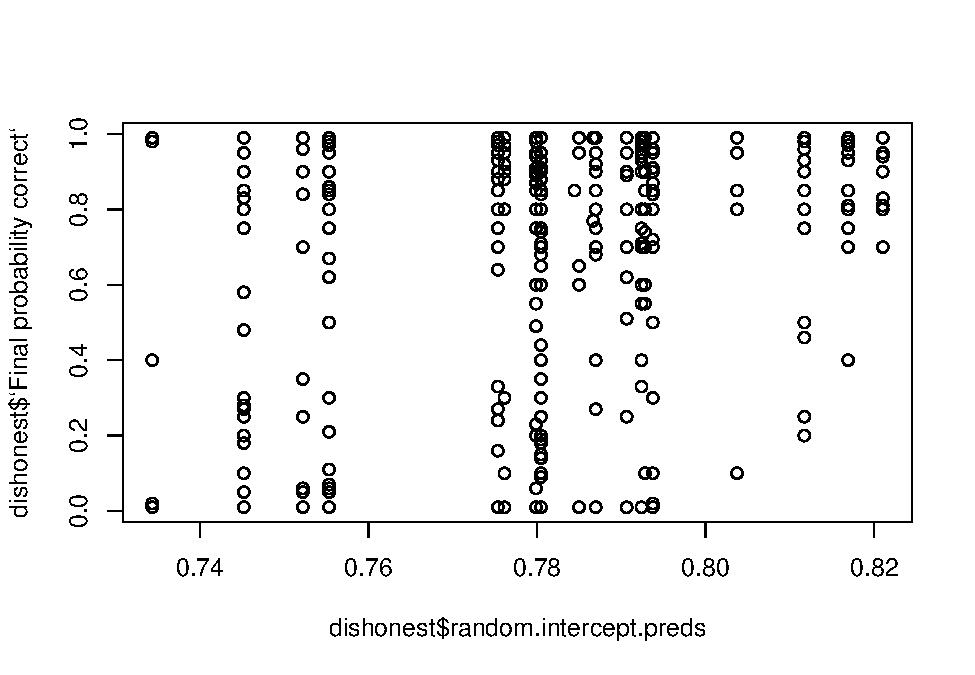
\includegraphics{debate-2309_files/figure-latex/unnamed-chunk-3-9.pdf}

\subsubsection{Debater ``Experience'', ratings - how many
wins?}\label{debater-experience-ratings---how-many-wins}

\subsubsection{AI vs Humans}\label{ai-vs-humans}

\subsubsection{Old vs New}\label{old-vs-new}

\subsubsection{possibly unnessary}\label{possibly-unnessary}

Finally, these are how many we get correct in each setting

\begin{Shaded}
\begin{Highlighting}[]
\NormalTok{judgments\_online }\OtherTok{\textless{}{-}}\NormalTok{ py}\SpecialCharTok{$}\NormalTok{judgments\_online}
\FunctionTok{table}\NormalTok{(judgments\_online}\SpecialCharTok{$}\NormalTok{Final\_Accuracy, judgments\_online}\SpecialCharTok{$}\NormalTok{Final\_Setting)}
\end{Highlighting}
\end{Shaded}

\begin{verbatim}
##        
##         AI Consultancy AI Debate Human Consultancy Human Debate
##   FALSE             18        19                32           25
##   TRUE              75        68                75          130
\end{verbatim}

\begin{Shaded}
\begin{Highlighting}[]
\FunctionTok{table}\NormalTok{(judgments\_online}\SpecialCharTok{$}\NormalTok{Final\_Accuracy, judgments\_online}\SpecialCharTok{$}\NormalTok{Setting)}
\end{Highlighting}
\end{Shaded}

\begin{verbatim}
##        
##         AI Consultancy Dishonest AI Consultancy Honest AI Debate
##   FALSE                        5                    13        19
##   TRUE                        33                    42        68
##        
##         Human Consultancy Dishonest Human Consultancy Honest Human Debate
##   FALSE                          26                        6           25
##   TRUE                           33                       42          130
\end{verbatim}

\begin{Shaded}
\begin{Highlighting}[]
\FunctionTok{ggplot}\NormalTok{(judgments\_online, }\FunctionTok{aes}\NormalTok{(}\AttributeTok{x =}\NormalTok{ Final\_Setting, }\AttributeTok{fill =}\NormalTok{ Final\_Accuracy)) }\SpecialCharTok{+}
  \FunctionTok{geom\_bar}\NormalTok{(}\AttributeTok{position =} \StringTok{"fill"}\NormalTok{) }\SpecialCharTok{+}
  \FunctionTok{scale\_fill\_manual}\NormalTok{(}\AttributeTok{values =} \FunctionTok{c}\NormalTok{(}\StringTok{"TRUE"} \OtherTok{=} \StringTok{"green"}\NormalTok{, }\StringTok{"FALSE"} \OtherTok{=} \StringTok{"red"}\NormalTok{)) }\SpecialCharTok{+}
  \FunctionTok{labs}\NormalTok{(}\AttributeTok{title =} \StringTok{"Judgments by Setting, overall"}\NormalTok{, }\AttributeTok{x =} \StringTok{"Setting"}\NormalTok{, }\AttributeTok{y =} \StringTok{"Proportion"}\NormalTok{, }\AttributeTok{fill =} \StringTok{"Final\_Accuracy"}\NormalTok{) }\SpecialCharTok{+}
  \FunctionTok{theme\_minimal}\NormalTok{() }\SpecialCharTok{+}
  \FunctionTok{theme}\NormalTok{(}\AttributeTok{axis.text.x =} \FunctionTok{element\_text}\NormalTok{())}
\end{Highlighting}
\end{Shaded}

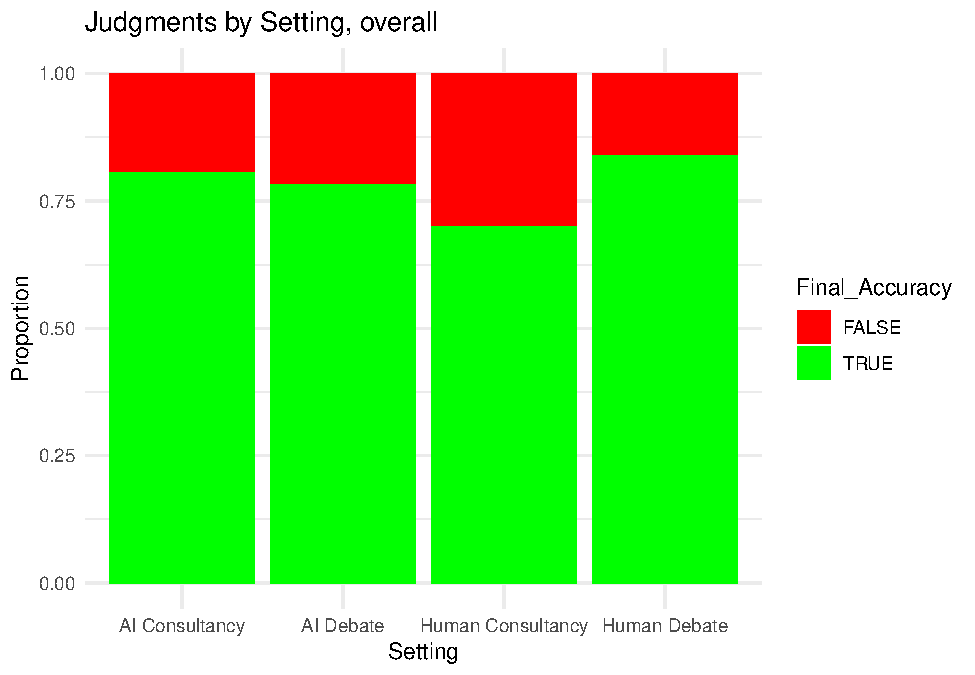
\includegraphics[width=1\linewidth]{debate-2309_files/figure-latex/quick ori acc stats-1}

Sneak peak of accuracy differences between judges, but we won't get to
that again until models

\begin{Shaded}
\begin{Highlighting}[]
\FunctionTok{ggplot}\NormalTok{(judgments\_online, }\FunctionTok{aes}\NormalTok{(}\AttributeTok{x =}\NormalTok{ Final\_Setting, }\AttributeTok{fill =}\NormalTok{ Final\_Accuracy)) }\SpecialCharTok{+}
  \FunctionTok{geom\_bar}\NormalTok{(}\AttributeTok{position =} \StringTok{"fill"}\NormalTok{) }\SpecialCharTok{+}
  \FunctionTok{scale\_fill\_manual}\NormalTok{(}\AttributeTok{values =} \FunctionTok{c}\NormalTok{(}\StringTok{"TRUE"} \OtherTok{=} \StringTok{"green"}\NormalTok{, }\StringTok{"FALSE"} \OtherTok{=} \StringTok{"red"}\NormalTok{)) }\SpecialCharTok{+}
  \FunctionTok{labs}\NormalTok{(}\AttributeTok{title =} \StringTok{"Judgments by Setting, per judge"}\NormalTok{, }\AttributeTok{x =} \StringTok{"Setting"}\NormalTok{, }\AttributeTok{y =} \StringTok{"Proportion"}\NormalTok{, }\AttributeTok{fill =} \StringTok{"Final\_Accuracy"}\NormalTok{) }\SpecialCharTok{+}
  \FunctionTok{theme\_minimal}\NormalTok{() }\SpecialCharTok{+}
  \FunctionTok{theme}\NormalTok{(}\AttributeTok{axis.text.x =} \FunctionTok{element\_text}\NormalTok{(),}\CommentTok{\#angle = 90, hjust = 1),}
        \AttributeTok{axis.text.y =} \FunctionTok{element\_blank}\NormalTok{(),}
        \AttributeTok{strip.text.y.right =} \FunctionTok{element\_text}\NormalTok{(}\AttributeTok{angle =} \DecValTok{0}\NormalTok{)) }\SpecialCharTok{+}
  \FunctionTok{facet\_grid}\NormalTok{(}\AttributeTok{rows =} \StringTok{"Participant"}\NormalTok{)}
\end{Highlighting}
\end{Shaded}

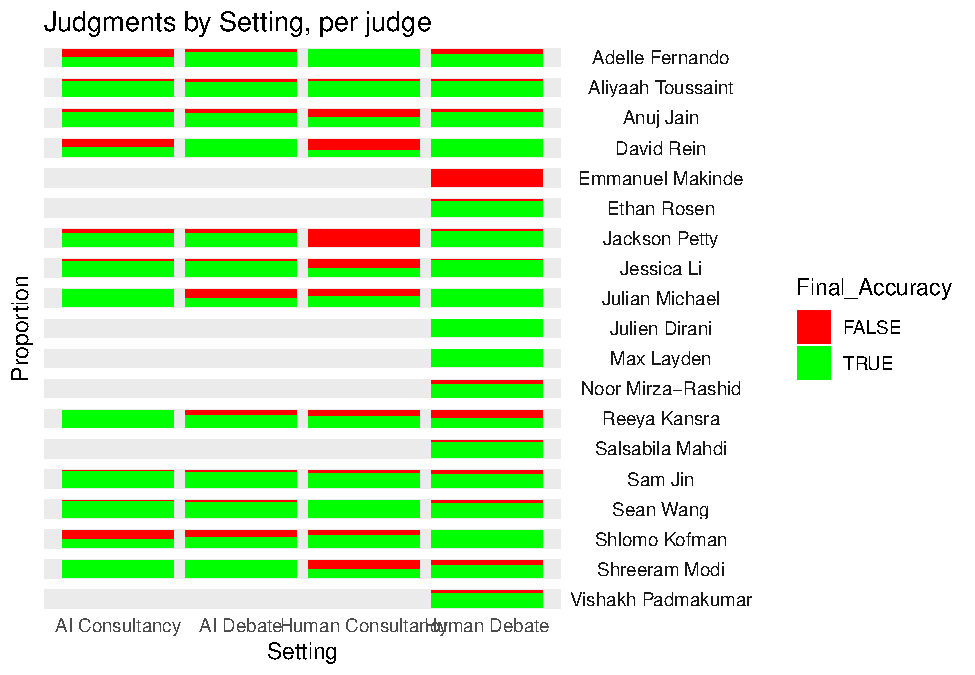
\includegraphics[width=1\linewidth]{debate-2309_files/figure-latex/quick ori stats cont-1}

\end{document}
